\documentclass[oneside]{report}

\usepackage[margin=2cm,nohead]{geometry}
\usepackage[pdftex]{graphicx}
\usepackage{subfig}
\usepackage{float}
\usepackage{verbatim}

\usepackage{hyperref}
\hypersetup{
  colorlinks=true,
  pdfauthor={pmagdon}
  }

\graphicspath{{./graphs/}}


\title{Calibration Report for AWF PAR Sensors}
\author{Paul Magdon}
\date{\today}
\raggedbottom
\setcounter{tocdepth}{1}

\begin{document}

\maketitle

\begin{figure}[H]
  \centering
  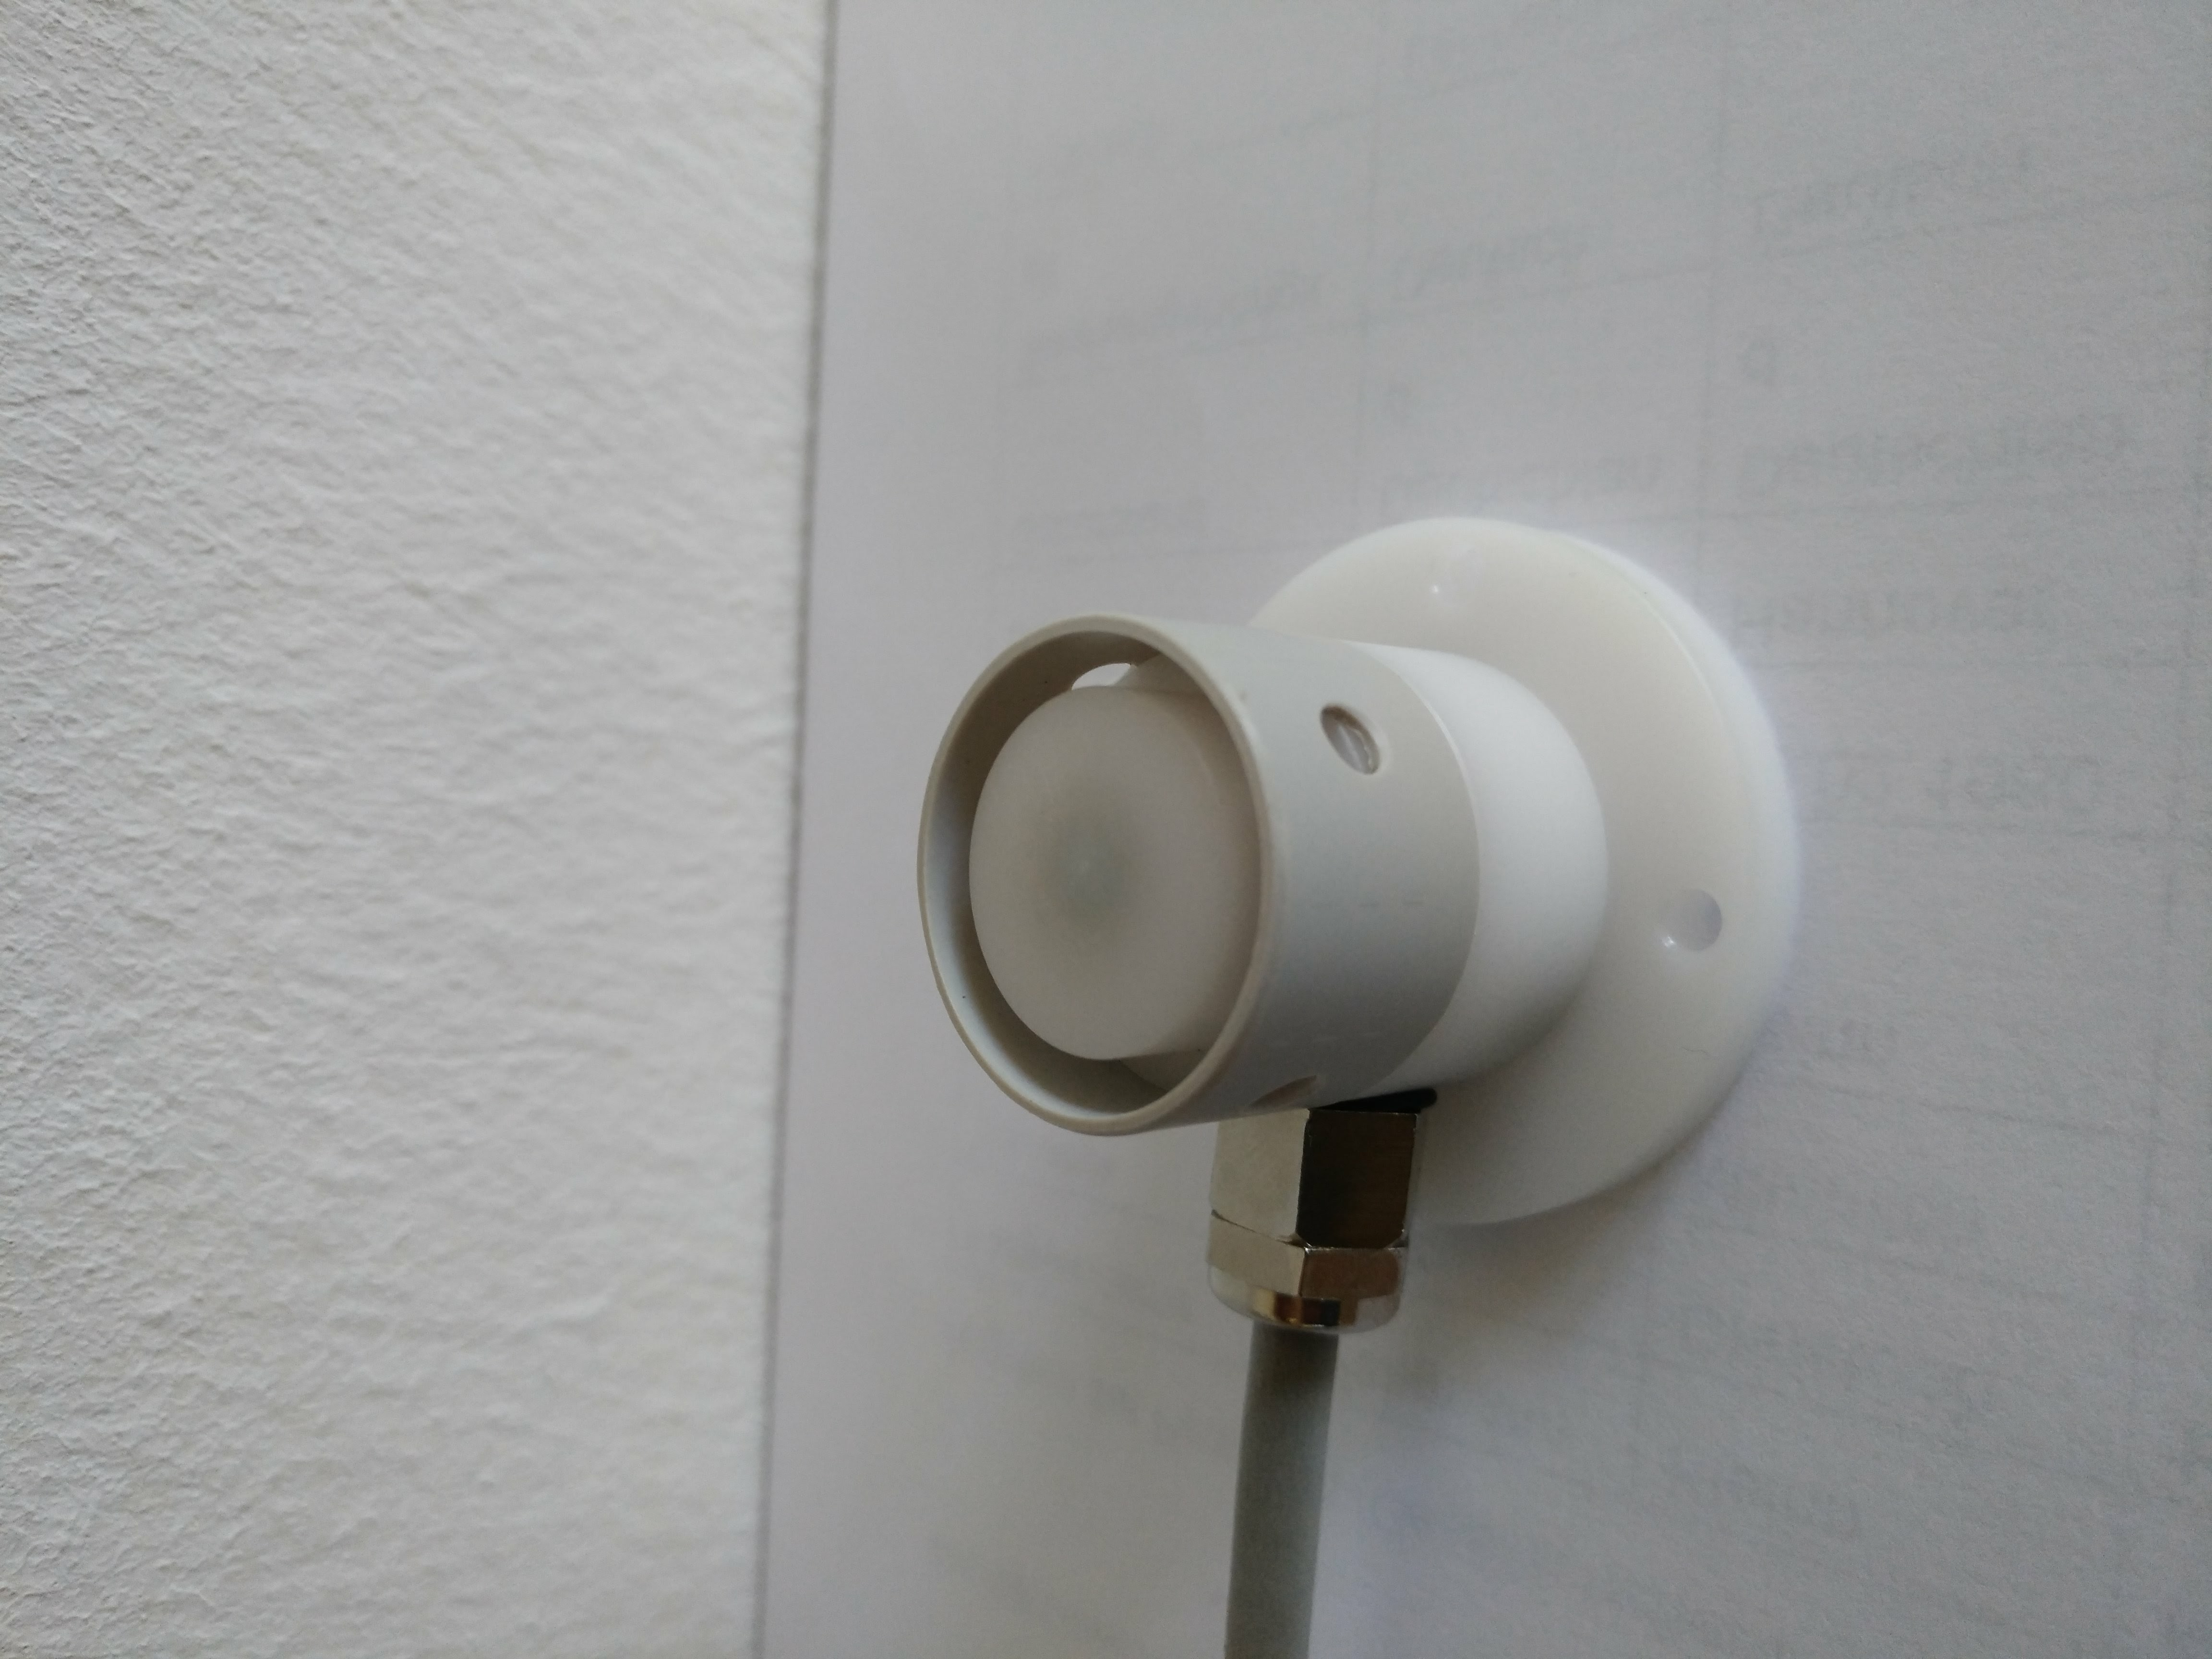
\includegraphics[width=0.5\textwidth,angle=-90]{graphs/sensor.jpg}
	\caption{Custom made PAR Sensor}
\end{figure}

\section*{Background}
For the next phase of the Biodiversity-Exploratories research project all climate stations on the experimental  plots will be equipped with Photosynthetic Active Radiation (PAR) sensors. As the commercially available sensors (e.g. LiCOR LI-190) are quite expensive, we are looking for an alternative. Therefore, we build PAR sensors @ AWF based on a prototype developed and tested by MPI Jena. The calibration of the PAR sensors as presented here had two objectives i) to test the variation between copies of the custom made PAR sensor (PAR-AWF), and ii) to compare the measurement to a calibrated reference.

\section*{Method}
The caluculation of the calibration factors is based on the aggregated 5 Minutes intervalls. We removed the first and last 30 minutes of the time series to avoid disturbances during the set-up of the devices. The calibration coefficients are calculated as the slope of the linear regression model with no intercept. For the analysis and fitting of the linear models all values $\le0.1$ mV were removed as we assume that this is below the sensitivity of the data logger.

\begin{figure}[H]
  \centering
  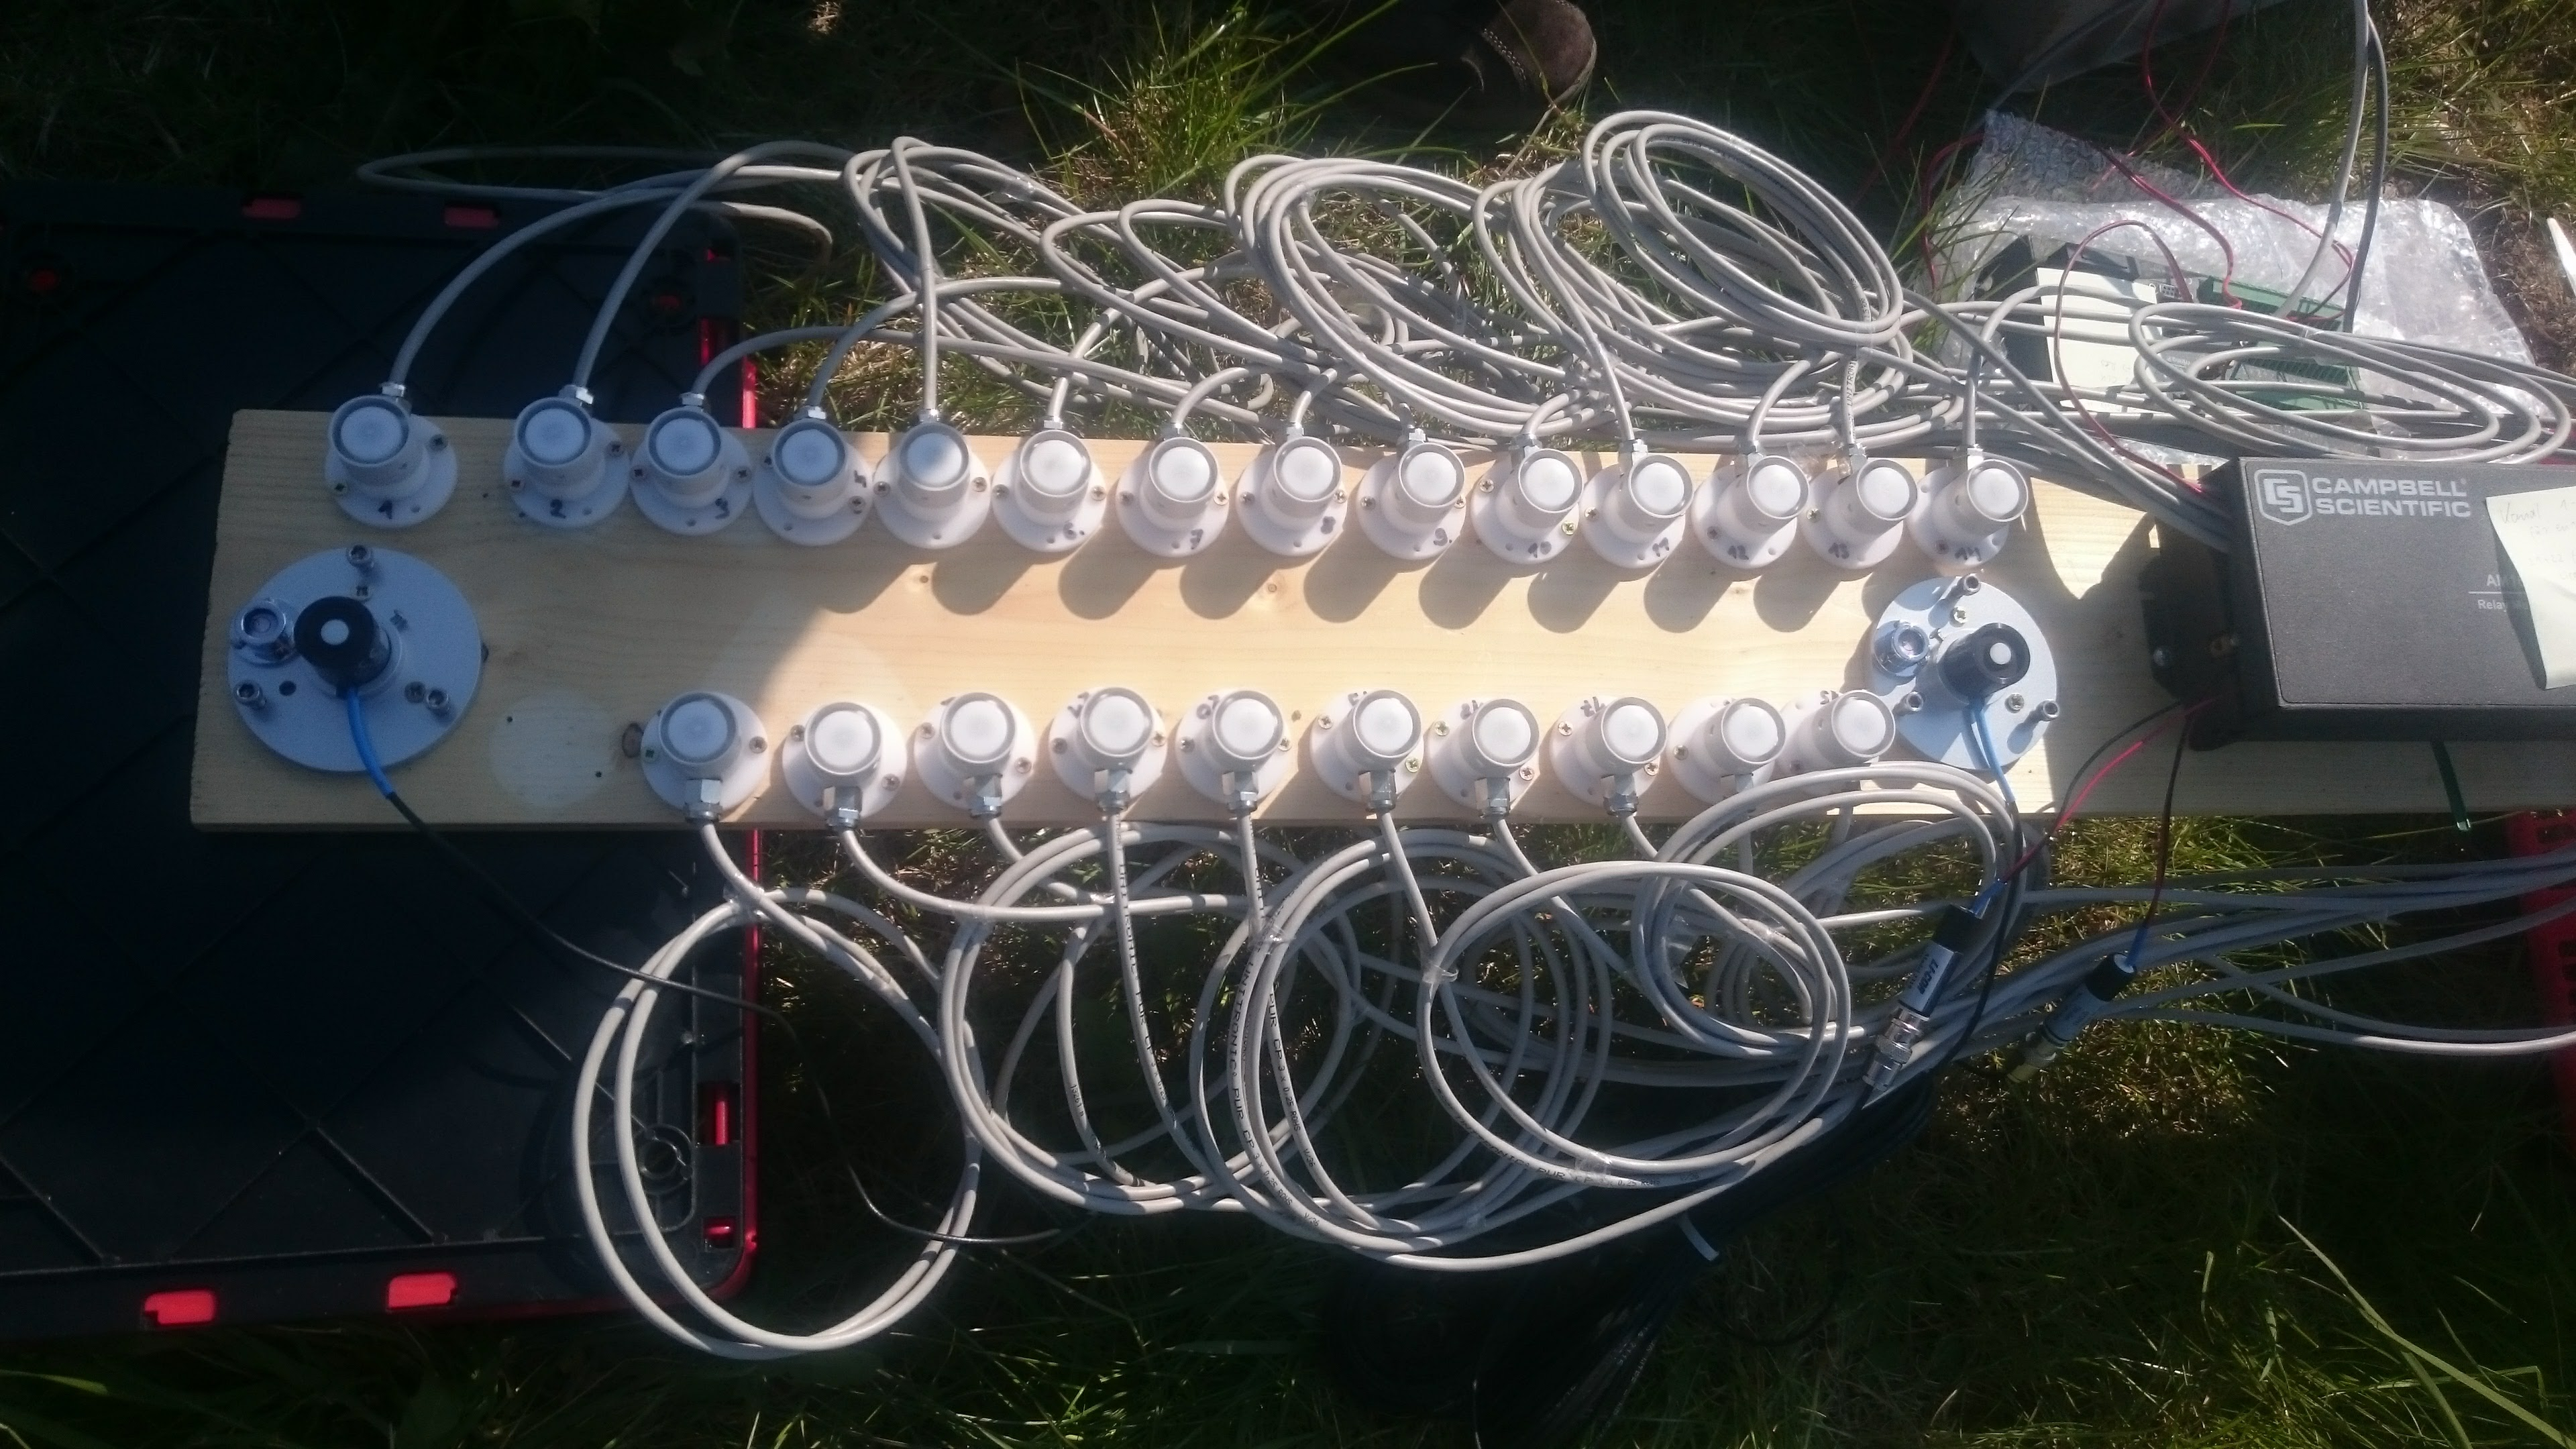
\includegraphics[width=0.6\textwidth]{graphs/Installation.JPG}
	\caption{Calibration setup of Sensors}
\end{figure}




%Import data













% Add two hours as the logger clock was wrong

% Define the reference






% Remove additional columns







% Remove columns where no sensor was connect to the logger from the log file


%Set sensor_ids

















% Set timestamps



%Remove two sensors which were not correctly connected








% Combine all log files

% Set teh refernce by averaging the two Licor sensors


% Create list with all sensor_ids





% Start calculation and report compilation for each sensor
\pagebreak

% Remove values smaller then 0.1

\begin{center}
\large{\textbf{SENSOR:001}}\\
\end{center}

\hrulefill\\
CALIBRATION DATASET:\\
\begin{table}[h!]
  \centering
  \label{tab:table1}
  \begin{tabular}{ll}
    Location: & Aboretum Goettingen\\ 
    
    
    Start:  & Apr 27 09:39:30 2017 \\
    End:   & Apr 28 08:51:30 2017\\ 
    Duration: & 23 h\\
    Measurement frequency: & 0.3hz\\
    Averaging:  &5 min\\
    Number of records: & 169 \\
    References: & LiCOR Q52953, Li-COR Q 52953 \\
  \end{tabular}
\end{table}

\hrulefill\\
CALIBRATION RESULTS:\\
% Define a linear model with the reference as dependent variable and no intersect


\begin{center}
\textbf{\large{Calibration Factor: 50.522}}\\
\end{center}
% latex table generated in R 3.6.3 by xtable 1.8-4 package
% Tue Sep 22 14:16:57 2020
\begin{table}[ht]
\centering
\begin{tabular}{rrrrr}
  \hline
 & Estimate & Std. Error & t value & Pr($>$$|$t$|$) \\ 
  \hline
AWF\_PAR\_001 & 50.5217 & 0.2976 & 169.75 & 0.0000 \\ 
   \hline
\end{tabular}
\end{table}



\hrulefill\\
QUALITY REPORT:\\
Residual standard error: 59.19 PPFD\\
Adjusted R-squared: 0.994



\begin{figure}[H]
  \centering
  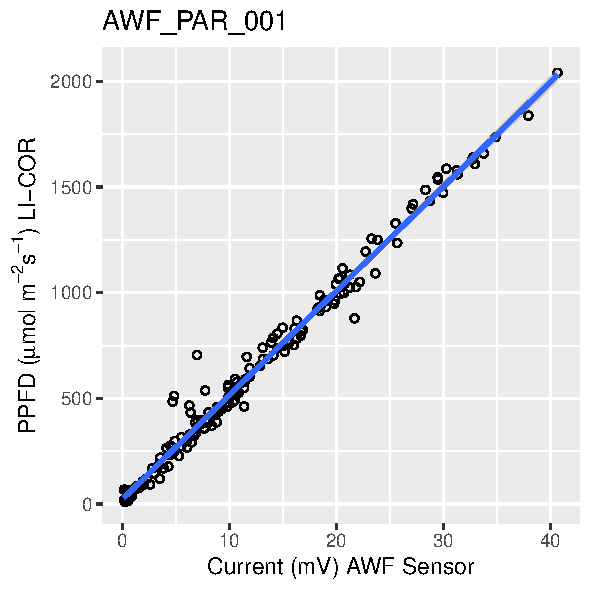
\includegraphics[width=0.4\linewidth]{graphs/AWF_PAR_001_scatter.pdf}
\end{figure}




\begin{figure}[H]
  \centering
  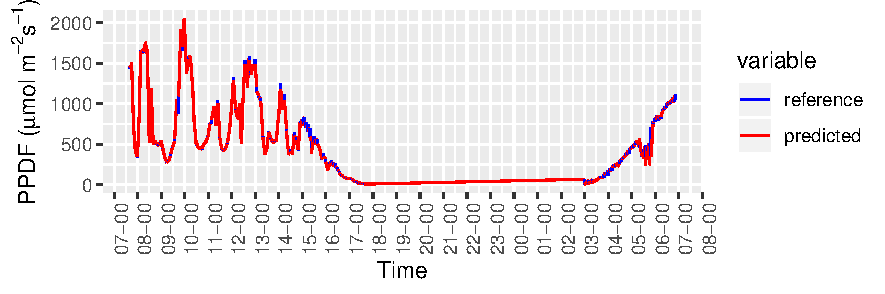
\includegraphics[width=0.7\linewidth]{graphs/AWF_PAR_001_pred.pdf}
\end{figure}

\pagebreak

% Remove values smaller then 0.1

\begin{center}
\large{\textbf{SENSOR:002}}\\
\end{center}

\hrulefill\\
CALIBRATION DATASET:\\
\begin{table}[h!]
  \centering
  \label{tab:table1}
  \begin{tabular}{ll}
    Location: & Aboretum Goettingen\\ 
    
    
    Start:  & Apr 27 09:39:30 2017 \\
    End:   & Apr 28 08:51:30 2017\\ 
    Duration: & 23 h\\
    Measurement frequency: & 0.3hz\\
    Averaging:  &5 min\\
    Number of records: & 169 \\
    References: & LiCOR Q52953, Li-COR Q 52953 \\
  \end{tabular}
\end{table}

\hrulefill\\
CALIBRATION RESULTS:\\
% Define a linear model with the reference as dependent variable and no intersect


\begin{center}
\textbf{\large{Calibration Factor: 51.15}}\\
\end{center}
% latex table generated in R 3.6.3 by xtable 1.8-4 package
% Tue Sep 22 14:16:58 2020
\begin{table}[ht]
\centering
\begin{tabular}{rrrrr}
  \hline
 & Estimate & Std. Error & t value & Pr($>$$|$t$|$) \\ 
  \hline
AWF\_PAR\_002 & 51.1499 & 0.2689 & 190.22 & 0.0000 \\ 
   \hline
\end{tabular}
\end{table}



\hrulefill\\
QUALITY REPORT:\\
Residual standard error: 52.85 PPFD\\
Adjusted R-squared: 0.995



\begin{figure}[H]
  \centering
  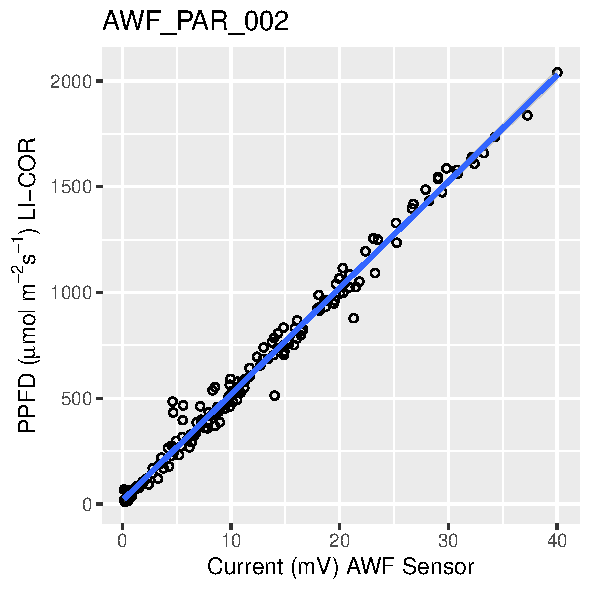
\includegraphics[width=0.4\linewidth]{graphs/AWF_PAR_002_scatter.pdf}
\end{figure}




\begin{figure}[H]
  \centering
  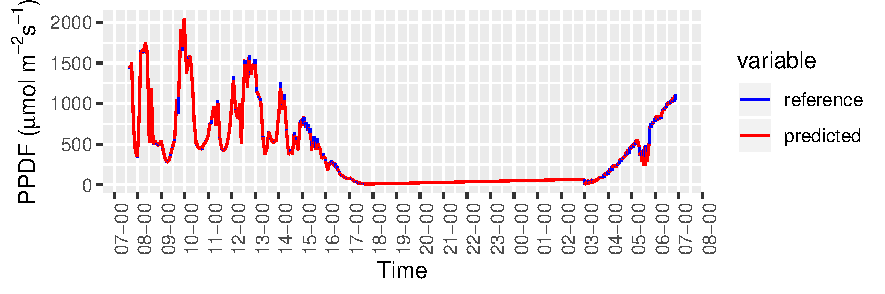
\includegraphics[width=0.7\linewidth]{graphs/AWF_PAR_002_pred.pdf}
\end{figure}

\pagebreak

% Remove values smaller then 0.1

\begin{center}
\large{\textbf{SENSOR:003}}\\
\end{center}

\hrulefill\\
CALIBRATION DATASET:\\
\begin{table}[h!]
  \centering
  \label{tab:table1}
  \begin{tabular}{ll}
    Location: & Aboretum Goettingen\\ 
    
    
    Start:  & Apr 27 09:39:30 2017 \\
    End:   & Apr 28 08:51:30 2017\\ 
    Duration: & 23 h\\
    Measurement frequency: & 0.3hz\\
    Averaging:  &5 min\\
    Number of records: & 170 \\
    References: & LiCOR Q52953, Li-COR Q 52953 \\
  \end{tabular}
\end{table}

\hrulefill\\
CALIBRATION RESULTS:\\
% Define a linear model with the reference as dependent variable and no intersect


\begin{center}
\textbf{\large{Calibration Factor: 49.622}}\\
\end{center}
% latex table generated in R 3.6.3 by xtable 1.8-4 package
% Tue Sep 22 14:16:59 2020
\begin{table}[ht]
\centering
\begin{tabular}{rrrrr}
  \hline
 & Estimate & Std. Error & t value & Pr($>$$|$t$|$) \\ 
  \hline
AWF\_PAR\_003 & 49.6217 & 0.2536 & 195.70 & 0.0000 \\ 
   \hline
\end{tabular}
\end{table}



\hrulefill\\
QUALITY REPORT:\\
Residual standard error: 51.38 PPFD\\
Adjusted R-squared: 0.996



\begin{figure}[H]
  \centering
  \includegraphics[width=0.4\linewidth]{graphs/AWF_PAR_003_scatter.pdf}
\end{figure}




\begin{figure}[H]
  \centering
  \includegraphics[width=0.7\linewidth]{graphs/AWF_PAR_003_pred.pdf}
\end{figure}

\pagebreak

% Remove values smaller then 0.1

\begin{center}
\large{\textbf{SENSOR:004}}\\
\end{center}

\hrulefill\\
CALIBRATION DATASET:\\
\begin{table}[h!]
  \centering
  \label{tab:table1}
  \begin{tabular}{ll}
    Location: & Aboretum Goettingen\\ 
    
    
    Start:  & Apr 27 09:39:30 2017 \\
    End:   & Apr 28 08:51:30 2017\\ 
    Duration: & 23 h\\
    Measurement frequency: & 0.3hz\\
    Averaging:  &5 min\\
    Number of records: & 170 \\
    References: & LiCOR Q52953, Li-COR Q 52953 \\
  \end{tabular}
\end{table}

\hrulefill\\
CALIBRATION RESULTS:\\
% Define a linear model with the reference as dependent variable and no intersect


\begin{center}
\textbf{\large{Calibration Factor: 47.806}}\\
\end{center}
% latex table generated in R 3.6.3 by xtable 1.8-4 package
% Tue Sep 22 14:16:59 2020
\begin{table}[ht]
\centering
\begin{tabular}{rrrrr}
  \hline
 & Estimate & Std. Error & t value & Pr($>$$|$t$|$) \\ 
  \hline
AWF\_PAR\_004 & 47.8061 & 0.3000 & 159.35 & 0.0000 \\ 
   \hline
\end{tabular}
\end{table}



\hrulefill\\
QUALITY REPORT:\\
Residual standard error: 63.02 PPFD\\
Adjusted R-squared: 0.993



\begin{figure}[H]
  \centering
  \includegraphics[width=0.4\linewidth]{graphs/AWF_PAR_004_scatter.pdf}
\end{figure}




\begin{figure}[H]
  \centering
  \includegraphics[width=0.7\linewidth]{graphs/AWF_PAR_004_pred.pdf}
\end{figure}

\pagebreak

% Remove values smaller then 0.1

\begin{center}
\large{\textbf{SENSOR:005}}\\
\end{center}

\hrulefill\\
CALIBRATION DATASET:\\
\begin{table}[h!]
  \centering
  \label{tab:table1}
  \begin{tabular}{ll}
    Location: & Aboretum Goettingen\\ 
    
    
    Start:  & Apr 27 09:39:30 2017 \\
    End:   & Apr 28 08:51:30 2017\\ 
    Duration: & 23 h\\
    Measurement frequency: & 0.3hz\\
    Averaging:  &5 min\\
    Number of records: & 169 \\
    References: & LiCOR Q52953, Li-COR Q 52953 \\
  \end{tabular}
\end{table}

\hrulefill\\
CALIBRATION RESULTS:\\
% Define a linear model with the reference as dependent variable and no intersect


\begin{center}
\textbf{\large{Calibration Factor: 50.249}}\\
\end{center}
% latex table generated in R 3.6.3 by xtable 1.8-4 package
% Tue Sep 22 14:17:00 2020
\begin{table}[ht]
\centering
\begin{tabular}{rrrrr}
  \hline
 & Estimate & Std. Error & t value & Pr($>$$|$t$|$) \\ 
  \hline
AWF\_PAR\_005 & 50.2494 & 0.3686 & 136.31 & 0.0000 \\ 
   \hline
\end{tabular}
\end{table}



\hrulefill\\
QUALITY REPORT:\\
Residual standard error: 73.59 PPFD\\
Adjusted R-squared: 0.991



\begin{figure}[H]
  \centering
  \includegraphics[width=0.4\linewidth]{graphs/AWF_PAR_005_scatter.pdf}
\end{figure}




\begin{figure}[H]
  \centering
  \includegraphics[width=0.7\linewidth]{graphs/AWF_PAR_005_pred.pdf}
\end{figure}

\pagebreak

% Remove values smaller then 0.1

\begin{center}
\large{\textbf{SENSOR:006}}\\
\end{center}

\hrulefill\\
CALIBRATION DATASET:\\
\begin{table}[h!]
  \centering
  \label{tab:table1}
  \begin{tabular}{ll}
    Location: & Aboretum Goettingen\\ 
    
    
    Start:  & Apr 27 09:39:30 2017 \\
    End:   & Apr 28 08:51:30 2017\\ 
    Duration: & 23 h\\
    Measurement frequency: & 0.3hz\\
    Averaging:  &5 min\\
    Number of records: & 169 \\
    References: & LiCOR Q52953, Li-COR Q 52953 \\
  \end{tabular}
\end{table}

\hrulefill\\
CALIBRATION RESULTS:\\
% Define a linear model with the reference as dependent variable and no intersect


\begin{center}
\textbf{\large{Calibration Factor: 52.535}}\\
\end{center}
% latex table generated in R 3.6.3 by xtable 1.8-4 package
% Tue Sep 22 14:17:00 2020
\begin{table}[ht]
\centering
\begin{tabular}{rrrrr}
  \hline
 & Estimate & Std. Error & t value & Pr($>$$|$t$|$) \\ 
  \hline
AWF\_PAR\_006 & 52.5353 & 0.3338 & 157.39 & 0.0000 \\ 
   \hline
\end{tabular}
\end{table}



\hrulefill\\
QUALITY REPORT:\\
Residual standard error: 63.81 PPFD\\
Adjusted R-squared: 0.993



\begin{figure}[H]
  \centering
  \includegraphics[width=0.4\linewidth]{graphs/AWF_PAR_006_scatter.pdf}
\end{figure}




\begin{figure}[H]
  \centering
  \includegraphics[width=0.7\linewidth]{graphs/AWF_PAR_006_pred.pdf}
\end{figure}

\pagebreak

% Remove values smaller then 0.1

\begin{center}
\large{\textbf{SENSOR:007}}\\
\end{center}

\hrulefill\\
CALIBRATION DATASET:\\
\begin{table}[h!]
  \centering
  \label{tab:table1}
  \begin{tabular}{ll}
    Location: & Aboretum Goettingen\\ 
    
    
    Start:  & Apr 27 09:39:30 2017 \\
    End:   & Apr 28 08:51:30 2017\\ 
    Duration: & 23 h\\
    Measurement frequency: & 0.3hz\\
    Averaging:  &5 min\\
    Number of records: & 170 \\
    References: & LiCOR Q52953, Li-COR Q 52953 \\
  \end{tabular}
\end{table}

\hrulefill\\
CALIBRATION RESULTS:\\
% Define a linear model with the reference as dependent variable and no intersect


\begin{center}
\textbf{\large{Calibration Factor: 47.33}}\\
\end{center}
% latex table generated in R 3.6.3 by xtable 1.8-4 package
% Tue Sep 22 14:17:01 2020
\begin{table}[ht]
\centering
\begin{tabular}{rrrrr}
  \hline
 & Estimate & Std. Error & t value & Pr($>$$|$t$|$) \\ 
  \hline
AWF\_PAR\_007 & 47.3304 & 0.3001 & 157.74 & 0.0000 \\ 
   \hline
\end{tabular}
\end{table}



\hrulefill\\
QUALITY REPORT:\\
Residual standard error: 63.67 PPFD\\
Adjusted R-squared: 0.993



\begin{figure}[H]
  \centering
  \includegraphics[width=0.4\linewidth]{graphs/AWF_PAR_007_scatter.pdf}
\end{figure}




\begin{figure}[H]
  \centering
  \includegraphics[width=0.7\linewidth]{graphs/AWF_PAR_007_pred.pdf}
\end{figure}

\pagebreak

% Remove values smaller then 0.1

\begin{center}
\large{\textbf{SENSOR:008}}\\
\end{center}

\hrulefill\\
CALIBRATION DATASET:\\
\begin{table}[h!]
  \centering
  \label{tab:table1}
  \begin{tabular}{ll}
    Location: & Aboretum Goettingen\\ 
    
    
    Start:  & Apr 27 09:39:30 2017 \\
    End:   & Apr 28 08:51:30 2017\\ 
    Duration: & 23 h\\
    Measurement frequency: & 0.3hz\\
    Averaging:  &5 min\\
    Number of records: & 170 \\
    References: & LiCOR Q52953, Li-COR Q 52953 \\
  \end{tabular}
\end{table}

\hrulefill\\
CALIBRATION RESULTS:\\
% Define a linear model with the reference as dependent variable and no intersect


\begin{center}
\textbf{\large{Calibration Factor: 47.27}}\\
\end{center}
% latex table generated in R 3.6.3 by xtable 1.8-4 package
% Tue Sep 22 14:17:02 2020
\begin{table}[ht]
\centering
\begin{tabular}{rrrrr}
  \hline
 & Estimate & Std. Error & t value & Pr($>$$|$t$|$) \\ 
  \hline
AWF\_PAR\_008 & 47.2704 & 0.2723 & 173.57 & 0.0000 \\ 
   \hline
\end{tabular}
\end{table}



\hrulefill\\
QUALITY REPORT:\\
Residual standard error: 57.89 PPFD\\
Adjusted R-squared: 0.994



\begin{figure}[H]
  \centering
  \includegraphics[width=0.4\linewidth]{graphs/AWF_PAR_008_scatter.pdf}
\end{figure}




\begin{figure}[H]
  \centering
  \includegraphics[width=0.7\linewidth]{graphs/AWF_PAR_008_pred.pdf}
\end{figure}

\pagebreak

% Remove values smaller then 0.1

\begin{center}
\large{\textbf{SENSOR:009}}\\
\end{center}

\hrulefill\\
CALIBRATION DATASET:\\
\begin{table}[h!]
  \centering
  \label{tab:table1}
  \begin{tabular}{ll}
    Location: & Aboretum Goettingen\\ 
    
    
    Start:  & Apr 27 09:39:30 2017 \\
    End:   & Apr 28 08:51:30 2017\\ 
    Duration: & 23 h\\
    Measurement frequency: & 0.3hz\\
    Averaging:  &5 min\\
    Number of records: & 170 \\
    References: & LiCOR Q52953, Li-COR Q 52953 \\
  \end{tabular}
\end{table}

\hrulefill\\
CALIBRATION RESULTS:\\
% Define a linear model with the reference as dependent variable and no intersect


\begin{center}
\textbf{\large{Calibration Factor: 47.199}}\\
\end{center}
% latex table generated in R 3.6.3 by xtable 1.8-4 package
% Tue Sep 22 14:17:02 2020
\begin{table}[ht]
\centering
\begin{tabular}{rrrrr}
  \hline
 & Estimate & Std. Error & t value & Pr($>$$|$t$|$) \\ 
  \hline
AWF\_PAR\_009 & 47.1995 & 0.2552 & 184.93 & 0.0000 \\ 
   \hline
\end{tabular}
\end{table}



\hrulefill\\
QUALITY REPORT:\\
Residual standard error: 54.35 PPFD\\
Adjusted R-squared: 0.995



\begin{figure}[H]
  \centering
  \includegraphics[width=0.4\linewidth]{graphs/AWF_PAR_009_scatter.pdf}
\end{figure}




\begin{figure}[H]
  \centering
  \includegraphics[width=0.7\linewidth]{graphs/AWF_PAR_009_pred.pdf}
\end{figure}

\pagebreak

% Remove values smaller then 0.1

\begin{center}
\large{\textbf{SENSOR:010}}\\
\end{center}

\hrulefill\\
CALIBRATION DATASET:\\
\begin{table}[h!]
  \centering
  \label{tab:table1}
  \begin{tabular}{ll}
    Location: & Aboretum Goettingen\\ 
    
    
    Start:  & Apr 27 09:39:30 2017 \\
    End:   & Apr 28 08:51:30 2017\\ 
    Duration: & 23 h\\
    Measurement frequency: & 0.3hz\\
    Averaging:  &5 min\\
    Number of records: & 169 \\
    References: & LiCOR Q52953, Li-COR Q 52953 \\
  \end{tabular}
\end{table}

\hrulefill\\
CALIBRATION RESULTS:\\
% Define a linear model with the reference as dependent variable and no intersect


\begin{center}
\textbf{\large{Calibration Factor: 51.08}}\\
\end{center}
% latex table generated in R 3.6.3 by xtable 1.8-4 package
% Tue Sep 22 14:17:03 2020
\begin{table}[ht]
\centering
\begin{tabular}{rrrrr}
  \hline
 & Estimate & Std. Error & t value & Pr($>$$|$t$|$) \\ 
  \hline
AWF\_PAR\_010 & 51.0795 & 0.2479 & 206.02 & 0.0000 \\ 
   \hline
\end{tabular}
\end{table}



\hrulefill\\
QUALITY REPORT:\\
Residual standard error: 48.81 PPFD\\
Adjusted R-squared: 0.996



\begin{figure}[H]
  \centering
  \includegraphics[width=0.4\linewidth]{graphs/AWF_PAR_010_scatter.pdf}
\end{figure}




\begin{figure}[H]
  \centering
  \includegraphics[width=0.7\linewidth]{graphs/AWF_PAR_010_pred.pdf}
\end{figure}

\pagebreak

% Remove values smaller then 0.1

\begin{center}
\large{\textbf{SENSOR:011}}\\
\end{center}

\hrulefill\\
CALIBRATION DATASET:\\
\begin{table}[h!]
  \centering
  \label{tab:table1}
  \begin{tabular}{ll}
    Location: & Aboretum Goettingen\\ 
    
    
    Start:  & Apr 27 09:39:30 2017 \\
    End:   & Apr 28 08:51:30 2017\\ 
    Duration: & 23 h\\
    Measurement frequency: & 0.3hz\\
    Averaging:  &5 min\\
    Number of records: & 170 \\
    References: & LiCOR Q52953, Li-COR Q 52953 \\
  \end{tabular}
\end{table}

\hrulefill\\
CALIBRATION RESULTS:\\
% Define a linear model with the reference as dependent variable and no intersect


\begin{center}
\textbf{\large{Calibration Factor: 46.423}}\\
\end{center}
% latex table generated in R 3.6.3 by xtable 1.8-4 package
% Tue Sep 22 14:17:03 2020
\begin{table}[ht]
\centering
\begin{tabular}{rrrrr}
  \hline
 & Estimate & Std. Error & t value & Pr($>$$|$t$|$) \\ 
  \hline
AWF\_PAR\_011 & 46.4228 & 0.2082 & 223.00 & 0.0000 \\ 
   \hline
\end{tabular}
\end{table}



\hrulefill\\
QUALITY REPORT:\\
Residual standard error: 45.11 PPFD\\
Adjusted R-squared: 0.997



\begin{figure}[H]
  \centering
  \includegraphics[width=0.4\linewidth]{graphs/AWF_PAR_011_scatter.pdf}
\end{figure}




\begin{figure}[H]
  \centering
  \includegraphics[width=0.7\linewidth]{graphs/AWF_PAR_011_pred.pdf}
\end{figure}

\pagebreak

% Remove values smaller then 0.1

\begin{center}
\large{\textbf{SENSOR:012}}\\
\end{center}

\hrulefill\\
CALIBRATION DATASET:\\
\begin{table}[h!]
  \centering
  \label{tab:table1}
  \begin{tabular}{ll}
    Location: & Aboretum Goettingen\\ 
    
    
    Start:  & Apr 27 09:39:30 2017 \\
    End:   & Apr 28 08:51:30 2017\\ 
    Duration: & 23 h\\
    Measurement frequency: & 0.3hz\\
    Averaging:  &5 min\\
    Number of records: & 170 \\
    References: & LiCOR Q52953, Li-COR Q 52953 \\
  \end{tabular}
\end{table}

\hrulefill\\
CALIBRATION RESULTS:\\
% Define a linear model with the reference as dependent variable and no intersect


\begin{center}
\textbf{\large{Calibration Factor: 47.36}}\\
\end{center}
% latex table generated in R 3.6.3 by xtable 1.8-4 package
% Tue Sep 22 14:17:03 2020
\begin{table}[ht]
\centering
\begin{tabular}{rrrrr}
  \hline
 & Estimate & Std. Error & t value & Pr($>$$|$t$|$) \\ 
  \hline
AWF\_PAR\_012 & 47.3596 & 0.2107 & 224.82 & 0.0000 \\ 
   \hline
\end{tabular}
\end{table}



\hrulefill\\
QUALITY REPORT:\\
Residual standard error: 44.74 PPFD\\
Adjusted R-squared: 0.997



\begin{figure}[H]
  \centering
  \includegraphics[width=0.4\linewidth]{graphs/AWF_PAR_012_scatter.pdf}
\end{figure}




\begin{figure}[H]
  \centering
  \includegraphics[width=0.7\linewidth]{graphs/AWF_PAR_012_pred.pdf}
\end{figure}

\pagebreak

% Remove values smaller then 0.1

\begin{center}
\large{\textbf{SENSOR:013}}\\
\end{center}

\hrulefill\\
CALIBRATION DATASET:\\
\begin{table}[h!]
  \centering
  \label{tab:table1}
  \begin{tabular}{ll}
    Location: & Aboretum Goettingen\\ 
    
    
    Start:  & Apr 27 09:39:30 2017 \\
    End:   & Apr 28 08:51:30 2017\\ 
    Duration: & 23 h\\
    Measurement frequency: & 0.3hz\\
    Averaging:  &5 min\\
    Number of records: & 170 \\
    References: & LiCOR Q52953, Li-COR Q 52953 \\
  \end{tabular}
\end{table}

\hrulefill\\
CALIBRATION RESULTS:\\
% Define a linear model with the reference as dependent variable and no intersect


\begin{center}
\textbf{\large{Calibration Factor: 48.642}}\\
\end{center}
% latex table generated in R 3.6.3 by xtable 1.8-4 package
% Tue Sep 22 14:17:04 2020
\begin{table}[ht]
\centering
\begin{tabular}{rrrrr}
  \hline
 & Estimate & Std. Error & t value & Pr($>$$|$t$|$) \\ 
  \hline
AWF\_PAR\_013 & 48.6423 & 0.1877 & 259.14 & 0.0000 \\ 
   \hline
\end{tabular}
\end{table}



\hrulefill\\
QUALITY REPORT:\\
Residual standard error: 38.84 PPFD\\
Adjusted R-squared: 0.997



\begin{figure}[H]
  \centering
  \includegraphics[width=0.4\linewidth]{graphs/AWF_PAR_013_scatter.pdf}
\end{figure}




\begin{figure}[H]
  \centering
  \includegraphics[width=0.7\linewidth]{graphs/AWF_PAR_013_pred.pdf}
\end{figure}

\pagebreak

% Remove values smaller then 0.1

\begin{center}
\large{\textbf{SENSOR:014}}\\
\end{center}

\hrulefill\\
CALIBRATION DATASET:\\
\begin{table}[h!]
  \centering
  \label{tab:table1}
  \begin{tabular}{ll}
    Location: & Aboretum Goettingen\\ 
    
    
    Start:  & Apr 27 09:39:30 2017 \\
    End:   & Apr 28 08:51:30 2017\\ 
    Duration: & 23 h\\
    Measurement frequency: & 0.3hz\\
    Averaging:  &5 min\\
    Number of records: & 170 \\
    References: & LiCOR Q52953, Li-COR Q 52953 \\
  \end{tabular}
\end{table}

\hrulefill\\
CALIBRATION RESULTS:\\
% Define a linear model with the reference as dependent variable and no intersect


\begin{center}
\textbf{\large{Calibration Factor: 49.232}}\\
\end{center}
% latex table generated in R 3.6.3 by xtable 1.8-4 package
% Tue Sep 22 14:17:04 2020
\begin{table}[ht]
\centering
\begin{tabular}{rrrrr}
  \hline
 & Estimate & Std. Error & t value & Pr($>$$|$t$|$) \\ 
  \hline
AWF\_PAR\_014 & 49.2324 & 0.1793 & 274.65 & 0.0000 \\ 
   \hline
\end{tabular}
\end{table}



\hrulefill\\
QUALITY REPORT:\\
Residual standard error: 36.65 PPFD\\
Adjusted R-squared: 0.998



\begin{figure}[H]
  \centering
  \includegraphics[width=0.4\linewidth]{graphs/AWF_PAR_014_scatter.pdf}
\end{figure}




\begin{figure}[H]
  \centering
  \includegraphics[width=0.7\linewidth]{graphs/AWF_PAR_014_pred.pdf}
\end{figure}

\pagebreak

% Remove values smaller then 0.1

\begin{center}
\large{\textbf{SENSOR:015}}\\
\end{center}

\hrulefill\\
CALIBRATION DATASET:\\
\begin{table}[h!]
  \centering
  \label{tab:table1}
  \begin{tabular}{ll}
    Location: & Aboretum Goettingen\\ 
    
    
    Start:  & Apr 27 09:39:30 2017 \\
    End:   & Apr 28 08:51:30 2017\\ 
    Duration: & 23 h\\
    Measurement frequency: & 0.3hz\\
    Averaging:  &5 min\\
    Number of records: & 170 \\
    References: & LiCOR Q52953, Li-COR Q 52953 \\
  \end{tabular}
\end{table}

\hrulefill\\
CALIBRATION RESULTS:\\
% Define a linear model with the reference as dependent variable and no intersect


\begin{center}
\textbf{\large{Calibration Factor: 46.295}}\\
\end{center}
% latex table generated in R 3.6.3 by xtable 1.8-4 package
% Tue Sep 22 14:17:05 2020
\begin{table}[ht]
\centering
\begin{tabular}{rrrrr}
  \hline
 & Estimate & Std. Error & t value & Pr($>$$|$t$|$) \\ 
  \hline
AWF\_PAR\_015 & 46.2952 & 0.1914 & 241.88 & 0.0000 \\ 
   \hline
\end{tabular}
\end{table}



\hrulefill\\
QUALITY REPORT:\\
Residual standard error: 41.6 PPFD\\
Adjusted R-squared: 0.997



\begin{figure}[H]
  \centering
  \includegraphics[width=0.4\linewidth]{graphs/AWF_PAR_015_scatter.pdf}
\end{figure}




\begin{figure}[H]
  \centering
  \includegraphics[width=0.7\linewidth]{graphs/AWF_PAR_015_pred.pdf}
\end{figure}

\pagebreak

% Remove values smaller then 0.1

\begin{center}
\large{\textbf{SENSOR:016}}\\
\end{center}

\hrulefill\\
CALIBRATION DATASET:\\
\begin{table}[h!]
  \centering
  \label{tab:table1}
  \begin{tabular}{ll}
    Location: & Aboretum Goettingen\\ 
    
    
    Start:  & Apr 27 09:39:30 2017 \\
    End:   & Apr 28 08:51:30 2017\\ 
    Duration: & 23 h\\
    Measurement frequency: & 0.3hz\\
    Averaging:  &5 min\\
    Number of records: & 169 \\
    References: & LiCOR Q52953, Li-COR Q 52953 \\
  \end{tabular}
\end{table}

\hrulefill\\
CALIBRATION RESULTS:\\
% Define a linear model with the reference as dependent variable and no intersect


\begin{center}
\textbf{\large{Calibration Factor: 48.89}}\\
\end{center}
% latex table generated in R 3.6.3 by xtable 1.8-4 package
% Tue Sep 22 14:17:06 2020
\begin{table}[ht]
\centering
\begin{tabular}{rrrrr}
  \hline
 & Estimate & Std. Error & t value & Pr($>$$|$t$|$) \\ 
  \hline
AWF\_PAR\_016 & 48.8902 & 0.1991 & 245.53 & 0.0000 \\ 
   \hline
\end{tabular}
\end{table}



\hrulefill\\
QUALITY REPORT:\\
Residual standard error: 40.98 PPFD\\
Adjusted R-squared: 0.997



\begin{figure}[H]
  \centering
  \includegraphics[width=0.4\linewidth]{graphs/AWF_PAR_016_scatter.pdf}
\end{figure}




\begin{figure}[H]
  \centering
  \includegraphics[width=0.7\linewidth]{graphs/AWF_PAR_016_pred.pdf}
\end{figure}

\pagebreak

% Remove values smaller then 0.1

\begin{center}
\large{\textbf{SENSOR:017}}\\
\end{center}

\hrulefill\\
CALIBRATION DATASET:\\
\begin{table}[h!]
  \centering
  \label{tab:table1}
  \begin{tabular}{ll}
    Location: & Aboretum Goettingen\\ 
    
    
    Start:  & Apr 27 09:39:30 2017 \\
    End:   & Apr 28 08:51:30 2017\\ 
    Duration: & 23 h\\
    Measurement frequency: & 0.3hz\\
    Averaging:  &5 min\\
    Number of records: & 170 \\
    References: & LiCOR Q52953, Li-COR Q 52953 \\
  \end{tabular}
\end{table}

\hrulefill\\
CALIBRATION RESULTS:\\
% Define a linear model with the reference as dependent variable and no intersect


\begin{center}
\textbf{\large{Calibration Factor: 47.091}}\\
\end{center}
% latex table generated in R 3.6.3 by xtable 1.8-4 package
% Tue Sep 22 14:17:06 2020
\begin{table}[ht]
\centering
\begin{tabular}{rrrrr}
  \hline
 & Estimate & Std. Error & t value & Pr($>$$|$t$|$) \\ 
  \hline
AWF\_PAR\_017 & 47.0915 & 0.2189 & 215.11 & 0.0000 \\ 
   \hline
\end{tabular}
\end{table}



\hrulefill\\
QUALITY REPORT:\\
Residual standard error: 46.76 PPFD\\
Adjusted R-squared: 0.996



\begin{figure}[H]
  \centering
  \includegraphics[width=0.4\linewidth]{graphs/AWF_PAR_017_scatter.pdf}
\end{figure}




\begin{figure}[H]
  \centering
  \includegraphics[width=0.7\linewidth]{graphs/AWF_PAR_017_pred.pdf}
\end{figure}

\pagebreak

% Remove values smaller then 0.1

\begin{center}
\large{\textbf{SENSOR:018}}\\
\end{center}

\hrulefill\\
CALIBRATION DATASET:\\
\begin{table}[h!]
  \centering
  \label{tab:table1}
  \begin{tabular}{ll}
    Location: & Aboretum Goettingen\\ 
    
    
    Start:  & Apr 27 09:39:30 2017 \\
    End:   & Apr 28 08:51:30 2017\\ 
    Duration: & 23 h\\
    Measurement frequency: & 0.3hz\\
    Averaging:  &5 min\\
    Number of records: & 170 \\
    References: & LiCOR Q52953, Li-COR Q 52953 \\
  \end{tabular}
\end{table}

\hrulefill\\
CALIBRATION RESULTS:\\
% Define a linear model with the reference as dependent variable and no intersect


\begin{center}
\textbf{\large{Calibration Factor: 47.825}}\\
\end{center}
% latex table generated in R 3.6.3 by xtable 1.8-4 package
% Tue Sep 22 14:17:07 2020
\begin{table}[ht]
\centering
\begin{tabular}{rrrrr}
  \hline
 & Estimate & Std. Error & t value & Pr($>$$|$t$|$) \\ 
  \hline
AWF\_PAR\_018 & 47.8245 & 0.2373 & 201.57 & 0.0000 \\ 
   \hline
\end{tabular}
\end{table}



\hrulefill\\
QUALITY REPORT:\\
Residual standard error: 49.88 PPFD\\
Adjusted R-squared: 0.996



\begin{figure}[H]
  \centering
  \includegraphics[width=0.4\linewidth]{graphs/AWF_PAR_018_scatter.pdf}
\end{figure}




\begin{figure}[H]
  \centering
  \includegraphics[width=0.7\linewidth]{graphs/AWF_PAR_018_pred.pdf}
\end{figure}

\pagebreak

% Remove values smaller then 0.1

\begin{center}
\large{\textbf{SENSOR:019}}\\
\end{center}

\hrulefill\\
CALIBRATION DATASET:\\
\begin{table}[h!]
  \centering
  \label{tab:table1}
  \begin{tabular}{ll}
    Location: & Aboretum Goettingen\\ 
    
    
    Start:  & Apr 27 09:39:30 2017 \\
    End:   & Apr 28 08:51:30 2017\\ 
    Duration: & 23 h\\
    Measurement frequency: & 0.3hz\\
    Averaging:  &5 min\\
    Number of records: & 169 \\
    References: & LiCOR Q52953, Li-COR Q 52953 \\
  \end{tabular}
\end{table}

\hrulefill\\
CALIBRATION RESULTS:\\
% Define a linear model with the reference as dependent variable and no intersect


\begin{center}
\textbf{\large{Calibration Factor: 50.839}}\\
\end{center}
% latex table generated in R 3.6.3 by xtable 1.8-4 package
% Tue Sep 22 14:17:07 2020
\begin{table}[ht]
\centering
\begin{tabular}{rrrrr}
  \hline
 & Estimate & Std. Error & t value & Pr($>$$|$t$|$) \\ 
  \hline
AWF\_PAR\_019 & 50.8386 & 0.2547 & 199.57 & 0.0000 \\ 
   \hline
\end{tabular}
\end{table}



\hrulefill\\
QUALITY REPORT:\\
Residual standard error: 50.38 PPFD\\
Adjusted R-squared: 0.996



\begin{figure}[H]
  \centering
  \includegraphics[width=0.4\linewidth]{graphs/AWF_PAR_019_scatter.pdf}
\end{figure}




\begin{figure}[H]
  \centering
  \includegraphics[width=0.7\linewidth]{graphs/AWF_PAR_019_pred.pdf}
\end{figure}

\pagebreak

% Remove values smaller then 0.1

\begin{center}
\large{\textbf{SENSOR:020}}\\
\end{center}

\hrulefill\\
CALIBRATION DATASET:\\
\begin{table}[h!]
  \centering
  \label{tab:table1}
  \begin{tabular}{ll}
    Location: & Aboretum Goettingen\\ 
    
    
    Start:  & Apr 27 09:39:30 2017 \\
    End:   & Apr 28 08:51:30 2017\\ 
    Duration: & 23 h\\
    Measurement frequency: & 0.3hz\\
    Averaging:  &5 min\\
    Number of records: & 170 \\
    References: & LiCOR Q52953, Li-COR Q 52953 \\
  \end{tabular}
\end{table}

\hrulefill\\
CALIBRATION RESULTS:\\
% Define a linear model with the reference as dependent variable and no intersect


\begin{center}
\textbf{\large{Calibration Factor: 47.036}}\\
\end{center}
% latex table generated in R 3.6.3 by xtable 1.8-4 package
% Tue Sep 22 14:17:08 2020
\begin{table}[ht]
\centering
\begin{tabular}{rrrrr}
  \hline
 & Estimate & Std. Error & t value & Pr($>$$|$t$|$) \\ 
  \hline
AWF\_PAR\_020 & 47.0360 & 0.2519 & 186.73 & 0.0000 \\ 
   \hline
\end{tabular}
\end{table}



\hrulefill\\
QUALITY REPORT:\\
Residual standard error: 53.83 PPFD\\
Adjusted R-squared: 0.995



\begin{figure}[H]
  \centering
  \includegraphics[width=0.4\linewidth]{graphs/AWF_PAR_020_scatter.pdf}
\end{figure}




\begin{figure}[H]
  \centering
  \includegraphics[width=0.7\linewidth]{graphs/AWF_PAR_020_pred.pdf}
\end{figure}

\pagebreak

% Remove values smaller then 0.1

\begin{center}
\large{\textbf{SENSOR:021}}\\
\end{center}

\hrulefill\\
CALIBRATION DATASET:\\
\begin{table}[h!]
  \centering
  \label{tab:table1}
  \begin{tabular}{ll}
    Location: & Aboretum Goettingen\\ 
    
    
    Start:  & Apr 27 09:39:30 2017 \\
    End:   & Apr 28 08:51:30 2017\\ 
    Duration: & 23 h\\
    Measurement frequency: & 0.3hz\\
    Averaging:  &5 min\\
    Number of records: & 170 \\
    References: & LiCOR Q52953, Li-COR Q 52953 \\
  \end{tabular}
\end{table}

\hrulefill\\
CALIBRATION RESULTS:\\
% Define a linear model with the reference as dependent variable and no intersect


\begin{center}
\textbf{\large{Calibration Factor: 47.553}}\\
\end{center}
% latex table generated in R 3.6.3 by xtable 1.8-4 package
% Tue Sep 22 14:17:08 2020
\begin{table}[ht]
\centering
\begin{tabular}{rrrrr}
  \hline
 & Estimate & Std. Error & t value & Pr($>$$|$t$|$) \\ 
  \hline
AWF\_PAR\_021 & 47.5526 & 0.2796 & 170.07 & 0.0000 \\ 
   \hline
\end{tabular}
\end{table}



\hrulefill\\
QUALITY REPORT:\\
Residual standard error: 59.08 PPFD\\
Adjusted R-squared: 0.994



\begin{figure}[H]
  \centering
  \includegraphics[width=0.4\linewidth]{graphs/AWF_PAR_021_scatter.pdf}
\end{figure}




\begin{figure}[H]
  \centering
  \includegraphics[width=0.7\linewidth]{graphs/AWF_PAR_021_pred.pdf}
\end{figure}

\pagebreak

% Remove values smaller then 0.1

\begin{center}
\large{\textbf{SENSOR:022}}\\
\end{center}

\hrulefill\\
CALIBRATION DATASET:\\
\begin{table}[h!]
  \centering
  \label{tab:table1}
  \begin{tabular}{ll}
    Location: & Aboretum Goettingen\\ 
    
    
    Start:  & Apr 27 09:39:30 2017 \\
    End:   & Apr 28 08:51:30 2017\\ 
    Duration: & 23 h\\
    Measurement frequency: & 0.3hz\\
    Averaging:  &5 min\\
    Number of records: & 169 \\
    References: & LiCOR Q52953, Li-COR Q 52953 \\
  \end{tabular}
\end{table}

\hrulefill\\
CALIBRATION RESULTS:\\
% Define a linear model with the reference as dependent variable and no intersect


\begin{center}
\textbf{\large{Calibration Factor: 48.733}}\\
\end{center}
% latex table generated in R 3.6.3 by xtable 1.8-4 package
% Tue Sep 22 14:17:09 2020
\begin{table}[ht]
\centering
\begin{tabular}{rrrrr}
  \hline
 & Estimate & Std. Error & t value & Pr($>$$|$t$|$) \\ 
  \hline
AWF\_PAR\_022 & 48.7329 & 0.3163 & 154.05 & 0.0000 \\ 
   \hline
\end{tabular}
\end{table}



\hrulefill\\
QUALITY REPORT:\\
Residual standard error: 65.18 PPFD\\
Adjusted R-squared: 0.993



\begin{figure}[H]
  \centering
  \includegraphics[width=0.4\linewidth]{graphs/AWF_PAR_022_scatter.pdf}
\end{figure}




\begin{figure}[H]
  \centering
  \includegraphics[width=0.7\linewidth]{graphs/AWF_PAR_022_pred.pdf}
\end{figure}

\pagebreak

% Remove values smaller then 0.1

\begin{center}
\large{\textbf{SENSOR:023}}\\
\end{center}

\hrulefill\\
CALIBRATION DATASET:\\
\begin{table}[h!]
  \centering
  \label{tab:table1}
  \begin{tabular}{ll}
    Location: & Aboretum Goettingen\\ 
    
    
    Start:  & Apr 27 09:39:30 2017 \\
    End:   & Apr 28 08:51:30 2017\\ 
    Duration: & 23 h\\
    Measurement frequency: & 0.3hz\\
    Averaging:  &5 min\\
    Number of records: & 170 \\
    References: & LiCOR Q52953, Li-COR Q 52953 \\
  \end{tabular}
\end{table}

\hrulefill\\
CALIBRATION RESULTS:\\
% Define a linear model with the reference as dependent variable and no intersect


\begin{center}
\textbf{\large{Calibration Factor: 47.499}}\\
\end{center}
% latex table generated in R 3.6.3 by xtable 1.8-4 package
% Tue Sep 22 14:17:09 2020
\begin{table}[ht]
\centering
\begin{tabular}{rrrrr}
  \hline
 & Estimate & Std. Error & t value & Pr($>$$|$t$|$) \\ 
  \hline
AWF\_PAR\_023 & 47.4995 & 0.3198 & 148.52 & 0.0000 \\ 
   \hline
\end{tabular}
\end{table}



\hrulefill\\
QUALITY REPORT:\\
Residual standard error: 67.59 PPFD\\
Adjusted R-squared: 0.992



\begin{figure}[H]
  \centering
  \includegraphics[width=0.4\linewidth]{graphs/AWF_PAR_023_scatter.pdf}
\end{figure}




\begin{figure}[H]
  \centering
  \includegraphics[width=0.7\linewidth]{graphs/AWF_PAR_023_pred.pdf}
\end{figure}

\pagebreak

% Remove values smaller then 0.1

\begin{center}
\large{\textbf{SENSOR:024}}\\
\end{center}

\hrulefill\\
CALIBRATION DATASET:\\
\begin{table}[h!]
  \centering
  \label{tab:table1}
  \begin{tabular}{ll}
    Location: & Aboretum Goettingen\\ 
    
    
    Start:  & Apr 27 09:39:30 2017 \\
    End:   & Apr 28 08:51:30 2017\\ 
    Duration: & 23 h\\
    Measurement frequency: & 0.3hz\\
    Averaging:  &5 min\\
    Number of records: & 169 \\
    References: & LiCOR Q52953, Li-COR Q 52953 \\
  \end{tabular}
\end{table}

\hrulefill\\
CALIBRATION RESULTS:\\
% Define a linear model with the reference as dependent variable and no intersect


\begin{center}
\textbf{\large{Calibration Factor: 48.782}}\\
\end{center}
% latex table generated in R 3.6.3 by xtable 1.8-4 package
% Tue Sep 22 14:17:10 2020
\begin{table}[ht]
\centering
\begin{tabular}{rrrrr}
  \hline
 & Estimate & Std. Error & t value & Pr($>$$|$t$|$) \\ 
  \hline
AWF\_PAR\_024 & 48.7818 & 0.3079 & 158.42 & 0.0000 \\ 
   \hline
\end{tabular}
\end{table}



\hrulefill\\
QUALITY REPORT:\\
Residual standard error: 63.39 PPFD\\
Adjusted R-squared: 0.993



\begin{figure}[H]
  \centering
  \includegraphics[width=0.4\linewidth]{graphs/AWF_PAR_024_scatter.pdf}
\end{figure}




\begin{figure}[H]
  \centering
  \includegraphics[width=0.7\linewidth]{graphs/AWF_PAR_024_pred.pdf}
\end{figure}

\pagebreak

% Remove values smaller then 0.1

\begin{center}
\large{\textbf{SENSOR:025}}\\
\end{center}

\hrulefill\\
CALIBRATION DATASET:\\
\begin{table}[h!]
  \centering
  \label{tab:table1}
  \begin{tabular}{ll}
    Location: & Aboretum Goettingen\\ 
    
    
    Start:  & Mai 23 09:49:30 2017 \\
    End:   & Mai 24 13:29:00 2017\\ 
    Duration: & 28 h\\
    Measurement frequency: & 0.3hz\\
    Averaging:  &5 min\\
    Number of records: & 229 \\
    References: & LiCOR Q52953, Li-COR Q 52953 \\
  \end{tabular}
\end{table}

\hrulefill\\
CALIBRATION RESULTS:\\
% Define a linear model with the reference as dependent variable and no intersect


\begin{center}
\textbf{\large{Calibration Factor: 49.218}}\\
\end{center}
% latex table generated in R 3.6.3 by xtable 1.8-4 package
% Tue Sep 22 14:17:10 2020
\begin{table}[ht]
\centering
\begin{tabular}{rrrrr}
  \hline
 & Estimate & Std. Error & t value & Pr($>$$|$t$|$) \\ 
  \hline
AWF\_PAR\_025 & 49.2180 & 0.1214 & 405.52 & 0.0000 \\ 
   \hline
\end{tabular}
\end{table}



\hrulefill\\
QUALITY REPORT:\\
Residual standard error: 35.31 PPFD\\
Adjusted R-squared: 0.999



\begin{figure}[H]
  \centering
  \includegraphics[width=0.4\linewidth]{graphs/AWF_PAR_025_scatter.pdf}
\end{figure}




\begin{figure}[H]
  \centering
  \includegraphics[width=0.7\linewidth]{graphs/AWF_PAR_025_pred.pdf}
\end{figure}

\pagebreak

% Remove values smaller then 0.1

\begin{center}
\large{\textbf{SENSOR:026}}\\
\end{center}

\hrulefill\\
CALIBRATION DATASET:\\
\begin{table}[h!]
  \centering
  \label{tab:table1}
  \begin{tabular}{ll}
    Location: & Aboretum Goettingen\\ 
    
    
    Start:  & Mai 23 09:49:30 2017 \\
    End:   & Mai 24 13:29:00 2017\\ 
    Duration: & 28 h\\
    Measurement frequency: & 0.3hz\\
    Averaging:  &5 min\\
    Number of records: & 229 \\
    References: & LiCOR Q52953, Li-COR Q 52953 \\
  \end{tabular}
\end{table}

\hrulefill\\
CALIBRATION RESULTS:\\
% Define a linear model with the reference as dependent variable and no intersect


\begin{center}
\textbf{\large{Calibration Factor: 51.15}}\\
\end{center}
% latex table generated in R 3.6.3 by xtable 1.8-4 package
% Tue Sep 22 14:17:11 2020
\begin{table}[ht]
\centering
\begin{tabular}{rrrrr}
  \hline
 & Estimate & Std. Error & t value & Pr($>$$|$t$|$) \\ 
  \hline
AWF\_PAR\_026 & 51.1505 & 0.0995 & 514.28 & 0.0000 \\ 
   \hline
\end{tabular}
\end{table}



\hrulefill\\
QUALITY REPORT:\\
Residual standard error: 27.85 PPFD\\
Adjusted R-squared: 0.999



\begin{figure}[H]
  \centering
  \includegraphics[width=0.4\linewidth]{graphs/AWF_PAR_026_scatter.pdf}
\end{figure}




\begin{figure}[H]
  \centering
  \includegraphics[width=0.7\linewidth]{graphs/AWF_PAR_026_pred.pdf}
\end{figure}

\pagebreak

% Remove values smaller then 0.1

\begin{center}
\large{\textbf{SENSOR:027}}\\
\end{center}

\hrulefill\\
CALIBRATION DATASET:\\
\begin{table}[h!]
  \centering
  \label{tab:table1}
  \begin{tabular}{ll}
    Location: & Aboretum Goettingen\\ 
    
    
    Start:  & Mai 23 09:49:30 2017 \\
    End:   & Mai 24 13:29:00 2017\\ 
    Duration: & 28 h\\
    Measurement frequency: & 0.3hz\\
    Averaging:  &5 min\\
    Number of records: & 229 \\
    References: & LiCOR Q52953, Li-COR Q 52953 \\
  \end{tabular}
\end{table}

\hrulefill\\
CALIBRATION RESULTS:\\
% Define a linear model with the reference as dependent variable and no intersect


\begin{center}
\textbf{\large{Calibration Factor: 47.769}}\\
\end{center}
% latex table generated in R 3.6.3 by xtable 1.8-4 package
% Tue Sep 22 14:17:11 2020
\begin{table}[ht]
\centering
\begin{tabular}{rrrrr}
  \hline
 & Estimate & Std. Error & t value & Pr($>$$|$t$|$) \\ 
  \hline
AWF\_PAR\_027 & 47.7690 & 0.0877 & 544.54 & 0.0000 \\ 
   \hline
\end{tabular}
\end{table}



\hrulefill\\
QUALITY REPORT:\\
Residual standard error: 26.31 PPFD\\
Adjusted R-squared: 0.999



\begin{figure}[H]
  \centering
  \includegraphics[width=0.4\linewidth]{graphs/AWF_PAR_027_scatter.pdf}
\end{figure}




\begin{figure}[H]
  \centering
  \includegraphics[width=0.7\linewidth]{graphs/AWF_PAR_027_pred.pdf}
\end{figure}

\pagebreak

% Remove values smaller then 0.1

\begin{center}
\large{\textbf{SENSOR:028}}\\
\end{center}

\hrulefill\\
CALIBRATION DATASET:\\
\begin{table}[h!]
  \centering
  \label{tab:table1}
  \begin{tabular}{ll}
    Location: & Aboretum Goettingen\\ 
    
    
    Start:  & Mai 23 09:49:30 2017 \\
    End:   & Mai 24 13:29:00 2017\\ 
    Duration: & 28 h\\
    Measurement frequency: & 0.3hz\\
    Averaging:  &5 min\\
    Number of records: & 229 \\
    References: & LiCOR Q52953, Li-COR Q 52953 \\
  \end{tabular}
\end{table}

\hrulefill\\
CALIBRATION RESULTS:\\
% Define a linear model with the reference as dependent variable and no intersect


\begin{center}
\textbf{\large{Calibration Factor: 47.323}}\\
\end{center}
% latex table generated in R 3.6.3 by xtable 1.8-4 package
% Tue Sep 22 14:17:12 2020
\begin{table}[ht]
\centering
\begin{tabular}{rrrrr}
  \hline
 & Estimate & Std. Error & t value & Pr($>$$|$t$|$) \\ 
  \hline
AWF\_PAR\_028 & 47.3234 & 0.0855 & 553.46 & 0.0000 \\ 
   \hline
\end{tabular}
\end{table}



\hrulefill\\
QUALITY REPORT:\\
Residual standard error: 25.88 PPFD\\
Adjusted R-squared: 0.999



\begin{figure}[H]
  \centering
  \includegraphics[width=0.4\linewidth]{graphs/AWF_PAR_028_scatter.pdf}
\end{figure}




\begin{figure}[H]
  \centering
  \includegraphics[width=0.7\linewidth]{graphs/AWF_PAR_028_pred.pdf}
\end{figure}

\pagebreak

% Remove values smaller then 0.1

\begin{center}
\large{\textbf{SENSOR:029}}\\
\end{center}

\hrulefill\\
CALIBRATION DATASET:\\
\begin{table}[h!]
  \centering
  \label{tab:table1}
  \begin{tabular}{ll}
    Location: & Aboretum Goettingen\\ 
    
    
    Start:  & Mai 23 09:49:30 2017 \\
    End:   & Mai 24 13:29:00 2017\\ 
    Duration: & 28 h\\
    Measurement frequency: & 0.3hz\\
    Averaging:  &5 min\\
    Number of records: & 229 \\
    References: & LiCOR Q52953, Li-COR Q 52953 \\
  \end{tabular}
\end{table}

\hrulefill\\
CALIBRATION RESULTS:\\
% Define a linear model with the reference as dependent variable and no intersect


\begin{center}
\textbf{\large{Calibration Factor: 47.396}}\\
\end{center}
% latex table generated in R 3.6.3 by xtable 1.8-4 package
% Tue Sep 22 14:17:12 2020
\begin{table}[ht]
\centering
\begin{tabular}{rrrrr}
  \hline
 & Estimate & Std. Error & t value & Pr($>$$|$t$|$) \\ 
  \hline
AWF\_PAR\_029 & 47.3958 & 0.0557 & 851.65 & 0.0000 \\ 
   \hline
\end{tabular}
\end{table}



\hrulefill\\
QUALITY REPORT:\\
Residual standard error: 16.82 PPFD\\
Adjusted R-squared: 1



\begin{figure}[H]
  \centering
  \includegraphics[width=0.4\linewidth]{graphs/AWF_PAR_029_scatter.pdf}
\end{figure}




\begin{figure}[H]
  \centering
  \includegraphics[width=0.7\linewidth]{graphs/AWF_PAR_029_pred.pdf}
\end{figure}

\pagebreak

% Remove values smaller then 0.1

\begin{center}
\large{\textbf{SENSOR:030}}\\
\end{center}

\hrulefill\\
CALIBRATION DATASET:\\
\begin{table}[h!]
  \centering
  \label{tab:table1}
  \begin{tabular}{ll}
    Location: & Aboretum Goettingen\\ 
    
    
    Start:  & Mai 23 09:49:30 2017 \\
    End:   & Mai 24 13:29:00 2017\\ 
    Duration: & 28 h\\
    Measurement frequency: & 0.3hz\\
    Averaging:  &5 min\\
    Number of records: & 230 \\
    References: & LiCOR Q52953, Li-COR Q 52953 \\
  \end{tabular}
\end{table}

\hrulefill\\
CALIBRATION RESULTS:\\
% Define a linear model with the reference as dependent variable and no intersect


\begin{center}
\textbf{\large{Calibration Factor: 44.3}}\\
\end{center}
% latex table generated in R 3.6.3 by xtable 1.8-4 package
% Tue Sep 22 14:17:13 2020
\begin{table}[ht]
\centering
\begin{tabular}{rrrrr}
  \hline
 & Estimate & Std. Error & t value & Pr($>$$|$t$|$) \\ 
  \hline
AWF\_PAR\_030 & 44.3001 & 0.0685 & 646.85 & 0.0000 \\ 
   \hline
\end{tabular}
\end{table}



\hrulefill\\
QUALITY REPORT:\\
Residual standard error: 22.15 PPFD\\
Adjusted R-squared: 0.999



\begin{figure}[H]
  \centering
  \includegraphics[width=0.4\linewidth]{graphs/AWF_PAR_030_scatter.pdf}
\end{figure}




\begin{figure}[H]
  \centering
  \includegraphics[width=0.7\linewidth]{graphs/AWF_PAR_030_pred.pdf}
\end{figure}

\pagebreak

% Remove values smaller then 0.1

\begin{center}
\large{\textbf{SENSOR:031}}\\
\end{center}

\hrulefill\\
CALIBRATION DATASET:\\
\begin{table}[h!]
  \centering
  \label{tab:table1}
  \begin{tabular}{ll}
    Location: & Aboretum Goettingen\\ 
    
    
    Start:  & Mai 23 09:49:30 2017 \\
    End:   & Mai 24 13:29:00 2017\\ 
    Duration: & 28 h\\
    Measurement frequency: & 0.3hz\\
    Averaging:  &5 min\\
    Number of records: & 229 \\
    References: & LiCOR Q52953, Li-COR Q 52953 \\
  \end{tabular}
\end{table}

\hrulefill\\
CALIBRATION RESULTS:\\
% Define a linear model with the reference as dependent variable and no intersect


\begin{center}
\textbf{\large{Calibration Factor: 46.233}}\\
\end{center}
% latex table generated in R 3.6.3 by xtable 1.8-4 package
% Tue Sep 22 14:17:13 2020
\begin{table}[ht]
\centering
\begin{tabular}{rrrrr}
  \hline
 & Estimate & Std. Error & t value & Pr($>$$|$t$|$) \\ 
  \hline
AWF\_PAR\_031 & 46.2332 & 0.0596 & 775.14 & 0.0000 \\ 
   \hline
\end{tabular}
\end{table}



\hrulefill\\
QUALITY REPORT:\\
Residual standard error: 18.48 PPFD\\
Adjusted R-squared: 1



\begin{figure}[H]
  \centering
  \includegraphics[width=0.4\linewidth]{graphs/AWF_PAR_031_scatter.pdf}
\end{figure}




\begin{figure}[H]
  \centering
  \includegraphics[width=0.7\linewidth]{graphs/AWF_PAR_031_pred.pdf}
\end{figure}

\pagebreak

% Remove values smaller then 0.1

\begin{center}
\large{\textbf{SENSOR:032}}\\
\end{center}

\hrulefill\\
CALIBRATION DATASET:\\
\begin{table}[h!]
  \centering
  \label{tab:table1}
  \begin{tabular}{ll}
    Location: & Aboretum Goettingen\\ 
    
    
    Start:  & Mai 23 09:49:30 2017 \\
    End:   & Mai 24 13:29:00 2017\\ 
    Duration: & 28 h\\
    Measurement frequency: & 0.3hz\\
    Averaging:  &5 min\\
    Number of records: & 230 \\
    References: & LiCOR Q52953, Li-COR Q 52953 \\
  \end{tabular}
\end{table}

\hrulefill\\
CALIBRATION RESULTS:\\
% Define a linear model with the reference as dependent variable and no intersect


\begin{center}
\textbf{\large{Calibration Factor: 44.536}}\\
\end{center}
% latex table generated in R 3.6.3 by xtable 1.8-4 package
% Tue Sep 22 14:17:14 2020
\begin{table}[ht]
\centering
\begin{tabular}{rrrrr}
  \hline
 & Estimate & Std. Error & t value & Pr($>$$|$t$|$) \\ 
  \hline
AWF\_PAR\_032 & 44.5363 & 0.0608 & 732.17 & 0.0000 \\ 
   \hline
\end{tabular}
\end{table}



\hrulefill\\
QUALITY REPORT:\\
Residual standard error: 19.57 PPFD\\
Adjusted R-squared: 1



\begin{figure}[H]
  \centering
  \includegraphics[width=0.4\linewidth]{graphs/AWF_PAR_032_scatter.pdf}
\end{figure}




\begin{figure}[H]
  \centering
  \includegraphics[width=0.7\linewidth]{graphs/AWF_PAR_032_pred.pdf}
\end{figure}

\pagebreak

% Remove values smaller then 0.1

\begin{center}
\large{\textbf{SENSOR:033}}\\
\end{center}

\hrulefill\\
CALIBRATION DATASET:\\
\begin{table}[h!]
  \centering
  \label{tab:table1}
  \begin{tabular}{ll}
    Location: & Aboretum Goettingen\\ 
    
    
    Start:  & Mai 23 09:49:30 2017 \\
    End:   & Mai 24 13:29:00 2017\\ 
    Duration: & 28 h\\
    Measurement frequency: & 0.3hz\\
    Averaging:  &5 min\\
    Number of records: & 230 \\
    References: & LiCOR Q52953, Li-COR Q 52953 \\
  \end{tabular}
\end{table}

\hrulefill\\
CALIBRATION RESULTS:\\
% Define a linear model with the reference as dependent variable and no intersect


\begin{center}
\textbf{\large{Calibration Factor: 45.149}}\\
\end{center}
% latex table generated in R 3.6.3 by xtable 1.8-4 package
% Tue Sep 22 14:17:14 2020
\begin{table}[ht]
\centering
\begin{tabular}{rrrrr}
  \hline
 & Estimate & Std. Error & t value & Pr($>$$|$t$|$) \\ 
  \hline
AWF\_PAR\_033 & 45.1494 & 0.0587 & 769.80 & 0.0000 \\ 
   \hline
\end{tabular}
\end{table}



\hrulefill\\
QUALITY REPORT:\\
Residual standard error: 18.61 PPFD\\
Adjusted R-squared: 1



\begin{figure}[H]
  \centering
  \includegraphics[width=0.4\linewidth]{graphs/AWF_PAR_033_scatter.pdf}
\end{figure}




\begin{figure}[H]
  \centering
  \includegraphics[width=0.7\linewidth]{graphs/AWF_PAR_033_pred.pdf}
\end{figure}

\pagebreak

% Remove values smaller then 0.1

\begin{center}
\large{\textbf{SENSOR:034}}\\
\end{center}

\hrulefill\\
CALIBRATION DATASET:\\
\begin{table}[h!]
  \centering
  \label{tab:table1}
  \begin{tabular}{ll}
    Location: & Aboretum Goettingen\\ 
    
    
    Start:  & Mai 23 09:49:30 2017 \\
    End:   & Mai 24 13:29:00 2017\\ 
    Duration: & 28 h\\
    Measurement frequency: & 0.3hz\\
    Averaging:  &5 min\\
    Number of records: & 229 \\
    References: & LiCOR Q52953, Li-COR Q 52953 \\
  \end{tabular}
\end{table}

\hrulefill\\
CALIBRATION RESULTS:\\
% Define a linear model with the reference as dependent variable and no intersect


\begin{center}
\textbf{\large{Calibration Factor: 47.476}}\\
\end{center}
% latex table generated in R 3.6.3 by xtable 1.8-4 package
% Tue Sep 22 14:17:15 2020
\begin{table}[ht]
\centering
\begin{tabular}{rrrrr}
  \hline
 & Estimate & Std. Error & t value & Pr($>$$|$t$|$) \\ 
  \hline
AWF\_PAR\_034 & 47.4764 & 0.0734 & 646.87 & 0.0000 \\ 
   \hline
\end{tabular}
\end{table}



\hrulefill\\
QUALITY REPORT:\\
Residual standard error: 22.15 PPFD\\
Adjusted R-squared: 0.999



\begin{figure}[H]
  \centering
  \includegraphics[width=0.4\linewidth]{graphs/AWF_PAR_034_scatter.pdf}
\end{figure}




\begin{figure}[H]
  \centering
  \includegraphics[width=0.7\linewidth]{graphs/AWF_PAR_034_pred.pdf}
\end{figure}

\pagebreak

% Remove values smaller then 0.1

\begin{center}
\large{\textbf{SENSOR:035}}\\
\end{center}

\hrulefill\\
CALIBRATION DATASET:\\
\begin{table}[h!]
  \centering
  \label{tab:table1}
  \begin{tabular}{ll}
    Location: & Aboretum Goettingen\\ 
    
    
    Start:  & Mai 23 09:49:30 2017 \\
    End:   & Mai 24 13:29:00 2017\\ 
    Duration: & 28 h\\
    Measurement frequency: & 0.3hz\\
    Averaging:  &5 min\\
    Number of records: & 229 \\
    References: & LiCOR Q52953, Li-COR Q 52953 \\
  \end{tabular}
\end{table}

\hrulefill\\
CALIBRATION RESULTS:\\
% Define a linear model with the reference as dependent variable and no intersect


\begin{center}
\textbf{\large{Calibration Factor: 48.395}}\\
\end{center}
% latex table generated in R 3.6.3 by xtable 1.8-4 package
% Tue Sep 22 14:17:15 2020
\begin{table}[ht]
\centering
\begin{tabular}{rrrrr}
  \hline
 & Estimate & Std. Error & t value & Pr($>$$|$t$|$) \\ 
  \hline
AWF\_PAR\_035 & 48.3946 & 0.0604 & 800.78 & 0.0000 \\ 
   \hline
\end{tabular}
\end{table}



\hrulefill\\
QUALITY REPORT:\\
Residual standard error: 17.89 PPFD\\
Adjusted R-squared: 1



\begin{figure}[H]
  \centering
  \includegraphics[width=0.4\linewidth]{graphs/AWF_PAR_035_scatter.pdf}
\end{figure}




\begin{figure}[H]
  \centering
  \includegraphics[width=0.7\linewidth]{graphs/AWF_PAR_035_pred.pdf}
\end{figure}

\pagebreak

% Remove values smaller then 0.1

\begin{center}
\large{\textbf{SENSOR:036}}\\
\end{center}

\hrulefill\\
CALIBRATION DATASET:\\
\begin{table}[h!]
  \centering
  \label{tab:table1}
  \begin{tabular}{ll}
    Location: & Aboretum Goettingen\\ 
    
    
    Start:  & Mai 23 09:49:30 2017 \\
    End:   & Mai 24 13:29:00 2017\\ 
    Duration: & 28 h\\
    Measurement frequency: & 0.3hz\\
    Averaging:  &5 min\\
    Number of records: & 230 \\
    References: & LiCOR Q52953, Li-COR Q 52953 \\
  \end{tabular}
\end{table}

\hrulefill\\
CALIBRATION RESULTS:\\
% Define a linear model with the reference as dependent variable and no intersect


\begin{center}
\textbf{\large{Calibration Factor: 42.713}}\\
\end{center}
% latex table generated in R 3.6.3 by xtable 1.8-4 package
% Tue Sep 22 14:17:16 2020
\begin{table}[ht]
\centering
\begin{tabular}{rrrrr}
  \hline
 & Estimate & Std. Error & t value & Pr($>$$|$t$|$) \\ 
  \hline
AWF\_PAR\_036 & 42.7129 & 0.0777 & 549.71 & 0.0000 \\ 
   \hline
\end{tabular}
\end{table}



\hrulefill\\
QUALITY REPORT:\\
Residual standard error: 26.06 PPFD\\
Adjusted R-squared: 0.999



\begin{figure}[H]
  \centering
  \includegraphics[width=0.4\linewidth]{graphs/AWF_PAR_036_scatter.pdf}
\end{figure}




\begin{figure}[H]
  \centering
  \includegraphics[width=0.7\linewidth]{graphs/AWF_PAR_036_pred.pdf}
\end{figure}

\pagebreak

% Remove values smaller then 0.1

\begin{center}
\large{\textbf{SENSOR:037}}\\
\end{center}

\hrulefill\\
CALIBRATION DATASET:\\
\begin{table}[h!]
  \centering
  \label{tab:table1}
  \begin{tabular}{ll}
    Location: & Aboretum Goettingen\\ 
    
    
    Start:  & Mai 23 09:49:30 2017 \\
    End:   & Mai 24 13:29:00 2017\\ 
    Duration: & 28 h\\
    Measurement frequency: & 0.3hz\\
    Averaging:  &5 min\\
    Number of records: & 230 \\
    References: & LiCOR Q52953, Li-COR Q 52953 \\
  \end{tabular}
\end{table}

\hrulefill\\
CALIBRATION RESULTS:\\
% Define a linear model with the reference as dependent variable and no intersect


\begin{center}
\textbf{\large{Calibration Factor: 43.606}}\\
\end{center}
% latex table generated in R 3.6.3 by xtable 1.8-4 package
% Tue Sep 22 14:17:17 2020
\begin{table}[ht]
\centering
\begin{tabular}{rrrrr}
  \hline
 & Estimate & Std. Error & t value & Pr($>$$|$t$|$) \\ 
  \hline
AWF\_PAR\_037 & 43.6061 & 0.1010 & 431.90 & 0.0000 \\ 
   \hline
\end{tabular}
\end{table}



\hrulefill\\
QUALITY REPORT:\\
Residual standard error: 33.16 PPFD\\
Adjusted R-squared: 0.999



\begin{figure}[H]
  \centering
  \includegraphics[width=0.4\linewidth]{graphs/AWF_PAR_037_scatter.pdf}
\end{figure}




\begin{figure}[H]
  \centering
  \includegraphics[width=0.7\linewidth]{graphs/AWF_PAR_037_pred.pdf}
\end{figure}

\pagebreak

% Remove values smaller then 0.1

\begin{center}
\large{\textbf{SENSOR:038}}\\
\end{center}

\hrulefill\\
CALIBRATION DATASET:\\
\begin{table}[h!]
  \centering
  \label{tab:table1}
  \begin{tabular}{ll}
    Location: & Aboretum Goettingen\\ 
    
    
    Start:  & Mai 23 09:49:30 2017 \\
    End:   & Mai 24 13:29:00 2017\\ 
    Duration: & 28 h\\
    Measurement frequency: & 0.3hz\\
    Averaging:  &5 min\\
    Number of records: & 229 \\
    References: & LiCOR Q52953, Li-COR Q 52953 \\
  \end{tabular}
\end{table}

\hrulefill\\
CALIBRATION RESULTS:\\
% Define a linear model with the reference as dependent variable and no intersect


\begin{center}
\textbf{\large{Calibration Factor: 46.162}}\\
\end{center}
% latex table generated in R 3.6.3 by xtable 1.8-4 package
% Tue Sep 22 14:17:17 2020
\begin{table}[ht]
\centering
\begin{tabular}{rrrrr}
  \hline
 & Estimate & Std. Error & t value & Pr($>$$|$t$|$) \\ 
  \hline
AWF\_PAR\_038 & 46.1617 & 0.0831 & 555.78 & 0.0000 \\ 
   \hline
\end{tabular}
\end{table}



\hrulefill\\
QUALITY REPORT:\\
Residual standard error: 25.77 PPFD\\
Adjusted R-squared: 0.999



\begin{figure}[H]
  \centering
  \includegraphics[width=0.4\linewidth]{graphs/AWF_PAR_038_scatter.pdf}
\end{figure}




\begin{figure}[H]
  \centering
  \includegraphics[width=0.7\linewidth]{graphs/AWF_PAR_038_pred.pdf}
\end{figure}

\pagebreak

% Remove values smaller then 0.1

\begin{center}
\large{\textbf{SENSOR:039}}\\
\end{center}

\hrulefill\\
CALIBRATION DATASET:\\
\begin{table}[h!]
  \centering
  \label{tab:table1}
  \begin{tabular}{ll}
    Location: & Aboretum Goettingen\\ 
    
    
    Start:  & Mai 23 09:49:30 2017 \\
    End:   & Mai 24 13:29:00 2017\\ 
    Duration: & 28 h\\
    Measurement frequency: & 0.3hz\\
    Averaging:  &5 min\\
    Number of records: & 229 \\
    References: & LiCOR Q52953, Li-COR Q 52953 \\
  \end{tabular}
\end{table}

\hrulefill\\
CALIBRATION RESULTS:\\
% Define a linear model with the reference as dependent variable and no intersect


\begin{center}
\textbf{\large{Calibration Factor: 46.683}}\\
\end{center}
% latex table generated in R 3.6.3 by xtable 1.8-4 package
% Tue Sep 22 14:17:18 2020
\begin{table}[ht]
\centering
\begin{tabular}{rrrrr}
  \hline
 & Estimate & Std. Error & t value & Pr($>$$|$t$|$) \\ 
  \hline
AWF\_PAR\_039 & 46.6832 & 0.1016 & 459.39 & 0.0000 \\ 
   \hline
\end{tabular}
\end{table}



\hrulefill\\
QUALITY REPORT:\\
Residual standard error: 31.18 PPFD\\
Adjusted R-squared: 0.999



\begin{figure}[H]
  \centering
  \includegraphics[width=0.4\linewidth]{graphs/AWF_PAR_039_scatter.pdf}
\end{figure}




\begin{figure}[H]
  \centering
  \includegraphics[width=0.7\linewidth]{graphs/AWF_PAR_039_pred.pdf}
\end{figure}

\pagebreak

% Remove values smaller then 0.1

\begin{center}
\large{\textbf{SENSOR:040}}\\
\end{center}

\hrulefill\\
CALIBRATION DATASET:\\
\begin{table}[h!]
  \centering
  \label{tab:table1}
  \begin{tabular}{ll}
    Location: & Aboretum Goettingen\\ 
    
    
    Start:  & Mai 23 09:49:30 2017 \\
    End:   & Mai 24 13:29:00 2017\\ 
    Duration: & 28 h\\
    Measurement frequency: & 0.3hz\\
    Averaging:  &5 min\\
    Number of records: & 229 \\
    References: & LiCOR Q52953, Li-COR Q 52953 \\
  \end{tabular}
\end{table}

\hrulefill\\
CALIBRATION RESULTS:\\
% Define a linear model with the reference as dependent variable and no intersect


\begin{center}
\textbf{\large{Calibration Factor: 47.117}}\\
\end{center}
% latex table generated in R 3.6.3 by xtable 1.8-4 package
% Tue Sep 22 14:17:18 2020
\begin{table}[ht]
\centering
\begin{tabular}{rrrrr}
  \hline
 & Estimate & Std. Error & t value & Pr($>$$|$t$|$) \\ 
  \hline
AWF\_PAR\_040 & 47.1168 & 0.0965 & 488.33 & 0.0000 \\ 
   \hline
\end{tabular}
\end{table}



\hrulefill\\
QUALITY REPORT:\\
Residual standard error: 29.33 PPFD\\
Adjusted R-squared: 0.999



\begin{figure}[H]
  \centering
  \includegraphics[width=0.4\linewidth]{graphs/AWF_PAR_040_scatter.pdf}
\end{figure}




\begin{figure}[H]
  \centering
  \includegraphics[width=0.7\linewidth]{graphs/AWF_PAR_040_pred.pdf}
\end{figure}

\pagebreak

% Remove values smaller then 0.1

\begin{center}
\large{\textbf{SENSOR:041}}\\
\end{center}

\hrulefill\\
CALIBRATION DATASET:\\
\begin{table}[h!]
  \centering
  \label{tab:table1}
  \begin{tabular}{ll}
    Location: & Aboretum Goettingen\\ 
    
    
    Start:  & Mai 23 09:49:30 2017 \\
    End:   & Mai 24 13:29:00 2017\\ 
    Duration: & 28 h\\
    Measurement frequency: & 0.3hz\\
    Averaging:  &5 min\\
    Number of records: & 229 \\
    References: & LiCOR Q52953, Li-COR Q 52953 \\
  \end{tabular}
\end{table}

\hrulefill\\
CALIBRATION RESULTS:\\
% Define a linear model with the reference as dependent variable and no intersect


\begin{center}
\textbf{\large{Calibration Factor: 47.177}}\\
\end{center}
% latex table generated in R 3.6.3 by xtable 1.8-4 package
% Tue Sep 22 14:17:19 2020
\begin{table}[ht]
\centering
\begin{tabular}{rrrrr}
  \hline
 & Estimate & Std. Error & t value & Pr($>$$|$t$|$) \\ 
  \hline
AWF\_PAR\_041 & 47.1773 & 0.0793 & 594.86 & 0.0000 \\ 
   \hline
\end{tabular}
\end{table}



\hrulefill\\
QUALITY REPORT:\\
Residual standard error: 24.08 PPFD\\
Adjusted R-squared: 0.999



\begin{figure}[H]
  \centering
  \includegraphics[width=0.4\linewidth]{graphs/AWF_PAR_041_scatter.pdf}
\end{figure}




\begin{figure}[H]
  \centering
  \includegraphics[width=0.7\linewidth]{graphs/AWF_PAR_041_pred.pdf}
\end{figure}

\pagebreak

% Remove values smaller then 0.1

\begin{center}
\large{\textbf{SENSOR:042}}\\
\end{center}

\hrulefill\\
CALIBRATION DATASET:\\
\begin{table}[h!]
  \centering
  \label{tab:table1}
  \begin{tabular}{ll}
    Location: & Aboretum Goettingen\\ 
    
    
    Start:  & Mai 23 09:49:30 2017 \\
    End:   & Mai 24 13:29:00 2017\\ 
    Duration: & 28 h\\
    Measurement frequency: & 0.3hz\\
    Averaging:  &5 min\\
    Number of records: & 229 \\
    References: & LiCOR Q52953, Li-COR Q 52953 \\
  \end{tabular}
\end{table}

\hrulefill\\
CALIBRATION RESULTS:\\
% Define a linear model with the reference as dependent variable and no intersect


\begin{center}
\textbf{\large{Calibration Factor: 46.893}}\\
\end{center}
% latex table generated in R 3.6.3 by xtable 1.8-4 package
% Tue Sep 22 14:17:19 2020
\begin{table}[ht]
\centering
\begin{tabular}{rrrrr}
  \hline
 & Estimate & Std. Error & t value & Pr($>$$|$t$|$) \\ 
  \hline
AWF\_PAR\_042 & 46.8927 & 0.0807 & 581.42 & 0.0000 \\ 
   \hline
\end{tabular}
\end{table}



\hrulefill\\
QUALITY REPORT:\\
Residual standard error: 24.64 PPFD\\
Adjusted R-squared: 0.999



\begin{figure}[H]
  \centering
  \includegraphics[width=0.4\linewidth]{graphs/AWF_PAR_042_scatter.pdf}
\end{figure}




\begin{figure}[H]
  \centering
  \includegraphics[width=0.7\linewidth]{graphs/AWF_PAR_042_pred.pdf}
\end{figure}

\pagebreak

% Remove values smaller then 0.1

\begin{center}
\large{\textbf{SENSOR:043}}\\
\end{center}

\hrulefill\\
CALIBRATION DATASET:\\
\begin{table}[h!]
  \centering
  \label{tab:table1}
  \begin{tabular}{ll}
    Location: & Aboretum Goettingen\\ 
    
    
    Start:  & Mai 23 09:49:30 2017 \\
    End:   & Mai 24 13:29:00 2017\\ 
    Duration: & 28 h\\
    Measurement frequency: & 0.3hz\\
    Averaging:  &5 min\\
    Number of records: & 229 \\
    References: & LiCOR Q52953, Li-COR Q 52953 \\
  \end{tabular}
\end{table}

\hrulefill\\
CALIBRATION RESULTS:\\
% Define a linear model with the reference as dependent variable and no intersect


\begin{center}
\textbf{\large{Calibration Factor: 50.245}}\\
\end{center}
% latex table generated in R 3.6.3 by xtable 1.8-4 package
% Tue Sep 22 14:17:20 2020
\begin{table}[ht]
\centering
\begin{tabular}{rrrrr}
  \hline
 & Estimate & Std. Error & t value & Pr($>$$|$t$|$) \\ 
  \hline
AWF\_PAR\_043 & 50.2450 & 0.0748 & 671.34 & 0.0000 \\ 
   \hline
\end{tabular}
\end{table}



\hrulefill\\
QUALITY REPORT:\\
Residual standard error: 21.34 PPFD\\
Adjusted R-squared: 0.999



\begin{figure}[H]
  \centering
  \includegraphics[width=0.4\linewidth]{graphs/AWF_PAR_043_scatter.pdf}
\end{figure}




\begin{figure}[H]
  \centering
  \includegraphics[width=0.7\linewidth]{graphs/AWF_PAR_043_pred.pdf}
\end{figure}

\pagebreak

% Remove values smaller then 0.1

\begin{center}
\large{\textbf{SENSOR:044}}\\
\end{center}

\hrulefill\\
CALIBRATION DATASET:\\
\begin{table}[h!]
  \centering
  \label{tab:table1}
  \begin{tabular}{ll}
    Location: & Aboretum Goettingen\\ 
    
    
    Start:  & Mai 23 09:49:30 2017 \\
    End:   & Mai 24 13:29:00 2017\\ 
    Duration: & 28 h\\
    Measurement frequency: & 0.3hz\\
    Averaging:  &5 min\\
    Number of records: & 229 \\
    References: & LiCOR Q52953, Li-COR Q 52953 \\
  \end{tabular}
\end{table}

\hrulefill\\
CALIBRATION RESULTS:\\
% Define a linear model with the reference as dependent variable and no intersect


\begin{center}
\textbf{\large{Calibration Factor: 48.338}}\\
\end{center}
% latex table generated in R 3.6.3 by xtable 1.8-4 package
% Tue Sep 22 14:17:20 2020
\begin{table}[ht]
\centering
\begin{tabular}{rrrrr}
  \hline
 & Estimate & Std. Error & t value & Pr($>$$|$t$|$) \\ 
  \hline
AWF\_PAR\_044 & 48.3381 & 0.0680 & 711.29 & 0.0000 \\ 
   \hline
\end{tabular}
\end{table}



\hrulefill\\
QUALITY REPORT:\\
Residual standard error: 20.14 PPFD\\
Adjusted R-squared: 1



\begin{figure}[H]
  \centering
  \includegraphics[width=0.4\linewidth]{graphs/AWF_PAR_044_scatter.pdf}
\end{figure}




\begin{figure}[H]
  \centering
  \includegraphics[width=0.7\linewidth]{graphs/AWF_PAR_044_pred.pdf}
\end{figure}

\pagebreak

% Remove values smaller then 0.1

\begin{center}
\large{\textbf{SENSOR:045}}\\
\end{center}

\hrulefill\\
CALIBRATION DATASET:\\
\begin{table}[h!]
  \centering
  \label{tab:table1}
  \begin{tabular}{ll}
    Location: & Aboretum Goettingen\\ 
    
    
    Start:  & Mär 27 08:49:30 2018 \\
    End:   & Mär 28 12:37:00 2018\\ 
    Duration: & 28 h\\
    Measurement frequency: & 0.3hz\\
    Averaging:  &5 min\\
    Number of records: & 195 \\
    References: & LiCOR Q52953, Li-COR Q 52953 \\
  \end{tabular}
\end{table}

\hrulefill\\
CALIBRATION RESULTS:\\
% Define a linear model with the reference as dependent variable and no intersect


\begin{center}
\textbf{\large{Calibration Factor: 51.669}}\\
\end{center}
% latex table generated in R 3.6.3 by xtable 1.8-4 package
% Tue Sep 22 14:17:21 2020
\begin{table}[ht]
\centering
\begin{tabular}{rrrrr}
  \hline
 & Estimate & Std. Error & t value & Pr($>$$|$t$|$) \\ 
  \hline
AWF\_PAR\_045 & 51.6690 & 0.2062 & 250.53 & 0.0000 \\ 
   \hline
\end{tabular}
\end{table}



\hrulefill\\
QUALITY REPORT:\\
Residual standard error: 30.53 PPFD\\
Adjusted R-squared: 0.997



\begin{figure}[H]
  \centering
  \includegraphics[width=0.4\linewidth]{graphs/AWF_PAR_045_scatter.pdf}
\end{figure}




\begin{figure}[H]
  \centering
  \includegraphics[width=0.7\linewidth]{graphs/AWF_PAR_045_pred.pdf}
\end{figure}

\pagebreak

% Remove values smaller then 0.1

\begin{center}
\large{\textbf{SENSOR:045}}\\
\end{center}

\hrulefill\\
CALIBRATION DATASET:\\
\begin{table}[h!]
  \centering
  \label{tab:table1}
  \begin{tabular}{ll}
    Location: & Aboretum Goettingen\\ 
    
    
    Start:  & Mär 27 08:49:30 2018 \\
    End:   & Mär 28 12:37:00 2018\\ 
    Duration: & 28 h\\
    Measurement frequency: & 0.3hz\\
    Averaging:  &5 min\\
    Number of records: & 195 \\
    References: & LiCOR Q52953, Li-COR Q 52953 \\
  \end{tabular}
\end{table}

\hrulefill\\
CALIBRATION RESULTS:\\
% Define a linear model with the reference as dependent variable and no intersect


\begin{center}
\textbf{\large{Calibration Factor: 51.669}}\\
\end{center}
% latex table generated in R 3.6.3 by xtable 1.8-4 package
% Tue Sep 22 14:17:21 2020
\begin{table}[ht]
\centering
\begin{tabular}{rrrrr}
  \hline
 & Estimate & Std. Error & t value & Pr($>$$|$t$|$) \\ 
  \hline
AWF\_PAR\_045 & 51.6690 & 0.2062 & 250.53 & 0.0000 \\ 
   \hline
\end{tabular}
\end{table}



\hrulefill\\
QUALITY REPORT:\\
Residual standard error: 30.53 PPFD\\
Adjusted R-squared: 0.997



\begin{figure}[H]
  \centering
  \includegraphics[width=0.4\linewidth]{graphs/AWF_PAR_045_scatter.pdf}
\end{figure}




\begin{figure}[H]
  \centering
  \includegraphics[width=0.7\linewidth]{graphs/AWF_PAR_045_pred.pdf}
\end{figure}

\pagebreak

% Remove values smaller then 0.1

\begin{center}
\large{\textbf{SENSOR:046}}\\
\end{center}

\hrulefill\\
CALIBRATION DATASET:\\
\begin{table}[h!]
  \centering
  \label{tab:table1}
  \begin{tabular}{ll}
    Location: & Aboretum Goettingen\\ 
    
    
    Start:  & Mär 27 08:49:30 2018 \\
    End:   & Mär 28 12:37:00 2018\\ 
    Duration: & 28 h\\
    Measurement frequency: & 0.3hz\\
    Averaging:  &5 min\\
    Number of records: & 195 \\
    References: & LiCOR Q52953, Li-COR Q 52953 \\
  \end{tabular}
\end{table}

\hrulefill\\
CALIBRATION RESULTS:\\
% Define a linear model with the reference as dependent variable and no intersect


\begin{center}
\textbf{\large{Calibration Factor: 51.432}}\\
\end{center}
% latex table generated in R 3.6.3 by xtable 1.8-4 package
% Tue Sep 22 14:17:22 2020
\begin{table}[ht]
\centering
\begin{tabular}{rrrrr}
  \hline
 & Estimate & Std. Error & t value & Pr($>$$|$t$|$) \\ 
  \hline
AWF\_PAR\_046 & 51.4321 & 0.2459 & 209.12 & 0.0000 \\ 
   \hline
\end{tabular}
\end{table}



\hrulefill\\
QUALITY REPORT:\\
Residual standard error: 36.55 PPFD\\
Adjusted R-squared: 0.996



\begin{figure}[H]
  \centering
  \includegraphics[width=0.4\linewidth]{graphs/AWF_PAR_046_scatter.pdf}
\end{figure}




\begin{figure}[H]
  \centering
  \includegraphics[width=0.7\linewidth]{graphs/AWF_PAR_046_pred.pdf}
\end{figure}

\pagebreak

% Remove values smaller then 0.1

\begin{center}
\large{\textbf{SENSOR:046}}\\
\end{center}

\hrulefill\\
CALIBRATION DATASET:\\
\begin{table}[h!]
  \centering
  \label{tab:table1}
  \begin{tabular}{ll}
    Location: & Aboretum Goettingen\\ 
    
    
    Start:  & Mär 27 08:49:30 2018 \\
    End:   & Mär 28 12:37:00 2018\\ 
    Duration: & 28 h\\
    Measurement frequency: & 0.3hz\\
    Averaging:  &5 min\\
    Number of records: & 195 \\
    References: & LiCOR Q52953, Li-COR Q 52953 \\
  \end{tabular}
\end{table}

\hrulefill\\
CALIBRATION RESULTS:\\
% Define a linear model with the reference as dependent variable and no intersect


\begin{center}
\textbf{\large{Calibration Factor: 51.432}}\\
\end{center}
% latex table generated in R 3.6.3 by xtable 1.8-4 package
% Tue Sep 22 14:17:22 2020
\begin{table}[ht]
\centering
\begin{tabular}{rrrrr}
  \hline
 & Estimate & Std. Error & t value & Pr($>$$|$t$|$) \\ 
  \hline
AWF\_PAR\_046 & 51.4321 & 0.2459 & 209.12 & 0.0000 \\ 
   \hline
\end{tabular}
\end{table}



\hrulefill\\
QUALITY REPORT:\\
Residual standard error: 36.55 PPFD\\
Adjusted R-squared: 0.996



\begin{figure}[H]
  \centering
  \includegraphics[width=0.4\linewidth]{graphs/AWF_PAR_046_scatter.pdf}
\end{figure}




\begin{figure}[H]
  \centering
  \includegraphics[width=0.7\linewidth]{graphs/AWF_PAR_046_pred.pdf}
\end{figure}

\pagebreak

% Remove values smaller then 0.1

\begin{center}
\large{\textbf{SENSOR:047}}\\
\end{center}

\hrulefill\\
CALIBRATION DATASET:\\
\begin{table}[h!]
  \centering
  \label{tab:table1}
  \begin{tabular}{ll}
    Location: & Aboretum Goettingen\\ 
    
    
    Start:  & Mai 23 09:49:30 2017 \\
    End:   & Mai 24 13:29:00 2017\\ 
    Duration: & 28 h\\
    Measurement frequency: & 0.3hz\\
    Averaging:  &5 min\\
    Number of records: & 229 \\
    References: & LiCOR Q52953, Li-COR Q 52953 \\
  \end{tabular}
\end{table}

\hrulefill\\
CALIBRATION RESULTS:\\
% Define a linear model with the reference as dependent variable and no intersect


\begin{center}
\textbf{\large{Calibration Factor: 48.723}}\\
\end{center}
% latex table generated in R 3.6.3 by xtable 1.8-4 package
% Tue Sep 22 14:17:23 2020
\begin{table}[ht]
\centering
\begin{tabular}{rrrrr}
  \hline
 & Estimate & Std. Error & t value & Pr($>$$|$t$|$) \\ 
  \hline
AWF\_PAR\_047 & 48.7226 & 0.0822 & 592.40 & 0.0000 \\ 
   \hline
\end{tabular}
\end{table}



\hrulefill\\
QUALITY REPORT:\\
Residual standard error: 24.18 PPFD\\
Adjusted R-squared: 0.999



\begin{figure}[H]
  \centering
  \includegraphics[width=0.4\linewidth]{graphs/AWF_PAR_047_scatter.pdf}
\end{figure}




\begin{figure}[H]
  \centering
  \includegraphics[width=0.7\linewidth]{graphs/AWF_PAR_047_pred.pdf}
\end{figure}

\pagebreak

% Remove values smaller then 0.1

\begin{center}
\large{\textbf{SENSOR:048}}\\
\end{center}

\hrulefill\\
CALIBRATION DATASET:\\
\begin{table}[h!]
  \centering
  \label{tab:table1}
  \begin{tabular}{ll}
    Location: & Aboretum Goettingen\\ 
    
    
    Start:  & Mai 23 09:49:30 2017 \\
    End:   & Mai 24 13:29:00 2017\\ 
    Duration: & 28 h\\
    Measurement frequency: & 0.3hz\\
    Averaging:  &5 min\\
    Number of records: & 230 \\
    References: & LiCOR Q52953, Li-COR Q 52953 \\
  \end{tabular}
\end{table}

\hrulefill\\
CALIBRATION RESULTS:\\
% Define a linear model with the reference as dependent variable and no intersect


\begin{center}
\textbf{\large{Calibration Factor: 45.201}}\\
\end{center}
% latex table generated in R 3.6.3 by xtable 1.8-4 package
% Tue Sep 22 14:17:23 2020
\begin{table}[ht]
\centering
\begin{tabular}{rrrrr}
  \hline
 & Estimate & Std. Error & t value & Pr($>$$|$t$|$) \\ 
  \hline
AWF\_PAR\_048 & 45.2011 & 0.0691 & 653.88 & 0.0000 \\ 
   \hline
\end{tabular}
\end{table}



\hrulefill\\
QUALITY REPORT:\\
Residual standard error: 21.91 PPFD\\
Adjusted R-squared: 0.999



\begin{figure}[H]
  \centering
  \includegraphics[width=0.4\linewidth]{graphs/AWF_PAR_048_scatter.pdf}
\end{figure}




\begin{figure}[H]
  \centering
  \includegraphics[width=0.7\linewidth]{graphs/AWF_PAR_048_pred.pdf}
\end{figure}

\pagebreak

% Remove values smaller then 0.1

\begin{center}
\large{\textbf{SENSOR:049}}\\
\end{center}

\hrulefill\\
CALIBRATION DATASET:\\
\begin{table}[h!]
  \centering
  \label{tab:table1}
  \begin{tabular}{ll}
    Location: & Aboretum Goettingen\\ 
    
    
    Start:  & Mai 23 09:49:30 2017 \\
    End:   & Mai 24 13:29:00 2017\\ 
    Duration: & 28 h\\
    Measurement frequency: & 0.3hz\\
    Averaging:  &5 min\\
    Number of records: & 229 \\
    References: & LiCOR Q52953, Li-COR Q 52953 \\
  \end{tabular}
\end{table}

\hrulefill\\
CALIBRATION RESULTS:\\
% Define a linear model with the reference as dependent variable and no intersect


\begin{center}
\textbf{\large{Calibration Factor: 49.066}}\\
\end{center}
% latex table generated in R 3.6.3 by xtable 1.8-4 package
% Tue Sep 22 14:17:24 2020
\begin{table}[ht]
\centering
\begin{tabular}{rrrrr}
  \hline
 & Estimate & Std. Error & t value & Pr($>$$|$t$|$) \\ 
  \hline
AWF\_PAR\_049 & 49.0655 & 0.1095 & 448.16 & 0.0000 \\ 
   \hline
\end{tabular}
\end{table}



\hrulefill\\
QUALITY REPORT:\\
Residual standard error: 31.96 PPFD\\
Adjusted R-squared: 0.999



\begin{figure}[H]
  \centering
  \includegraphics[width=0.4\linewidth]{graphs/AWF_PAR_049_scatter.pdf}
\end{figure}




\begin{figure}[H]
  \centering
  \includegraphics[width=0.7\linewidth]{graphs/AWF_PAR_049_pred.pdf}
\end{figure}

\pagebreak

% Remove values smaller then 0.1

\begin{center}
\large{\textbf{SENSOR:050}}\\
\end{center}

\hrulefill\\
CALIBRATION DATASET:\\
\begin{table}[h!]
  \centering
  \label{tab:table1}
  \begin{tabular}{ll}
    Location: & Aboretum Goettingen\\ 
    
    
    Start:  & Mai 23 09:49:30 2017 \\
    End:   & Mai 24 13:29:00 2017\\ 
    Duration: & 28 h\\
    Measurement frequency: & 0.3hz\\
    Averaging:  &5 min\\
    Number of records: & 230 \\
    References: & LiCOR Q52953, Li-COR Q 52953 \\
  \end{tabular}
\end{table}

\hrulefill\\
CALIBRATION RESULTS:\\
% Define a linear model with the reference as dependent variable and no intersect


\begin{center}
\textbf{\large{Calibration Factor: 44.387}}\\
\end{center}
% latex table generated in R 3.6.3 by xtable 1.8-4 package
% Tue Sep 22 14:17:24 2020
\begin{table}[ht]
\centering
\begin{tabular}{rrrrr}
  \hline
 & Estimate & Std. Error & t value & Pr($>$$|$t$|$) \\ 
  \hline
AWF\_PAR\_050 & 44.3873 & 0.1006 & 441.17 & 0.0000 \\ 
   \hline
\end{tabular}
\end{table}



\hrulefill\\
QUALITY REPORT:\\
Residual standard error: 32.46 PPFD\\
Adjusted R-squared: 0.999



\begin{figure}[H]
  \centering
  \includegraphics[width=0.4\linewidth]{graphs/AWF_PAR_050_scatter.pdf}
\end{figure}




\begin{figure}[H]
  \centering
  \includegraphics[width=0.7\linewidth]{graphs/AWF_PAR_050_pred.pdf}
\end{figure}

\pagebreak

% Remove values smaller then 0.1

\begin{center}
\large{\textbf{SENSOR:051}}\\
\end{center}

\hrulefill\\
CALIBRATION DATASET:\\
\begin{table}[h!]
  \centering
  \label{tab:table1}
  \begin{tabular}{ll}
    Location: & Aboretum Goettingen\\ 
    
    
    Start:  & Mai 23 09:49:30 2017 \\
    End:   & Mai 24 13:29:00 2017\\ 
    Duration: & 28 h\\
    Measurement frequency: & 0.3hz\\
    Averaging:  &5 min\\
    Number of records: & 230 \\
    References: & LiCOR Q52953, Li-COR Q 52953 \\
  \end{tabular}
\end{table}

\hrulefill\\
CALIBRATION RESULTS:\\
% Define a linear model with the reference as dependent variable and no intersect


\begin{center}
\textbf{\large{Calibration Factor: 43.471}}\\
\end{center}
% latex table generated in R 3.6.3 by xtable 1.8-4 package
% Tue Sep 22 14:17:25 2020
\begin{table}[ht]
\centering
\begin{tabular}{rrrrr}
  \hline
 & Estimate & Std. Error & t value & Pr($>$$|$t$|$) \\ 
  \hline
AWF\_PAR\_051 & 43.4705 & 0.0999 & 435.13 & 0.0000 \\ 
   \hline
\end{tabular}
\end{table}



\hrulefill\\
QUALITY REPORT:\\
Residual standard error: 32.91 PPFD\\
Adjusted R-squared: 0.999



\begin{figure}[H]
  \centering
  \includegraphics[width=0.4\linewidth]{graphs/AWF_PAR_051_scatter.pdf}
\end{figure}




\begin{figure}[H]
  \centering
  \includegraphics[width=0.7\linewidth]{graphs/AWF_PAR_051_pred.pdf}
\end{figure}

\pagebreak

% Remove values smaller then 0.1

\begin{center}
\large{\textbf{SENSOR:052}}\\
\end{center}

\hrulefill\\
CALIBRATION DATASET:\\
\begin{table}[h!]
  \centering
  \label{tab:table1}
  \begin{tabular}{ll}
    Location: & Aboretum Goettingen\\ 
    
    
    Start:  & Mai 23 09:49:30 2017 \\
    End:   & Mai 24 13:29:00 2017\\ 
    Duration: & 28 h\\
    Measurement frequency: & 0.3hz\\
    Averaging:  &5 min\\
    Number of records: & 229 \\
    References: & LiCOR Q52953, Li-COR Q 52953 \\
  \end{tabular}
\end{table}

\hrulefill\\
CALIBRATION RESULTS:\\
% Define a linear model with the reference as dependent variable and no intersect


\begin{center}
\textbf{\large{Calibration Factor: 48.014}}\\
\end{center}
% latex table generated in R 3.6.3 by xtable 1.8-4 package
% Tue Sep 22 14:17:26 2020
\begin{table}[ht]
\centering
\begin{tabular}{rrrrr}
  \hline
 & Estimate & Std. Error & t value & Pr($>$$|$t$|$) \\ 
  \hline
AWF\_PAR\_052 & 48.0145 & 0.1136 & 422.70 & 0.0000 \\ 
   \hline
\end{tabular}
\end{table}



\hrulefill\\
QUALITY REPORT:\\
Residual standard error: 33.88 PPFD\\
Adjusted R-squared: 0.999



\begin{figure}[H]
  \centering
  \includegraphics[width=0.4\linewidth]{graphs/AWF_PAR_052_scatter.pdf}
\end{figure}




\begin{figure}[H]
  \centering
  \includegraphics[width=0.7\linewidth]{graphs/AWF_PAR_052_pred.pdf}
\end{figure}

\pagebreak

% Remove values smaller then 0.1

\begin{center}
\large{\textbf{SENSOR:053}}\\
\end{center}

\hrulefill\\
CALIBRATION DATASET:\\
\begin{table}[h!]
  \centering
  \label{tab:table1}
  \begin{tabular}{ll}
    Location: & Aboretum Goettingen\\ 
    
    
    Start:  & Mai 23 09:49:30 2017 \\
    End:   & Mai 24 13:29:00 2017\\ 
    Duration: & 28 h\\
    Measurement frequency: & 0.3hz\\
    Averaging:  &5 min\\
    Number of records: & 229 \\
    References: & LiCOR Q52953, Li-COR Q 52953 \\
  \end{tabular}
\end{table}

\hrulefill\\
CALIBRATION RESULTS:\\
% Define a linear model with the reference as dependent variable and no intersect


\begin{center}
\textbf{\large{Calibration Factor: 47.977}}\\
\end{center}
% latex table generated in R 3.6.3 by xtable 1.8-4 package
% Tue Sep 22 14:17:26 2020
\begin{table}[ht]
\centering
\begin{tabular}{rrrrr}
  \hline
 & Estimate & Std. Error & t value & Pr($>$$|$t$|$) \\ 
  \hline
AWF\_PAR\_053 & 47.9775 & 0.0729 & 658.17 & 0.0000 \\ 
   \hline
\end{tabular}
\end{table}



\hrulefill\\
QUALITY REPORT:\\
Residual standard error: 21.77 PPFD\\
Adjusted R-squared: 0.999



\begin{figure}[H]
  \centering
  \includegraphics[width=0.4\linewidth]{graphs/AWF_PAR_053_scatter.pdf}
\end{figure}




\begin{figure}[H]
  \centering
  \includegraphics[width=0.7\linewidth]{graphs/AWF_PAR_053_pred.pdf}
\end{figure}

\pagebreak

% Remove values smaller then 0.1

\begin{center}
\large{\textbf{SENSOR:054}}\\
\end{center}

\hrulefill\\
CALIBRATION DATASET:\\
\begin{table}[h!]
  \centering
  \label{tab:table1}
  \begin{tabular}{ll}
    Location: & Aboretum Goettingen\\ 
    
    
    Start:  & Mai 23 09:49:30 2017 \\
    End:   & Mai 24 13:29:00 2017\\ 
    Duration: & 28 h\\
    Measurement frequency: & 0.3hz\\
    Averaging:  &5 min\\
    Number of records: & 229 \\
    References: & LiCOR Q52953, Li-COR Q 52953 \\
  \end{tabular}
\end{table}

\hrulefill\\
CALIBRATION RESULTS:\\
% Define a linear model with the reference as dependent variable and no intersect


\begin{center}
\textbf{\large{Calibration Factor: 46.341}}\\
\end{center}
% latex table generated in R 3.6.3 by xtable 1.8-4 package
% Tue Sep 22 14:17:27 2020
\begin{table}[ht]
\centering
\begin{tabular}{rrrrr}
  \hline
 & Estimate & Std. Error & t value & Pr($>$$|$t$|$) \\ 
  \hline
AWF\_PAR\_054 & 46.3405 & 0.1359 & 341.09 & 0.0000 \\ 
   \hline
\end{tabular}
\end{table}



\hrulefill\\
QUALITY REPORT:\\
Residual standard error: 41.97 PPFD\\
Adjusted R-squared: 0.998



\begin{figure}[H]
  \centering
  \includegraphics[width=0.4\linewidth]{graphs/AWF_PAR_054_scatter.pdf}
\end{figure}




\begin{figure}[H]
  \centering
  \includegraphics[width=0.7\linewidth]{graphs/AWF_PAR_054_pred.pdf}
\end{figure}

\pagebreak

% Remove values smaller then 0.1

\begin{center}
\large{\textbf{SENSOR:055}}\\
\end{center}

\hrulefill\\
CALIBRATION DATASET:\\
\begin{table}[h!]
  \centering
  \label{tab:table1}
  \begin{tabular}{ll}
    Location: & Aboretum Goettingen\\ 
    
    
    Start:  & Jul 17 10:44:30 2017 \\
    End:   & Jul 19 11:00:00 2017\\ 
    Duration: & 48 h\\
    Measurement frequency: & 0.3hz\\
    Averaging:  &5 min\\
    Number of records: & 396 \\
    References: & LiCOR Q52953, Li-COR Q 52953 \\
  \end{tabular}
\end{table}

\hrulefill\\
CALIBRATION RESULTS:\\
% Define a linear model with the reference as dependent variable and no intersect


\begin{center}
\textbf{\large{Calibration Factor: 49.358}}\\
\end{center}
% latex table generated in R 3.6.3 by xtable 1.8-4 package
% Tue Sep 22 14:17:27 2020
\begin{table}[ht]
\centering
\begin{tabular}{rrrrr}
  \hline
 & Estimate & Std. Error & t value & Pr($>$$|$t$|$) \\ 
  \hline
AWF\_PAR\_055 & 49.3583 & 0.1689 & 292.28 & 0.0000 \\ 
   \hline
\end{tabular}
\end{table}



\hrulefill\\
QUALITY REPORT:\\
Residual standard error: 70.91 PPFD\\
Adjusted R-squared: 0.995



\begin{figure}[H]
  \centering
  \includegraphics[width=0.4\linewidth]{graphs/AWF_PAR_055_scatter.pdf}
\end{figure}




\begin{figure}[H]
  \centering
  \includegraphics[width=0.7\linewidth]{graphs/AWF_PAR_055_pred.pdf}
\end{figure}

\pagebreak

% Remove values smaller then 0.1

\begin{center}
\large{\textbf{SENSOR:056}}\\
\end{center}

\hrulefill\\
CALIBRATION DATASET:\\
\begin{table}[h!]
  \centering
  \label{tab:table1}
  \begin{tabular}{ll}
    Location: & Aboretum Goettingen\\ 
    
    
    Start:  & Jul 17 10:44:30 2017 \\
    End:   & Jul 19 11:00:00 2017\\ 
    Duration: & 48 h\\
    Measurement frequency: & 0.3hz\\
    Averaging:  &5 min\\
    Number of records: & 397 \\
    References: & LiCOR Q52953, Li-COR Q 52953 \\
  \end{tabular}
\end{table}

\hrulefill\\
CALIBRATION RESULTS:\\
% Define a linear model with the reference as dependent variable and no intersect


\begin{center}
\textbf{\large{Calibration Factor: 46.227}}\\
\end{center}
% latex table generated in R 3.6.3 by xtable 1.8-4 package
% Tue Sep 22 14:17:28 2020
\begin{table}[ht]
\centering
\begin{tabular}{rrrrr}
  \hline
 & Estimate & Std. Error & t value & Pr($>$$|$t$|$) \\ 
  \hline
AWF\_PAR\_056 & 46.2269 & 0.3589 & 128.80 & 0.0000 \\ 
   \hline
\end{tabular}
\end{table}



\hrulefill\\
QUALITY REPORT:\\
Residual standard error: 159.39 PPFD\\
Adjusted R-squared: 0.977



\begin{figure}[H]
  \centering
  \includegraphics[width=0.4\linewidth]{graphs/AWF_PAR_056_scatter.pdf}
\end{figure}




\begin{figure}[H]
  \centering
  \includegraphics[width=0.7\linewidth]{graphs/AWF_PAR_056_pred.pdf}
\end{figure}

\pagebreak

% Remove values smaller then 0.1

\begin{center}
\large{\textbf{SENSOR:057}}\\
\end{center}

\hrulefill\\
CALIBRATION DATASET:\\
\begin{table}[h!]
  \centering
  \label{tab:table1}
  \begin{tabular}{ll}
    Location: & Aboretum Goettingen\\ 
    
    
    Start:  & Jul 17 10:44:30 2017 \\
    End:   & Jul 19 11:00:00 2017\\ 
    Duration: & 48 h\\
    Measurement frequency: & 0.3hz\\
    Averaging:  &5 min\\
    Number of records: & 396 \\
    References: & LiCOR Q52953, Li-COR Q 52953 \\
  \end{tabular}
\end{table}

\hrulefill\\
CALIBRATION RESULTS:\\
% Define a linear model with the reference as dependent variable and no intersect


\begin{center}
\textbf{\large{Calibration Factor: 48.132}}\\
\end{center}
% latex table generated in R 3.6.3 by xtable 1.8-4 package
% Tue Sep 22 14:17:29 2020
\begin{table}[ht]
\centering
\begin{tabular}{rrrrr}
  \hline
 & Estimate & Std. Error & t value & Pr($>$$|$t$|$) \\ 
  \hline
AWF\_PAR\_057 & 48.1316 & 0.2671 & 180.21 & 0.0000 \\ 
   \hline
\end{tabular}
\end{table}



\hrulefill\\
QUALITY REPORT:\\
Residual standard error: 114.57 PPFD\\
Adjusted R-squared: 0.988



\begin{figure}[H]
  \centering
  \includegraphics[width=0.4\linewidth]{graphs/AWF_PAR_057_scatter.pdf}
\end{figure}




\begin{figure}[H]
  \centering
  \includegraphics[width=0.7\linewidth]{graphs/AWF_PAR_057_pred.pdf}
\end{figure}

\pagebreak

% Remove values smaller then 0.1

\begin{center}
\large{\textbf{SENSOR:058}}\\
\end{center}

\hrulefill\\
CALIBRATION DATASET:\\
\begin{table}[h!]
  \centering
  \label{tab:table1}
  \begin{tabular}{ll}
    Location: & Aboretum Goettingen\\ 
    
    
    Start:  & Jul 17 10:44:30 2017 \\
    End:   & Jul 19 11:00:00 2017\\ 
    Duration: & 48 h\\
    Measurement frequency: & 0.3hz\\
    Averaging:  &5 min\\
    Number of records: & 396 \\
    References: & LiCOR Q52953, Li-COR Q 52953 \\
  \end{tabular}
\end{table}

\hrulefill\\
CALIBRATION RESULTS:\\
% Define a linear model with the reference as dependent variable and no intersect


\begin{center}
\textbf{\large{Calibration Factor: 49.921}}\\
\end{center}
% latex table generated in R 3.6.3 by xtable 1.8-4 package
% Tue Sep 22 14:17:30 2020
\begin{table}[ht]
\centering
\begin{tabular}{rrrrr}
  \hline
 & Estimate & Std. Error & t value & Pr($>$$|$t$|$) \\ 
  \hline
AWF\_PAR\_058 & 49.9207 & 0.2184 & 228.57 & 0.0000 \\ 
   \hline
\end{tabular}
\end{table}



\hrulefill\\
QUALITY REPORT:\\
Residual standard error: 90.54 PPFD\\
Adjusted R-squared: 0.992



\begin{figure}[H]
  \centering
  \includegraphics[width=0.4\linewidth]{graphs/AWF_PAR_058_scatter.pdf}
\end{figure}




\begin{figure}[H]
  \centering
  \includegraphics[width=0.7\linewidth]{graphs/AWF_PAR_058_pred.pdf}
\end{figure}

\pagebreak

% Remove values smaller then 0.1

\begin{center}
\large{\textbf{SENSOR:059}}\\
\end{center}

\hrulefill\\
CALIBRATION DATASET:\\
\begin{table}[h!]
  \centering
  \label{tab:table1}
  \begin{tabular}{ll}
    Location: & Aboretum Goettingen\\ 
    
    
    Start:  & Jul 17 10:44:30 2017 \\
    End:   & Jul 19 11:00:00 2017\\ 
    Duration: & 48 h\\
    Measurement frequency: & 0.3hz\\
    Averaging:  &5 min\\
    Number of records: & 397 \\
    References: & LiCOR Q52953, Li-COR Q 52953 \\
  \end{tabular}
\end{table}

\hrulefill\\
CALIBRATION RESULTS:\\
% Define a linear model with the reference as dependent variable and no intersect


\begin{center}
\textbf{\large{Calibration Factor: 47.079}}\\
\end{center}
% latex table generated in R 3.6.3 by xtable 1.8-4 package
% Tue Sep 22 14:17:30 2020
\begin{table}[ht]
\centering
\begin{tabular}{rrrrr}
  \hline
 & Estimate & Std. Error & t value & Pr($>$$|$t$|$) \\ 
  \hline
AWF\_PAR\_059 & 47.0789 & 0.2004 & 234.98 & 0.0000 \\ 
   \hline
\end{tabular}
\end{table}



\hrulefill\\
QUALITY REPORT:\\
Residual standard error: 88.09 PPFD\\
Adjusted R-squared: 0.993



\begin{figure}[H]
  \centering
  \includegraphics[width=0.4\linewidth]{graphs/AWF_PAR_059_scatter.pdf}
\end{figure}




\begin{figure}[H]
  \centering
  \includegraphics[width=0.7\linewidth]{graphs/AWF_PAR_059_pred.pdf}
\end{figure}

\pagebreak

% Remove values smaller then 0.1

\begin{center}
\large{\textbf{SENSOR:060}}\\
\end{center}

\hrulefill\\
CALIBRATION DATASET:\\
\begin{table}[h!]
  \centering
  \label{tab:table1}
  \begin{tabular}{ll}
    Location: & Aboretum Goettingen\\ 
    
    
    Start:  & Jul 17 10:44:30 2017 \\
    End:   & Jul 19 11:00:00 2017\\ 
    Duration: & 48 h\\
    Measurement frequency: & 0.3hz\\
    Averaging:  &5 min\\
    Number of records: & 396 \\
    References: & LiCOR Q52953, Li-COR Q 52953 \\
  \end{tabular}
\end{table}

\hrulefill\\
CALIBRATION RESULTS:\\
% Define a linear model with the reference as dependent variable and no intersect


\begin{center}
\textbf{\large{Calibration Factor: 48.956}}\\
\end{center}
% latex table generated in R 3.6.3 by xtable 1.8-4 package
% Tue Sep 22 14:17:31 2020
\begin{table}[ht]
\centering
\begin{tabular}{rrrrr}
  \hline
 & Estimate & Std. Error & t value & Pr($>$$|$t$|$) \\ 
  \hline
AWF\_PAR\_060 & 48.9557 & 0.2116 & 231.34 & 0.0000 \\ 
   \hline
\end{tabular}
\end{table}



\hrulefill\\
QUALITY REPORT:\\
Residual standard error: 89.46 PPFD\\
Adjusted R-squared: 0.993



\begin{figure}[H]
  \centering
  \includegraphics[width=0.4\linewidth]{graphs/AWF_PAR_060_scatter.pdf}
\end{figure}




\begin{figure}[H]
  \centering
  \includegraphics[width=0.7\linewidth]{graphs/AWF_PAR_060_pred.pdf}
\end{figure}

\pagebreak

% Remove values smaller then 0.1

\begin{center}
\large{\textbf{SENSOR:061}}\\
\end{center}

\hrulefill\\
CALIBRATION DATASET:\\
\begin{table}[h!]
  \centering
  \label{tab:table1}
  \begin{tabular}{ll}
    Location: & Aboretum Goettingen\\ 
    
    
    Start:  & Jul 17 10:44:30 2017 \\
    End:   & Jul 19 11:00:00 2017\\ 
    Duration: & 48 h\\
    Measurement frequency: & 0.3hz\\
    Averaging:  &5 min\\
    Number of records: & 397 \\
    References: & LiCOR Q52953, Li-COR Q 52953 \\
  \end{tabular}
\end{table}

\hrulefill\\
CALIBRATION RESULTS:\\
% Define a linear model with the reference as dependent variable and no intersect


\begin{center}
\textbf{\large{Calibration Factor: 50.274}}\\
\end{center}
% latex table generated in R 3.6.3 by xtable 1.8-4 package
% Tue Sep 22 14:17:32 2020
\begin{table}[ht]
\centering
\begin{tabular}{rrrrr}
  \hline
 & Estimate & Std. Error & t value & Pr($>$$|$t$|$) \\ 
  \hline
AWF\_PAR\_061 & 50.2740 & 0.1851 & 271.56 & 0.0000 \\ 
   \hline
\end{tabular}
\end{table}



\hrulefill\\
QUALITY REPORT:\\
Residual standard error: 76.29 PPFD\\
Adjusted R-squared: 0.995



\begin{figure}[H]
  \centering
  \includegraphics[width=0.4\linewidth]{graphs/AWF_PAR_061_scatter.pdf}
\end{figure}




\begin{figure}[H]
  \centering
  \includegraphics[width=0.7\linewidth]{graphs/AWF_PAR_061_pred.pdf}
\end{figure}

\pagebreak

% Remove values smaller then 0.1

\begin{center}
\large{\textbf{SENSOR:062}}\\
\end{center}

\hrulefill\\
CALIBRATION DATASET:\\
\begin{table}[h!]
  \centering
  \label{tab:table1}
  \begin{tabular}{ll}
    Location: & Aboretum Goettingen\\ 
    
    
    Start:  & Jul 17 10:44:30 2017 \\
    End:   & Jul 19 11:00:00 2017\\ 
    Duration: & 48 h\\
    Measurement frequency: & 0.3hz\\
    Averaging:  &5 min\\
    Number of records: & 397 \\
    References: & LiCOR Q52953, Li-COR Q 52953 \\
  \end{tabular}
\end{table}

\hrulefill\\
CALIBRATION RESULTS:\\
% Define a linear model with the reference as dependent variable and no intersect


\begin{center}
\textbf{\large{Calibration Factor: 46.36}}\\
\end{center}
% latex table generated in R 3.6.3 by xtable 1.8-4 package
% Tue Sep 22 14:17:33 2020
\begin{table}[ht]
\centering
\begin{tabular}{rrrrr}
  \hline
 & Estimate & Std. Error & t value & Pr($>$$|$t$|$) \\ 
  \hline
AWF\_PAR\_062 & 46.3599 & 0.1773 & 261.45 & 0.0000 \\ 
   \hline
\end{tabular}
\end{table}



\hrulefill\\
QUALITY REPORT:\\
Residual standard error: 79.22 PPFD\\
Adjusted R-squared: 0.994



\begin{figure}[H]
  \centering
  \includegraphics[width=0.4\linewidth]{graphs/AWF_PAR_062_scatter.pdf}
\end{figure}




\begin{figure}[H]
  \centering
  \includegraphics[width=0.7\linewidth]{graphs/AWF_PAR_062_pred.pdf}
\end{figure}

\pagebreak

% Remove values smaller then 0.1

\begin{center}
\large{\textbf{SENSOR:063}}\\
\end{center}

\hrulefill\\
CALIBRATION DATASET:\\
\begin{table}[h!]
  \centering
  \label{tab:table1}
  \begin{tabular}{ll}
    Location: & Aboretum Goettingen\\ 
    
    
    Start:  & Jul 17 10:44:30 2017 \\
    End:   & Jul 19 11:00:00 2017\\ 
    Duration: & 48 h\\
    Measurement frequency: & 0.3hz\\
    Averaging:  &5 min\\
    Number of records: & 397 \\
    References: & LiCOR Q52953, Li-COR Q 52953 \\
  \end{tabular}
\end{table}

\hrulefill\\
CALIBRATION RESULTS:\\
% Define a linear model with the reference as dependent variable and no intersect


\begin{center}
\textbf{\large{Calibration Factor: 46.353}}\\
\end{center}
% latex table generated in R 3.6.3 by xtable 1.8-4 package
% Tue Sep 22 14:17:33 2020
\begin{table}[ht]
\centering
\begin{tabular}{rrrrr}
  \hline
 & Estimate & Std. Error & t value & Pr($>$$|$t$|$) \\ 
  \hline
AWF\_PAR\_063 & 46.3529 & 0.1618 & 286.55 & 0.0000 \\ 
   \hline
\end{tabular}
\end{table}



\hrulefill\\
QUALITY REPORT:\\
Residual standard error: 72.32 PPFD\\
Adjusted R-squared: 0.995



\begin{figure}[H]
  \centering
  \includegraphics[width=0.4\linewidth]{graphs/AWF_PAR_063_scatter.pdf}
\end{figure}




\begin{figure}[H]
  \centering
  \includegraphics[width=0.7\linewidth]{graphs/AWF_PAR_063_pred.pdf}
\end{figure}

\pagebreak

% Remove values smaller then 0.1

\begin{center}
\large{\textbf{SENSOR:064}}\\
\end{center}

\hrulefill\\
CALIBRATION DATASET:\\
\begin{table}[h!]
  \centering
  \label{tab:table1}
  \begin{tabular}{ll}
    Location: & Aboretum Goettingen\\ 
    
    
    Start:  & Mär 27 08:49:30 2018 \\
    End:   & Mär 28 12:37:00 2018\\ 
    Duration: & 28 h\\
    Measurement frequency: & 0.3hz\\
    Averaging:  &5 min\\
    Number of records: & 195 \\
    References: & LiCOR Q52953, Li-COR Q 52953 \\
  \end{tabular}
\end{table}

\hrulefill\\
CALIBRATION RESULTS:\\
% Define a linear model with the reference as dependent variable and no intersect


\begin{center}
\textbf{\large{Calibration Factor: 51.94}}\\
\end{center}
% latex table generated in R 3.6.3 by xtable 1.8-4 package
% Tue Sep 22 14:17:34 2020
\begin{table}[ht]
\centering
\begin{tabular}{rrrrr}
  \hline
 & Estimate & Std. Error & t value & Pr($>$$|$t$|$) \\ 
  \hline
AWF\_PAR\_064 & 51.9404 & 0.1627 & 319.26 & 0.0000 \\ 
   \hline
\end{tabular}
\end{table}



\hrulefill\\
QUALITY REPORT:\\
Residual standard error: 23.97 PPFD\\
Adjusted R-squared: 0.998



\begin{figure}[H]
  \centering
  \includegraphics[width=0.4\linewidth]{graphs/AWF_PAR_064_scatter.pdf}
\end{figure}




\begin{figure}[H]
  \centering
  \includegraphics[width=0.7\linewidth]{graphs/AWF_PAR_064_pred.pdf}
\end{figure}

\pagebreak

% Remove values smaller then 0.1

\begin{center}
\large{\textbf{SENSOR:064}}\\
\end{center}

\hrulefill\\
CALIBRATION DATASET:\\
\begin{table}[h!]
  \centering
  \label{tab:table1}
  \begin{tabular}{ll}
    Location: & Aboretum Goettingen\\ 
    
    
    Start:  & Mär 27 08:49:30 2018 \\
    End:   & Mär 28 12:37:00 2018\\ 
    Duration: & 28 h\\
    Measurement frequency: & 0.3hz\\
    Averaging:  &5 min\\
    Number of records: & 195 \\
    References: & LiCOR Q52953, Li-COR Q 52953 \\
  \end{tabular}
\end{table}

\hrulefill\\
CALIBRATION RESULTS:\\
% Define a linear model with the reference as dependent variable and no intersect


\begin{center}
\textbf{\large{Calibration Factor: 51.94}}\\
\end{center}
% latex table generated in R 3.6.3 by xtable 1.8-4 package
% Tue Sep 22 14:17:35 2020
\begin{table}[ht]
\centering
\begin{tabular}{rrrrr}
  \hline
 & Estimate & Std. Error & t value & Pr($>$$|$t$|$) \\ 
  \hline
AWF\_PAR\_064 & 51.9404 & 0.1627 & 319.26 & 0.0000 \\ 
   \hline
\end{tabular}
\end{table}



\hrulefill\\
QUALITY REPORT:\\
Residual standard error: 23.97 PPFD\\
Adjusted R-squared: 0.998



\begin{figure}[H]
  \centering
  \includegraphics[width=0.4\linewidth]{graphs/AWF_PAR_064_scatter.pdf}
\end{figure}




\begin{figure}[H]
  \centering
  \includegraphics[width=0.7\linewidth]{graphs/AWF_PAR_064_pred.pdf}
\end{figure}

\pagebreak

% Remove values smaller then 0.1

\begin{center}
\large{\textbf{SENSOR:065}}\\
\end{center}

\hrulefill\\
CALIBRATION DATASET:\\
\begin{table}[h!]
  \centering
  \label{tab:table1}
  \begin{tabular}{ll}
    Location: & Aboretum Goettingen\\ 
    
    
    Start:  & Jul 17 10:44:30 2017 \\
    End:   & Jul 19 11:00:00 2017\\ 
    Duration: & 48 h\\
    Measurement frequency: & 0.3hz\\
    Averaging:  &5 min\\
    Number of records: & 395 \\
    References: & LiCOR Q52953, Li-COR Q 52953 \\
  \end{tabular}
\end{table}

\hrulefill\\
CALIBRATION RESULTS:\\
% Define a linear model with the reference as dependent variable and no intersect


\begin{center}
\textbf{\large{Calibration Factor: 47.737}}\\
\end{center}
% latex table generated in R 3.6.3 by xtable 1.8-4 package
% Tue Sep 22 14:17:35 2020
\begin{table}[ht]
\centering
\begin{tabular}{rrrrr}
  \hline
 & Estimate & Std. Error & t value & Pr($>$$|$t$|$) \\ 
  \hline
AWF\_PAR\_065 & 47.7372 & 0.1665 & 286.72 & 0.0000 \\ 
   \hline
\end{tabular}
\end{table}



\hrulefill\\
QUALITY REPORT:\\
Residual standard error: 72.28 PPFD\\
Adjusted R-squared: 0.995



\begin{figure}[H]
  \centering
  \includegraphics[width=0.4\linewidth]{graphs/AWF_PAR_065_scatter.pdf}
\end{figure}




\begin{figure}[H]
  \centering
  \includegraphics[width=0.7\linewidth]{graphs/AWF_PAR_065_pred.pdf}
\end{figure}

\pagebreak

% Remove values smaller then 0.1

\begin{center}
\large{\textbf{SENSOR:066}}\\
\end{center}

\hrulefill\\
CALIBRATION DATASET:\\
\begin{table}[h!]
  \centering
  \label{tab:table1}
  \begin{tabular}{ll}
    Location: & Aboretum Goettingen\\ 
    
    
    Start:  & Jul 17 10:44:30 2017 \\
    End:   & Jul 19 11:00:00 2017\\ 
    Duration: & 48 h\\
    Measurement frequency: & 0.3hz\\
    Averaging:  &5 min\\
    Number of records: & 397 \\
    References: & LiCOR Q52953, Li-COR Q 52953 \\
  \end{tabular}
\end{table}

\hrulefill\\
CALIBRATION RESULTS:\\
% Define a linear model with the reference as dependent variable and no intersect


\begin{center}
\textbf{\large{Calibration Factor: 50.214}}\\
\end{center}
% latex table generated in R 3.6.3 by xtable 1.8-4 package
% Tue Sep 22 14:17:36 2020
\begin{table}[ht]
\centering
\begin{tabular}{rrrrr}
  \hline
 & Estimate & Std. Error & t value & Pr($>$$|$t$|$) \\ 
  \hline
AWF\_PAR\_066 & 50.2135 & 0.1815 & 276.62 & 0.0000 \\ 
   \hline
\end{tabular}
\end{table}



\hrulefill\\
QUALITY REPORT:\\
Residual standard error: 74.9 PPFD\\
Adjusted R-squared: 0.995



\begin{figure}[H]
  \centering
  \includegraphics[width=0.4\linewidth]{graphs/AWF_PAR_066_scatter.pdf}
\end{figure}




\begin{figure}[H]
  \centering
  \includegraphics[width=0.7\linewidth]{graphs/AWF_PAR_066_pred.pdf}
\end{figure}

\pagebreak

% Remove values smaller then 0.1

\begin{center}
\large{\textbf{SENSOR:067}}\\
\end{center}

\hrulefill\\
CALIBRATION DATASET:\\
\begin{table}[h!]
  \centering
  \label{tab:table1}
  \begin{tabular}{ll}
    Location: & Aboretum Goettingen\\ 
    
    
    Start:  & Jul 17 10:44:30 2017 \\
    End:   & Jul 19 11:00:00 2017\\ 
    Duration: & 48 h\\
    Measurement frequency: & 0.3hz\\
    Averaging:  &5 min\\
    Number of records: & 397 \\
    References: & LiCOR Q52953, Li-COR Q 52953 \\
  \end{tabular}
\end{table}

\hrulefill\\
CALIBRATION RESULTS:\\
% Define a linear model with the reference as dependent variable and no intersect


\begin{center}
\textbf{\large{Calibration Factor: 46.779}}\\
\end{center}
% latex table generated in R 3.6.3 by xtable 1.8-4 package
% Tue Sep 22 14:17:37 2020
\begin{table}[ht]
\centering
\begin{tabular}{rrrrr}
  \hline
 & Estimate & Std. Error & t value & Pr($>$$|$t$|$) \\ 
  \hline
AWF\_PAR\_067 & 46.7788 & 0.1622 & 288.40 & 0.0000 \\ 
   \hline
\end{tabular}
\end{table}



\hrulefill\\
QUALITY REPORT:\\
Residual standard error: 71.86 PPFD\\
Adjusted R-squared: 0.995



\begin{figure}[H]
  \centering
  \includegraphics[width=0.4\linewidth]{graphs/AWF_PAR_067_scatter.pdf}
\end{figure}




\begin{figure}[H]
  \centering
  \includegraphics[width=0.7\linewidth]{graphs/AWF_PAR_067_pred.pdf}
\end{figure}

\pagebreak

% Remove values smaller then 0.1

\begin{center}
\large{\textbf{SENSOR:068}}\\
\end{center}

\hrulefill\\
CALIBRATION DATASET:\\
\begin{table}[h!]
  \centering
  \label{tab:table1}
  \begin{tabular}{ll}
    Location: & Aboretum Goettingen\\ 
    
    
    Start:  & Jul 17 10:44:30 2017 \\
    End:   & Jul 19 11:00:00 2017\\ 
    Duration: & 48 h\\
    Measurement frequency: & 0.3hz\\
    Averaging:  &5 min\\
    Number of records: & 397 \\
    References: & LiCOR Q52953, Li-COR Q 52953 \\
  \end{tabular}
\end{table}

\hrulefill\\
CALIBRATION RESULTS:\\
% Define a linear model with the reference as dependent variable and no intersect


\begin{center}
\textbf{\large{Calibration Factor: 47.529}}\\
\end{center}
% latex table generated in R 3.6.3 by xtable 1.8-4 package
% Tue Sep 22 14:17:38 2020
\begin{table}[ht]
\centering
\begin{tabular}{rrrrr}
  \hline
 & Estimate & Std. Error & t value & Pr($>$$|$t$|$) \\ 
  \hline
AWF\_PAR\_068 & 47.5291 & 0.1510 & 314.79 & 0.0000 \\ 
   \hline
\end{tabular}
\end{table}



\hrulefill\\
QUALITY REPORT:\\
Residual standard error: 65.86 PPFD\\
Adjusted R-squared: 0.996



\begin{figure}[H]
  \centering
  \includegraphics[width=0.4\linewidth]{graphs/AWF_PAR_068_scatter.pdf}
\end{figure}




\begin{figure}[H]
  \centering
  \includegraphics[width=0.7\linewidth]{graphs/AWF_PAR_068_pred.pdf}
\end{figure}

\pagebreak

% Remove values smaller then 0.1

\begin{center}
\large{\textbf{SENSOR:069}}\\
\end{center}

\hrulefill\\
CALIBRATION DATASET:\\
\begin{table}[h!]
  \centering
  \label{tab:table1}
  \begin{tabular}{ll}
    Location: & Aboretum Goettingen\\ 
    
    
    Start:  & Jul 17 10:44:30 2017 \\
    End:   & Jul 19 11:00:00 2017\\ 
    Duration: & 48 h\\
    Measurement frequency: & 0.3hz\\
    Averaging:  &5 min\\
    Number of records: & 396 \\
    References: & LiCOR Q52953, Li-COR Q 52953 \\
  \end{tabular}
\end{table}

\hrulefill\\
CALIBRATION RESULTS:\\
% Define a linear model with the reference as dependent variable and no intersect


\begin{center}
\textbf{\large{Calibration Factor: 49.056}}\\
\end{center}
% latex table generated in R 3.6.3 by xtable 1.8-4 package
% Tue Sep 22 14:17:38 2020
\begin{table}[ht]
\centering
\begin{tabular}{rrrrr}
  \hline
 & Estimate & Std. Error & t value & Pr($>$$|$t$|$) \\ 
  \hline
AWF\_PAR\_069 & 49.0562 & 0.1347 & 364.16 & 0.0000 \\ 
   \hline
\end{tabular}
\end{table}



\hrulefill\\
QUALITY REPORT:\\
Residual standard error: 56.96 PPFD\\
Adjusted R-squared: 0.997



\begin{figure}[H]
  \centering
  \includegraphics[width=0.4\linewidth]{graphs/AWF_PAR_069_scatter.pdf}
\end{figure}




\begin{figure}[H]
  \centering
  \includegraphics[width=0.7\linewidth]{graphs/AWF_PAR_069_pred.pdf}
\end{figure}

\pagebreak

% Remove values smaller then 0.1

\begin{center}
\large{\textbf{SENSOR:070}}\\
\end{center}

\hrulefill\\
CALIBRATION DATASET:\\
\begin{table}[h!]
  \centering
  \label{tab:table1}
  \begin{tabular}{ll}
    Location: & Aboretum Goettingen\\ 
    
    
    Start:  & Jul 17 10:44:30 2017 \\
    End:   & Jul 19 11:00:00 2017\\ 
    Duration: & 48 h\\
    Measurement frequency: & 0.3hz\\
    Averaging:  &5 min\\
    Number of records: & 397 \\
    References: & LiCOR Q52953, Li-COR Q 52953 \\
  \end{tabular}
\end{table}

\hrulefill\\
CALIBRATION RESULTS:\\
% Define a linear model with the reference as dependent variable and no intersect


\begin{center}
\textbf{\large{Calibration Factor: 45.838}}\\
\end{center}
% latex table generated in R 3.6.3 by xtable 1.8-4 package
% Tue Sep 22 14:17:39 2020
\begin{table}[ht]
\centering
\begin{tabular}{rrrrr}
  \hline
 & Estimate & Std. Error & t value & Pr($>$$|$t$|$) \\ 
  \hline
AWF\_PAR\_070 & 45.8384 & 0.1363 & 336.32 & 0.0000 \\ 
   \hline
\end{tabular}
\end{table}



\hrulefill\\
QUALITY REPORT:\\
Residual standard error: 61.66 PPFD\\
Adjusted R-squared: 0.997



\begin{figure}[H]
  \centering
  \includegraphics[width=0.4\linewidth]{graphs/AWF_PAR_070_scatter.pdf}
\end{figure}




\begin{figure}[H]
  \centering
  \includegraphics[width=0.7\linewidth]{graphs/AWF_PAR_070_pred.pdf}
\end{figure}

\pagebreak

% Remove values smaller then 0.1

\begin{center}
\large{\textbf{SENSOR:071}}\\
\end{center}

\hrulefill\\
CALIBRATION DATASET:\\
\begin{table}[h!]
  \centering
  \label{tab:table1}
  \begin{tabular}{ll}
    Location: & Aboretum Goettingen\\ 
    
    
    Start:  & Jul 17 10:44:30 2017 \\
    End:   & Jul 19 11:00:00 2017\\ 
    Duration: & 48 h\\
    Measurement frequency: & 0.3hz\\
    Averaging:  &5 min\\
    Number of records: & 397 \\
    References: & LiCOR Q52953, Li-COR Q 52953 \\
  \end{tabular}
\end{table}

\hrulefill\\
CALIBRATION RESULTS:\\
% Define a linear model with the reference as dependent variable and no intersect


\begin{center}
\textbf{\large{Calibration Factor: 43.224}}\\
\end{center}
% latex table generated in R 3.6.3 by xtable 1.8-4 package
% Tue Sep 22 14:17:40 2020
\begin{table}[ht]
\centering
\begin{tabular}{rrrrr}
  \hline
 & Estimate & Std. Error & t value & Pr($>$$|$t$|$) \\ 
  \hline
AWF\_PAR\_071 & 43.2243 & 0.1775 & 243.52 & 0.0000 \\ 
   \hline
\end{tabular}
\end{table}



\hrulefill\\
QUALITY REPORT:\\
Residual standard error: 85.02 PPFD\\
Adjusted R-squared: 0.993



\begin{figure}[H]
  \centering
  \includegraphics[width=0.4\linewidth]{graphs/AWF_PAR_071_scatter.pdf}
\end{figure}




\begin{figure}[H]
  \centering
  \includegraphics[width=0.7\linewidth]{graphs/AWF_PAR_071_pred.pdf}
\end{figure}

\pagebreak

% Remove values smaller then 0.1

\begin{center}
\large{\textbf{SENSOR:072}}\\
\end{center}

\hrulefill\\
CALIBRATION DATASET:\\
\begin{table}[h!]
  \centering
  \label{tab:table1}
  \begin{tabular}{ll}
    Location: & Aboretum Goettingen\\ 
    
    
    Start:  & Jul 17 10:44:30 2017 \\
    End:   & Jul 19 11:00:00 2017\\ 
    Duration: & 48 h\\
    Measurement frequency: & 0.3hz\\
    Averaging:  &5 min\\
    Number of records: & 397 \\
    References: & LiCOR Q52953, Li-COR Q 52953 \\
  \end{tabular}
\end{table}

\hrulefill\\
CALIBRATION RESULTS:\\
% Define a linear model with the reference as dependent variable and no intersect


\begin{center}
\textbf{\large{Calibration Factor: 44.623}}\\
\end{center}
% latex table generated in R 3.6.3 by xtable 1.8-4 package
% Tue Sep 22 14:17:41 2020
\begin{table}[ht]
\centering
\begin{tabular}{rrrrr}
  \hline
 & Estimate & Std. Error & t value & Pr($>$$|$t$|$) \\ 
  \hline
AWF\_PAR\_072 & 44.6227 & 0.1578 & 282.83 & 0.0000 \\ 
   \hline
\end{tabular}
\end{table}



\hrulefill\\
QUALITY REPORT:\\
Residual standard error: 73.27 PPFD\\
Adjusted R-squared: 0.995



\begin{figure}[H]
  \centering
  \includegraphics[width=0.4\linewidth]{graphs/AWF_PAR_072_scatter.pdf}
\end{figure}




\begin{figure}[H]
  \centering
  \includegraphics[width=0.7\linewidth]{graphs/AWF_PAR_072_pred.pdf}
\end{figure}

\pagebreak

% Remove values smaller then 0.1

\begin{center}
\large{\textbf{SENSOR:073}}\\
\end{center}

\hrulefill\\
CALIBRATION DATASET:\\
\begin{table}[h!]
  \centering
  \label{tab:table1}
  \begin{tabular}{ll}
    Location: & Aboretum Goettingen\\ 
    
    
    Start:  & Jul 17 10:44:30 2017 \\
    End:   & Jul 19 11:00:00 2017\\ 
    Duration: & 48 h\\
    Measurement frequency: & 0.3hz\\
    Averaging:  &5 min\\
    Number of records: & 396 \\
    References: & LiCOR Q52953, Li-COR Q 52953 \\
  \end{tabular}
\end{table}

\hrulefill\\
CALIBRATION RESULTS:\\
% Define a linear model with the reference as dependent variable and no intersect


\begin{center}
\textbf{\large{Calibration Factor: 44.211}}\\
\end{center}
% latex table generated in R 3.6.3 by xtable 1.8-4 package
% Tue Sep 22 14:17:41 2020
\begin{table}[ht]
\centering
\begin{tabular}{rrrrr}
  \hline
 & Estimate & Std. Error & t value & Pr($>$$|$t$|$) \\ 
  \hline
AWF\_PAR\_073 & 44.2111 & 0.1416 & 312.33 & 0.0000 \\ 
   \hline
\end{tabular}
\end{table}



\hrulefill\\
QUALITY REPORT:\\
Residual standard error: 66.38 PPFD\\
Adjusted R-squared: 0.996



\begin{figure}[H]
  \centering
  \includegraphics[width=0.4\linewidth]{graphs/AWF_PAR_073_scatter.pdf}
\end{figure}




\begin{figure}[H]
  \centering
  \includegraphics[width=0.7\linewidth]{graphs/AWF_PAR_073_pred.pdf}
\end{figure}

\pagebreak

% Remove values smaller then 0.1

\begin{center}
\large{\textbf{SENSOR:074}}\\
\end{center}

\hrulefill\\
CALIBRATION DATASET:\\
\begin{table}[h!]
  \centering
  \label{tab:table1}
  \begin{tabular}{ll}
    Location: & Aboretum Goettingen\\ 
    
    
    Start:  & Jul 17 10:44:30 2017 \\
    End:   & Jul 19 11:00:00 2017\\ 
    Duration: & 48 h\\
    Measurement frequency: & 0.3hz\\
    Averaging:  &5 min\\
    Number of records: & 396 \\
    References: & LiCOR Q52953, Li-COR Q 52953 \\
  \end{tabular}
\end{table}

\hrulefill\\
CALIBRATION RESULTS:\\
% Define a linear model with the reference as dependent variable and no intersect


\begin{center}
\textbf{\large{Calibration Factor: 49.338}}\\
\end{center}
% latex table generated in R 3.6.3 by xtable 1.8-4 package
% Tue Sep 22 14:17:42 2020
\begin{table}[ht]
\centering
\begin{tabular}{rrrrr}
  \hline
 & Estimate & Std. Error & t value & Pr($>$$|$t$|$) \\ 
  \hline
AWF\_PAR\_074 & 49.3377 & 0.1369 & 360.37 & 0.0000 \\ 
   \hline
\end{tabular}
\end{table}



\hrulefill\\
QUALITY REPORT:\\
Residual standard error: 57.56 PPFD\\
Adjusted R-squared: 0.997



\begin{figure}[H]
  \centering
  \includegraphics[width=0.4\linewidth]{graphs/AWF_PAR_074_scatter.pdf}
\end{figure}




\begin{figure}[H]
  \centering
  \includegraphics[width=0.7\linewidth]{graphs/AWF_PAR_074_pred.pdf}
\end{figure}

\pagebreak

% Remove values smaller then 0.1

\begin{center}
\large{\textbf{SENSOR:075}}\\
\end{center}

\hrulefill\\
CALIBRATION DATASET:\\
\begin{table}[h!]
  \centering
  \label{tab:table1}
  \begin{tabular}{ll}
    Location: & Aboretum Goettingen\\ 
    
    
    Start:  & Jul 17 10:44:30 2017 \\
    End:   & Jul 19 11:00:00 2017\\ 
    Duration: & 48 h\\
    Measurement frequency: & 0.3hz\\
    Averaging:  &5 min\\
    Number of records: & 396 \\
    References: & LiCOR Q52953, Li-COR Q 52953 \\
  \end{tabular}
\end{table}

\hrulefill\\
CALIBRATION RESULTS:\\
% Define a linear model with the reference as dependent variable and no intersect


\begin{center}
\textbf{\large{Calibration Factor: 46.795}}\\
\end{center}
% latex table generated in R 3.6.3 by xtable 1.8-4 package
% Tue Sep 22 14:17:43 2020
\begin{table}[ht]
\centering
\begin{tabular}{rrrrr}
  \hline
 & Estimate & Std. Error & t value & Pr($>$$|$t$|$) \\ 
  \hline
AWF\_PAR\_075 & 46.7947 & 0.1420 & 329.64 & 0.0000 \\ 
   \hline
\end{tabular}
\end{table}



\hrulefill\\
QUALITY REPORT:\\
Residual standard error: 62.9 PPFD\\
Adjusted R-squared: 0.996



\begin{figure}[H]
  \centering
  \includegraphics[width=0.4\linewidth]{graphs/AWF_PAR_075_scatter.pdf}
\end{figure}




\begin{figure}[H]
  \centering
  \includegraphics[width=0.7\linewidth]{graphs/AWF_PAR_075_pred.pdf}
\end{figure}

\pagebreak

% Remove values smaller then 0.1

\begin{center}
\large{\textbf{SENSOR:076}}\\
\end{center}

\hrulefill\\
CALIBRATION DATASET:\\
\begin{table}[h!]
  \centering
  \label{tab:table1}
  \begin{tabular}{ll}
    Location: & Aboretum Goettingen\\ 
    
    
    Start:  & Jul 17 10:44:30 2017 \\
    End:   & Jul 19 11:00:00 2017\\ 
    Duration: & 48 h\\
    Measurement frequency: & 0.3hz\\
    Averaging:  &5 min\\
    Number of records: & 396 \\
    References: & LiCOR Q52953, Li-COR Q 52953 \\
  \end{tabular}
\end{table}

\hrulefill\\
CALIBRATION RESULTS:\\
% Define a linear model with the reference as dependent variable and no intersect


\begin{center}
\textbf{\large{Calibration Factor: 49.078}}\\
\end{center}
% latex table generated in R 3.6.3 by xtable 1.8-4 package
% Tue Sep 22 14:17:44 2020
\begin{table}[ht]
\centering
\begin{tabular}{rrrrr}
  \hline
 & Estimate & Std. Error & t value & Pr($>$$|$t$|$) \\ 
  \hline
AWF\_PAR\_076 & 49.0778 & 0.1281 & 383.02 & 0.0000 \\ 
   \hline
\end{tabular}
\end{table}



\hrulefill\\
QUALITY REPORT:\\
Residual standard error: 54.16 PPFD\\
Adjusted R-squared: 0.997



\begin{figure}[H]
  \centering
  \includegraphics[width=0.4\linewidth]{graphs/AWF_PAR_076_scatter.pdf}
\end{figure}




\begin{figure}[H]
  \centering
  \includegraphics[width=0.7\linewidth]{graphs/AWF_PAR_076_pred.pdf}
\end{figure}

\pagebreak

% Remove values smaller then 0.1

\begin{center}
\large{\textbf{SENSOR:077}}\\
\end{center}

\hrulefill\\
CALIBRATION DATASET:\\
\begin{table}[h!]
  \centering
  \label{tab:table1}
  \begin{tabular}{ll}
    Location: & Aboretum Goettingen\\ 
    
    
    Start:  & Jul 17 10:44:30 2017 \\
    End:   & Jul 19 11:00:00 2017\\ 
    Duration: & 48 h\\
    Measurement frequency: & 0.3hz\\
    Averaging:  &5 min\\
    Number of records: & 397 \\
    References: & LiCOR Q52953, Li-COR Q 52953 \\
  \end{tabular}
\end{table}

\hrulefill\\
CALIBRATION RESULTS:\\
% Define a linear model with the reference as dependent variable and no intersect


\begin{center}
\textbf{\large{Calibration Factor: 44.092}}\\
\end{center}
% latex table generated in R 3.6.3 by xtable 1.8-4 package
% Tue Sep 22 14:17:44 2020
\begin{table}[ht]
\centering
\begin{tabular}{rrrrr}
  \hline
 & Estimate & Std. Error & t value & Pr($>$$|$t$|$) \\ 
  \hline
AWF\_PAR\_077 & 44.0918 & 0.1071 & 411.74 & 0.0000 \\ 
   \hline
\end{tabular}
\end{table}



\hrulefill\\
QUALITY REPORT:\\
Residual standard error: 50.39 PPFD\\
Adjusted R-squared: 0.998



\begin{figure}[H]
  \centering
  \includegraphics[width=0.4\linewidth]{graphs/AWF_PAR_077_scatter.pdf}
\end{figure}




\begin{figure}[H]
  \centering
  \includegraphics[width=0.7\linewidth]{graphs/AWF_PAR_077_pred.pdf}
\end{figure}

\pagebreak

% Remove values smaller then 0.1

\begin{center}
\large{\textbf{SENSOR:078}}\\
\end{center}

\hrulefill\\
CALIBRATION DATASET:\\
\begin{table}[h!]
  \centering
  \label{tab:table1}
  \begin{tabular}{ll}
    Location: & Aboretum Goettingen\\ 
    
    
    Start:  & Jul 17 10:44:30 2017 \\
    End:   & Jul 19 11:00:00 2017\\ 
    Duration: & 48 h\\
    Measurement frequency: & 0.3hz\\
    Averaging:  &5 min\\
    Number of records: & 396 \\
    References: & LiCOR Q52953, Li-COR Q 52953 \\
  \end{tabular}
\end{table}

\hrulefill\\
CALIBRATION RESULTS:\\
% Define a linear model with the reference as dependent variable and no intersect


\begin{center}
\textbf{\large{Calibration Factor: 49.246}}\\
\end{center}
% latex table generated in R 3.6.3 by xtable 1.8-4 package
% Tue Sep 22 14:17:45 2020
\begin{table}[ht]
\centering
\begin{tabular}{rrrrr}
  \hline
 & Estimate & Std. Error & t value & Pr($>$$|$t$|$) \\ 
  \hline
AWF\_PAR\_078 & 49.2465 & 0.1078 & 456.75 & 0.0000 \\ 
   \hline
\end{tabular}
\end{table}



\hrulefill\\
QUALITY REPORT:\\
Residual standard error: 45.44 PPFD\\
Adjusted R-squared: 0.998



\begin{figure}[H]
  \centering
  \includegraphics[width=0.4\linewidth]{graphs/AWF_PAR_078_scatter.pdf}
\end{figure}




\begin{figure}[H]
  \centering
  \includegraphics[width=0.7\linewidth]{graphs/AWF_PAR_078_pred.pdf}
\end{figure}

\pagebreak

% Remove values smaller then 0.1

\begin{center}
\large{\textbf{SENSOR:079}}\\
\end{center}

\hrulefill\\
CALIBRATION DATASET:\\
\begin{table}[h!]
  \centering
  \label{tab:table1}
  \begin{tabular}{ll}
    Location: & Aboretum Goettingen\\ 
    
    
    Start:  & Jul 17 10:44:30 2017 \\
    End:   & Jul 19 11:00:00 2017\\ 
    Duration: & 48 h\\
    Measurement frequency: & 0.3hz\\
    Averaging:  &5 min\\
    Number of records: & 396 \\
    References: & LiCOR Q52953, Li-COR Q 52953 \\
  \end{tabular}
\end{table}

\hrulefill\\
CALIBRATION RESULTS:\\
% Define a linear model with the reference as dependent variable and no intersect


\begin{center}
\textbf{\large{Calibration Factor: 47.026}}\\
\end{center}
% latex table generated in R 3.6.3 by xtable 1.8-4 package
% Tue Sep 22 14:17:46 2020
\begin{table}[ht]
\centering
\begin{tabular}{rrrrr}
  \hline
 & Estimate & Std. Error & t value & Pr($>$$|$t$|$) \\ 
  \hline
AWF\_PAR\_079 & 47.0260 & 0.1039 & 452.79 & 0.0000 \\ 
   \hline
\end{tabular}
\end{table}



\hrulefill\\
QUALITY REPORT:\\
Residual standard error: 45.83 PPFD\\
Adjusted R-squared: 0.998



\begin{figure}[H]
  \centering
  \includegraphics[width=0.4\linewidth]{graphs/AWF_PAR_079_scatter.pdf}
\end{figure}




\begin{figure}[H]
  \centering
  \includegraphics[width=0.7\linewidth]{graphs/AWF_PAR_079_pred.pdf}
\end{figure}

\pagebreak

% Remove values smaller then 0.1

\begin{center}
\large{\textbf{SENSOR:080}}\\
\end{center}

\hrulefill\\
CALIBRATION DATASET:\\
\begin{table}[h!]
  \centering
  \label{tab:table1}
  \begin{tabular}{ll}
    Location: & Aboretum Goettingen\\ 
    
    
    Start:  & Jul 17 10:44:30 2017 \\
    End:   & Jul 19 11:00:00 2017\\ 
    Duration: & 48 h\\
    Measurement frequency: & 0.3hz\\
    Averaging:  &5 min\\
    Number of records: & 397 \\
    References: & LiCOR Q52953, Li-COR Q 52953 \\
  \end{tabular}
\end{table}

\hrulefill\\
CALIBRATION RESULTS:\\
% Define a linear model with the reference as dependent variable and no intersect


\begin{center}
\textbf{\large{Calibration Factor: 46.548}}\\
\end{center}
% latex table generated in R 3.6.3 by xtable 1.8-4 package
% Tue Sep 22 14:17:47 2020
\begin{table}[ht]
\centering
\begin{tabular}{rrrrr}
  \hline
 & Estimate & Std. Error & t value & Pr($>$$|$t$|$) \\ 
  \hline
AWF\_PAR\_080 & 46.5484 & 0.1215 & 383.16 & 0.0000 \\ 
   \hline
\end{tabular}
\end{table}



\hrulefill\\
QUALITY REPORT:\\
Residual standard error: 54.14 PPFD\\
Adjusted R-squared: 0.997



\begin{figure}[H]
  \centering
  \includegraphics[width=0.4\linewidth]{graphs/AWF_PAR_080_scatter.pdf}
\end{figure}




\begin{figure}[H]
  \centering
  \includegraphics[width=0.7\linewidth]{graphs/AWF_PAR_080_pred.pdf}
\end{figure}

\pagebreak

% Remove values smaller then 0.1

\begin{center}
\large{\textbf{SENSOR:081}}\\
\end{center}

\hrulefill\\
CALIBRATION DATASET:\\
\begin{table}[h!]
  \centering
  \label{tab:table1}
  \begin{tabular}{ll}
    Location: & Aboretum Goettingen\\ 
    
    
    Start:  & Jul 17 10:44:30 2017 \\
    End:   & Jul 19 11:00:00 2017\\ 
    Duration: & 48 h\\
    Measurement frequency: & 0.3hz\\
    Averaging:  &5 min\\
    Number of records: & 395 \\
    References: & LiCOR Q52953, Li-COR Q 52953 \\
  \end{tabular}
\end{table}

\hrulefill\\
CALIBRATION RESULTS:\\
% Define a linear model with the reference as dependent variable and no intersect


\begin{center}
\textbf{\large{Calibration Factor: 50.291}}\\
\end{center}
% latex table generated in R 3.6.3 by xtable 1.8-4 package
% Tue Sep 22 14:17:47 2020
\begin{table}[ht]
\centering
\begin{tabular}{rrrrr}
  \hline
 & Estimate & Std. Error & t value & Pr($>$$|$t$|$) \\ 
  \hline
AWF\_PAR\_081 & 50.2914 & 0.1196 & 420.58 & 0.0000 \\ 
   \hline
\end{tabular}
\end{table}



\hrulefill\\
QUALITY REPORT:\\
Residual standard error: 49.34 PPFD\\
Adjusted R-squared: 0.998



\begin{figure}[H]
  \centering
  \includegraphics[width=0.4\linewidth]{graphs/AWF_PAR_081_scatter.pdf}
\end{figure}




\begin{figure}[H]
  \centering
  \includegraphics[width=0.7\linewidth]{graphs/AWF_PAR_081_pred.pdf}
\end{figure}

\pagebreak

% Remove values smaller then 0.1

\begin{center}
\large{\textbf{SENSOR:082}}\\
\end{center}

\hrulefill\\
CALIBRATION DATASET:\\
\begin{table}[h!]
  \centering
  \label{tab:table1}
  \begin{tabular}{ll}
    Location: & Aboretum Goettingen\\ 
    
    
    Start:  & Jul 17 10:44:30 2017 \\
    End:   & Jul 19 11:00:00 2017\\ 
    Duration: & 48 h\\
    Measurement frequency: & 0.3hz\\
    Averaging:  &5 min\\
    Number of records: & 396 \\
    References: & LiCOR Q52953, Li-COR Q 52953 \\
  \end{tabular}
\end{table}

\hrulefill\\
CALIBRATION RESULTS:\\
% Define a linear model with the reference as dependent variable and no intersect


\begin{center}
\textbf{\large{Calibration Factor: 46.48}}\\
\end{center}
% latex table generated in R 3.6.3 by xtable 1.8-4 package
% Tue Sep 22 14:17:48 2020
\begin{table}[ht]
\centering
\begin{tabular}{rrrrr}
  \hline
 & Estimate & Std. Error & t value & Pr($>$$|$t$|$) \\ 
  \hline
AWF\_PAR\_082 & 46.4802 & 0.0995 & 467.07 & 0.0000 \\ 
   \hline
\end{tabular}
\end{table}



\hrulefill\\
QUALITY REPORT:\\
Residual standard error: 44.43 PPFD\\
Adjusted R-squared: 0.998



\begin{figure}[H]
  \centering
  \includegraphics[width=0.4\linewidth]{graphs/AWF_PAR_082_scatter.pdf}
\end{figure}




\begin{figure}[H]
  \centering
  \includegraphics[width=0.7\linewidth]{graphs/AWF_PAR_082_pred.pdf}
\end{figure}

\pagebreak

% Remove values smaller then 0.1

\begin{center}
\large{\textbf{SENSOR:083}}\\
\end{center}

\hrulefill\\
CALIBRATION DATASET:\\
\begin{table}[h!]
  \centering
  \label{tab:table1}
  \begin{tabular}{ll}
    Location: & Aboretum Goettingen\\ 
    
    
    Start:  & Jul 17 10:44:30 2017 \\
    End:   & Jul 19 11:00:00 2017\\ 
    Duration: & 48 h\\
    Measurement frequency: & 0.3hz\\
    Averaging:  &5 min\\
    Number of records: & 396 \\
    References: & LiCOR Q52953, Li-COR Q 52953 \\
  \end{tabular}
\end{table}

\hrulefill\\
CALIBRATION RESULTS:\\
% Define a linear model with the reference as dependent variable and no intersect


\begin{center}
\textbf{\large{Calibration Factor: 46.088}}\\
\end{center}
% latex table generated in R 3.6.3 by xtable 1.8-4 package
% Tue Sep 22 14:17:49 2020
\begin{table}[ht]
\centering
\begin{tabular}{rrrrr}
  \hline
 & Estimate & Std. Error & t value & Pr($>$$|$t$|$) \\ 
  \hline
AWF\_PAR\_083 & 46.0876 & 0.1244 & 370.48 & 0.0000 \\ 
   \hline
\end{tabular}
\end{table}



\hrulefill\\
QUALITY REPORT:\\
Residual standard error: 55.99 PPFD\\
Adjusted R-squared: 0.997



\begin{figure}[H]
  \centering
  \includegraphics[width=0.4\linewidth]{graphs/AWF_PAR_083_scatter.pdf}
\end{figure}




\begin{figure}[H]
  \centering
  \includegraphics[width=0.7\linewidth]{graphs/AWF_PAR_083_pred.pdf}
\end{figure}

\pagebreak

% Remove values smaller then 0.1

\begin{center}
\large{\textbf{SENSOR:084}}\\
\end{center}

\hrulefill\\
CALIBRATION DATASET:\\
\begin{table}[h!]
  \centering
  \label{tab:table1}
  \begin{tabular}{ll}
    Location: & Aboretum Goettingen\\ 
    
    
    Start:  & Jul 17 10:44:30 2017 \\
    End:   & Jul 19 11:00:00 2017\\ 
    Duration: & 48 h\\
    Measurement frequency: & 0.3hz\\
    Averaging:  &5 min\\
    Number of records: & 396 \\
    References: & LiCOR Q52953, Li-COR Q 52953 \\
  \end{tabular}
\end{table}

\hrulefill\\
CALIBRATION RESULTS:\\
% Define a linear model with the reference as dependent variable and no intersect


\begin{center}
\textbf{\large{Calibration Factor: 45.101}}\\
\end{center}
% latex table generated in R 3.6.3 by xtable 1.8-4 package
% Tue Sep 22 14:17:50 2020
\begin{table}[ht]
\centering
\begin{tabular}{rrrrr}
  \hline
 & Estimate & Std. Error & t value & Pr($>$$|$t$|$) \\ 
  \hline
AWF\_PAR\_084 & 45.1013 & 0.1226 & 367.78 & 0.0000 \\ 
   \hline
\end{tabular}
\end{table}



\hrulefill\\
QUALITY REPORT:\\
Residual standard error: 56.4 PPFD\\
Adjusted R-squared: 0.997



\begin{figure}[H]
  \centering
  \includegraphics[width=0.4\linewidth]{graphs/AWF_PAR_084_scatter.pdf}
\end{figure}




\begin{figure}[H]
  \centering
  \includegraphics[width=0.7\linewidth]{graphs/AWF_PAR_084_pred.pdf}
\end{figure}

\pagebreak

% Remove values smaller then 0.1

\begin{center}
\large{\textbf{SENSOR:085}}\\
\end{center}

\hrulefill\\
CALIBRATION DATASET:\\
\begin{table}[h!]
  \centering
  \label{tab:table1}
  \begin{tabular}{ll}
    Location: & Aboretum Goettingen\\ 
    
    
    Start:  & Jul 17 10:44:30 2017 \\
    End:   & Jul 19 11:00:00 2017\\ 
    Duration: & 48 h\\
    Measurement frequency: & 0.3hz\\
    Averaging:  &5 min\\
    Number of records: & 398 \\
    References: & LiCOR Q52953, Li-COR Q 52953 \\
  \end{tabular}
\end{table}

\hrulefill\\
CALIBRATION RESULTS:\\
% Define a linear model with the reference as dependent variable and no intersect


\begin{center}
\textbf{\large{Calibration Factor: 47.341}}\\
\end{center}
% latex table generated in R 3.6.3 by xtable 1.8-4 package
% Tue Sep 22 14:17:50 2020
\begin{table}[ht]
\centering
\begin{tabular}{rrrrr}
  \hline
 & Estimate & Std. Error & t value & Pr($>$$|$t$|$) \\ 
  \hline
AWF\_PAR\_085 & 47.3406 & 0.1261 & 375.41 & 0.0000 \\ 
   \hline
\end{tabular}
\end{table}



\hrulefill\\
QUALITY REPORT:\\
Residual standard error: 55.26 PPFD\\
Adjusted R-squared: 0.997



\begin{figure}[H]
  \centering
  \includegraphics[width=0.4\linewidth]{graphs/AWF_PAR_085_scatter.pdf}
\end{figure}




\begin{figure}[H]
  \centering
  \includegraphics[width=0.7\linewidth]{graphs/AWF_PAR_085_pred.pdf}
\end{figure}

\pagebreak

% Remove values smaller then 0.1

\begin{center}
\large{\textbf{SENSOR:086}}\\
\end{center}

\hrulefill\\
CALIBRATION DATASET:\\
\begin{table}[h!]
  \centering
  \label{tab:table1}
  \begin{tabular}{ll}
    Location: & Aboretum Goettingen\\ 
    
    
    Start:  & Jul 17 10:44:30 2017 \\
    End:   & Jul 19 11:00:00 2017\\ 
    Duration: & 48 h\\
    Measurement frequency: & 0.3hz\\
    Averaging:  &5 min\\
    Number of records: & 396 \\
    References: & LiCOR Q52953, Li-COR Q 52953 \\
  \end{tabular}
\end{table}

\hrulefill\\
CALIBRATION RESULTS:\\
% Define a linear model with the reference as dependent variable and no intersect


\begin{center}
\textbf{\large{Calibration Factor: 48.452}}\\
\end{center}
% latex table generated in R 3.6.3 by xtable 1.8-4 package
% Tue Sep 22 14:17:51 2020
\begin{table}[ht]
\centering
\begin{tabular}{rrrrr}
  \hline
 & Estimate & Std. Error & t value & Pr($>$$|$t$|$) \\ 
  \hline
AWF\_PAR\_086 & 48.4516 & 0.2651 & 182.76 & 0.0000 \\ 
   \hline
\end{tabular}
\end{table}



\hrulefill\\
QUALITY REPORT:\\
Residual standard error: 113 PPFD\\
Adjusted R-squared: 0.988



\begin{figure}[H]
  \centering
  \includegraphics[width=0.4\linewidth]{graphs/AWF_PAR_086_scatter.pdf}
\end{figure}




\begin{figure}[H]
  \centering
  \includegraphics[width=0.7\linewidth]{graphs/AWF_PAR_086_pred.pdf}
\end{figure}

\pagebreak

% Remove values smaller then 0.1

\begin{center}
\large{\textbf{SENSOR:087}}\\
\end{center}

\hrulefill\\
CALIBRATION DATASET:\\
\begin{table}[h!]
  \centering
  \label{tab:table1}
  \begin{tabular}{ll}
    Location: & Aboretum Goettingen\\ 
    
    
    Start:  & Jul 17 10:44:30 2017 \\
    End:   & Jul 19 11:00:00 2017\\ 
    Duration: & 48 h\\
    Measurement frequency: & 0.3hz\\
    Averaging:  &5 min\\
    Number of records: & 396 \\
    References: & LiCOR Q52953, Li-COR Q 52953 \\
  \end{tabular}
\end{table}

\hrulefill\\
CALIBRATION RESULTS:\\
% Define a linear model with the reference as dependent variable and no intersect


\begin{center}
\textbf{\large{Calibration Factor: 44.693}}\\
\end{center}
% latex table generated in R 3.6.3 by xtable 1.8-4 package
% Tue Sep 22 14:17:52 2020
\begin{table}[ht]
\centering
\begin{tabular}{rrrrr}
  \hline
 & Estimate & Std. Error & t value & Pr($>$$|$t$|$) \\ 
  \hline
AWF\_PAR\_087 & 44.6934 & 0.1867 & 239.35 & 0.0000 \\ 
   \hline
\end{tabular}
\end{table}



\hrulefill\\
QUALITY REPORT:\\
Residual standard error: 86.49 PPFD\\
Adjusted R-squared: 0.993



\begin{figure}[H]
  \centering
  \includegraphics[width=0.4\linewidth]{graphs/AWF_PAR_087_scatter.pdf}
\end{figure}




\begin{figure}[H]
  \centering
  \includegraphics[width=0.7\linewidth]{graphs/AWF_PAR_087_pred.pdf}
\end{figure}

\pagebreak

% Remove values smaller then 0.1

\begin{center}
\large{\textbf{SENSOR:088}}\\
\end{center}

\hrulefill\\
CALIBRATION DATASET:\\
\begin{table}[h!]
  \centering
  \label{tab:table1}
  \begin{tabular}{ll}
    Location: & Aboretum Goettingen\\ 
    
    
    Start:  & Jul 17 10:44:30 2017 \\
    End:   & Jul 19 11:00:00 2017\\ 
    Duration: & 48 h\\
    Measurement frequency: & 0.3hz\\
    Averaging:  &5 min\\
    Number of records: & 396 \\
    References: & LiCOR Q52953, Li-COR Q 52953 \\
  \end{tabular}
\end{table}

\hrulefill\\
CALIBRATION RESULTS:\\
% Define a linear model with the reference as dependent variable and no intersect


\begin{center}
\textbf{\large{Calibration Factor: 44.29}}\\
\end{center}
% latex table generated in R 3.6.3 by xtable 1.8-4 package
% Tue Sep 22 14:17:53 2020
\begin{table}[ht]
\centering
\begin{tabular}{rrrrr}
  \hline
 & Estimate & Std. Error & t value & Pr($>$$|$t$|$) \\ 
  \hline
AWF\_PAR\_088 & 44.2904 & 0.1993 & 222.18 & 0.0000 \\ 
   \hline
\end{tabular}
\end{table}



\hrulefill\\
QUALITY REPORT:\\
Residual standard error: 93.13 PPFD\\
Adjusted R-squared: 0.992



\begin{figure}[H]
  \centering
  \includegraphics[width=0.4\linewidth]{graphs/AWF_PAR_088_scatter.pdf}
\end{figure}




\begin{figure}[H]
  \centering
  \includegraphics[width=0.7\linewidth]{graphs/AWF_PAR_088_pred.pdf}
\end{figure}

\pagebreak

% Remove values smaller then 0.1

\begin{center}
\large{\textbf{SENSOR:089}}\\
\end{center}

\hrulefill\\
CALIBRATION DATASET:\\
\begin{table}[h!]
  \centering
  \label{tab:table1}
  \begin{tabular}{ll}
    Location: & Aboretum Goettingen\\ 
    
    
    Start:  & Jul 17 10:44:30 2017 \\
    End:   & Jul 19 11:00:00 2017\\ 
    Duration: & 48 h\\
    Measurement frequency: & 0.3hz\\
    Averaging:  &5 min\\
    Number of records: & 398 \\
    References: & LiCOR Q52953, Li-COR Q 52953 \\
  \end{tabular}
\end{table}

\hrulefill\\
CALIBRATION RESULTS:\\
% Define a linear model with the reference as dependent variable and no intersect


\begin{center}
\textbf{\large{Calibration Factor: 42.651}}\\
\end{center}
% latex table generated in R 3.6.3 by xtable 1.8-4 package
% Tue Sep 22 14:17:53 2020
\begin{table}[ht]
\centering
\begin{tabular}{rrrrr}
  \hline
 & Estimate & Std. Error & t value & Pr($>$$|$t$|$) \\ 
  \hline
AWF\_PAR\_089 & 42.6513 & 0.1630 & 261.71 & 0.0000 \\ 
   \hline
\end{tabular}
\end{table}



\hrulefill\\
QUALITY REPORT:\\
Residual standard error: 79.15 PPFD\\
Adjusted R-squared: 0.994



\begin{figure}[H]
  \centering
  \includegraphics[width=0.4\linewidth]{graphs/AWF_PAR_089_scatter.pdf}
\end{figure}




\begin{figure}[H]
  \centering
  \includegraphics[width=0.7\linewidth]{graphs/AWF_PAR_089_pred.pdf}
\end{figure}

\pagebreak

% Remove values smaller then 0.1

\begin{center}
\large{\textbf{SENSOR:090}}\\
\end{center}

\hrulefill\\
CALIBRATION DATASET:\\
\begin{table}[h!]
  \centering
  \label{tab:table1}
  \begin{tabular}{ll}
    Location: & Aboretum Goettingen\\ 
    
    
    Start:  & Jul 17 10:44:30 2017 \\
    End:   & Jul 19 11:00:00 2017\\ 
    Duration: & 48 h\\
    Measurement frequency: & 0.3hz\\
    Averaging:  &5 min\\
    Number of records: & 396 \\
    References: & LiCOR Q52953, Li-COR Q 52953 \\
  \end{tabular}
\end{table}

\hrulefill\\
CALIBRATION RESULTS:\\
% Define a linear model with the reference as dependent variable and no intersect


\begin{center}
\textbf{\large{Calibration Factor: 44.27}}\\
\end{center}
% latex table generated in R 3.6.3 by xtable 1.8-4 package
% Tue Sep 22 14:17:54 2020
\begin{table}[ht]
\centering
\begin{tabular}{rrrrr}
  \hline
 & Estimate & Std. Error & t value & Pr($>$$|$t$|$) \\ 
  \hline
AWF\_PAR\_090 & 44.2696 & 0.1693 & 261.49 & 0.0000 \\ 
   \hline
\end{tabular}
\end{table}



\hrulefill\\
QUALITY REPORT:\\
Residual standard error: 79.21 PPFD\\
Adjusted R-squared: 0.994



\begin{figure}[H]
  \centering
  \includegraphics[width=0.4\linewidth]{graphs/AWF_PAR_090_scatter.pdf}
\end{figure}




\begin{figure}[H]
  \centering
  \includegraphics[width=0.7\linewidth]{graphs/AWF_PAR_090_pred.pdf}
\end{figure}

\pagebreak

% Remove values smaller then 0.1

\begin{center}
\large{\textbf{SENSOR:091}}\\
\end{center}

\hrulefill\\
CALIBRATION DATASET:\\
\begin{table}[h!]
  \centering
  \label{tab:table1}
  \begin{tabular}{ll}
    Location: & Aboretum Goettingen\\ 
    
    
    Start:  & Jul 17 10:44:30 2017 \\
    End:   & Jul 19 11:00:00 2017\\ 
    Duration: & 48 h\\
    Measurement frequency: & 0.3hz\\
    Averaging:  &5 min\\
    Number of records: & 396 \\
    References: & LiCOR Q52953, Li-COR Q 52953 \\
  \end{tabular}
\end{table}

\hrulefill\\
CALIBRATION RESULTS:\\
% Define a linear model with the reference as dependent variable and no intersect


\begin{center}
\textbf{\large{Calibration Factor: 44.621}}\\
\end{center}
% latex table generated in R 3.6.3 by xtable 1.8-4 package
% Tue Sep 22 14:17:55 2020
\begin{table}[ht]
\centering
\begin{tabular}{rrrrr}
  \hline
 & Estimate & Std. Error & t value & Pr($>$$|$t$|$) \\ 
  \hline
AWF\_PAR\_091 & 44.6213 & 0.1734 & 257.30 & 0.0000 \\ 
   \hline
\end{tabular}
\end{table}



\hrulefill\\
QUALITY REPORT:\\
Residual standard error: 80.5 PPFD\\
Adjusted R-squared: 0.994



\begin{figure}[H]
  \centering
  \includegraphics[width=0.4\linewidth]{graphs/AWF_PAR_091_scatter.pdf}
\end{figure}




\begin{figure}[H]
  \centering
  \includegraphics[width=0.7\linewidth]{graphs/AWF_PAR_091_pred.pdf}
\end{figure}

\pagebreak

% Remove values smaller then 0.1

\begin{center}
\large{\textbf{SENSOR:092}}\\
\end{center}

\hrulefill\\
CALIBRATION DATASET:\\
\begin{table}[h!]
  \centering
  \label{tab:table1}
  \begin{tabular}{ll}
    Location: & Aboretum Goettingen\\ 
    
    
    Start:  & Jul 17 10:44:30 2017 \\
    End:   & Jul 19 11:00:00 2017\\ 
    Duration: & 48 h\\
    Measurement frequency: & 0.3hz\\
    Averaging:  &5 min\\
    Number of records: & 395 \\
    References: & LiCOR Q52953, Li-COR Q 52953 \\
  \end{tabular}
\end{table}

\hrulefill\\
CALIBRATION RESULTS:\\
% Define a linear model with the reference as dependent variable and no intersect


\begin{center}
\textbf{\large{Calibration Factor: 48.479}}\\
\end{center}
% latex table generated in R 3.6.3 by xtable 1.8-4 package
% Tue Sep 22 14:17:56 2020
\begin{table}[ht]
\centering
\begin{tabular}{rrrrr}
  \hline
 & Estimate & Std. Error & t value & Pr($>$$|$t$|$) \\ 
  \hline
AWF\_PAR\_092 & 48.4789 & 0.1555 & 311.81 & 0.0000 \\ 
   \hline
\end{tabular}
\end{table}



\hrulefill\\
QUALITY REPORT:\\
Residual standard error: 66.49 PPFD\\
Adjusted R-squared: 0.996



\begin{figure}[H]
  \centering
  \includegraphics[width=0.4\linewidth]{graphs/AWF_PAR_092_scatter.pdf}
\end{figure}




\begin{figure}[H]
  \centering
  \includegraphics[width=0.7\linewidth]{graphs/AWF_PAR_092_pred.pdf}
\end{figure}

\pagebreak

% Remove values smaller then 0.1

\begin{center}
\large{\textbf{SENSOR:093}}\\
\end{center}

\hrulefill\\
CALIBRATION DATASET:\\
\begin{table}[h!]
  \centering
  \label{tab:table1}
  \begin{tabular}{ll}
    Location: & Aboretum Goettingen\\ 
    
    
    Start:  & Jul 17 10:44:30 2017 \\
    End:   & Jul 19 11:00:00 2017\\ 
    Duration: & 48 h\\
    Measurement frequency: & 0.3hz\\
    Averaging:  &5 min\\
    Number of records: & 396 \\
    References: & LiCOR Q52953, Li-COR Q 52953 \\
  \end{tabular}
\end{table}

\hrulefill\\
CALIBRATION RESULTS:\\
% Define a linear model with the reference as dependent variable and no intersect


\begin{center}
\textbf{\large{Calibration Factor: 48.497}}\\
\end{center}
% latex table generated in R 3.6.3 by xtable 1.8-4 package
% Tue Sep 22 14:17:56 2020
\begin{table}[ht]
\centering
\begin{tabular}{rrrrr}
  \hline
 & Estimate & Std. Error & t value & Pr($>$$|$t$|$) \\ 
  \hline
AWF\_PAR\_093 & 48.4965 & 0.1586 & 305.86 & 0.0000 \\ 
   \hline
\end{tabular}
\end{table}



\hrulefill\\
QUALITY REPORT:\\
Residual standard error: 67.77 PPFD\\
Adjusted R-squared: 0.996



\begin{figure}[H]
  \centering
  \includegraphics[width=0.4\linewidth]{graphs/AWF_PAR_093_scatter.pdf}
\end{figure}




\begin{figure}[H]
  \centering
  \includegraphics[width=0.7\linewidth]{graphs/AWF_PAR_093_pred.pdf}
\end{figure}

\pagebreak

% Remove values smaller then 0.1

\begin{center}
\large{\textbf{SENSOR:094}}\\
\end{center}

\hrulefill\\
CALIBRATION DATASET:\\
\begin{table}[h!]
  \centering
  \label{tab:table1}
  \begin{tabular}{ll}
    Location: & Aboretum Goettingen\\ 
    
    
    Start:  & Jul 17 10:44:30 2017 \\
    End:   & Jul 19 11:00:00 2017\\ 
    Duration: & 48 h\\
    Measurement frequency: & 0.3hz\\
    Averaging:  &5 min\\
    Number of records: & 397 \\
    References: & LiCOR Q52953, Li-COR Q 52953 \\
  \end{tabular}
\end{table}

\hrulefill\\
CALIBRATION RESULTS:\\
% Define a linear model with the reference as dependent variable and no intersect


\begin{center}
\textbf{\large{Calibration Factor: 46.234}}\\
\end{center}
% latex table generated in R 3.6.3 by xtable 1.8-4 package
% Tue Sep 22 14:17:57 2020
\begin{table}[ht]
\centering
\begin{tabular}{rrrrr}
  \hline
 & Estimate & Std. Error & t value & Pr($>$$|$t$|$) \\ 
  \hline
AWF\_PAR\_094 & 46.2339 & 0.1017 & 454.68 & 0.0000 \\ 
   \hline
\end{tabular}
\end{table}



\hrulefill\\
QUALITY REPORT:\\
Residual standard error: 45.64 PPFD\\
Adjusted R-squared: 0.998



\begin{figure}[H]
  \centering
  \includegraphics[width=0.4\linewidth]{graphs/AWF_PAR_094_scatter.pdf}
\end{figure}




\begin{figure}[H]
  \centering
  \includegraphics[width=0.7\linewidth]{graphs/AWF_PAR_094_pred.pdf}
\end{figure}

\pagebreak

% Remove values smaller then 0.1

\begin{center}
\large{\textbf{SENSOR:095}}\\
\end{center}

\hrulefill\\
CALIBRATION DATASET:\\
\begin{table}[h!]
  \centering
  \label{tab:table1}
  \begin{tabular}{ll}
    Location: & Aboretum Goettingen\\ 
    
    
    Start:  & Jul 17 10:44:30 2017 \\
    End:   & Jul 19 11:00:00 2017\\ 
    Duration: & 48 h\\
    Measurement frequency: & 0.3hz\\
    Averaging:  &5 min\\
    Number of records: & 398 \\
    References: & LiCOR Q52953, Li-COR Q 52953 \\
  \end{tabular}
\end{table}

\hrulefill\\
CALIBRATION RESULTS:\\
% Define a linear model with the reference as dependent variable and no intersect


\begin{center}
\textbf{\large{Calibration Factor: 42.943}}\\
\end{center}
% latex table generated in R 3.6.3 by xtable 1.8-4 package
% Tue Sep 22 14:17:58 2020
\begin{table}[ht]
\centering
\begin{tabular}{rrrrr}
  \hline
 & Estimate & Std. Error & t value & Pr($>$$|$t$|$) \\ 
  \hline
AWF\_PAR\_095 & 42.9431 & 0.1012 & 424.34 & 0.0000 \\ 
   \hline
\end{tabular}
\end{table}



\hrulefill\\
QUALITY REPORT:\\
Residual standard error: 48.9 PPFD\\
Adjusted R-squared: 0.998



\begin{figure}[H]
  \centering
  \includegraphics[width=0.4\linewidth]{graphs/AWF_PAR_095_scatter.pdf}
\end{figure}




\begin{figure}[H]
  \centering
  \includegraphics[width=0.7\linewidth]{graphs/AWF_PAR_095_pred.pdf}
\end{figure}

\pagebreak

% Remove values smaller then 0.1

\begin{center}
\large{\textbf{SENSOR:096}}\\
\end{center}

\hrulefill\\
CALIBRATION DATASET:\\
\begin{table}[h!]
  \centering
  \label{tab:table1}
  \begin{tabular}{ll}
    Location: & Aboretum Goettingen\\ 
    
    
    Start:  & Jul 17 10:44:30 2017 \\
    End:   & Jul 19 11:00:00 2017\\ 
    Duration: & 48 h\\
    Measurement frequency: & 0.3hz\\
    Averaging:  &5 min\\
    Number of records: & 397 \\
    References: & LiCOR Q52953, Li-COR Q 52953 \\
  \end{tabular}
\end{table}

\hrulefill\\
CALIBRATION RESULTS:\\
% Define a linear model with the reference as dependent variable and no intersect


\begin{center}
\textbf{\large{Calibration Factor: 44.588}}\\
\end{center}
% latex table generated in R 3.6.3 by xtable 1.8-4 package
% Tue Sep 22 14:17:59 2020
\begin{table}[ht]
\centering
\begin{tabular}{rrrrr}
  \hline
 & Estimate & Std. Error & t value & Pr($>$$|$t$|$) \\ 
  \hline
AWF\_PAR\_096 & 44.5884 & 0.1390 & 320.81 & 0.0000 \\ 
   \hline
\end{tabular}
\end{table}



\hrulefill\\
QUALITY REPORT:\\
Residual standard error: 64.63 PPFD\\
Adjusted R-squared: 0.996



\begin{figure}[H]
  \centering
  \includegraphics[width=0.4\linewidth]{graphs/AWF_PAR_096_scatter.pdf}
\end{figure}




\begin{figure}[H]
  \centering
  \includegraphics[width=0.7\linewidth]{graphs/AWF_PAR_096_pred.pdf}
\end{figure}

\pagebreak

% Remove values smaller then 0.1

\begin{center}
\large{\textbf{SENSOR:097}}\\
\end{center}

\hrulefill\\
CALIBRATION DATASET:\\
\begin{table}[h!]
  \centering
  \label{tab:table1}
  \begin{tabular}{ll}
    Location: & Aboretum Goettingen\\ 
    
    
    Start:  & Jul 17 10:44:30 2017 \\
    End:   & Jul 19 11:00:00 2017\\ 
    Duration: & 48 h\\
    Measurement frequency: & 0.3hz\\
    Averaging:  &5 min\\
    Number of records: & 397 \\
    References: & LiCOR Q52953, Li-COR Q 52953 \\
  \end{tabular}
\end{table}

\hrulefill\\
CALIBRATION RESULTS:\\
% Define a linear model with the reference as dependent variable and no intersect


\begin{center}
\textbf{\large{Calibration Factor: 43.573}}\\
\end{center}
% latex table generated in R 3.6.3 by xtable 1.8-4 package
% Tue Sep 22 14:17:59 2020
\begin{table}[ht]
\centering
\begin{tabular}{rrrrr}
  \hline
 & Estimate & Std. Error & t value & Pr($>$$|$t$|$) \\ 
  \hline
AWF\_PAR\_097 & 43.5727 & 0.1386 & 314.31 & 0.0000 \\ 
   \hline
\end{tabular}
\end{table}



\hrulefill\\
QUALITY REPORT:\\
Residual standard error: 65.96 PPFD\\
Adjusted R-squared: 0.996



\begin{figure}[H]
  \centering
  \includegraphics[width=0.4\linewidth]{graphs/AWF_PAR_097_scatter.pdf}
\end{figure}




\begin{figure}[H]
  \centering
  \includegraphics[width=0.7\linewidth]{graphs/AWF_PAR_097_pred.pdf}
\end{figure}

\pagebreak

% Remove values smaller then 0.1

\begin{center}
\large{\textbf{SENSOR:098}}\\
\end{center}

\hrulefill\\
CALIBRATION DATASET:\\
\begin{table}[h!]
  \centering
  \label{tab:table1}
  \begin{tabular}{ll}
    Location: & Aboretum Goettingen\\ 
    
    
    Start:  & Jul 17 10:44:30 2017 \\
    End:   & Jul 19 11:00:00 2017\\ 
    Duration: & 48 h\\
    Measurement frequency: & 0.3hz\\
    Averaging:  &5 min\\
    Number of records: & 396 \\
    References: & LiCOR Q52953, Li-COR Q 52953 \\
  \end{tabular}
\end{table}

\hrulefill\\
CALIBRATION RESULTS:\\
% Define a linear model with the reference as dependent variable and no intersect


\begin{center}
\textbf{\large{Calibration Factor: 46.188}}\\
\end{center}
% latex table generated in R 3.6.3 by xtable 1.8-4 package
% Tue Sep 22 14:18:00 2020
\begin{table}[ht]
\centering
\begin{tabular}{rrrrr}
  \hline
 & Estimate & Std. Error & t value & Pr($>$$|$t$|$) \\ 
  \hline
AWF\_PAR\_098 & 46.1884 & 0.1523 & 303.19 & 0.0000 \\ 
   \hline
\end{tabular}
\end{table}



\hrulefill\\
QUALITY REPORT:\\
Residual standard error: 68.37 PPFD\\
Adjusted R-squared: 0.996



\begin{figure}[H]
  \centering
  \includegraphics[width=0.4\linewidth]{graphs/AWF_PAR_098_scatter.pdf}
\end{figure}




\begin{figure}[H]
  \centering
  \includegraphics[width=0.7\linewidth]{graphs/AWF_PAR_098_pred.pdf}
\end{figure}

\pagebreak

% Remove values smaller then 0.1

\begin{center}
\large{\textbf{SENSOR:099}}\\
\end{center}

\hrulefill\\
CALIBRATION DATASET:\\
\begin{table}[h!]
  \centering
  \label{tab:table1}
  \begin{tabular}{ll}
    Location: & Aboretum Goettingen\\ 
    
    
    Start:  & Jul 17 10:44:30 2017 \\
    End:   & Jul 19 11:00:00 2017\\ 
    Duration: & 48 h\\
    Measurement frequency: & 0.3hz\\
    Averaging:  &5 min\\
    Number of records: & 398 \\
    References: & LiCOR Q52953, Li-COR Q 52953 \\
  \end{tabular}
\end{table}

\hrulefill\\
CALIBRATION RESULTS:\\
% Define a linear model with the reference as dependent variable and no intersect


\begin{center}
\textbf{\large{Calibration Factor: 45.969}}\\
\end{center}
% latex table generated in R 3.6.3 by xtable 1.8-4 package
% Tue Sep 22 14:18:01 2020
\begin{table}[ht]
\centering
\begin{tabular}{rrrrr}
  \hline
 & Estimate & Std. Error & t value & Pr($>$$|$t$|$) \\ 
  \hline
AWF\_PAR\_099 & 45.9689 & 0.1420 & 323.80 & 0.0000 \\ 
   \hline
\end{tabular}
\end{table}



\hrulefill\\
QUALITY REPORT:\\
Residual standard error: 64.03 PPFD\\
Adjusted R-squared: 0.996



\begin{figure}[H]
  \centering
  \includegraphics[width=0.4\linewidth]{graphs/AWF_PAR_099_scatter.pdf}
\end{figure}




\begin{figure}[H]
  \centering
  \includegraphics[width=0.7\linewidth]{graphs/AWF_PAR_099_pred.pdf}
\end{figure}

\pagebreak

% Remove values smaller then 0.1

\begin{center}
\large{\textbf{SENSOR:100}}\\
\end{center}

\hrulefill\\
CALIBRATION DATASET:\\
\begin{table}[h!]
  \centering
  \label{tab:table1}
  \begin{tabular}{ll}
    Location: & Aboretum Goettingen\\ 
    
    
    Start:  & Jul 17 10:44:30 2017 \\
    End:   & Jul 19 11:00:00 2017\\ 
    Duration: & 48 h\\
    Measurement frequency: & 0.3hz\\
    Averaging:  &5 min\\
    Number of records: & 397 \\
    References: & LiCOR Q52953, Li-COR Q 52953 \\
  \end{tabular}
\end{table}

\hrulefill\\
CALIBRATION RESULTS:\\
% Define a linear model with the reference as dependent variable and no intersect


\begin{center}
\textbf{\large{Calibration Factor: 47.872}}\\
\end{center}
% latex table generated in R 3.6.3 by xtable 1.8-4 package
% Tue Sep 22 14:18:02 2020
\begin{table}[ht]
\centering
\begin{tabular}{rrrrr}
  \hline
 & Estimate & Std. Error & t value & Pr($>$$|$t$|$) \\ 
  \hline
AWF\_PAR\_100 & 47.8724 & 0.1494 & 320.37 & 0.0000 \\ 
   \hline
\end{tabular}
\end{table}



\hrulefill\\
QUALITY REPORT:\\
Residual standard error: 64.72 PPFD\\
Adjusted R-squared: 0.996



\begin{figure}[H]
  \centering
  \includegraphics[width=0.4\linewidth]{graphs/AWF_PAR_100_scatter.pdf}
\end{figure}




\begin{figure}[H]
  \centering
  \includegraphics[width=0.7\linewidth]{graphs/AWF_PAR_100_pred.pdf}
\end{figure}

\pagebreak

% Remove values smaller then 0.1

\begin{center}
\large{\textbf{SENSOR:101}}\\
\end{center}

\hrulefill\\
CALIBRATION DATASET:\\
\begin{table}[h!]
  \centering
  \label{tab:table1}
  \begin{tabular}{ll}
    Location: & Aboretum Goettingen\\ 
    
    
    Start:  & Jul 17 10:44:30 2017 \\
    End:   & Jul 19 11:00:00 2017\\ 
    Duration: & 48 h\\
    Measurement frequency: & 0.3hz\\
    Averaging:  &5 min\\
    Number of records: & 395 \\
    References: & LiCOR Q52953, Li-COR Q 52953 \\
  \end{tabular}
\end{table}

\hrulefill\\
CALIBRATION RESULTS:\\
% Define a linear model with the reference as dependent variable and no intersect


\begin{center}
\textbf{\large{Calibration Factor: 47.647}}\\
\end{center}
% latex table generated in R 3.6.3 by xtable 1.8-4 package
% Tue Sep 22 14:18:03 2020
\begin{table}[ht]
\centering
\begin{tabular}{rrrrr}
  \hline
 & Estimate & Std. Error & t value & Pr($>$$|$t$|$) \\ 
  \hline
AWF\_PAR\_101 & 47.6469 & 0.2442 & 195.15 & 0.0000 \\ 
   \hline
\end{tabular}
\end{table}



\hrulefill\\
QUALITY REPORT:\\
Residual standard error: 105.9 PPFD\\
Adjusted R-squared: 0.99



\begin{figure}[H]
  \centering
  \includegraphics[width=0.4\linewidth]{graphs/AWF_PAR_101_scatter.pdf}
\end{figure}




\begin{figure}[H]
  \centering
  \includegraphics[width=0.7\linewidth]{graphs/AWF_PAR_101_pred.pdf}
\end{figure}

\pagebreak

% Remove values smaller then 0.1

\begin{center}
\large{\textbf{SENSOR:102}}\\
\end{center}

\hrulefill\\
CALIBRATION DATASET:\\
\begin{table}[h!]
  \centering
  \label{tab:table1}
  \begin{tabular}{ll}
    Location: & Aboretum Goettingen\\ 
    
    
    Start:  & Jul 17 10:44:30 2017 \\
    End:   & Jul 19 11:00:00 2017\\ 
    Duration: & 48 h\\
    Measurement frequency: & 0.3hz\\
    Averaging:  &5 min\\
    Number of records: & 397 \\
    References: & LiCOR Q52953, Li-COR Q 52953 \\
  \end{tabular}
\end{table}

\hrulefill\\
CALIBRATION RESULTS:\\
% Define a linear model with the reference as dependent variable and no intersect


\begin{center}
\textbf{\large{Calibration Factor: 47.502}}\\
\end{center}
% latex table generated in R 3.6.3 by xtable 1.8-4 package
% Tue Sep 22 14:18:03 2020
\begin{table}[ht]
\centering
\begin{tabular}{rrrrr}
  \hline
 & Estimate & Std. Error & t value & Pr($>$$|$t$|$) \\ 
  \hline
AWF\_PAR\_102 & 47.5023 & 0.2696 & 176.20 & 0.0000 \\ 
   \hline
\end{tabular}
\end{table}



\hrulefill\\
QUALITY REPORT:\\
Residual standard error: 117.15 PPFD\\
Adjusted R-squared: 0.987



\begin{figure}[H]
  \centering
  \includegraphics[width=0.4\linewidth]{graphs/AWF_PAR_102_scatter.pdf}
\end{figure}




\begin{figure}[H]
  \centering
  \includegraphics[width=0.7\linewidth]{graphs/AWF_PAR_102_pred.pdf}
\end{figure}

\pagebreak

% Remove values smaller then 0.1

\begin{center}
\large{\textbf{SENSOR:103}}\\
\end{center}

\hrulefill\\
CALIBRATION DATASET:\\
\begin{table}[h!]
  \centering
  \label{tab:table1}
  \begin{tabular}{ll}
    Location: & Aboretum Goettingen\\ 
    
    
    Start:  & Jul 17 10:44:30 2017 \\
    End:   & Jul 19 11:00:00 2017\\ 
    Duration: & 48 h\\
    Measurement frequency: & 0.3hz\\
    Averaging:  &5 min\\
    Number of records: & 396 \\
    References: & LiCOR Q52953, Li-COR Q 52953 \\
  \end{tabular}
\end{table}

\hrulefill\\
CALIBRATION RESULTS:\\
% Define a linear model with the reference as dependent variable and no intersect


\begin{center}
\textbf{\large{Calibration Factor: 46.658}}\\
\end{center}
% latex table generated in R 3.6.3 by xtable 1.8-4 package
% Tue Sep 22 14:18:04 2020
\begin{table}[ht]
\centering
\begin{tabular}{rrrrr}
  \hline
 & Estimate & Std. Error & t value & Pr($>$$|$t$|$) \\ 
  \hline
AWF\_PAR\_103 & 46.6579 & 0.1689 & 276.28 & 0.0000 \\ 
   \hline
\end{tabular}
\end{table}



\hrulefill\\
QUALITY REPORT:\\
Residual standard error: 75 PPFD\\
Adjusted R-squared: 0.995



\begin{figure}[H]
  \centering
  \includegraphics[width=0.4\linewidth]{graphs/AWF_PAR_103_scatter.pdf}
\end{figure}




\begin{figure}[H]
  \centering
  \includegraphics[width=0.7\linewidth]{graphs/AWF_PAR_103_pred.pdf}
\end{figure}

\pagebreak

% Remove values smaller then 0.1

\begin{center}
\large{\textbf{SENSOR:104}}\\
\end{center}

\hrulefill\\
CALIBRATION DATASET:\\
\begin{table}[h!]
  \centering
  \label{tab:table1}
  \begin{tabular}{ll}
    Location: & Aboretum Goettingen\\ 
    
    
    Start:  & Jul 17 10:44:30 2017 \\
    End:   & Jul 19 11:00:00 2017\\ 
    Duration: & 48 h\\
    Measurement frequency: & 0.3hz\\
    Averaging:  &5 min\\
    Number of records: & 395 \\
    References: & LiCOR Q52953, Li-COR Q 52953 \\
  \end{tabular}
\end{table}

\hrulefill\\
CALIBRATION RESULTS:\\
% Define a linear model with the reference as dependent variable and no intersect


\begin{center}
\textbf{\large{Calibration Factor: 46.643}}\\
\end{center}
% latex table generated in R 3.6.3 by xtable 1.8-4 package
% Tue Sep 22 14:18:05 2020
\begin{table}[ht]
\centering
\begin{tabular}{rrrrr}
  \hline
 & Estimate & Std. Error & t value & Pr($>$$|$t$|$) \\ 
  \hline
AWF\_PAR\_104 & 46.6425 & 0.1746 & 267.21 & 0.0000 \\ 
   \hline
\end{tabular}
\end{table}



\hrulefill\\
QUALITY REPORT:\\
Residual standard error: 77.53 PPFD\\
Adjusted R-squared: 0.995



\begin{figure}[H]
  \centering
  \includegraphics[width=0.4\linewidth]{graphs/AWF_PAR_104_scatter.pdf}
\end{figure}




\begin{figure}[H]
  \centering
  \includegraphics[width=0.7\linewidth]{graphs/AWF_PAR_104_pred.pdf}
\end{figure}

\pagebreak

% Remove values smaller then 0.1

\begin{center}
\large{\textbf{SENSOR:105}}\\
\end{center}

\hrulefill\\
CALIBRATION DATASET:\\
\begin{table}[h!]
  \centering
  \label{tab:table1}
  \begin{tabular}{ll}
    Location: & Aboretum Goettingen\\ 
    
    
    Start:  & Jul 17 10:44:30 2017 \\
    End:   & Jul 19 11:00:00 2017\\ 
    Duration: & 48 h\\
    Measurement frequency: & 0.3hz\\
    Averaging:  &5 min\\
    Number of records: & 397 \\
    References: & LiCOR Q52953, Li-COR Q 52953 \\
  \end{tabular}
\end{table}

\hrulefill\\
CALIBRATION RESULTS:\\
% Define a linear model with the reference as dependent variable and no intersect


\begin{center}
\textbf{\large{Calibration Factor: 45.75}}\\
\end{center}
% latex table generated in R 3.6.3 by xtable 1.8-4 package
% Tue Sep 22 14:18:06 2020
\begin{table}[ht]
\centering
\begin{tabular}{rrrrr}
  \hline
 & Estimate & Std. Error & t value & Pr($>$$|$t$|$) \\ 
  \hline
AWF\_PAR\_105 & 45.7501 & 0.1317 & 347.39 & 0.0000 \\ 
   \hline
\end{tabular}
\end{table}



\hrulefill\\
QUALITY REPORT:\\
Residual standard error: 59.7 PPFD\\
Adjusted R-squared: 0.997



\begin{figure}[H]
  \centering
  \includegraphics[width=0.4\linewidth]{graphs/AWF_PAR_105_scatter.pdf}
\end{figure}




\begin{figure}[H]
  \centering
  \includegraphics[width=0.7\linewidth]{graphs/AWF_PAR_105_pred.pdf}
\end{figure}

\pagebreak

% Remove values smaller then 0.1

\begin{center}
\large{\textbf{SENSOR:106}}\\
\end{center}

\hrulefill\\
CALIBRATION DATASET:\\
\begin{table}[h!]
  \centering
  \label{tab:table1}
  \begin{tabular}{ll}
    Location: & Aboretum Goettingen\\ 
    
    
    Start:  & Jul 17 10:44:30 2017 \\
    End:   & Jul 19 11:00:00 2017\\ 
    Duration: & 48 h\\
    Measurement frequency: & 0.3hz\\
    Averaging:  &5 min\\
    Number of records: & 398 \\
    References: & LiCOR Q52953, Li-COR Q 52953 \\
  \end{tabular}
\end{table}

\hrulefill\\
CALIBRATION RESULTS:\\
% Define a linear model with the reference as dependent variable and no intersect


\begin{center}
\textbf{\large{Calibration Factor: 45.724}}\\
\end{center}
% latex table generated in R 3.6.3 by xtable 1.8-4 package
% Tue Sep 22 14:18:06 2020
\begin{table}[ht]
\centering
\begin{tabular}{rrrrr}
  \hline
 & Estimate & Std. Error & t value & Pr($>$$|$t$|$) \\ 
  \hline
AWF\_PAR\_106 & 45.7244 & 0.1191 & 384.06 & 0.0000 \\ 
   \hline
\end{tabular}
\end{table}



\hrulefill\\
QUALITY REPORT:\\
Residual standard error: 54.02 PPFD\\
Adjusted R-squared: 0.997



\begin{figure}[H]
  \centering
  \includegraphics[width=0.4\linewidth]{graphs/AWF_PAR_106_scatter.pdf}
\end{figure}




\begin{figure}[H]
  \centering
  \includegraphics[width=0.7\linewidth]{graphs/AWF_PAR_106_pred.pdf}
\end{figure}

\pagebreak

% Remove values smaller then 0.1

\begin{center}
\large{\textbf{SENSOR:107}}\\
\end{center}

\hrulefill\\
CALIBRATION DATASET:\\
\begin{table}[h!]
  \centering
  \label{tab:table1}
  \begin{tabular}{ll}
    Location: & Aboretum Goettingen\\ 
    
    
    Start:  & Jul 17 10:44:30 2017 \\
    End:   & Jul 19 11:00:00 2017\\ 
    Duration: & 48 h\\
    Measurement frequency: & 0.3hz\\
    Averaging:  &5 min\\
    Number of records: & 396 \\
    References: & LiCOR Q52953, Li-COR Q 52953 \\
  \end{tabular}
\end{table}

\hrulefill\\
CALIBRATION RESULTS:\\
% Define a linear model with the reference as dependent variable and no intersect


\begin{center}
\textbf{\large{Calibration Factor: 44.917}}\\
\end{center}
% latex table generated in R 3.6.3 by xtable 1.8-4 package
% Tue Sep 22 14:18:07 2020
\begin{table}[ht]
\centering
\begin{tabular}{rrrrr}
  \hline
 & Estimate & Std. Error & t value & Pr($>$$|$t$|$) \\ 
  \hline
AWF\_PAR\_107 & 44.9172 & 0.1027 & 437.54 & 0.0000 \\ 
   \hline
\end{tabular}
\end{table}



\hrulefill\\
QUALITY REPORT:\\
Residual standard error: 47.43 PPFD\\
Adjusted R-squared: 0.998



\begin{figure}[H]
  \centering
  \includegraphics[width=0.4\linewidth]{graphs/AWF_PAR_107_scatter.pdf}
\end{figure}




\begin{figure}[H]
  \centering
  \includegraphics[width=0.7\linewidth]{graphs/AWF_PAR_107_pred.pdf}
\end{figure}

\pagebreak

% Remove values smaller then 0.1

\begin{center}
\large{\textbf{SENSOR:108}}\\
\end{center}

\hrulefill\\
CALIBRATION DATASET:\\
\begin{table}[h!]
  \centering
  \label{tab:table1}
  \begin{tabular}{ll}
    Location: & Aboretum Goettingen\\ 
    
    
    Start:  & Jul 17 10:44:30 2017 \\
    End:   & Jul 19 11:00:00 2017\\ 
    Duration: & 48 h\\
    Measurement frequency: & 0.3hz\\
    Averaging:  &5 min\\
    Number of records: & 397 \\
    References: & LiCOR Q52953, Li-COR Q 52953 \\
  \end{tabular}
\end{table}

\hrulefill\\
CALIBRATION RESULTS:\\
% Define a linear model with the reference as dependent variable and no intersect


\begin{center}
\textbf{\large{Calibration Factor: 45.414}}\\
\end{center}
% latex table generated in R 3.6.3 by xtable 1.8-4 package
% Tue Sep 22 14:18:08 2020
\begin{table}[ht]
\centering
\begin{tabular}{rrrrr}
  \hline
 & Estimate & Std. Error & t value & Pr($>$$|$t$|$) \\ 
  \hline
AWF\_PAR\_108 & 45.4136 & 0.1167 & 389.12 & 0.0000 \\ 
   \hline
\end{tabular}
\end{table}



\hrulefill\\
QUALITY REPORT:\\
Residual standard error: 53.31 PPFD\\
Adjusted R-squared: 0.997



\begin{figure}[H]
  \centering
  \includegraphics[width=0.4\linewidth]{graphs/AWF_PAR_108_scatter.pdf}
\end{figure}




\begin{figure}[H]
  \centering
  \includegraphics[width=0.7\linewidth]{graphs/AWF_PAR_108_pred.pdf}
\end{figure}

\pagebreak

% Remove values smaller then 0.1

\begin{center}
\large{\textbf{SENSOR:109}}\\
\end{center}

\hrulefill\\
CALIBRATION DATASET:\\
\begin{table}[h!]
  \centering
  \label{tab:table1}
  \begin{tabular}{ll}
    Location: & Aboretum Goettingen\\ 
    
    
    Start:  & Jul 17 10:44:30 2017 \\
    End:   & Jul 19 11:00:00 2017\\ 
    Duration: & 48 h\\
    Measurement frequency: & 0.3hz\\
    Averaging:  &5 min\\
    Number of records: & 397 \\
    References: & LiCOR Q52953, Li-COR Q 52953 \\
  \end{tabular}
\end{table}

\hrulefill\\
CALIBRATION RESULTS:\\
% Define a linear model with the reference as dependent variable and no intersect


\begin{center}
\textbf{\large{Calibration Factor: 45.817}}\\
\end{center}
% latex table generated in R 3.6.3 by xtable 1.8-4 package
% Tue Sep 22 14:18:09 2020
\begin{table}[ht]
\centering
\begin{tabular}{rrrrr}
  \hline
 & Estimate & Std. Error & t value & Pr($>$$|$t$|$) \\ 
  \hline
AWF\_PAR\_109 & 45.8172 & 0.1267 & 361.63 & 0.0000 \\ 
   \hline
\end{tabular}
\end{table}



\hrulefill\\
QUALITY REPORT:\\
Residual standard error: 57.36 PPFD\\
Adjusted R-squared: 0.997



\begin{figure}[H]
  \centering
  \includegraphics[width=0.4\linewidth]{graphs/AWF_PAR_109_scatter.pdf}
\end{figure}




\begin{figure}[H]
  \centering
  \includegraphics[width=0.7\linewidth]{graphs/AWF_PAR_109_pred.pdf}
\end{figure}

\pagebreak

% Remove values smaller then 0.1

\begin{center}
\large{\textbf{SENSOR:110}}\\
\end{center}

\hrulefill\\
CALIBRATION DATASET:\\
\begin{table}[h!]
  \centering
  \label{tab:table1}
  \begin{tabular}{ll}
    Location: & Aboretum Goettingen\\ 
    
    
    Start:  & Jul 17 10:44:30 2017 \\
    End:   & Jul 19 11:00:00 2017\\ 
    Duration: & 48 h\\
    Measurement frequency: & 0.3hz\\
    Averaging:  &5 min\\
    Number of records: & 396 \\
    References: & LiCOR Q52953, Li-COR Q 52953 \\
  \end{tabular}
\end{table}

\hrulefill\\
CALIBRATION RESULTS:\\
% Define a linear model with the reference as dependent variable and no intersect


\begin{center}
\textbf{\large{Calibration Factor: 51.028}}\\
\end{center}
% latex table generated in R 3.6.3 by xtable 1.8-4 package
% Tue Sep 22 14:18:09 2020
\begin{table}[ht]
\centering
\begin{tabular}{rrrrr}
  \hline
 & Estimate & Std. Error & t value & Pr($>$$|$t$|$) \\ 
  \hline
AWF\_PAR\_110 & 51.0279 & 0.1566 & 325.76 & 0.0000 \\ 
   \hline
\end{tabular}
\end{table}



\hrulefill\\
QUALITY REPORT:\\
Residual standard error: 63.65 PPFD\\
Adjusted R-squared: 0.996



\begin{figure}[H]
  \centering
  \includegraphics[width=0.4\linewidth]{graphs/AWF_PAR_110_scatter.pdf}
\end{figure}




\begin{figure}[H]
  \centering
  \includegraphics[width=0.7\linewidth]{graphs/AWF_PAR_110_pred.pdf}
\end{figure}

\pagebreak

% Remove values smaller then 0.1

\begin{center}
\large{\textbf{SENSOR:111}}\\
\end{center}

\hrulefill\\
CALIBRATION DATASET:\\
\begin{table}[h!]
  \centering
  \label{tab:table1}
  \begin{tabular}{ll}
    Location: & Aboretum Goettingen\\ 
    
    
    Start:  & Jul 17 10:44:30 2017 \\
    End:   & Jul 19 11:00:00 2017\\ 
    Duration: & 48 h\\
    Measurement frequency: & 0.3hz\\
    Averaging:  &5 min\\
    Number of records: & 396 \\
    References: & LiCOR Q52953, Li-COR Q 52953 \\
  \end{tabular}
\end{table}

\hrulefill\\
CALIBRATION RESULTS:\\
% Define a linear model with the reference as dependent variable and no intersect


\begin{center}
\textbf{\large{Calibration Factor: 46.276}}\\
\end{center}
% latex table generated in R 3.6.3 by xtable 1.8-4 package
% Tue Sep 22 14:18:10 2020
\begin{table}[ht]
\centering
\begin{tabular}{rrrrr}
  \hline
 & Estimate & Std. Error & t value & Pr($>$$|$t$|$) \\ 
  \hline
AWF\_PAR\_111 & 46.2761 & 0.1320 & 350.62 & 0.0000 \\ 
   \hline
\end{tabular}
\end{table}



\hrulefill\\
QUALITY REPORT:\\
Residual standard error: 59.15 PPFD\\
Adjusted R-squared: 0.997



\begin{figure}[H]
  \centering
  \includegraphics[width=0.4\linewidth]{graphs/AWF_PAR_111_scatter.pdf}
\end{figure}




\begin{figure}[H]
  \centering
  \includegraphics[width=0.7\linewidth]{graphs/AWF_PAR_111_pred.pdf}
\end{figure}

\pagebreak

% Remove values smaller then 0.1

\begin{center}
\large{\textbf{SENSOR:112}}\\
\end{center}

\hrulefill\\
CALIBRATION DATASET:\\
\begin{table}[h!]
  \centering
  \label{tab:table1}
  \begin{tabular}{ll}
    Location: & Aboretum Goettingen\\ 
    
    
    Start:  & Jul 17 10:44:30 2017 \\
    End:   & Jul 19 11:00:00 2017\\ 
    Duration: & 48 h\\
    Measurement frequency: & 0.3hz\\
    Averaging:  &5 min\\
    Number of records: & 397 \\
    References: & LiCOR Q52953, Li-COR Q 52953 \\
  \end{tabular}
\end{table}

\hrulefill\\
CALIBRATION RESULTS:\\
% Define a linear model with the reference as dependent variable and no intersect


\begin{center}
\textbf{\large{Calibration Factor: 44.847}}\\
\end{center}
% latex table generated in R 3.6.3 by xtable 1.8-4 package
% Tue Sep 22 14:18:11 2020
\begin{table}[ht]
\centering
\begin{tabular}{rrrrr}
  \hline
 & Estimate & Std. Error & t value & Pr($>$$|$t$|$) \\ 
  \hline
AWF\_PAR\_112 & 44.8469 & 0.1407 & 318.67 & 0.0000 \\ 
   \hline
\end{tabular}
\end{table}



\hrulefill\\
QUALITY REPORT:\\
Residual standard error: 65.06 PPFD\\
Adjusted R-squared: 0.996



\begin{figure}[H]
  \centering
  \includegraphics[width=0.4\linewidth]{graphs/AWF_PAR_112_scatter.pdf}
\end{figure}




\begin{figure}[H]
  \centering
  \includegraphics[width=0.7\linewidth]{graphs/AWF_PAR_112_pred.pdf}
\end{figure}

\pagebreak

% Remove values smaller then 0.1

\begin{center}
\large{\textbf{SENSOR:113}}\\
\end{center}

\hrulefill\\
CALIBRATION DATASET:\\
\begin{table}[h!]
  \centering
  \label{tab:table1}
  \begin{tabular}{ll}
    Location: & Aboretum Goettingen\\ 
    
    
    Start:  & Jul 17 10:44:30 2017 \\
    End:   & Jul 19 11:00:00 2017\\ 
    Duration: & 48 h\\
    Measurement frequency: & 0.3hz\\
    Averaging:  &5 min\\
    Number of records: & 398 \\
    References: & LiCOR Q52953, Li-COR Q 52953 \\
  \end{tabular}
\end{table}

\hrulefill\\
CALIBRATION RESULTS:\\
% Define a linear model with the reference as dependent variable and no intersect


\begin{center}
\textbf{\large{Calibration Factor: 45.132}}\\
\end{center}
% latex table generated in R 3.6.3 by xtable 1.8-4 package
% Tue Sep 22 14:18:12 2020
\begin{table}[ht]
\centering
\begin{tabular}{rrrrr}
  \hline
 & Estimate & Std. Error & t value & Pr($>$$|$t$|$) \\ 
  \hline
AWF\_PAR\_113 & 45.1324 & 0.1501 & 300.76 & 0.0000 \\ 
   \hline
\end{tabular}
\end{table}



\hrulefill\\
QUALITY REPORT:\\
Residual standard error: 68.92 PPFD\\
Adjusted R-squared: 0.996



\begin{figure}[H]
  \centering
  \includegraphics[width=0.4\linewidth]{graphs/AWF_PAR_113_scatter.pdf}
\end{figure}




\begin{figure}[H]
  \centering
  \includegraphics[width=0.7\linewidth]{graphs/AWF_PAR_113_pred.pdf}
\end{figure}

\pagebreak

% Remove values smaller then 0.1

\begin{center}
\large{\textbf{SENSOR:114}}\\
\end{center}

\hrulefill\\
CALIBRATION DATASET:\\
\begin{table}[h!]
  \centering
  \label{tab:table1}
  \begin{tabular}{ll}
    Location: & Aboretum Goettingen\\ 
    
    
    Start:  & Jul 17 10:44:30 2017 \\
    End:   & Jul 19 11:00:00 2017\\ 
    Duration: & 48 h\\
    Measurement frequency: & 0.3hz\\
    Averaging:  &5 min\\
    Number of records: & 396 \\
    References: & LiCOR Q52953, Li-COR Q 52953 \\
  \end{tabular}
\end{table}

\hrulefill\\
CALIBRATION RESULTS:\\
% Define a linear model with the reference as dependent variable and no intersect


\begin{center}
\textbf{\large{Calibration Factor: 44.902}}\\
\end{center}
% latex table generated in R 3.6.3 by xtable 1.8-4 package
% Tue Sep 22 14:18:13 2020
\begin{table}[ht]
\centering
\begin{tabular}{rrrrr}
  \hline
 & Estimate & Std. Error & t value & Pr($>$$|$t$|$) \\ 
  \hline
AWF\_PAR\_114 & 44.9023 & 0.1400 & 320.80 & 0.0000 \\ 
   \hline
\end{tabular}
\end{table}



\hrulefill\\
QUALITY REPORT:\\
Residual standard error: 64.63 PPFD\\
Adjusted R-squared: 0.996



\begin{figure}[H]
  \centering
  \includegraphics[width=0.4\linewidth]{graphs/AWF_PAR_114_scatter.pdf}
\end{figure}




\begin{figure}[H]
  \centering
  \includegraphics[width=0.7\linewidth]{graphs/AWF_PAR_114_pred.pdf}
\end{figure}

\pagebreak

% Remove values smaller then 0.1

\begin{center}
\large{\textbf{SENSOR:115}}\\
\end{center}

\hrulefill\\
CALIBRATION DATASET:\\
\begin{table}[h!]
  \centering
  \label{tab:table1}
  \begin{tabular}{ll}
    Location: & Aboretum Goettingen\\ 
    
    
    Start:  & Jul 17 10:44:30 2017 \\
    End:   & Jul 19 11:00:00 2017\\ 
    Duration: & 48 h\\
    Measurement frequency: & 0.3hz\\
    Averaging:  &5 min\\
    Number of records: & 395 \\
    References: & LiCOR Q52953, Li-COR Q 52953 \\
  \end{tabular}
\end{table}

\hrulefill\\
CALIBRATION RESULTS:\\
% Define a linear model with the reference as dependent variable and no intersect


\begin{center}
\textbf{\large{Calibration Factor: 50.721}}\\
\end{center}
% latex table generated in R 3.6.3 by xtable 1.8-4 package
% Tue Sep 22 14:18:13 2020
\begin{table}[ht]
\centering
\begin{tabular}{rrrrr}
  \hline
 & Estimate & Std. Error & t value & Pr($>$$|$t$|$) \\ 
  \hline
AWF\_PAR\_115 & 50.7208 & 0.2435 & 208.31 & 0.0000 \\ 
   \hline
\end{tabular}
\end{table}



\hrulefill\\
QUALITY REPORT:\\
Residual standard error: 99.27 PPFD\\
Adjusted R-squared: 0.991



\begin{figure}[H]
  \centering
  \includegraphics[width=0.4\linewidth]{graphs/AWF_PAR_115_scatter.pdf}
\end{figure}




\begin{figure}[H]
  \centering
  \includegraphics[width=0.7\linewidth]{graphs/AWF_PAR_115_pred.pdf}
\end{figure}

\pagebreak

% Remove values smaller then 0.1

\begin{center}
\large{\textbf{SENSOR:116}}\\
\end{center}

\hrulefill\\
CALIBRATION DATASET:\\
\begin{table}[h!]
  \centering
  \label{tab:table1}
  \begin{tabular}{ll}
    Location: & Aboretum Goettingen\\ 
    
    
    Start:  & Jul 17 10:44:30 2017 \\
    End:   & Jul 19 11:00:00 2017\\ 
    Duration: & 48 h\\
    Measurement frequency: & 0.3hz\\
    Averaging:  &5 min\\
    Number of records: & 396 \\
    References: & LiCOR Q52953, Li-COR Q 52953 \\
  \end{tabular}
\end{table}

\hrulefill\\
CALIBRATION RESULTS:\\
% Define a linear model with the reference as dependent variable and no intersect


\begin{center}
\textbf{\large{Calibration Factor: 49.161}}\\
\end{center}
% latex table generated in R 3.6.3 by xtable 1.8-4 package
% Tue Sep 22 14:18:14 2020
\begin{table}[ht]
\centering
\begin{tabular}{rrrrr}
  \hline
 & Estimate & Std. Error & t value & Pr($>$$|$t$|$) \\ 
  \hline
AWF\_PAR\_116 & 49.1609 & 0.3253 & 151.15 & 0.0000 \\ 
   \hline
\end{tabular}
\end{table}



\hrulefill\\
QUALITY REPORT:\\
Residual standard error: 136.26 PPFD\\
Adjusted R-squared: 0.983



\begin{figure}[H]
  \centering
  \includegraphics[width=0.4\linewidth]{graphs/AWF_PAR_116_scatter.pdf}
\end{figure}




\begin{figure}[H]
  \centering
  \includegraphics[width=0.7\linewidth]{graphs/AWF_PAR_116_pred.pdf}
\end{figure}

\pagebreak

% Remove values smaller then 0.1

\begin{center}
\large{\textbf{SENSOR:117}}\\
\end{center}

\hrulefill\\
CALIBRATION DATASET:\\
\begin{table}[h!]
  \centering
  \label{tab:table1}
  \begin{tabular}{ll}
    Location: & Aboretum Goettingen\\ 
    
    
    Start:  & Aug 02 15:19:30 2017 \\
    End:   & Aug 04 13:15:00 2017\\ 
    Duration: & 46 h\\
    Measurement frequency: & 0.3hz\\
    Averaging:  &5 min\\
    Number of records: & 334 \\
    References: & LiCOR Q52953, Li-COR Q 52953 \\
  \end{tabular}
\end{table}

\hrulefill\\
CALIBRATION RESULTS:\\
% Define a linear model with the reference as dependent variable and no intersect


\begin{center}
\textbf{\large{Calibration Factor: 47.078}}\\
\end{center}
% latex table generated in R 3.6.3 by xtable 1.8-4 package
% Tue Sep 22 14:18:15 2020
\begin{table}[ht]
\centering
\begin{tabular}{rrrrr}
  \hline
 & Estimate & Std. Error & t value & Pr($>$$|$t$|$) \\ 
  \hline
AWF\_PAR\_117 & 47.0778 & 0.3304 & 142.49 & 0.0000 \\ 
   \hline
\end{tabular}
\end{table}



\hrulefill\\
QUALITY REPORT:\\
Residual standard error: 79.9 PPFD\\
Adjusted R-squared: 0.984



\begin{figure}[H]
  \centering
  \includegraphics[width=0.4\linewidth]{graphs/AWF_PAR_117_scatter.pdf}
\end{figure}




\begin{figure}[H]
  \centering
  \includegraphics[width=0.7\linewidth]{graphs/AWF_PAR_117_pred.pdf}
\end{figure}

\pagebreak

% Remove values smaller then 0.1

\begin{center}
\large{\textbf{SENSOR:118}}\\
\end{center}

\hrulefill\\
CALIBRATION DATASET:\\
\begin{table}[h!]
  \centering
  \label{tab:table1}
  \begin{tabular}{ll}
    Location: & Aboretum Goettingen\\ 
    
    
    Start:  & Aug 02 15:19:30 2017 \\
    End:   & Aug 04 13:15:00 2017\\ 
    Duration: & 46 h\\
    Measurement frequency: & 0.3hz\\
    Averaging:  &5 min\\
    Number of records: & 334 \\
    References: & LiCOR Q52953, Li-COR Q 52953 \\
  \end{tabular}
\end{table}

\hrulefill\\
CALIBRATION RESULTS:\\
% Define a linear model with the reference as dependent variable and no intersect


\begin{center}
\textbf{\large{Calibration Factor: 45.289}}\\
\end{center}
% latex table generated in R 3.6.3 by xtable 1.8-4 package
% Tue Sep 22 14:18:16 2020
\begin{table}[ht]
\centering
\begin{tabular}{rrrrr}
  \hline
 & Estimate & Std. Error & t value & Pr($>$$|$t$|$) \\ 
  \hline
AWF\_PAR\_118 & 45.2888 & 0.2903 & 156.01 & 0.0000 \\ 
   \hline
\end{tabular}
\end{table}



\hrulefill\\
QUALITY REPORT:\\
Residual standard error: 73.07 PPFD\\
Adjusted R-squared: 0.987



\begin{figure}[H]
  \centering
  \includegraphics[width=0.4\linewidth]{graphs/AWF_PAR_118_scatter.pdf}
\end{figure}




\begin{figure}[H]
  \centering
  \includegraphics[width=0.7\linewidth]{graphs/AWF_PAR_118_pred.pdf}
\end{figure}

\pagebreak

% Remove values smaller then 0.1

\begin{center}
\large{\textbf{SENSOR:119}}\\
\end{center}

\hrulefill\\
CALIBRATION DATASET:\\
\begin{table}[h!]
  \centering
  \label{tab:table1}
  \begin{tabular}{ll}
    Location: & Aboretum Goettingen\\ 
    
    
    Start:  & Aug 02 15:19:30 2017 \\
    End:   & Aug 04 13:15:00 2017\\ 
    Duration: & 46 h\\
    Measurement frequency: & 0.3hz\\
    Averaging:  &5 min\\
    Number of records: & 334 \\
    References: & LiCOR Q52953, Li-COR Q 52953 \\
  \end{tabular}
\end{table}

\hrulefill\\
CALIBRATION RESULTS:\\
% Define a linear model with the reference as dependent variable and no intersect


\begin{center}
\textbf{\large{Calibration Factor: 47.159}}\\
\end{center}
% latex table generated in R 3.6.3 by xtable 1.8-4 package
% Tue Sep 22 14:18:16 2020
\begin{table}[ht]
\centering
\begin{tabular}{rrrrr}
  \hline
 & Estimate & Std. Error & t value & Pr($>$$|$t$|$) \\ 
  \hline
AWF\_PAR\_119 & 47.1592 & 0.2867 & 164.50 & 0.0000 \\ 
   \hline
\end{tabular}
\end{table}



\hrulefill\\
QUALITY REPORT:\\
Residual standard error: 69.35 PPFD\\
Adjusted R-squared: 0.988



\begin{figure}[H]
  \centering
  \includegraphics[width=0.4\linewidth]{graphs/AWF_PAR_119_scatter.pdf}
\end{figure}




\begin{figure}[H]
  \centering
  \includegraphics[width=0.7\linewidth]{graphs/AWF_PAR_119_pred.pdf}
\end{figure}

\pagebreak

% Remove values smaller then 0.1

\begin{center}
\large{\textbf{SENSOR:120}}\\
\end{center}

\hrulefill\\
CALIBRATION DATASET:\\
\begin{table}[h!]
  \centering
  \label{tab:table1}
  \begin{tabular}{ll}
    Location: & Aboretum Goettingen\\ 
    
    
    Start:  & Aug 02 15:19:30 2017 \\
    End:   & Aug 04 13:15:00 2017\\ 
    Duration: & 46 h\\
    Measurement frequency: & 0.3hz\\
    Averaging:  &5 min\\
    Number of records: & 334 \\
    References: & LiCOR Q52953, Li-COR Q 52953 \\
  \end{tabular}
\end{table}

\hrulefill\\
CALIBRATION RESULTS:\\
% Define a linear model with the reference as dependent variable and no intersect


\begin{center}
\textbf{\large{Calibration Factor: 47.553}}\\
\end{center}
% latex table generated in R 3.6.3 by xtable 1.8-4 package
% Tue Sep 22 14:18:17 2020
\begin{table}[ht]
\centering
\begin{tabular}{rrrrr}
  \hline
 & Estimate & Std. Error & t value & Pr($>$$|$t$|$) \\ 
  \hline
AWF\_PAR\_120 & 47.5526 & 0.2669 & 178.13 & 0.0000 \\ 
   \hline
\end{tabular}
\end{table}



\hrulefill\\
QUALITY REPORT:\\
Residual standard error: 64.1 PPFD\\
Adjusted R-squared: 0.99



\begin{figure}[H]
  \centering
  \includegraphics[width=0.4\linewidth]{graphs/AWF_PAR_120_scatter.pdf}
\end{figure}




\begin{figure}[H]
  \centering
  \includegraphics[width=0.7\linewidth]{graphs/AWF_PAR_120_pred.pdf}
\end{figure}

\pagebreak

% Remove values smaller then 0.1

\begin{center}
\large{\textbf{SENSOR:121}}\\
\end{center}

\hrulefill\\
CALIBRATION DATASET:\\
\begin{table}[h!]
  \centering
  \label{tab:table1}
  \begin{tabular}{ll}
    Location: & Aboretum Goettingen\\ 
    
    
    Start:  & Aug 02 15:19:30 2017 \\
    End:   & Aug 04 13:15:00 2017\\ 
    Duration: & 46 h\\
    Measurement frequency: & 0.3hz\\
    Averaging:  &5 min\\
    Number of records: & 334 \\
    References: & LiCOR Q52953, Li-COR Q 52953 \\
  \end{tabular}
\end{table}

\hrulefill\\
CALIBRATION RESULTS:\\
% Define a linear model with the reference as dependent variable and no intersect


\begin{center}
\textbf{\large{Calibration Factor: 44.293}}\\
\end{center}
% latex table generated in R 3.6.3 by xtable 1.8-4 package
% Tue Sep 22 14:18:18 2020
\begin{table}[ht]
\centering
\begin{tabular}{rrrrr}
  \hline
 & Estimate & Std. Error & t value & Pr($>$$|$t$|$) \\ 
  \hline
AWF\_PAR\_121 & 44.2926 & 0.2593 & 170.82 & 0.0000 \\ 
   \hline
\end{tabular}
\end{table}



\hrulefill\\
QUALITY REPORT:\\
Residual standard error: 66.81 PPFD\\
Adjusted R-squared: 0.989



\begin{figure}[H]
  \centering
  \includegraphics[width=0.4\linewidth]{graphs/AWF_PAR_121_scatter.pdf}
\end{figure}




\begin{figure}[H]
  \centering
  \includegraphics[width=0.7\linewidth]{graphs/AWF_PAR_121_pred.pdf}
\end{figure}

\pagebreak

% Remove values smaller then 0.1

\begin{center}
\large{\textbf{SENSOR:122}}\\
\end{center}

\hrulefill\\
CALIBRATION DATASET:\\
\begin{table}[h!]
  \centering
  \label{tab:table1}
  \begin{tabular}{ll}
    Location: & Aboretum Goettingen\\ 
    
    
    Start:  & Aug 02 15:19:30 2017 \\
    End:   & Aug 04 13:15:00 2017\\ 
    Duration: & 46 h\\
    Measurement frequency: & 0.3hz\\
    Averaging:  &5 min\\
    Number of records: & 334 \\
    References: & LiCOR Q52953, Li-COR Q 52953 \\
  \end{tabular}
\end{table}

\hrulefill\\
CALIBRATION RESULTS:\\
% Define a linear model with the reference as dependent variable and no intersect


\begin{center}
\textbf{\large{Calibration Factor: 47.119}}\\
\end{center}
% latex table generated in R 3.6.3 by xtable 1.8-4 package
% Tue Sep 22 14:18:18 2020
\begin{table}[ht]
\centering
\begin{tabular}{rrrrr}
  \hline
 & Estimate & Std. Error & t value & Pr($>$$|$t$|$) \\ 
  \hline
AWF\_PAR\_122 & 47.1188 & 0.2404 & 196.00 & 0.0000 \\ 
   \hline
\end{tabular}
\end{table}



\hrulefill\\
QUALITY REPORT:\\
Residual standard error: 58.31 PPFD\\
Adjusted R-squared: 0.991



\begin{figure}[H]
  \centering
  \includegraphics[width=0.4\linewidth]{graphs/AWF_PAR_122_scatter.pdf}
\end{figure}




\begin{figure}[H]
  \centering
  \includegraphics[width=0.7\linewidth]{graphs/AWF_PAR_122_pred.pdf}
\end{figure}

\pagebreak

% Remove values smaller then 0.1

\begin{center}
\large{\textbf{SENSOR:123}}\\
\end{center}

\hrulefill\\
CALIBRATION DATASET:\\
\begin{table}[h!]
  \centering
  \label{tab:table1}
  \begin{tabular}{ll}
    Location: & Aboretum Goettingen\\ 
    
    
    Start:  & Aug 02 15:19:30 2017 \\
    End:   & Aug 04 13:15:00 2017\\ 
    Duration: & 46 h\\
    Measurement frequency: & 0.3hz\\
    Averaging:  &5 min\\
    Number of records: & 334 \\
    References: & LiCOR Q52953, Li-COR Q 52953 \\
  \end{tabular}
\end{table}

\hrulefill\\
CALIBRATION RESULTS:\\
% Define a linear model with the reference as dependent variable and no intersect


\begin{center}
\textbf{\large{Calibration Factor: 45.694}}\\
\end{center}
% latex table generated in R 3.6.3 by xtable 1.8-4 package
% Tue Sep 22 14:18:19 2020
\begin{table}[ht]
\centering
\begin{tabular}{rrrrr}
  \hline
 & Estimate & Std. Error & t value & Pr($>$$|$t$|$) \\ 
  \hline
AWF\_PAR\_123 & 45.6945 & 0.2296 & 199.06 & 0.0000 \\ 
   \hline
\end{tabular}
\end{table}



\hrulefill\\
QUALITY REPORT:\\
Residual standard error: 57.42 PPFD\\
Adjusted R-squared: 0.992



\begin{figure}[H]
  \centering
  \includegraphics[width=0.4\linewidth]{graphs/AWF_PAR_123_scatter.pdf}
\end{figure}




\begin{figure}[H]
  \centering
  \includegraphics[width=0.7\linewidth]{graphs/AWF_PAR_123_pred.pdf}
\end{figure}

\pagebreak

% Remove values smaller then 0.1

\begin{center}
\large{\textbf{SENSOR:124}}\\
\end{center}

\hrulefill\\
CALIBRATION DATASET:\\
\begin{table}[h!]
  \centering
  \label{tab:table1}
  \begin{tabular}{ll}
    Location: & Aboretum Goettingen\\ 
    
    
    Start:  & Aug 02 15:19:30 2017 \\
    End:   & Aug 04 13:15:00 2017\\ 
    Duration: & 46 h\\
    Measurement frequency: & 0.3hz\\
    Averaging:  &5 min\\
    Number of records: & 334 \\
    References: & LiCOR Q52953, Li-COR Q 52953 \\
  \end{tabular}
\end{table}

\hrulefill\\
CALIBRATION RESULTS:\\
% Define a linear model with the reference as dependent variable and no intersect


\begin{center}
\textbf{\large{Calibration Factor: 44.445}}\\
\end{center}
% latex table generated in R 3.6.3 by xtable 1.8-4 package
% Tue Sep 22 14:18:20 2020
\begin{table}[ht]
\centering
\begin{tabular}{rrrrr}
  \hline
 & Estimate & Std. Error & t value & Pr($>$$|$t$|$) \\ 
  \hline
AWF\_PAR\_124 & 44.4450 & 0.2091 & 212.53 & 0.0000 \\ 
   \hline
\end{tabular}
\end{table}



\hrulefill\\
QUALITY REPORT:\\
Residual standard error: 53.81 PPFD\\
Adjusted R-squared: 0.993



\begin{figure}[H]
  \centering
  \includegraphics[width=0.4\linewidth]{graphs/AWF_PAR_124_scatter.pdf}
\end{figure}




\begin{figure}[H]
  \centering
  \includegraphics[width=0.7\linewidth]{graphs/AWF_PAR_124_pred.pdf}
\end{figure}

\pagebreak

% Remove values smaller then 0.1

\begin{center}
\large{\textbf{SENSOR:125}}\\
\end{center}

\hrulefill\\
CALIBRATION DATASET:\\
\begin{table}[h!]
  \centering
  \label{tab:table1}
  \begin{tabular}{ll}
    Location: & Aboretum Goettingen\\ 
    
    
    Start:  & Aug 02 15:19:30 2017 \\
    End:   & Aug 04 13:15:00 2017\\ 
    Duration: & 46 h\\
    Measurement frequency: & 0.3hz\\
    Averaging:  &5 min\\
    Number of records: & 334 \\
    References: & LiCOR Q52953, Li-COR Q 52953 \\
  \end{tabular}
\end{table}

\hrulefill\\
CALIBRATION RESULTS:\\
% Define a linear model with the reference as dependent variable and no intersect


\begin{center}
\textbf{\large{Calibration Factor: 44.679}}\\
\end{center}
% latex table generated in R 3.6.3 by xtable 1.8-4 package
% Tue Sep 22 14:18:21 2020
\begin{table}[ht]
\centering
\begin{tabular}{rrrrr}
  \hline
 & Estimate & Std. Error & t value & Pr($>$$|$t$|$) \\ 
  \hline
AWF\_PAR\_125 & 44.6793 & 0.1709 & 261.44 & 0.0000 \\ 
   \hline
\end{tabular}
\end{table}



\hrulefill\\
QUALITY REPORT:\\
Residual standard error: 43.8 PPFD\\
Adjusted R-squared: 0.995



\begin{figure}[H]
  \centering
  \includegraphics[width=0.4\linewidth]{graphs/AWF_PAR_125_scatter.pdf}
\end{figure}




\begin{figure}[H]
  \centering
  \includegraphics[width=0.7\linewidth]{graphs/AWF_PAR_125_pred.pdf}
\end{figure}

\pagebreak

% Remove values smaller then 0.1

\begin{center}
\large{\textbf{SENSOR:126}}\\
\end{center}

\hrulefill\\
CALIBRATION DATASET:\\
\begin{table}[h!]
  \centering
  \label{tab:table1}
  \begin{tabular}{ll}
    Location: & Aboretum Goettingen\\ 
    
    
    Start:  & Aug 02 15:19:30 2017 \\
    End:   & Aug 04 13:15:00 2017\\ 
    Duration: & 46 h\\
    Measurement frequency: & 0.3hz\\
    Averaging:  &5 min\\
    Number of records: & 334 \\
    References: & LiCOR Q52953, Li-COR Q 52953 \\
  \end{tabular}
\end{table}

\hrulefill\\
CALIBRATION RESULTS:\\
% Define a linear model with the reference as dependent variable and no intersect


\begin{center}
\textbf{\large{Calibration Factor: 48.848}}\\
\end{center}
% latex table generated in R 3.6.3 by xtable 1.8-4 package
% Tue Sep 22 14:18:22 2020
\begin{table}[ht]
\centering
\begin{tabular}{rrrrr}
  \hline
 & Estimate & Std. Error & t value & Pr($>$$|$t$|$) \\ 
  \hline
AWF\_PAR\_126 & 48.8482 & 0.1760 & 277.60 & 0.0000 \\ 
   \hline
\end{tabular}
\end{table}



\hrulefill\\
QUALITY REPORT:\\
Residual standard error: 41.26 PPFD\\
Adjusted R-squared: 0.996



\begin{figure}[H]
  \centering
  \includegraphics[width=0.4\linewidth]{graphs/AWF_PAR_126_scatter.pdf}
\end{figure}




\begin{figure}[H]
  \centering
  \includegraphics[width=0.7\linewidth]{graphs/AWF_PAR_126_pred.pdf}
\end{figure}

\pagebreak

% Remove values smaller then 0.1

\begin{center}
\large{\textbf{SENSOR:127}}\\
\end{center}

\hrulefill\\
CALIBRATION DATASET:\\
\begin{table}[h!]
  \centering
  \label{tab:table1}
  \begin{tabular}{ll}
    Location: & Aboretum Goettingen\\ 
    
    
    Start:  & Aug 02 15:19:30 2017 \\
    End:   & Aug 04 13:15:00 2017\\ 
    Duration: & 46 h\\
    Measurement frequency: & 0.3hz\\
    Averaging:  &5 min\\
    Number of records: & 333 \\
    References: & LiCOR Q52953, Li-COR Q 52953 \\
  \end{tabular}
\end{table}

\hrulefill\\
CALIBRATION RESULTS:\\
% Define a linear model with the reference as dependent variable and no intersect


\begin{center}
\textbf{\large{Calibration Factor: 52.264}}\\
\end{center}
% latex table generated in R 3.6.3 by xtable 1.8-4 package
% Tue Sep 22 14:18:22 2020
\begin{table}[ht]
\centering
\begin{tabular}{rrrrr}
  \hline
 & Estimate & Std. Error & t value & Pr($>$$|$t$|$) \\ 
  \hline
AWF\_PAR\_127 & 52.2645 & 0.1789 & 292.21 & 0.0000 \\ 
   \hline
\end{tabular}
\end{table}



\hrulefill\\
QUALITY REPORT:\\
Residual standard error: 39.2 PPFD\\
Adjusted R-squared: 0.996



\begin{figure}[H]
  \centering
  \includegraphics[width=0.4\linewidth]{graphs/AWF_PAR_127_scatter.pdf}
\end{figure}




\begin{figure}[H]
  \centering
  \includegraphics[width=0.7\linewidth]{graphs/AWF_PAR_127_pred.pdf}
\end{figure}

\pagebreak

% Remove values smaller then 0.1

\begin{center}
\large{\textbf{SENSOR:128}}\\
\end{center}

\hrulefill\\
CALIBRATION DATASET:\\
\begin{table}[h!]
  \centering
  \label{tab:table1}
  \begin{tabular}{ll}
    Location: & Aboretum Goettingen\\ 
    
    
    Start:  & Aug 02 15:19:30 2017 \\
    End:   & Aug 04 13:15:00 2017\\ 
    Duration: & 46 h\\
    Measurement frequency: & 0.3hz\\
    Averaging:  &5 min\\
    Number of records: & 334 \\
    References: & LiCOR Q52953, Li-COR Q 52953 \\
  \end{tabular}
\end{table}

\hrulefill\\
CALIBRATION RESULTS:\\
% Define a linear model with the reference as dependent variable and no intersect


\begin{center}
\textbf{\large{Calibration Factor: 43.396}}\\
\end{center}
% latex table generated in R 3.6.3 by xtable 1.8-4 package
% Tue Sep 22 14:18:23 2020
\begin{table}[ht]
\centering
\begin{tabular}{rrrrr}
  \hline
 & Estimate & Std. Error & t value & Pr($>$$|$t$|$) \\ 
  \hline
AWF\_PAR\_128 & 43.3960 & 0.1867 & 232.48 & 0.0000 \\ 
   \hline
\end{tabular}
\end{table}



\hrulefill\\
QUALITY REPORT:\\
Residual standard error: 49.22 PPFD\\
Adjusted R-squared: 0.994



\begin{figure}[H]
  \centering
  \includegraphics[width=0.4\linewidth]{graphs/AWF_PAR_128_scatter.pdf}
\end{figure}




\begin{figure}[H]
  \centering
  \includegraphics[width=0.7\linewidth]{graphs/AWF_PAR_128_pred.pdf}
\end{figure}

\pagebreak

% Remove values smaller then 0.1

\begin{center}
\large{\textbf{SENSOR:129}}\\
\end{center}

\hrulefill\\
CALIBRATION DATASET:\\
\begin{table}[h!]
  \centering
  \label{tab:table1}
  \begin{tabular}{ll}
    Location: & Aboretum Goettingen\\ 
    
    
    Start:  & Aug 02 15:19:30 2017 \\
    End:   & Aug 04 13:15:00 2017\\ 
    Duration: & 46 h\\
    Measurement frequency: & 0.3hz\\
    Averaging:  &5 min\\
    Number of records: & 334 \\
    References: & LiCOR Q52953, Li-COR Q 52953 \\
  \end{tabular}
\end{table}

\hrulefill\\
CALIBRATION RESULTS:\\
% Define a linear model with the reference as dependent variable and no intersect


\begin{center}
\textbf{\large{Calibration Factor: 46.462}}\\
\end{center}
% latex table generated in R 3.6.3 by xtable 1.8-4 package
% Tue Sep 22 14:18:24 2020
\begin{table}[ht]
\centering
\begin{tabular}{rrrrr}
  \hline
 & Estimate & Std. Error & t value & Pr($>$$|$t$|$) \\ 
  \hline
AWF\_PAR\_129 & 46.4624 & 0.2290 & 202.87 & 0.0000 \\ 
   \hline
\end{tabular}
\end{table}



\hrulefill\\
QUALITY REPORT:\\
Residual standard error: 56.35 PPFD\\
Adjusted R-squared: 0.992



\begin{figure}[H]
  \centering
  \includegraphics[width=0.4\linewidth]{graphs/AWF_PAR_129_scatter.pdf}
\end{figure}




\begin{figure}[H]
  \centering
  \includegraphics[width=0.7\linewidth]{graphs/AWF_PAR_129_pred.pdf}
\end{figure}

\pagebreak

% Remove values smaller then 0.1

\begin{center}
\large{\textbf{SENSOR:130}}\\
\end{center}

\hrulefill\\
CALIBRATION DATASET:\\
\begin{table}[h!]
  \centering
  \label{tab:table1}
  \begin{tabular}{ll}
    Location: & Aboretum Goettingen\\ 
    
    
    Start:  & Aug 02 15:19:30 2017 \\
    End:   & Aug 04 13:15:00 2017\\ 
    Duration: & 46 h\\
    Measurement frequency: & 0.3hz\\
    Averaging:  &5 min\\
    Number of records: & 334 \\
    References: & LiCOR Q52953, Li-COR Q 52953 \\
  \end{tabular}
\end{table}

\hrulefill\\
CALIBRATION RESULTS:\\
% Define a linear model with the reference as dependent variable and no intersect


\begin{center}
\textbf{\large{Calibration Factor: 43.941}}\\
\end{center}
% latex table generated in R 3.6.3 by xtable 1.8-4 package
% Tue Sep 22 14:18:24 2020
\begin{table}[ht]
\centering
\begin{tabular}{rrrrr}
  \hline
 & Estimate & Std. Error & t value & Pr($>$$|$t$|$) \\ 
  \hline
AWF\_PAR\_130 & 43.9414 & 0.2122 & 207.10 & 0.0000 \\ 
   \hline
\end{tabular}
\end{table}



\hrulefill\\
QUALITY REPORT:\\
Residual standard error: 55.21 PPFD\\
Adjusted R-squared: 0.992



\begin{figure}[H]
  \centering
  \includegraphics[width=0.4\linewidth]{graphs/AWF_PAR_130_scatter.pdf}
\end{figure}




\begin{figure}[H]
  \centering
  \includegraphics[width=0.7\linewidth]{graphs/AWF_PAR_130_pred.pdf}
\end{figure}

\pagebreak

% Remove values smaller then 0.1

\begin{center}
\large{\textbf{SENSOR:131}}\\
\end{center}

\hrulefill\\
CALIBRATION DATASET:\\
\begin{table}[h!]
  \centering
  \label{tab:table1}
  \begin{tabular}{ll}
    Location: & Aboretum Goettingen\\ 
    
    
    Start:  & Aug 02 15:19:30 2017 \\
    End:   & Aug 04 13:15:00 2017\\ 
    Duration: & 46 h\\
    Measurement frequency: & 0.3hz\\
    Averaging:  &5 min\\
    Number of records: & 334 \\
    References: & LiCOR Q52953, Li-COR Q 52953 \\
  \end{tabular}
\end{table}

\hrulefill\\
CALIBRATION RESULTS:\\
% Define a linear model with the reference as dependent variable and no intersect


\begin{center}
\textbf{\large{Calibration Factor: 44.456}}\\
\end{center}
% latex table generated in R 3.6.3 by xtable 1.8-4 package
% Tue Sep 22 14:18:25 2020
\begin{table}[ht]
\centering
\begin{tabular}{rrrrr}
  \hline
 & Estimate & Std. Error & t value & Pr($>$$|$t$|$) \\ 
  \hline
AWF\_PAR\_131 & 44.4557 & 0.2144 & 207.36 & 0.0000 \\ 
   \hline
\end{tabular}
\end{table}



\hrulefill\\
QUALITY REPORT:\\
Residual standard error: 55.14 PPFD\\
Adjusted R-squared: 0.992



\begin{figure}[H]
  \centering
  \includegraphics[width=0.4\linewidth]{graphs/AWF_PAR_131_scatter.pdf}
\end{figure}




\begin{figure}[H]
  \centering
  \includegraphics[width=0.7\linewidth]{graphs/AWF_PAR_131_pred.pdf}
\end{figure}

\pagebreak

% Remove values smaller then 0.1

\begin{center}
\large{\textbf{SENSOR:132}}\\
\end{center}

\hrulefill\\
CALIBRATION DATASET:\\
\begin{table}[h!]
  \centering
  \label{tab:table1}
  \begin{tabular}{ll}
    Location: & Aboretum Goettingen\\ 
    
    
    Start:  & Aug 02 15:19:30 2017 \\
    End:   & Aug 04 13:15:00 2017\\ 
    Duration: & 46 h\\
    Measurement frequency: & 0.3hz\\
    Averaging:  &5 min\\
    Number of records: & 334 \\
    References: & LiCOR Q52953, Li-COR Q 52953 \\
  \end{tabular}
\end{table}

\hrulefill\\
CALIBRATION RESULTS:\\
% Define a linear model with the reference as dependent variable and no intersect


\begin{center}
\textbf{\large{Calibration Factor: 44.189}}\\
\end{center}
% latex table generated in R 3.6.3 by xtable 1.8-4 package
% Tue Sep 22 14:18:26 2020
\begin{table}[ht]
\centering
\begin{tabular}{rrrrr}
  \hline
 & Estimate & Std. Error & t value & Pr($>$$|$t$|$) \\ 
  \hline
AWF\_PAR\_132 & 44.1886 & 0.1708 & 258.77 & 0.0000 \\ 
   \hline
\end{tabular}
\end{table}



\hrulefill\\
QUALITY REPORT:\\
Residual standard error: 44.24 PPFD\\
Adjusted R-squared: 0.995



\begin{figure}[H]
  \centering
  \includegraphics[width=0.4\linewidth]{graphs/AWF_PAR_132_scatter.pdf}
\end{figure}




\begin{figure}[H]
  \centering
  \includegraphics[width=0.7\linewidth]{graphs/AWF_PAR_132_pred.pdf}
\end{figure}

\pagebreak

% Remove values smaller then 0.1

\begin{center}
\large{\textbf{SENSOR:133}}\\
\end{center}

\hrulefill\\
CALIBRATION DATASET:\\
\begin{table}[h!]
  \centering
  \label{tab:table1}
  \begin{tabular}{ll}
    Location: & Aboretum Goettingen\\ 
    
    
    Start:  & Aug 02 15:19:30 2017 \\
    End:   & Aug 04 13:15:00 2017\\ 
    Duration: & 46 h\\
    Measurement frequency: & 0.3hz\\
    Averaging:  &5 min\\
    Number of records: & 335 \\
    References: & LiCOR Q52953, Li-COR Q 52953 \\
  \end{tabular}
\end{table}

\hrulefill\\
CALIBRATION RESULTS:\\
% Define a linear model with the reference as dependent variable and no intersect


\begin{center}
\textbf{\large{Calibration Factor: 43.079}}\\
\end{center}
% latex table generated in R 3.6.3 by xtable 1.8-4 package
% Tue Sep 22 14:18:26 2020
\begin{table}[ht]
\centering
\begin{tabular}{rrrrr}
  \hline
 & Estimate & Std. Error & t value & Pr($>$$|$t$|$) \\ 
  \hline
AWF\_PAR\_133 & 43.0789 & 0.1639 & 262.88 & 0.0000 \\ 
   \hline
\end{tabular}
\end{table}



\hrulefill\\
QUALITY REPORT:\\
Residual standard error: 43.56 PPFD\\
Adjusted R-squared: 0.995



\begin{figure}[H]
  \centering
  \includegraphics[width=0.4\linewidth]{graphs/AWF_PAR_133_scatter.pdf}
\end{figure}




\begin{figure}[H]
  \centering
  \includegraphics[width=0.7\linewidth]{graphs/AWF_PAR_133_pred.pdf}
\end{figure}

\pagebreak

% Remove values smaller then 0.1

\begin{center}
\large{\textbf{SENSOR:134}}\\
\end{center}

\hrulefill\\
CALIBRATION DATASET:\\
\begin{table}[h!]
  \centering
  \label{tab:table1}
  \begin{tabular}{ll}
    Location: & Aboretum Goettingen\\ 
    
    
    Start:  & Aug 02 15:19:30 2017 \\
    End:   & Aug 04 13:15:00 2017\\ 
    Duration: & 46 h\\
    Measurement frequency: & 0.3hz\\
    Averaging:  &5 min\\
    Number of records: & 333 \\
    References: & LiCOR Q52953, Li-COR Q 52953 \\
  \end{tabular}
\end{table}

\hrulefill\\
CALIBRATION RESULTS:\\
% Define a linear model with the reference as dependent variable and no intersect


\begin{center}
\textbf{\large{Calibration Factor: 49.26}}\\
\end{center}
% latex table generated in R 3.6.3 by xtable 1.8-4 package
% Tue Sep 22 14:18:27 2020
\begin{table}[ht]
\centering
\begin{tabular}{rrrrr}
  \hline
 & Estimate & Std. Error & t value & Pr($>$$|$t$|$) \\ 
  \hline
AWF\_PAR\_134 & 49.2605 & 0.3873 & 127.18 & 0.0000 \\ 
   \hline
\end{tabular}
\end{table}



\hrulefill\\
QUALITY REPORT:\\
Residual standard error: 89.33 PPFD\\
Adjusted R-squared: 0.98



\begin{figure}[H]
  \centering
  \includegraphics[width=0.4\linewidth]{graphs/AWF_PAR_134_scatter.pdf}
\end{figure}




\begin{figure}[H]
  \centering
  \includegraphics[width=0.7\linewidth]{graphs/AWF_PAR_134_pred.pdf}
\end{figure}

\pagebreak

% Remove values smaller then 0.1

\begin{center}
\large{\textbf{SENSOR:135}}\\
\end{center}

\hrulefill\\
CALIBRATION DATASET:\\
\begin{table}[h!]
  \centering
  \label{tab:table1}
  \begin{tabular}{ll}
    Location: & Aboretum Goettingen\\ 
    
    
    Start:  & Aug 02 15:19:30 2017 \\
    End:   & Aug 04 13:15:00 2017\\ 
    Duration: & 46 h\\
    Measurement frequency: & 0.3hz\\
    Averaging:  &5 min\\
    Number of records: & 334 \\
    References: & LiCOR Q52953, Li-COR Q 52953 \\
  \end{tabular}
\end{table}

\hrulefill\\
CALIBRATION RESULTS:\\
% Define a linear model with the reference as dependent variable and no intersect


\begin{center}
\textbf{\large{Calibration Factor: 45.366}}\\
\end{center}
% latex table generated in R 3.6.3 by xtable 1.8-4 package
% Tue Sep 22 14:18:28 2020
\begin{table}[ht]
\centering
\begin{tabular}{rrrrr}
  \hline
 & Estimate & Std. Error & t value & Pr($>$$|$t$|$) \\ 
  \hline
AWF\_PAR\_135 & 45.3663 & 0.1219 & 372.03 & 0.0000 \\ 
   \hline
\end{tabular}
\end{table}



\hrulefill\\
QUALITY REPORT:\\
Residual standard error: 30.81 PPFD\\
Adjusted R-squared: 0.998



\begin{figure}[H]
  \centering
  \includegraphics[width=0.4\linewidth]{graphs/AWF_PAR_135_scatter.pdf}
\end{figure}




\begin{figure}[H]
  \centering
  \includegraphics[width=0.7\linewidth]{graphs/AWF_PAR_135_pred.pdf}
\end{figure}

\pagebreak

% Remove values smaller then 0.1

\begin{center}
\large{\textbf{SENSOR:136}}\\
\end{center}

\hrulefill\\
CALIBRATION DATASET:\\
\begin{table}[h!]
  \centering
  \label{tab:table1}
  \begin{tabular}{ll}
    Location: & Aboretum Goettingen\\ 
    
    
    Start:  & Aug 02 15:19:30 2017 \\
    End:   & Aug 04 13:15:00 2017\\ 
    Duration: & 46 h\\
    Measurement frequency: & 0.3hz\\
    Averaging:  &5 min\\
    Number of records: & 334 \\
    References: & LiCOR Q52953, Li-COR Q 52953 \\
  \end{tabular}
\end{table}

\hrulefill\\
CALIBRATION RESULTS:\\
% Define a linear model with the reference as dependent variable and no intersect


\begin{center}
\textbf{\large{Calibration Factor: 45.418}}\\
\end{center}
% latex table generated in R 3.6.3 by xtable 1.8-4 package
% Tue Sep 22 14:18:28 2020
\begin{table}[ht]
\centering
\begin{tabular}{rrrrr}
  \hline
 & Estimate & Std. Error & t value & Pr($>$$|$t$|$) \\ 
  \hline
AWF\_PAR\_136 & 45.4184 & 0.1918 & 236.82 & 0.0000 \\ 
   \hline
\end{tabular}
\end{table}



\hrulefill\\
QUALITY REPORT:\\
Residual standard error: 48.32 PPFD\\
Adjusted R-squared: 0.994



\begin{figure}[H]
  \centering
  \includegraphics[width=0.4\linewidth]{graphs/AWF_PAR_136_scatter.pdf}
\end{figure}




\begin{figure}[H]
  \centering
  \includegraphics[width=0.7\linewidth]{graphs/AWF_PAR_136_pred.pdf}
\end{figure}

\pagebreak

% Remove values smaller then 0.1

\begin{center}
\large{\textbf{SENSOR:137}}\\
\end{center}

\hrulefill\\
CALIBRATION DATASET:\\
\begin{table}[h!]
  \centering
  \label{tab:table1}
  \begin{tabular}{ll}
    Location: & Aboretum Goettingen\\ 
    
    
    Start:  & Aug 02 15:19:30 2017 \\
    End:   & Aug 04 13:15:00 2017\\ 
    Duration: & 46 h\\
    Measurement frequency: & 0.3hz\\
    Averaging:  &5 min\\
    Number of records: & 334 \\
    References: & LiCOR Q52953, Li-COR Q 52953 \\
  \end{tabular}
\end{table}

\hrulefill\\
CALIBRATION RESULTS:\\
% Define a linear model with the reference as dependent variable and no intersect


\begin{center}
\textbf{\large{Calibration Factor: 50.494}}\\
\end{center}
% latex table generated in R 3.6.3 by xtable 1.8-4 package
% Tue Sep 22 14:18:29 2020
\begin{table}[ht]
\centering
\begin{tabular}{rrrrr}
  \hline
 & Estimate & Std. Error & t value & Pr($>$$|$t$|$) \\ 
  \hline
AWF\_PAR\_137 & 50.4940 & 0.2378 & 212.35 & 0.0000 \\ 
   \hline
\end{tabular}
\end{table}



\hrulefill\\
QUALITY REPORT:\\
Residual standard error: 53.85 PPFD\\
Adjusted R-squared: 0.993



\begin{figure}[H]
  \centering
  \includegraphics[width=0.4\linewidth]{graphs/AWF_PAR_137_scatter.pdf}
\end{figure}




\begin{figure}[H]
  \centering
  \includegraphics[width=0.7\linewidth]{graphs/AWF_PAR_137_pred.pdf}
\end{figure}

\pagebreak

% Remove values smaller then 0.1

\begin{center}
\large{\textbf{SENSOR:138}}\\
\end{center}

\hrulefill\\
CALIBRATION DATASET:\\
\begin{table}[h!]
  \centering
  \label{tab:table1}
  \begin{tabular}{ll}
    Location: & Aboretum Goettingen\\ 
    
    
    Start:  & Aug 02 15:19:30 2017 \\
    End:   & Aug 04 13:15:00 2017\\ 
    Duration: & 46 h\\
    Measurement frequency: & 0.3hz\\
    Averaging:  &5 min\\
    Number of records: & 334 \\
    References: & LiCOR Q52953, Li-COR Q 52953 \\
  \end{tabular}
\end{table}

\hrulefill\\
CALIBRATION RESULTS:\\
% Define a linear model with the reference as dependent variable and no intersect


\begin{center}
\textbf{\large{Calibration Factor: 46.308}}\\
\end{center}
% latex table generated in R 3.6.3 by xtable 1.8-4 package
% Tue Sep 22 14:18:30 2020
\begin{table}[ht]
\centering
\begin{tabular}{rrrrr}
  \hline
 & Estimate & Std. Error & t value & Pr($>$$|$t$|$) \\ 
  \hline
AWF\_PAR\_138 & 46.3082 & 0.2196 & 210.89 & 0.0000 \\ 
   \hline
\end{tabular}
\end{table}



\hrulefill\\
QUALITY REPORT:\\
Residual standard error: 54.22 PPFD\\
Adjusted R-squared: 0.993



\begin{figure}[H]
  \centering
  \includegraphics[width=0.4\linewidth]{graphs/AWF_PAR_138_scatter.pdf}
\end{figure}




\begin{figure}[H]
  \centering
  \includegraphics[width=0.7\linewidth]{graphs/AWF_PAR_138_pred.pdf}
\end{figure}

\pagebreak

% Remove values smaller then 0.1

\begin{center}
\large{\textbf{SENSOR:139}}\\
\end{center}

\hrulefill\\
CALIBRATION DATASET:\\
\begin{table}[h!]
  \centering
  \label{tab:table1}
  \begin{tabular}{ll}
    Location: & Aboretum Goettingen\\ 
    
    
    Start:  & Aug 02 15:19:30 2017 \\
    End:   & Aug 04 13:15:00 2017\\ 
    Duration: & 46 h\\
    Measurement frequency: & 0.3hz\\
    Averaging:  &5 min\\
    Number of records: & 334 \\
    References: & LiCOR Q52953, Li-COR Q 52953 \\
  \end{tabular}
\end{table}

\hrulefill\\
CALIBRATION RESULTS:\\
% Define a linear model with the reference as dependent variable and no intersect


\begin{center}
\textbf{\large{Calibration Factor: 45.208}}\\
\end{center}
% latex table generated in R 3.6.3 by xtable 1.8-4 package
% Tue Sep 22 14:18:31 2020
\begin{table}[ht]
\centering
\begin{tabular}{rrrrr}
  \hline
 & Estimate & Std. Error & t value & Pr($>$$|$t$|$) \\ 
  \hline
AWF\_PAR\_139 & 45.2081 & 0.2241 & 201.74 & 0.0000 \\ 
   \hline
\end{tabular}
\end{table}



\hrulefill\\
QUALITY REPORT:\\
Residual standard error: 56.66 PPFD\\
Adjusted R-squared: 0.992



\begin{figure}[H]
  \centering
  \includegraphics[width=0.4\linewidth]{graphs/AWF_PAR_139_scatter.pdf}
\end{figure}




\begin{figure}[H]
  \centering
  \includegraphics[width=0.7\linewidth]{graphs/AWF_PAR_139_pred.pdf}
\end{figure}

\pagebreak

% Remove values smaller then 0.1

\begin{center}
\large{\textbf{SENSOR:140}}\\
\end{center}

\hrulefill\\
CALIBRATION DATASET:\\
\begin{table}[h!]
  \centering
  \label{tab:table1}
  \begin{tabular}{ll}
    Location: & Aboretum Goettingen\\ 
    
    
    Start:  & Aug 02 15:19:30 2017 \\
    End:   & Aug 04 13:15:00 2017\\ 
    Duration: & 46 h\\
    Measurement frequency: & 0.3hz\\
    Averaging:  &5 min\\
    Number of records: & 334 \\
    References: & LiCOR Q52953, Li-COR Q 52953 \\
  \end{tabular}
\end{table}

\hrulefill\\
CALIBRATION RESULTS:\\
% Define a linear model with the reference as dependent variable and no intersect


\begin{center}
\textbf{\large{Calibration Factor: 44.369}}\\
\end{center}
% latex table generated in R 3.6.3 by xtable 1.8-4 package
% Tue Sep 22 14:18:31 2020
\begin{table}[ht]
\centering
\begin{tabular}{rrrrr}
  \hline
 & Estimate & Std. Error & t value & Pr($>$$|$t$|$) \\ 
  \hline
AWF\_PAR\_140 & 44.3692 & 0.2511 & 176.73 & 0.0000 \\ 
   \hline
\end{tabular}
\end{table}



\hrulefill\\
QUALITY REPORT:\\
Residual standard error: 64.6 PPFD\\
Adjusted R-squared: 0.989



\begin{figure}[H]
  \centering
  \includegraphics[width=0.4\linewidth]{graphs/AWF_PAR_140_scatter.pdf}
\end{figure}




\begin{figure}[H]
  \centering
  \includegraphics[width=0.7\linewidth]{graphs/AWF_PAR_140_pred.pdf}
\end{figure}

\pagebreak

% Remove values smaller then 0.1

\begin{center}
\large{\textbf{SENSOR:141}}\\
\end{center}

\hrulefill\\
CALIBRATION DATASET:\\
\begin{table}[h!]
  \centering
  \label{tab:table1}
  \begin{tabular}{ll}
    Location: & Aboretum Goettingen\\ 
    
    
    Start:  & Aug 02 15:19:30 2017 \\
    End:   & Aug 04 13:15:00 2017\\ 
    Duration: & 46 h\\
    Measurement frequency: & 0.3hz\\
    Averaging:  &5 min\\
    Number of records: & 336 \\
    References: & LiCOR Q52953, Li-COR Q 52953 \\
  \end{tabular}
\end{table}

\hrulefill\\
CALIBRATION RESULTS:\\
% Define a linear model with the reference as dependent variable and no intersect


\begin{center}
\textbf{\large{Calibration Factor: 43.162}}\\
\end{center}
% latex table generated in R 3.6.3 by xtable 1.8-4 package
% Tue Sep 22 14:18:32 2020
\begin{table}[ht]
\centering
\begin{tabular}{rrrrr}
  \hline
 & Estimate & Std. Error & t value & Pr($>$$|$t$|$) \\ 
  \hline
AWF\_PAR\_141 & 43.1620 & 0.2367 & 182.33 & 0.0000 \\ 
   \hline
\end{tabular}
\end{table}



\hrulefill\\
QUALITY REPORT:\\
Residual standard error: 62.64 PPFD\\
Adjusted R-squared: 0.99



\begin{figure}[H]
  \centering
  \includegraphics[width=0.4\linewidth]{graphs/AWF_PAR_141_scatter.pdf}
\end{figure}




\begin{figure}[H]
  \centering
  \includegraphics[width=0.7\linewidth]{graphs/AWF_PAR_141_pred.pdf}
\end{figure}

\pagebreak

% Remove values smaller then 0.1

\begin{center}
\large{\textbf{SENSOR:142}}\\
\end{center}

\hrulefill\\
CALIBRATION DATASET:\\
\begin{table}[h!]
  \centering
  \label{tab:table1}
  \begin{tabular}{ll}
    Location: & Aboretum Goettingen\\ 
    
    
    Start:  & Aug 02 15:19:30 2017 \\
    End:   & Aug 04 13:15:00 2017\\ 
    Duration: & 46 h\\
    Measurement frequency: & 0.3hz\\
    Averaging:  &5 min\\
    Number of records: & 335 \\
    References: & LiCOR Q52953, Li-COR Q 52953 \\
  \end{tabular}
\end{table}

\hrulefill\\
CALIBRATION RESULTS:\\
% Define a linear model with the reference as dependent variable and no intersect


\begin{center}
\textbf{\large{Calibration Factor: 44.61}}\\
\end{center}
% latex table generated in R 3.6.3 by xtable 1.8-4 package
% Tue Sep 22 14:18:32 2020
\begin{table}[ht]
\centering
\begin{tabular}{rrrrr}
  \hline
 & Estimate & Std. Error & t value & Pr($>$$|$t$|$) \\ 
  \hline
AWF\_PAR\_142 & 44.6104 & 0.2514 & 177.43 & 0.0000 \\ 
   \hline
\end{tabular}
\end{table}



\hrulefill\\
QUALITY REPORT:\\
Residual standard error: 64.35 PPFD\\
Adjusted R-squared: 0.99



\begin{figure}[H]
  \centering
  \includegraphics[width=0.4\linewidth]{graphs/AWF_PAR_142_scatter.pdf}
\end{figure}




\begin{figure}[H]
  \centering
  \includegraphics[width=0.7\linewidth]{graphs/AWF_PAR_142_pred.pdf}
\end{figure}

\pagebreak

% Remove values smaller then 0.1

\begin{center}
\large{\textbf{SENSOR:143}}\\
\end{center}

\hrulefill\\
CALIBRATION DATASET:\\
\begin{table}[h!]
  \centering
  \label{tab:table1}
  \begin{tabular}{ll}
    Location: & Aboretum Goettingen\\ 
    
    
    Start:  & Aug 02 15:19:30 2017 \\
    End:   & Aug 04 13:15:00 2017\\ 
    Duration: & 46 h\\
    Measurement frequency: & 0.3hz\\
    Averaging:  &5 min\\
    Number of records: & 336 \\
    References: & LiCOR Q52953, Li-COR Q 52953 \\
  \end{tabular}
\end{table}

\hrulefill\\
CALIBRATION RESULTS:\\
% Define a linear model with the reference as dependent variable and no intersect


\begin{center}
\textbf{\large{Calibration Factor: 43.973}}\\
\end{center}
% latex table generated in R 3.6.3 by xtable 1.8-4 package
% Tue Sep 22 14:18:33 2020
\begin{table}[ht]
\centering
\begin{tabular}{rrrrr}
  \hline
 & Estimate & Std. Error & t value & Pr($>$$|$t$|$) \\ 
  \hline
AWF\_PAR\_143 & 43.9732 & 0.2532 & 173.65 & 0.0000 \\ 
   \hline
\end{tabular}
\end{table}



\hrulefill\\
QUALITY REPORT:\\
Residual standard error: 65.73 PPFD\\
Adjusted R-squared: 0.989



\begin{figure}[H]
  \centering
  \includegraphics[width=0.4\linewidth]{graphs/AWF_PAR_143_scatter.pdf}
\end{figure}




\begin{figure}[H]
  \centering
  \includegraphics[width=0.7\linewidth]{graphs/AWF_PAR_143_pred.pdf}
\end{figure}

\pagebreak

% Remove values smaller then 0.1

\begin{center}
\large{\textbf{SENSOR:144}}\\
\end{center}

\hrulefill\\
CALIBRATION DATASET:\\
\begin{table}[h!]
  \centering
  \label{tab:table1}
  \begin{tabular}{ll}
    Location: & Aboretum Goettingen\\ 
    
    
    Start:  & Aug 02 15:19:30 2017 \\
    End:   & Aug 04 13:15:00 2017\\ 
    Duration: & 46 h\\
    Measurement frequency: & 0.3hz\\
    Averaging:  &5 min\\
    Number of records: & 334 \\
    References: & LiCOR Q52953, Li-COR Q 52953 \\
  \end{tabular}
\end{table}

\hrulefill\\
CALIBRATION RESULTS:\\
% Define a linear model with the reference as dependent variable and no intersect


\begin{center}
\textbf{\large{Calibration Factor: 45.444}}\\
\end{center}
% latex table generated in R 3.6.3 by xtable 1.8-4 package
% Tue Sep 22 14:18:34 2020
\begin{table}[ht]
\centering
\begin{tabular}{rrrrr}
  \hline
 & Estimate & Std. Error & t value & Pr($>$$|$t$|$) \\ 
  \hline
AWF\_PAR\_144 & 45.4441 & 0.2648 & 171.60 & 0.0000 \\ 
   \hline
\end{tabular}
\end{table}



\hrulefill\\
QUALITY REPORT:\\
Residual standard error: 66.51 PPFD\\
Adjusted R-squared: 0.989



\begin{figure}[H]
  \centering
  \includegraphics[width=0.4\linewidth]{graphs/AWF_PAR_144_scatter.pdf}
\end{figure}




\begin{figure}[H]
  \centering
  \includegraphics[width=0.7\linewidth]{graphs/AWF_PAR_144_pred.pdf}
\end{figure}

\pagebreak

% Remove values smaller then 0.1

\begin{center}
\large{\textbf{SENSOR:145}}\\
\end{center}

\hrulefill\\
CALIBRATION DATASET:\\
\begin{table}[h!]
  \centering
  \label{tab:table1}
  \begin{tabular}{ll}
    Location: & Aboretum Goettingen\\ 
    
    
    Start:  & Aug 02 15:19:30 2017 \\
    End:   & Aug 04 13:15:00 2017\\ 
    Duration: & 46 h\\
    Measurement frequency: & 0.3hz\\
    Averaging:  &5 min\\
    Number of records: & 334 \\
    References: & LiCOR Q52953, Li-COR Q 52953 \\
  \end{tabular}
\end{table}

\hrulefill\\
CALIBRATION RESULTS:\\
% Define a linear model with the reference as dependent variable and no intersect


\begin{center}
\textbf{\large{Calibration Factor: 45.067}}\\
\end{center}
% latex table generated in R 3.6.3 by xtable 1.8-4 package
% Tue Sep 22 14:18:35 2020
\begin{table}[ht]
\centering
\begin{tabular}{rrrrr}
  \hline
 & Estimate & Std. Error & t value & Pr($>$$|$t$|$) \\ 
  \hline
AWF\_PAR\_145 & 45.0674 & 0.2820 & 159.80 & 0.0000 \\ 
   \hline
\end{tabular}
\end{table}



\hrulefill\\
QUALITY REPORT:\\
Residual standard error: 71.36 PPFD\\
Adjusted R-squared: 0.987



\begin{figure}[H]
  \centering
  \includegraphics[width=0.4\linewidth]{graphs/AWF_PAR_145_scatter.pdf}
\end{figure}




\begin{figure}[H]
  \centering
  \includegraphics[width=0.7\linewidth]{graphs/AWF_PAR_145_pred.pdf}
\end{figure}

\pagebreak

% Remove values smaller then 0.1

\begin{center}
\large{\textbf{SENSOR:146}}\\
\end{center}

\hrulefill\\
CALIBRATION DATASET:\\
\begin{table}[h!]
  \centering
  \label{tab:table1}
  \begin{tabular}{ll}
    Location: & Aboretum Goettingen\\ 
    
    
    Start:  & Aug 02 15:19:30 2017 \\
    End:   & Aug 04 13:15:00 2017\\ 
    Duration: & 46 h\\
    Measurement frequency: & 0.3hz\\
    Averaging:  &5 min\\
    Number of records: & 336 \\
    References: & LiCOR Q52953, Li-COR Q 52953 \\
  \end{tabular}
\end{table}

\hrulefill\\
CALIBRATION RESULTS:\\
% Define a linear model with the reference as dependent variable and no intersect


\begin{center}
\textbf{\large{Calibration Factor: 43.268}}\\
\end{center}
% latex table generated in R 3.6.3 by xtable 1.8-4 package
% Tue Sep 22 14:18:35 2020
\begin{table}[ht]
\centering
\begin{tabular}{rrrrr}
  \hline
 & Estimate & Std. Error & t value & Pr($>$$|$t$|$) \\ 
  \hline
AWF\_PAR\_146 & 43.2681 & 0.2818 & 153.53 & 0.0000 \\ 
   \hline
\end{tabular}
\end{table}



\hrulefill\\
QUALITY REPORT:\\
Residual standard error: 74.23 PPFD\\
Adjusted R-squared: 0.986



\begin{figure}[H]
  \centering
  \includegraphics[width=0.4\linewidth]{graphs/AWF_PAR_146_scatter.pdf}
\end{figure}




\begin{figure}[H]
  \centering
  \includegraphics[width=0.7\linewidth]{graphs/AWF_PAR_146_pred.pdf}
\end{figure}

\pagebreak

% Remove values smaller then 0.1

\begin{center}
\large{\textbf{SENSOR:147}}\\
\end{center}

\hrulefill\\
CALIBRATION DATASET:\\
\begin{table}[h!]
  \centering
  \label{tab:table1}
  \begin{tabular}{ll}
    Location: & Aboretum Goettingen\\ 
    
    
    Start:  & Aug 02 15:19:30 2017 \\
    End:   & Aug 04 13:15:00 2017\\ 
    Duration: & 46 h\\
    Measurement frequency: & 0.3hz\\
    Averaging:  &5 min\\
    Number of records: & 334 \\
    References: & LiCOR Q52953, Li-COR Q 52953 \\
  \end{tabular}
\end{table}

\hrulefill\\
CALIBRATION RESULTS:\\
% Define a linear model with the reference as dependent variable and no intersect


\begin{center}
\textbf{\large{Calibration Factor: 45.011}}\\
\end{center}
% latex table generated in R 3.6.3 by xtable 1.8-4 package
% Tue Sep 22 14:18:36 2020
\begin{table}[ht]
\centering
\begin{tabular}{rrrrr}
  \hline
 & Estimate & Std. Error & t value & Pr($>$$|$t$|$) \\ 
  \hline
AWF\_PAR\_147 & 45.0113 & 0.2802 & 160.64 & 0.0000 \\ 
   \hline
\end{tabular}
\end{table}



\hrulefill\\
QUALITY REPORT:\\
Residual standard error: 70.99 PPFD\\
Adjusted R-squared: 0.987



\begin{figure}[H]
  \centering
  \includegraphics[width=0.4\linewidth]{graphs/AWF_PAR_147_scatter.pdf}
\end{figure}




\begin{figure}[H]
  \centering
  \includegraphics[width=0.7\linewidth]{graphs/AWF_PAR_147_pred.pdf}
\end{figure}

\pagebreak

% Remove values smaller then 0.1

\begin{center}
\large{\textbf{SENSOR:148}}\\
\end{center}

\hrulefill\\
CALIBRATION DATASET:\\
\begin{table}[h!]
  \centering
  \label{tab:table1}
  \begin{tabular}{ll}
    Location: & Aboretum Goettingen\\ 
    
    
    Start:  & Aug 02 15:19:30 2017 \\
    End:   & Aug 04 13:15:00 2017\\ 
    Duration: & 46 h\\
    Measurement frequency: & 0.3hz\\
    Averaging:  &5 min\\
    Number of records: & 334 \\
    References: & LiCOR Q52953, Li-COR Q 52953 \\
  \end{tabular}
\end{table}

\hrulefill\\
CALIBRATION RESULTS:\\
% Define a linear model with the reference as dependent variable and no intersect


\begin{center}
\textbf{\large{Calibration Factor: 45.528}}\\
\end{center}
% latex table generated in R 3.6.3 by xtable 1.8-4 package
% Tue Sep 22 14:18:37 2020
\begin{table}[ht]
\centering
\begin{tabular}{rrrrr}
  \hline
 & Estimate & Std. Error & t value & Pr($>$$|$t$|$) \\ 
  \hline
AWF\_PAR\_148 & 45.5277 & 0.1697 & 268.35 & 0.0000 \\ 
   \hline
\end{tabular}
\end{table}



\hrulefill\\
QUALITY REPORT:\\
Residual standard error: 42.67 PPFD\\
Adjusted R-squared: 0.995



\begin{figure}[H]
  \centering
  \includegraphics[width=0.4\linewidth]{graphs/AWF_PAR_148_scatter.pdf}
\end{figure}




\begin{figure}[H]
  \centering
  \includegraphics[width=0.7\linewidth]{graphs/AWF_PAR_148_pred.pdf}
\end{figure}

\pagebreak

% Remove values smaller then 0.1

\begin{center}
\large{\textbf{SENSOR:149}}\\
\end{center}

\hrulefill\\
CALIBRATION DATASET:\\
\begin{table}[h!]
  \centering
  \label{tab:table1}
  \begin{tabular}{ll}
    Location: & Aboretum Goettingen\\ 
    
    
    Start:  & Aug 02 15:19:30 2017 \\
    End:   & Aug 04 13:15:00 2017\\ 
    Duration: & 46 h\\
    Measurement frequency: & 0.3hz\\
    Averaging:  &5 min\\
    Number of records: & 334 \\
    References: & LiCOR Q52953, Li-COR Q 52953 \\
  \end{tabular}
\end{table}

\hrulefill\\
CALIBRATION RESULTS:\\
% Define a linear model with the reference as dependent variable and no intersect


\begin{center}
\textbf{\large{Calibration Factor: 45.307}}\\
\end{center}
% latex table generated in R 3.6.3 by xtable 1.8-4 package
% Tue Sep 22 14:18:37 2020
\begin{table}[ht]
\centering
\begin{tabular}{rrrrr}
  \hline
 & Estimate & Std. Error & t value & Pr($>$$|$t$|$) \\ 
  \hline
AWF\_PAR\_149 & 45.3070 & 0.1650 & 274.59 & 0.0000 \\ 
   \hline
\end{tabular}
\end{table}



\hrulefill\\
QUALITY REPORT:\\
Residual standard error: 41.71 PPFD\\
Adjusted R-squared: 0.996



\begin{figure}[H]
  \centering
  \includegraphics[width=0.4\linewidth]{graphs/AWF_PAR_149_scatter.pdf}
\end{figure}




\begin{figure}[H]
  \centering
  \includegraphics[width=0.7\linewidth]{graphs/AWF_PAR_149_pred.pdf}
\end{figure}

\pagebreak

% Remove values smaller then 0.1

\begin{center}
\large{\textbf{SENSOR:150}}\\
\end{center}

\hrulefill\\
CALIBRATION DATASET:\\
\begin{table}[h!]
  \centering
  \label{tab:table1}
  \begin{tabular}{ll}
    Location: & Aboretum Goettingen\\ 
    
    
    Start:  & Aug 02 15:19:30 2017 \\
    End:   & Aug 04 13:15:00 2017\\ 
    Duration: & 46 h\\
    Measurement frequency: & 0.3hz\\
    Averaging:  &5 min\\
    Number of records: & 334 \\
    References: & LiCOR Q52953, Li-COR Q 52953 \\
  \end{tabular}
\end{table}

\hrulefill\\
CALIBRATION RESULTS:\\
% Define a linear model with the reference as dependent variable and no intersect


\begin{center}
\textbf{\large{Calibration Factor: 44.254}}\\
\end{center}
% latex table generated in R 3.6.3 by xtable 1.8-4 package
% Tue Sep 22 14:18:38 2020
\begin{table}[ht]
\centering
\begin{tabular}{rrrrr}
  \hline
 & Estimate & Std. Error & t value & Pr($>$$|$t$|$) \\ 
  \hline
AWF\_PAR\_150 & 44.2544 & 0.1533 & 288.66 & 0.0000 \\ 
   \hline
\end{tabular}
\end{table}



\hrulefill\\
QUALITY REPORT:\\
Residual standard error: 39.68 PPFD\\
Adjusted R-squared: 0.996



\begin{figure}[H]
  \centering
  \includegraphics[width=0.4\linewidth]{graphs/AWF_PAR_150_scatter.pdf}
\end{figure}




\begin{figure}[H]
  \centering
  \includegraphics[width=0.7\linewidth]{graphs/AWF_PAR_150_pred.pdf}
\end{figure}

\pagebreak

% Remove values smaller then 0.1

\begin{center}
\large{\textbf{SENSOR:151}}\\
\end{center}

\hrulefill\\
CALIBRATION DATASET:\\
\begin{table}[h!]
  \centering
  \label{tab:table1}
  \begin{tabular}{ll}
    Location: & Aboretum Goettingen\\ 
    
    
    Start:  & Aug 02 15:19:30 2017 \\
    End:   & Aug 04 13:15:00 2017\\ 
    Duration: & 46 h\\
    Measurement frequency: & 0.3hz\\
    Averaging:  &5 min\\
    Number of records: & 334 \\
    References: & LiCOR Q52953, Li-COR Q 52953 \\
  \end{tabular}
\end{table}

\hrulefill\\
CALIBRATION RESULTS:\\
% Define a linear model with the reference as dependent variable and no intersect


\begin{center}
\textbf{\large{Calibration Factor: 46.003}}\\
\end{center}
% latex table generated in R 3.6.3 by xtable 1.8-4 package
% Tue Sep 22 14:18:39 2020
\begin{table}[ht]
\centering
\begin{tabular}{rrrrr}
  \hline
 & Estimate & Std. Error & t value & Pr($>$$|$t$|$) \\ 
  \hline
AWF\_PAR\_151 & 46.0035 & 0.1552 & 296.46 & 0.0000 \\ 
   \hline
\end{tabular}
\end{table}



\hrulefill\\
QUALITY REPORT:\\
Residual standard error: 38.64 PPFD\\
Adjusted R-squared: 0.996



\begin{figure}[H]
  \centering
  \includegraphics[width=0.4\linewidth]{graphs/AWF_PAR_151_scatter.pdf}
\end{figure}




\begin{figure}[H]
  \centering
  \includegraphics[width=0.7\linewidth]{graphs/AWF_PAR_151_pred.pdf}
\end{figure}

\pagebreak

% Remove values smaller then 0.1

\begin{center}
\large{\textbf{SENSOR:152}}\\
\end{center}

\hrulefill\\
CALIBRATION DATASET:\\
\begin{table}[h!]
  \centering
  \label{tab:table1}
  \begin{tabular}{ll}
    Location: & Aboretum Goettingen\\ 
    
    
    Start:  & Aug 02 15:19:30 2017 \\
    End:   & Aug 04 13:15:00 2017\\ 
    Duration: & 46 h\\
    Measurement frequency: & 0.3hz\\
    Averaging:  &5 min\\
    Number of records: & 334 \\
    References: & LiCOR Q52953, Li-COR Q 52953 \\
  \end{tabular}
\end{table}

\hrulefill\\
CALIBRATION RESULTS:\\
% Define a linear model with the reference as dependent variable and no intersect


\begin{center}
\textbf{\large{Calibration Factor: 45.686}}\\
\end{center}
% latex table generated in R 3.6.3 by xtable 1.8-4 package
% Tue Sep 22 14:18:39 2020
\begin{table}[ht]
\centering
\begin{tabular}{rrrrr}
  \hline
 & Estimate & Std. Error & t value & Pr($>$$|$t$|$) \\ 
  \hline
AWF\_PAR\_152 & 45.6856 & 0.1670 & 273.64 & 0.0000 \\ 
   \hline
\end{tabular}
\end{table}



\hrulefill\\
QUALITY REPORT:\\
Residual standard error: 41.85 PPFD\\
Adjusted R-squared: 0.996



\begin{figure}[H]
  \centering
  \includegraphics[width=0.4\linewidth]{graphs/AWF_PAR_152_scatter.pdf}
\end{figure}




\begin{figure}[H]
  \centering
  \includegraphics[width=0.7\linewidth]{graphs/AWF_PAR_152_pred.pdf}
\end{figure}

\pagebreak

% Remove values smaller then 0.1

\begin{center}
\large{\textbf{SENSOR:153}}\\
\end{center}

\hrulefill\\
CALIBRATION DATASET:\\
\begin{table}[h!]
  \centering
  \label{tab:table1}
  \begin{tabular}{ll}
    Location: & Aboretum Goettingen\\ 
    
    
    Start:  & Aug 02 15:19:30 2017 \\
    End:   & Aug 04 13:15:00 2017\\ 
    Duration: & 46 h\\
    Measurement frequency: & 0.3hz\\
    Averaging:  &5 min\\
    Number of records: & 335 \\
    References: & LiCOR Q52953, Li-COR Q 52953 \\
  \end{tabular}
\end{table}

\hrulefill\\
CALIBRATION RESULTS:\\
% Define a linear model with the reference as dependent variable and no intersect


\begin{center}
\textbf{\large{Calibration Factor: 43.475}}\\
\end{center}
% latex table generated in R 3.6.3 by xtable 1.8-4 package
% Tue Sep 22 14:18:40 2020
\begin{table}[ht]
\centering
\begin{tabular}{rrrrr}
  \hline
 & Estimate & Std. Error & t value & Pr($>$$|$t$|$) \\ 
  \hline
AWF\_PAR\_153 & 43.4749 & 0.1586 & 274.05 & 0.0000 \\ 
   \hline
\end{tabular}
\end{table}



\hrulefill\\
QUALITY REPORT:\\
Residual standard error: 41.79 PPFD\\
Adjusted R-squared: 0.996



\begin{figure}[H]
  \centering
  \includegraphics[width=0.4\linewidth]{graphs/AWF_PAR_153_scatter.pdf}
\end{figure}




\begin{figure}[H]
  \centering
  \includegraphics[width=0.7\linewidth]{graphs/AWF_PAR_153_pred.pdf}
\end{figure}

\pagebreak

% Remove values smaller then 0.1

\begin{center}
\large{\textbf{SENSOR:154}}\\
\end{center}

\hrulefill\\
CALIBRATION DATASET:\\
\begin{table}[h!]
  \centering
  \label{tab:table1}
  \begin{tabular}{ll}
    Location: & Aboretum Goettingen\\ 
    
    
    Start:  & Aug 02 15:19:30 2017 \\
    End:   & Aug 04 13:15:00 2017\\ 
    Duration: & 46 h\\
    Measurement frequency: & 0.3hz\\
    Averaging:  &5 min\\
    Number of records: & 334 \\
    References: & LiCOR Q52953, Li-COR Q 52953 \\
  \end{tabular}
\end{table}

\hrulefill\\
CALIBRATION RESULTS:\\
% Define a linear model with the reference as dependent variable and no intersect


\begin{center}
\textbf{\large{Calibration Factor: 47.509}}\\
\end{center}
% latex table generated in R 3.6.3 by xtable 1.8-4 package
% Tue Sep 22 14:18:41 2020
\begin{table}[ht]
\centering
\begin{tabular}{rrrrr}
  \hline
 & Estimate & Std. Error & t value & Pr($>$$|$t$|$) \\ 
  \hline
AWF\_PAR\_154 & 47.5094 & 0.1587 & 299.38 & 0.0000 \\ 
   \hline
\end{tabular}
\end{table}



\hrulefill\\
QUALITY REPORT:\\
Residual standard error: 38.27 PPFD\\
Adjusted R-squared: 0.996



\begin{figure}[H]
  \centering
  \includegraphics[width=0.4\linewidth]{graphs/AWF_PAR_154_scatter.pdf}
\end{figure}




\begin{figure}[H]
  \centering
  \includegraphics[width=0.7\linewidth]{graphs/AWF_PAR_154_pred.pdf}
\end{figure}

\pagebreak

% Remove values smaller then 0.1

\begin{center}
\large{\textbf{SENSOR:155}}\\
\end{center}

\hrulefill\\
CALIBRATION DATASET:\\
\begin{table}[h!]
  \centering
  \label{tab:table1}
  \begin{tabular}{ll}
    Location: & Aboretum Goettingen\\ 
    
    
    Start:  & Aug 02 15:19:30 2017 \\
    End:   & Aug 04 13:15:00 2017\\ 
    Duration: & 46 h\\
    Measurement frequency: & 0.3hz\\
    Averaging:  &5 min\\
    Number of records: & 336 \\
    References: & LiCOR Q52953, Li-COR Q 52953 \\
  \end{tabular}
\end{table}

\hrulefill\\
CALIBRATION RESULTS:\\
% Define a linear model with the reference as dependent variable and no intersect


\begin{center}
\textbf{\large{Calibration Factor: 42.344}}\\
\end{center}
% latex table generated in R 3.6.3 by xtable 1.8-4 package
% Tue Sep 22 14:18:42 2020
\begin{table}[ht]
\centering
\begin{tabular}{rrrrr}
  \hline
 & Estimate & Std. Error & t value & Pr($>$$|$t$|$) \\ 
  \hline
AWF\_PAR\_155 & 42.3441 & 0.1224 & 346.01 & 0.0000 \\ 
   \hline
\end{tabular}
\end{table}



\hrulefill\\
QUALITY REPORT:\\
Residual standard error: 33.13 PPFD\\
Adjusted R-squared: 0.997



\begin{figure}[H]
  \centering
  \includegraphics[width=0.4\linewidth]{graphs/AWF_PAR_155_scatter.pdf}
\end{figure}




\begin{figure}[H]
  \centering
  \includegraphics[width=0.7\linewidth]{graphs/AWF_PAR_155_pred.pdf}
\end{figure}

\pagebreak

% Remove values smaller then 0.1

\begin{center}
\large{\textbf{SENSOR:156}}\\
\end{center}

\hrulefill\\
CALIBRATION DATASET:\\
\begin{table}[h!]
  \centering
  \label{tab:table1}
  \begin{tabular}{ll}
    Location: & Aboretum Goettingen\\ 
    
    
    Start:  & Aug 02 15:19:30 2017 \\
    End:   & Aug 04 13:15:00 2017\\ 
    Duration: & 46 h\\
    Measurement frequency: & 0.3hz\\
    Averaging:  &5 min\\
    Number of records: & 334 \\
    References: & LiCOR Q52953, Li-COR Q 52953 \\
  \end{tabular}
\end{table}

\hrulefill\\
CALIBRATION RESULTS:\\
% Define a linear model with the reference as dependent variable and no intersect


\begin{center}
\textbf{\large{Calibration Factor: 45.716}}\\
\end{center}
% latex table generated in R 3.6.3 by xtable 1.8-4 package
% Tue Sep 22 14:18:42 2020
\begin{table}[ht]
\centering
\begin{tabular}{rrrrr}
  \hline
 & Estimate & Std. Error & t value & Pr($>$$|$t$|$) \\ 
  \hline
AWF\_PAR\_156 & 45.7163 & 0.1358 & 336.65 & 0.0000 \\ 
   \hline
\end{tabular}
\end{table}



\hrulefill\\
QUALITY REPORT:\\
Residual standard error: 34.04 PPFD\\
Adjusted R-squared: 0.997



\begin{figure}[H]
  \centering
  \includegraphics[width=0.4\linewidth]{graphs/AWF_PAR_156_scatter.pdf}
\end{figure}




\begin{figure}[H]
  \centering
  \includegraphics[width=0.7\linewidth]{graphs/AWF_PAR_156_pred.pdf}
\end{figure}

\pagebreak

% Remove values smaller then 0.1

\begin{center}
\large{\textbf{SENSOR:157}}\\
\end{center}

\hrulefill\\
CALIBRATION DATASET:\\
\begin{table}[h!]
  \centering
  \label{tab:table1}
  \begin{tabular}{ll}
    Location: & Aboretum Goettingen\\ 
    
    
    Start:  & Aug 02 15:19:30 2017 \\
    End:   & Aug 04 13:15:00 2017\\ 
    Duration: & 46 h\\
    Measurement frequency: & 0.3hz\\
    Averaging:  &5 min\\
    Number of records: & 334 \\
    References: & LiCOR Q52953, Li-COR Q 52953 \\
  \end{tabular}
\end{table}

\hrulefill\\
CALIBRATION RESULTS:\\
% Define a linear model with the reference as dependent variable and no intersect


\begin{center}
\textbf{\large{Calibration Factor: 43.615}}\\
\end{center}
% latex table generated in R 3.6.3 by xtable 1.8-4 package
% Tue Sep 22 14:18:43 2020
\begin{table}[ht]
\centering
\begin{tabular}{rrrrr}
  \hline
 & Estimate & Std. Error & t value & Pr($>$$|$t$|$) \\ 
  \hline
AWF\_PAR\_157 & 43.6152 & 0.1514 & 288.08 & 0.0000 \\ 
   \hline
\end{tabular}
\end{table}



\hrulefill\\
QUALITY REPORT:\\
Residual standard error: 39.76 PPFD\\
Adjusted R-squared: 0.996



\begin{figure}[H]
  \centering
  \includegraphics[width=0.4\linewidth]{graphs/AWF_PAR_157_scatter.pdf}
\end{figure}




\begin{figure}[H]
  \centering
  \includegraphics[width=0.7\linewidth]{graphs/AWF_PAR_157_pred.pdf}
\end{figure}

\pagebreak

% Remove values smaller then 0.1

\begin{center}
\large{\textbf{SENSOR:158}}\\
\end{center}

\hrulefill\\
CALIBRATION DATASET:\\
\begin{table}[h!]
  \centering
  \label{tab:table1}
  \begin{tabular}{ll}
    Location: & Aboretum Goettingen\\ 
    
    
    Start:  & Aug 02 15:19:30 2017 \\
    End:   & Aug 04 13:15:00 2017\\ 
    Duration: & 46 h\\
    Measurement frequency: & 0.3hz\\
    Averaging:  &5 min\\
    Number of records: & 334 \\
    References: & LiCOR Q52953, Li-COR Q 52953 \\
  \end{tabular}
\end{table}

\hrulefill\\
CALIBRATION RESULTS:\\
% Define a linear model with the reference as dependent variable and no intersect


\begin{center}
\textbf{\large{Calibration Factor: 46.285}}\\
\end{center}
% latex table generated in R 3.6.3 by xtable 1.8-4 package
% Tue Sep 22 14:18:43 2020
\begin{table}[ht]
\centering
\begin{tabular}{rrrrr}
  \hline
 & Estimate & Std. Error & t value & Pr($>$$|$t$|$) \\ 
  \hline
AWF\_PAR\_158 & 46.2854 & 0.1798 & 257.50 & 0.0000 \\ 
   \hline
\end{tabular}
\end{table}



\hrulefill\\
QUALITY REPORT:\\
Residual standard error: 44.46 PPFD\\
Adjusted R-squared: 0.995



\begin{figure}[H]
  \centering
  \includegraphics[width=0.4\linewidth]{graphs/AWF_PAR_158_scatter.pdf}
\end{figure}




\begin{figure}[H]
  \centering
  \includegraphics[width=0.7\linewidth]{graphs/AWF_PAR_158_pred.pdf}
\end{figure}

\pagebreak

% Remove values smaller then 0.1

\begin{center}
\large{\textbf{SENSOR:159}}\\
\end{center}

\hrulefill\\
CALIBRATION DATASET:\\
\begin{table}[h!]
  \centering
  \label{tab:table1}
  \begin{tabular}{ll}
    Location: & Aboretum Goettingen\\ 
    
    
    Start:  & Aug 02 15:19:30 2017 \\
    End:   & Aug 04 13:15:00 2017\\ 
    Duration: & 46 h\\
    Measurement frequency: & 0.3hz\\
    Averaging:  &5 min\\
    Number of records: & 334 \\
    References: & LiCOR Q52953, Li-COR Q 52953 \\
  \end{tabular}
\end{table}

\hrulefill\\
CALIBRATION RESULTS:\\
% Define a linear model with the reference as dependent variable and no intersect


\begin{center}
\textbf{\large{Calibration Factor: 45.627}}\\
\end{center}
% latex table generated in R 3.6.3 by xtable 1.8-4 package
% Tue Sep 22 14:18:44 2020
\begin{table}[ht]
\centering
\begin{tabular}{rrrrr}
  \hline
 & Estimate & Std. Error & t value & Pr($>$$|$t$|$) \\ 
  \hline
AWF\_PAR\_159 & 45.6275 & 0.1924 & 237.13 & 0.0000 \\ 
   \hline
\end{tabular}
\end{table}



\hrulefill\\
QUALITY REPORT:\\
Residual standard error: 48.26 PPFD\\
Adjusted R-squared: 0.994



\begin{figure}[H]
  \centering
  \includegraphics[width=0.4\linewidth]{graphs/AWF_PAR_159_scatter.pdf}
\end{figure}




\begin{figure}[H]
  \centering
  \includegraphics[width=0.7\linewidth]{graphs/AWF_PAR_159_pred.pdf}
\end{figure}

\pagebreak

% Remove values smaller then 0.1

\begin{center}
\large{\textbf{SENSOR:160}}\\
\end{center}

\hrulefill\\
CALIBRATION DATASET:\\
\begin{table}[h!]
  \centering
  \label{tab:table1}
  \begin{tabular}{ll}
    Location: & Aboretum Goettingen\\ 
    
    
    Start:  & Aug 02 15:19:30 2017 \\
    End:   & Aug 04 13:15:00 2017\\ 
    Duration: & 46 h\\
    Measurement frequency: & 0.3hz\\
    Averaging:  &5 min\\
    Number of records: & 334 \\
    References: & LiCOR Q52953, Li-COR Q 52953 \\
  \end{tabular}
\end{table}

\hrulefill\\
CALIBRATION RESULTS:\\
% Define a linear model with the reference as dependent variable and no intersect


\begin{center}
\textbf{\large{Calibration Factor: 44.853}}\\
\end{center}
% latex table generated in R 3.6.3 by xtable 1.8-4 package
% Tue Sep 22 14:18:45 2020
\begin{table}[ht]
\centering
\begin{tabular}{rrrrr}
  \hline
 & Estimate & Std. Error & t value & Pr($>$$|$t$|$) \\ 
  \hline
AWF\_PAR\_160 & 44.8531 & 0.2139 & 209.71 & 0.0000 \\ 
   \hline
\end{tabular}
\end{table}



\hrulefill\\
QUALITY REPORT:\\
Residual standard error: 54.52 PPFD\\
Adjusted R-squared: 0.992



\begin{figure}[H]
  \centering
  \includegraphics[width=0.4\linewidth]{graphs/AWF_PAR_160_scatter.pdf}
\end{figure}




\begin{figure}[H]
  \centering
  \includegraphics[width=0.7\linewidth]{graphs/AWF_PAR_160_pred.pdf}
\end{figure}

\pagebreak

% Remove values smaller then 0.1

\begin{center}
\large{\textbf{SENSOR:161}}\\
\end{center}

\hrulefill\\
CALIBRATION DATASET:\\
\begin{table}[h!]
  \centering
  \label{tab:table1}
  \begin{tabular}{ll}
    Location: & Aboretum Goettingen\\ 
    
    
    Start:  & Aug 02 15:19:30 2017 \\
    End:   & Aug 04 13:15:00 2017\\ 
    Duration: & 46 h\\
    Measurement frequency: & 0.3hz\\
    Averaging:  &5 min\\
    Number of records: & 334 \\
    References: & LiCOR Q52953, Li-COR Q 52953 \\
  \end{tabular}
\end{table}

\hrulefill\\
CALIBRATION RESULTS:\\
% Define a linear model with the reference as dependent variable and no intersect


\begin{center}
\textbf{\large{Calibration Factor: 45.589}}\\
\end{center}
% latex table generated in R 3.6.3 by xtable 1.8-4 package
% Tue Sep 22 14:18:46 2020
\begin{table}[ht]
\centering
\begin{tabular}{rrrrr}
  \hline
 & Estimate & Std. Error & t value & Pr($>$$|$t$|$) \\ 
  \hline
AWF\_PAR\_161 & 45.5888 & 0.2256 & 202.06 & 0.0000 \\ 
   \hline
\end{tabular}
\end{table}



\hrulefill\\
QUALITY REPORT:\\
Residual standard error: 56.57 PPFD\\
Adjusted R-squared: 0.992



\begin{figure}[H]
  \centering
  \includegraphics[width=0.4\linewidth]{graphs/AWF_PAR_161_scatter.pdf}
\end{figure}




\begin{figure}[H]
  \centering
  \includegraphics[width=0.7\linewidth]{graphs/AWF_PAR_161_pred.pdf}
\end{figure}

\pagebreak

% Remove values smaller then 0.1

\begin{center}
\large{\textbf{SENSOR:162}}\\
\end{center}

\hrulefill\\
CALIBRATION DATASET:\\
\begin{table}[h!]
  \centering
  \label{tab:table1}
  \begin{tabular}{ll}
    Location: & Aboretum Goettingen\\ 
    
    
    Start:  & Aug 02 15:19:30 2017 \\
    End:   & Aug 04 13:15:00 2017\\ 
    Duration: & 46 h\\
    Measurement frequency: & 0.3hz\\
    Averaging:  &5 min\\
    Number of records: & 333 \\
    References: & LiCOR Q52953, Li-COR Q 52953 \\
  \end{tabular}
\end{table}

\hrulefill\\
CALIBRATION RESULTS:\\
% Define a linear model with the reference as dependent variable and no intersect


\begin{center}
\textbf{\large{Calibration Factor: 46.629}}\\
\end{center}
% latex table generated in R 3.6.3 by xtable 1.8-4 package
% Tue Sep 22 14:18:46 2020
\begin{table}[ht]
\centering
\begin{tabular}{rrrrr}
  \hline
 & Estimate & Std. Error & t value & Pr($>$$|$t$|$) \\ 
  \hline
AWF\_PAR\_162 & 46.6288 & 0.2308 & 202.06 & 0.0000 \\ 
   \hline
\end{tabular}
\end{table}



\hrulefill\\
QUALITY REPORT:\\
Residual standard error: 56.57 PPFD\\
Adjusted R-squared: 0.992



\begin{figure}[H]
  \centering
  \includegraphics[width=0.4\linewidth]{graphs/AWF_PAR_162_scatter.pdf}
\end{figure}




\begin{figure}[H]
  \centering
  \includegraphics[width=0.7\linewidth]{graphs/AWF_PAR_162_pred.pdf}
\end{figure}

\pagebreak

% Remove values smaller then 0.1

\begin{center}
\large{\textbf{SENSOR:163}}\\
\end{center}

\hrulefill\\
CALIBRATION DATASET:\\
\begin{table}[h!]
  \centering
  \label{tab:table1}
  \begin{tabular}{ll}
    Location: & Aboretum Goettingen\\ 
    
    
    Start:  & Aug 02 15:19:30 2017 \\
    End:   & Aug 04 13:15:00 2017\\ 
    Duration: & 46 h\\
    Measurement frequency: & 0.3hz\\
    Averaging:  &5 min\\
    Number of records: & 333 \\
    References: & LiCOR Q52953, Li-COR Q 52953 \\
  \end{tabular}
\end{table}

\hrulefill\\
CALIBRATION RESULTS:\\
% Define a linear model with the reference as dependent variable and no intersect


\begin{center}
\textbf{\large{Calibration Factor: 46.637}}\\
\end{center}
% latex table generated in R 3.6.3 by xtable 1.8-4 package
% Tue Sep 22 14:18:47 2020
\begin{table}[ht]
\centering
\begin{tabular}{rrrrr}
  \hline
 & Estimate & Std. Error & t value & Pr($>$$|$t$|$) \\ 
  \hline
AWF\_PAR\_163 & 46.6368 & 0.2511 & 185.74 & 0.0000 \\ 
   \hline
\end{tabular}
\end{table}



\hrulefill\\
QUALITY REPORT:\\
Residual standard error: 61.5 PPFD\\
Adjusted R-squared: 0.99



\begin{figure}[H]
  \centering
  \includegraphics[width=0.4\linewidth]{graphs/AWF_PAR_163_scatter.pdf}
\end{figure}




\begin{figure}[H]
  \centering
  \includegraphics[width=0.7\linewidth]{graphs/AWF_PAR_163_pred.pdf}
\end{figure}

\pagebreak

% Remove values smaller then 0.1

\begin{center}
\large{\textbf{SENSOR:164}}\\
\end{center}

\hrulefill\\
CALIBRATION DATASET:\\
\begin{table}[h!]
  \centering
  \label{tab:table1}
  \begin{tabular}{ll}
    Location: & Aboretum Goettingen\\ 
    
    
    Start:  & Aug 02 15:19:30 2017 \\
    End:   & Aug 04 13:15:00 2017\\ 
    Duration: & 46 h\\
    Measurement frequency: & 0.3hz\\
    Averaging:  &5 min\\
    Number of records: & 334 \\
    References: & LiCOR Q52953, Li-COR Q 52953 \\
  \end{tabular}
\end{table}

\hrulefill\\
CALIBRATION RESULTS:\\
% Define a linear model with the reference as dependent variable and no intersect


\begin{center}
\textbf{\large{Calibration Factor: 43.757}}\\
\end{center}
% latex table generated in R 3.6.3 by xtable 1.8-4 package
% Tue Sep 22 14:18:48 2020
\begin{table}[ht]
\centering
\begin{tabular}{rrrrr}
  \hline
 & Estimate & Std. Error & t value & Pr($>$$|$t$|$) \\ 
  \hline
AWF\_PAR\_164 & 43.7570 & 0.2188 & 200.02 & 0.0000 \\ 
   \hline
\end{tabular}
\end{table}



\hrulefill\\
QUALITY REPORT:\\
Residual standard error: 57.14 PPFD\\
Adjusted R-squared: 0.992



\begin{figure}[H]
  \centering
  \includegraphics[width=0.4\linewidth]{graphs/AWF_PAR_164_scatter.pdf}
\end{figure}




\begin{figure}[H]
  \centering
  \includegraphics[width=0.7\linewidth]{graphs/AWF_PAR_164_pred.pdf}
\end{figure}

\pagebreak

% Remove values smaller then 0.1

\begin{center}
\large{\textbf{SENSOR:165}}\\
\end{center}

\hrulefill\\
CALIBRATION DATASET:\\
\begin{table}[h!]
  \centering
  \label{tab:table1}
  \begin{tabular}{ll}
    Location: & Aboretum Goettingen\\ 
    
    
    Start:  & Aug 02 15:19:30 2017 \\
    End:   & Aug 04 13:15:00 2017\\ 
    Duration: & 46 h\\
    Measurement frequency: & 0.3hz\\
    Averaging:  &5 min\\
    Number of records: & 333 \\
    References: & LiCOR Q52953, Li-COR Q 52953 \\
  \end{tabular}
\end{table}

\hrulefill\\
CALIBRATION RESULTS:\\
% Define a linear model with the reference as dependent variable and no intersect


\begin{center}
\textbf{\large{Calibration Factor: 48.914}}\\
\end{center}
% latex table generated in R 3.6.3 by xtable 1.8-4 package
% Tue Sep 22 14:18:49 2020
\begin{table}[ht]
\centering
\begin{tabular}{rrrrr}
  \hline
 & Estimate & Std. Error & t value & Pr($>$$|$t$|$) \\ 
  \hline
AWF\_PAR\_165 & 48.9138 & 0.2224 & 219.90 & 0.0000 \\ 
   \hline
\end{tabular}
\end{table}



\hrulefill\\
QUALITY REPORT:\\
Residual standard error: 52.02 PPFD\\
Adjusted R-squared: 0.993



\begin{figure}[H]
  \centering
  \includegraphics[width=0.4\linewidth]{graphs/AWF_PAR_165_scatter.pdf}
\end{figure}




\begin{figure}[H]
  \centering
  \includegraphics[width=0.7\linewidth]{graphs/AWF_PAR_165_pred.pdf}
\end{figure}

\pagebreak

% Remove values smaller then 0.1

\begin{center}
\large{\textbf{SENSOR:166}}\\
\end{center}

\hrulefill\\
CALIBRATION DATASET:\\
\begin{table}[h!]
  \centering
  \label{tab:table1}
  \begin{tabular}{ll}
    Location: & Aboretum Goettingen\\ 
    
    
    Start:  & Aug 02 15:19:30 2017 \\
    End:   & Aug 04 13:15:00 2017\\ 
    Duration: & 46 h\\
    Measurement frequency: & 0.3hz\\
    Averaging:  &5 min\\
    Number of records: & 334 \\
    References: & LiCOR Q52953, Li-COR Q 52953 \\
  \end{tabular}
\end{table}

\hrulefill\\
CALIBRATION RESULTS:\\
% Define a linear model with the reference as dependent variable and no intersect


\begin{center}
\textbf{\large{Calibration Factor: 46.344}}\\
\end{center}
% latex table generated in R 3.6.3 by xtable 1.8-4 package
% Tue Sep 22 14:18:49 2020
\begin{table}[ht]
\centering
\begin{tabular}{rrrrr}
  \hline
 & Estimate & Std. Error & t value & Pr($>$$|$t$|$) \\ 
  \hline
AWF\_PAR\_166 & 46.3439 & 0.2233 & 207.56 & 0.0000 \\ 
   \hline
\end{tabular}
\end{table}



\hrulefill\\
QUALITY REPORT:\\
Residual standard error: 55.09 PPFD\\
Adjusted R-squared: 0.992



\begin{figure}[H]
  \centering
  \includegraphics[width=0.4\linewidth]{graphs/AWF_PAR_166_scatter.pdf}
\end{figure}




\begin{figure}[H]
  \centering
  \includegraphics[width=0.7\linewidth]{graphs/AWF_PAR_166_pred.pdf}
\end{figure}

\pagebreak

% Remove values smaller then 0.1

\begin{center}
\large{\textbf{SENSOR:167}}\\
\end{center}

\hrulefill\\
CALIBRATION DATASET:\\
\begin{table}[h!]
  \centering
  \label{tab:table1}
  \begin{tabular}{ll}
    Location: & Aboretum Goettingen\\ 
    
    
    Start:  & Aug 02 15:19:30 2017 \\
    End:   & Aug 04 13:15:00 2017\\ 
    Duration: & 46 h\\
    Measurement frequency: & 0.3hz\\
    Averaging:  &5 min\\
    Number of records: & 334 \\
    References: & LiCOR Q52953, Li-COR Q 52953 \\
  \end{tabular}
\end{table}

\hrulefill\\
CALIBRATION RESULTS:\\
% Define a linear model with the reference as dependent variable and no intersect


\begin{center}
\textbf{\large{Calibration Factor: 45.845}}\\
\end{center}
% latex table generated in R 3.6.3 by xtable 1.8-4 package
% Tue Sep 22 14:18:50 2020
\begin{table}[ht]
\centering
\begin{tabular}{rrrrr}
  \hline
 & Estimate & Std. Error & t value & Pr($>$$|$t$|$) \\ 
  \hline
AWF\_PAR\_167 & 45.8453 & 0.2109 & 217.39 & 0.0000 \\ 
   \hline
\end{tabular}
\end{table}



\hrulefill\\
QUALITY REPORT:\\
Residual standard error: 52.61 PPFD\\
Adjusted R-squared: 0.993



\begin{figure}[H]
  \centering
  \includegraphics[width=0.4\linewidth]{graphs/AWF_PAR_167_scatter.pdf}
\end{figure}




\begin{figure}[H]
  \centering
  \includegraphics[width=0.7\linewidth]{graphs/AWF_PAR_167_pred.pdf}
\end{figure}

\pagebreak

% Remove values smaller then 0.1

\begin{center}
\large{\textbf{SENSOR:168}}\\
\end{center}

\hrulefill\\
CALIBRATION DATASET:\\
\begin{table}[h!]
  \centering
  \label{tab:table1}
  \begin{tabular}{ll}
    Location: & Aboretum Goettingen\\ 
    
    
    Start:  & Aug 02 15:19:30 2017 \\
    End:   & Aug 04 13:15:00 2017\\ 
    Duration: & 46 h\\
    Measurement frequency: & 0.3hz\\
    Averaging:  &5 min\\
    Number of records: & 334 \\
    References: & LiCOR Q52953, Li-COR Q 52953 \\
  \end{tabular}
\end{table}

\hrulefill\\
CALIBRATION RESULTS:\\
% Define a linear model with the reference as dependent variable and no intersect


\begin{center}
\textbf{\large{Calibration Factor: 45.79}}\\
\end{center}
% latex table generated in R 3.6.3 by xtable 1.8-4 package
% Tue Sep 22 14:18:51 2020
\begin{table}[ht]
\centering
\begin{tabular}{rrrrr}
  \hline
 & Estimate & Std. Error & t value & Pr($>$$|$t$|$) \\ 
  \hline
AWF\_PAR\_168 & 45.7903 & 0.2265 & 202.12 & 0.0000 \\ 
   \hline
\end{tabular}
\end{table}



\hrulefill\\
QUALITY REPORT:\\
Residual standard error: 56.56 PPFD\\
Adjusted R-squared: 0.992



\begin{figure}[H]
  \centering
  \includegraphics[width=0.4\linewidth]{graphs/AWF_PAR_168_scatter.pdf}
\end{figure}




\begin{figure}[H]
  \centering
  \includegraphics[width=0.7\linewidth]{graphs/AWF_PAR_168_pred.pdf}
\end{figure}

\pagebreak

% Remove values smaller then 0.1

\begin{center}
\large{\textbf{SENSOR:169}}\\
\end{center}

\hrulefill\\
CALIBRATION DATASET:\\
\begin{table}[h!]
  \centering
  \label{tab:table1}
  \begin{tabular}{ll}
    Location: & Aboretum Goettingen\\ 
    
    
    Start:  & Aug 02 15:19:30 2017 \\
    End:   & Aug 04 13:15:00 2017\\ 
    Duration: & 46 h\\
    Measurement frequency: & 0.3hz\\
    Averaging:  &5 min\\
    Number of records: & 334 \\
    References: & LiCOR Q52953, Li-COR Q 52953 \\
  \end{tabular}
\end{table}

\hrulefill\\
CALIBRATION RESULTS:\\
% Define a linear model with the reference as dependent variable and no intersect


\begin{center}
\textbf{\large{Calibration Factor: 47.322}}\\
\end{center}
% latex table generated in R 3.6.3 by xtable 1.8-4 package
% Tue Sep 22 14:18:51 2020
\begin{table}[ht]
\centering
\begin{tabular}{rrrrr}
  \hline
 & Estimate & Std. Error & t value & Pr($>$$|$t$|$) \\ 
  \hline
AWF\_PAR\_169 & 47.3220 & 0.1612 & 293.59 & 0.0000 \\ 
   \hline
\end{tabular}
\end{table}



\hrulefill\\
QUALITY REPORT:\\
Residual standard error: 39.02 PPFD\\
Adjusted R-squared: 0.996



\begin{figure}[H]
  \centering
  \includegraphics[width=0.4\linewidth]{graphs/AWF_PAR_169_scatter.pdf}
\end{figure}




\begin{figure}[H]
  \centering
  \includegraphics[width=0.7\linewidth]{graphs/AWF_PAR_169_pred.pdf}
\end{figure}

\pagebreak

% Remove values smaller then 0.1

\begin{center}
\large{\textbf{SENSOR:170}}\\
\end{center}

\hrulefill\\
CALIBRATION DATASET:\\
\begin{table}[h!]
  \centering
  \label{tab:table1}
  \begin{tabular}{ll}
    Location: & Aboretum Goettingen\\ 
    
    
    Start:  & Aug 02 15:19:30 2017 \\
    End:   & Aug 04 13:15:00 2017\\ 
    Duration: & 46 h\\
    Measurement frequency: & 0.3hz\\
    Averaging:  &5 min\\
    Number of records: & 334 \\
    References: & LiCOR Q52953, Li-COR Q 52953 \\
  \end{tabular}
\end{table}

\hrulefill\\
CALIBRATION RESULTS:\\
% Define a linear model with the reference as dependent variable and no intersect


\begin{center}
\textbf{\large{Calibration Factor: 45.415}}\\
\end{center}
% latex table generated in R 3.6.3 by xtable 1.8-4 package
% Tue Sep 22 14:18:52 2020
\begin{table}[ht]
\centering
\begin{tabular}{rrrrr}
  \hline
 & Estimate & Std. Error & t value & Pr($>$$|$t$|$) \\ 
  \hline
AWF\_PAR\_170 & 45.4153 & 0.1551 & 292.85 & 0.0000 \\ 
   \hline
\end{tabular}
\end{table}



\hrulefill\\
QUALITY REPORT:\\
Residual standard error: 39.12 PPFD\\
Adjusted R-squared: 0.996



\begin{figure}[H]
  \centering
  \includegraphics[width=0.4\linewidth]{graphs/AWF_PAR_170_scatter.pdf}
\end{figure}




\begin{figure}[H]
  \centering
  \includegraphics[width=0.7\linewidth]{graphs/AWF_PAR_170_pred.pdf}
\end{figure}

\pagebreak

% Remove values smaller then 0.1

\begin{center}
\large{\textbf{SENSOR:171}}\\
\end{center}

\hrulefill\\
CALIBRATION DATASET:\\
\begin{table}[h!]
  \centering
  \label{tab:table1}
  \begin{tabular}{ll}
    Location: & Aboretum Goettingen\\ 
    
    
    Start:  & Aug 02 15:19:30 2017 \\
    End:   & Aug 04 13:15:00 2017\\ 
    Duration: & 46 h\\
    Measurement frequency: & 0.3hz\\
    Averaging:  &5 min\\
    Number of records: & 334 \\
    References: & LiCOR Q52953, Li-COR Q 52953 \\
  \end{tabular}
\end{table}

\hrulefill\\
CALIBRATION RESULTS:\\
% Define a linear model with the reference as dependent variable and no intersect


\begin{center}
\textbf{\large{Calibration Factor: 46.022}}\\
\end{center}
% latex table generated in R 3.6.3 by xtable 1.8-4 package
% Tue Sep 22 14:18:53 2020
\begin{table}[ht]
\centering
\begin{tabular}{rrrrr}
  \hline
 & Estimate & Std. Error & t value & Pr($>$$|$t$|$) \\ 
  \hline
AWF\_PAR\_171 & 46.0224 & 0.1786 & 257.72 & 0.0000 \\ 
   \hline
\end{tabular}
\end{table}



\hrulefill\\
QUALITY REPORT:\\
Residual standard error: 44.42 PPFD\\
Adjusted R-squared: 0.995



\begin{figure}[H]
  \centering
  \includegraphics[width=0.4\linewidth]{graphs/AWF_PAR_171_scatter.pdf}
\end{figure}




\begin{figure}[H]
  \centering
  \includegraphics[width=0.7\linewidth]{graphs/AWF_PAR_171_pred.pdf}
\end{figure}

\pagebreak

% Remove values smaller then 0.1

\begin{center}
\large{\textbf{SENSOR:172}}\\
\end{center}

\hrulefill\\
CALIBRATION DATASET:\\
\begin{table}[h!]
  \centering
  \label{tab:table1}
  \begin{tabular}{ll}
    Location: & Aboretum Goettingen\\ 
    
    
    Start:  & Aug 02 15:19:30 2017 \\
    End:   & Aug 04 13:15:00 2017\\ 
    Duration: & 46 h\\
    Measurement frequency: & 0.3hz\\
    Averaging:  &5 min\\
    Number of records: & 334 \\
    References: & LiCOR Q52953, Li-COR Q 52953 \\
  \end{tabular}
\end{table}

\hrulefill\\
CALIBRATION RESULTS:\\
% Define a linear model with the reference as dependent variable and no intersect


\begin{center}
\textbf{\large{Calibration Factor: 44.296}}\\
\end{center}
% latex table generated in R 3.6.3 by xtable 1.8-4 package
% Tue Sep 22 14:18:54 2020
\begin{table}[ht]
\centering
\begin{tabular}{rrrrr}
  \hline
 & Estimate & Std. Error & t value & Pr($>$$|$t$|$) \\ 
  \hline
AWF\_PAR\_172 & 44.2955 & 0.1904 & 232.60 & 0.0000 \\ 
   \hline
\end{tabular}
\end{table}



\hrulefill\\
QUALITY REPORT:\\
Residual standard error: 49.19 PPFD\\
Adjusted R-squared: 0.994



\begin{figure}[H]
  \centering
  \includegraphics[width=0.4\linewidth]{graphs/AWF_PAR_172_scatter.pdf}
\end{figure}




\begin{figure}[H]
  \centering
  \includegraphics[width=0.7\linewidth]{graphs/AWF_PAR_172_pred.pdf}
\end{figure}

\pagebreak

% Remove values smaller then 0.1

\begin{center}
\large{\textbf{SENSOR:173}}\\
\end{center}

\hrulefill\\
CALIBRATION DATASET:\\
\begin{table}[h!]
  \centering
  \label{tab:table1}
  \begin{tabular}{ll}
    Location: & Aboretum Goettingen\\ 
    
    
    Start:  & Aug 02 15:19:30 2017 \\
    End:   & Aug 04 13:15:00 2017\\ 
    Duration: & 46 h\\
    Measurement frequency: & 0.3hz\\
    Averaging:  &5 min\\
    Number of records: & 335 \\
    References: & LiCOR Q52953, Li-COR Q 52953 \\
  \end{tabular}
\end{table}

\hrulefill\\
CALIBRATION RESULTS:\\
% Define a linear model with the reference as dependent variable and no intersect


\begin{center}
\textbf{\large{Calibration Factor: 43.872}}\\
\end{center}
% latex table generated in R 3.6.3 by xtable 1.8-4 package
% Tue Sep 22 14:18:54 2020
\begin{table}[ht]
\centering
\begin{tabular}{rrrrr}
  \hline
 & Estimate & Std. Error & t value & Pr($>$$|$t$|$) \\ 
  \hline
AWF\_PAR\_173 & 43.8722 & 0.1843 & 238.09 & 0.0000 \\ 
   \hline
\end{tabular}
\end{table}



\hrulefill\\
QUALITY REPORT:\\
Residual standard error: 48.07 PPFD\\
Adjusted R-squared: 0.994



\begin{figure}[H]
  \centering
  \includegraphics[width=0.4\linewidth]{graphs/AWF_PAR_173_scatter.pdf}
\end{figure}




\begin{figure}[H]
  \centering
  \includegraphics[width=0.7\linewidth]{graphs/AWF_PAR_173_pred.pdf}
\end{figure}

\pagebreak

% Remove values smaller then 0.1

\begin{center}
\large{\textbf{SENSOR:174}}\\
\end{center}

\hrulefill\\
CALIBRATION DATASET:\\
\begin{table}[h!]
  \centering
  \label{tab:table1}
  \begin{tabular}{ll}
    Location: & Aboretum Goettingen\\ 
    
    
    Start:  & Aug 02 15:19:30 2017 \\
    End:   & Aug 04 13:15:00 2017\\ 
    Duration: & 46 h\\
    Measurement frequency: & 0.3hz\\
    Averaging:  &5 min\\
    Number of records: & 334 \\
    References: & LiCOR Q52953, Li-COR Q 52953 \\
  \end{tabular}
\end{table}

\hrulefill\\
CALIBRATION RESULTS:\\
% Define a linear model with the reference as dependent variable and no intersect


\begin{center}
\textbf{\large{Calibration Factor: 45.686}}\\
\end{center}
% latex table generated in R 3.6.3 by xtable 1.8-4 package
% Tue Sep 22 14:18:55 2020
\begin{table}[ht]
\centering
\begin{tabular}{rrrrr}
  \hline
 & Estimate & Std. Error & t value & Pr($>$$|$t$|$) \\ 
  \hline
AWF\_PAR\_174 & 45.6856 & 0.1824 & 250.43 & 0.0000 \\ 
   \hline
\end{tabular}
\end{table}



\hrulefill\\
QUALITY REPORT:\\
Residual standard error: 45.71 PPFD\\
Adjusted R-squared: 0.995



\begin{figure}[H]
  \centering
  \includegraphics[width=0.4\linewidth]{graphs/AWF_PAR_174_scatter.pdf}
\end{figure}




\begin{figure}[H]
  \centering
  \includegraphics[width=0.7\linewidth]{graphs/AWF_PAR_174_pred.pdf}
\end{figure}

\pagebreak

% Remove values smaller then 0.1

\begin{center}
\large{\textbf{SENSOR:175}}\\
\end{center}

\hrulefill\\
CALIBRATION DATASET:\\
\begin{table}[h!]
  \centering
  \label{tab:table1}
  \begin{tabular}{ll}
    Location: & Aboretum Goettingen\\ 
    
    
    Start:  & Aug 02 15:19:30 2017 \\
    End:   & Aug 04 13:15:00 2017\\ 
    Duration: & 46 h\\
    Measurement frequency: & 0.3hz\\
    Averaging:  &5 min\\
    Number of records: & 334 \\
    References: & LiCOR Q52953, Li-COR Q 52953 \\
  \end{tabular}
\end{table}

\hrulefill\\
CALIBRATION RESULTS:\\
% Define a linear model with the reference as dependent variable and no intersect


\begin{center}
\textbf{\large{Calibration Factor: 47.951}}\\
\end{center}
% latex table generated in R 3.6.3 by xtable 1.8-4 package
% Tue Sep 22 14:18:56 2020
\begin{table}[ht]
\centering
\begin{tabular}{rrrrr}
  \hline
 & Estimate & Std. Error & t value & Pr($>$$|$t$|$) \\ 
  \hline
AWF\_PAR\_175 & 47.9511 & 0.3277 & 146.35 & 0.0000 \\ 
   \hline
\end{tabular}
\end{table}



\hrulefill\\
QUALITY REPORT:\\
Residual standard error: 77.83 PPFD\\
Adjusted R-squared: 0.985



\begin{figure}[H]
  \centering
  \includegraphics[width=0.4\linewidth]{graphs/AWF_PAR_175_scatter.pdf}
\end{figure}




\begin{figure}[H]
  \centering
  \includegraphics[width=0.7\linewidth]{graphs/AWF_PAR_175_pred.pdf}
\end{figure}

\pagebreak

% Remove values smaller then 0.1

\begin{center}
\large{\textbf{SENSOR:176}}\\
\end{center}

\hrulefill\\
CALIBRATION DATASET:\\
\begin{table}[h!]
  \centering
  \label{tab:table1}
  \begin{tabular}{ll}
    Location: & Aboretum Goettingen\\ 
    
    
    Start:  & Aug 02 15:19:30 2017 \\
    End:   & Aug 04 13:15:00 2017\\ 
    Duration: & 46 h\\
    Measurement frequency: & 0.3hz\\
    Averaging:  &5 min\\
    Number of records: & 334 \\
    References: & LiCOR Q52953, Li-COR Q 52953 \\
  \end{tabular}
\end{table}

\hrulefill\\
CALIBRATION RESULTS:\\
% Define a linear model with the reference as dependent variable and no intersect


\begin{center}
\textbf{\large{Calibration Factor: 46.954}}\\
\end{center}
% latex table generated in R 3.6.3 by xtable 1.8-4 package
% Tue Sep 22 14:18:56 2020
\begin{table}[ht]
\centering
\begin{tabular}{rrrrr}
  \hline
 & Estimate & Std. Error & t value & Pr($>$$|$t$|$) \\ 
  \hline
AWF\_PAR\_176 & 46.9536 & 0.2011 & 233.44 & 0.0000 \\ 
   \hline
\end{tabular}
\end{table}



\hrulefill\\
QUALITY REPORT:\\
Residual standard error: 49.02 PPFD\\
Adjusted R-squared: 0.994



\begin{figure}[H]
  \centering
  \includegraphics[width=0.4\linewidth]{graphs/AWF_PAR_176_scatter.pdf}
\end{figure}




\begin{figure}[H]
  \centering
  \includegraphics[width=0.7\linewidth]{graphs/AWF_PAR_176_pred.pdf}
\end{figure}

\pagebreak

% Remove values smaller then 0.1

\begin{center}
\large{\textbf{SENSOR:177}}\\
\end{center}

\hrulefill\\
CALIBRATION DATASET:\\
\begin{table}[h!]
  \centering
  \label{tab:table1}
  \begin{tabular}{ll}
    Location: & Aboretum Goettingen\\ 
    
    
    Start:  & Aug 02 15:19:30 2017 \\
    End:   & Aug 04 13:15:00 2017\\ 
    Duration: & 46 h\\
    Measurement frequency: & 0.3hz\\
    Averaging:  &5 min\\
    Number of records: & 334 \\
    References: & LiCOR Q52953, Li-COR Q 52953 \\
  \end{tabular}
\end{table}

\hrulefill\\
CALIBRATION RESULTS:\\
% Define a linear model with the reference as dependent variable and no intersect


\begin{center}
\textbf{\large{Calibration Factor: 45.862}}\\
\end{center}
% latex table generated in R 3.6.3 by xtable 1.8-4 package
% Tue Sep 22 14:18:57 2020
\begin{table}[ht]
\centering
\begin{tabular}{rrrrr}
  \hline
 & Estimate & Std. Error & t value & Pr($>$$|$t$|$) \\ 
  \hline
AWF\_PAR\_177 & 45.8621 & 0.2324 & 197.33 & 0.0000 \\ 
   \hline
\end{tabular}
\end{table}



\hrulefill\\
QUALITY REPORT:\\
Residual standard error: 57.92 PPFD\\
Adjusted R-squared: 0.992



\begin{figure}[H]
  \centering
  \includegraphics[width=0.4\linewidth]{graphs/AWF_PAR_177_scatter.pdf}
\end{figure}




\begin{figure}[H]
  \centering
  \includegraphics[width=0.7\linewidth]{graphs/AWF_PAR_177_pred.pdf}
\end{figure}

\pagebreak

% Remove values smaller then 0.1

\begin{center}
\large{\textbf{SENSOR:178}}\\
\end{center}

\hrulefill\\
CALIBRATION DATASET:\\
\begin{table}[h!]
  \centering
  \label{tab:table1}
  \begin{tabular}{ll}
    Location: & Aboretum Goettingen\\ 
    
    
    Start:  & Aug 02 15:19:30 2017 \\
    End:   & Aug 04 13:15:00 2017\\ 
    Duration: & 46 h\\
    Measurement frequency: & 0.3hz\\
    Averaging:  &5 min\\
    Number of records: & 334 \\
    References: & LiCOR Q52953, Li-COR Q 52953 \\
  \end{tabular}
\end{table}

\hrulefill\\
CALIBRATION RESULTS:\\
% Define a linear model with the reference as dependent variable and no intersect


\begin{center}
\textbf{\large{Calibration Factor: 45.305}}\\
\end{center}
% latex table generated in R 3.6.3 by xtable 1.8-4 package
% Tue Sep 22 14:18:58 2020
\begin{table}[ht]
\centering
\begin{tabular}{rrrrr}
  \hline
 & Estimate & Std. Error & t value & Pr($>$$|$t$|$) \\ 
  \hline
AWF\_PAR\_178 & 45.3048 & 0.2008 & 225.61 & 0.0000 \\ 
   \hline
\end{tabular}
\end{table}



\hrulefill\\
QUALITY REPORT:\\
Residual standard error: 50.71 PPFD\\
Adjusted R-squared: 0.994



\begin{figure}[H]
  \centering
  \includegraphics[width=0.4\linewidth]{graphs/AWF_PAR_178_scatter.pdf}
\end{figure}




\begin{figure}[H]
  \centering
  \includegraphics[width=0.7\linewidth]{graphs/AWF_PAR_178_pred.pdf}
\end{figure}

\pagebreak

% Remove values smaller then 0.1

\begin{center}
\large{\textbf{SENSOR:179}}\\
\end{center}

\hrulefill\\
CALIBRATION DATASET:\\
\begin{table}[h!]
  \centering
  \label{tab:table1}
  \begin{tabular}{ll}
    Location: & Aboretum Goettingen\\ 
    
    
    Start:  & Mär 27 08:49:30 2018 \\
    End:   & Mär 28 12:37:00 2018\\ 
    Duration: & 28 h\\
    Measurement frequency: & 0.3hz\\
    Averaging:  &5 min\\
    Number of records: & 196 \\
    References: & LiCOR Q52953, Li-COR Q 52953 \\
  \end{tabular}
\end{table}

\hrulefill\\
CALIBRATION RESULTS:\\
% Define a linear model with the reference as dependent variable and no intersect


\begin{center}
\textbf{\large{Calibration Factor: 49.805}}\\
\end{center}
% latex table generated in R 3.6.3 by xtable 1.8-4 package
% Tue Sep 22 14:18:58 2020
\begin{table}[ht]
\centering
\begin{tabular}{rrrrr}
  \hline
 & Estimate & Std. Error & t value & Pr($>$$|$t$|$) \\ 
  \hline
AWF\_PAR\_179 & 49.8055 & 0.3854 & 129.24 & 0.0000 \\ 
   \hline
\end{tabular}
\end{table}



\hrulefill\\
QUALITY REPORT:\\
Residual standard error: 58.93 PPFD\\
Adjusted R-squared: 0.988



\begin{figure}[H]
  \centering
  \includegraphics[width=0.4\linewidth]{graphs/AWF_PAR_179_scatter.pdf}
\end{figure}




\begin{figure}[H]
  \centering
  \includegraphics[width=0.7\linewidth]{graphs/AWF_PAR_179_pred.pdf}
\end{figure}

\pagebreak

% Remove values smaller then 0.1

\begin{center}
\large{\textbf{SENSOR:180}}\\
\end{center}

\hrulefill\\
CALIBRATION DATASET:\\
\begin{table}[h!]
  \centering
  \label{tab:table1}
  \begin{tabular}{ll}
    Location: & Aboretum Goettingen\\ 
    
    
    Start:  & Mär 27 08:49:30 2018 \\
    End:   & Mär 28 12:37:00 2018\\ 
    Duration: & 28 h\\
    Measurement frequency: & 0.3hz\\
    Averaging:  &5 min\\
    Number of records: & 196 \\
    References: & LiCOR Q52953, Li-COR Q 52953 \\
  \end{tabular}
\end{table}

\hrulefill\\
CALIBRATION RESULTS:\\
% Define a linear model with the reference as dependent variable and no intersect


\begin{center}
\textbf{\large{Calibration Factor: 46.706}}\\
\end{center}
% latex table generated in R 3.6.3 by xtable 1.8-4 package
% Tue Sep 22 14:18:59 2020
\begin{table}[ht]
\centering
\begin{tabular}{rrrrr}
  \hline
 & Estimate & Std. Error & t value & Pr($>$$|$t$|$) \\ 
  \hline
AWF\_PAR\_180 & 46.7064 & 0.2549 & 183.24 & 0.0000 \\ 
   \hline
\end{tabular}
\end{table}



\hrulefill\\
QUALITY REPORT:\\
Residual standard error: 41.68 PPFD\\
Adjusted R-squared: 0.994



\begin{figure}[H]
  \centering
  \includegraphics[width=0.4\linewidth]{graphs/AWF_PAR_180_scatter.pdf}
\end{figure}




\begin{figure}[H]
  \centering
  \includegraphics[width=0.7\linewidth]{graphs/AWF_PAR_180_pred.pdf}
\end{figure}

\pagebreak

% Remove values smaller then 0.1

\begin{center}
\large{\textbf{SENSOR:181}}\\
\end{center}

\hrulefill\\
CALIBRATION DATASET:\\
\begin{table}[h!]
  \centering
  \label{tab:table1}
  \begin{tabular}{ll}
    Location: & Aboretum Goettingen\\ 
    
    
    Start:  & Mär 27 08:49:30 2018 \\
    End:   & Mär 28 12:37:00 2018\\ 
    Duration: & 28 h\\
    Measurement frequency: & 0.3hz\\
    Averaging:  &5 min\\
    Number of records: & 196 \\
    References: & LiCOR Q52953, Li-COR Q 52953 \\
  \end{tabular}
\end{table}

\hrulefill\\
CALIBRATION RESULTS:\\
% Define a linear model with the reference as dependent variable and no intersect


\begin{center}
\textbf{\large{Calibration Factor: 49.114}}\\
\end{center}
% latex table generated in R 3.6.3 by xtable 1.8-4 package
% Tue Sep 22 14:18:59 2020
\begin{table}[ht]
\centering
\begin{tabular}{rrrrr}
  \hline
 & Estimate & Std. Error & t value & Pr($>$$|$t$|$) \\ 
  \hline
AWF\_PAR\_181 & 49.1141 & 0.1882 & 260.96 & 0.0000 \\ 
   \hline
\end{tabular}
\end{table}



\hrulefill\\
QUALITY REPORT:\\
Residual standard error: 29.31 PPFD\\
Adjusted R-squared: 0.997



\begin{figure}[H]
  \centering
  \includegraphics[width=0.4\linewidth]{graphs/AWF_PAR_181_scatter.pdf}
\end{figure}




\begin{figure}[H]
  \centering
  \includegraphics[width=0.7\linewidth]{graphs/AWF_PAR_181_pred.pdf}
\end{figure}

\pagebreak

% Remove values smaller then 0.1

\begin{center}
\large{\textbf{SENSOR:182}}\\
\end{center}

\hrulefill\\
CALIBRATION DATASET:\\
\begin{table}[h!]
  \centering
  \label{tab:table1}
  \begin{tabular}{ll}
    Location: & Aboretum Goettingen\\ 
    
    
    Start:  & Mär 27 08:49:30 2018 \\
    End:   & Mär 28 12:37:00 2018\\ 
    Duration: & 28 h\\
    Measurement frequency: & 0.3hz\\
    Averaging:  &5 min\\
    Number of records: & 196 \\
    References: & LiCOR Q52953, Li-COR Q 52953 \\
  \end{tabular}
\end{table}

\hrulefill\\
CALIBRATION RESULTS:\\
% Define a linear model with the reference as dependent variable and no intersect


\begin{center}
\textbf{\large{Calibration Factor: 48.411}}\\
\end{center}
% latex table generated in R 3.6.3 by xtable 1.8-4 package
% Tue Sep 22 14:19:00 2020
\begin{table}[ht]
\centering
\begin{tabular}{rrrrr}
  \hline
 & Estimate & Std. Error & t value & Pr($>$$|$t$|$) \\ 
  \hline
AWF\_PAR\_182 & 48.4106 & 0.1241 & 390.18 & 0.0000 \\ 
   \hline
\end{tabular}
\end{table}



\hrulefill\\
QUALITY REPORT:\\
Residual standard error: 19.62 PPFD\\
Adjusted R-squared: 0.999



\begin{figure}[H]
  \centering
  \includegraphics[width=0.4\linewidth]{graphs/AWF_PAR_182_scatter.pdf}
\end{figure}




\begin{figure}[H]
  \centering
  \includegraphics[width=0.7\linewidth]{graphs/AWF_PAR_182_pred.pdf}
\end{figure}

\pagebreak

% Remove values smaller then 0.1

\begin{center}
\large{\textbf{SENSOR:183}}\\
\end{center}

\hrulefill\\
CALIBRATION DATASET:\\
\begin{table}[h!]
  \centering
  \label{tab:table1}
  \begin{tabular}{ll}
    Location: & Aboretum Goettingen\\ 
    
    
    Start:  & Mär 27 08:49:30 2018 \\
    End:   & Mär 28 12:37:00 2018\\ 
    Duration: & 28 h\\
    Measurement frequency: & 0.3hz\\
    Averaging:  &5 min\\
    Number of records: & 195 \\
    References: & LiCOR Q52953, Li-COR Q 52953 \\
  \end{tabular}
\end{table}

\hrulefill\\
CALIBRATION RESULTS:\\
% Define a linear model with the reference as dependent variable and no intersect


\begin{center}
\textbf{\large{Calibration Factor: 48.638}}\\
\end{center}
% latex table generated in R 3.6.3 by xtable 1.8-4 package
% Tue Sep 22 14:19:01 2020
\begin{table}[ht]
\centering
\begin{tabular}{rrrrr}
  \hline
 & Estimate & Std. Error & t value & Pr($>$$|$t$|$) \\ 
  \hline
AWF\_PAR\_183 & 48.6382 & 0.1331 & 365.38 & 0.0000 \\ 
   \hline
\end{tabular}
\end{table}



\hrulefill\\
QUALITY REPORT:\\
Residual standard error: 20.95 PPFD\\
Adjusted R-squared: 0.999



\begin{figure}[H]
  \centering
  \includegraphics[width=0.4\linewidth]{graphs/AWF_PAR_183_scatter.pdf}
\end{figure}




\begin{figure}[H]
  \centering
  \includegraphics[width=0.7\linewidth]{graphs/AWF_PAR_183_pred.pdf}
\end{figure}

\pagebreak

% Remove values smaller then 0.1

\begin{center}
\large{\textbf{SENSOR:184}}\\
\end{center}

\hrulefill\\
CALIBRATION DATASET:\\
\begin{table}[h!]
  \centering
  \label{tab:table1}
  \begin{tabular}{ll}
    Location: & Aboretum Goettingen\\ 
    
    
    Start:  & Mär 27 08:49:30 2018 \\
    End:   & Mär 28 12:37:00 2018\\ 
    Duration: & 28 h\\
    Measurement frequency: & 0.3hz\\
    Averaging:  &5 min\\
    Number of records: & 196 \\
    References: & LiCOR Q52953, Li-COR Q 52953 \\
  \end{tabular}
\end{table}

\hrulefill\\
CALIBRATION RESULTS:\\
% Define a linear model with the reference as dependent variable and no intersect


\begin{center}
\textbf{\large{Calibration Factor: 45.568}}\\
\end{center}
% latex table generated in R 3.6.3 by xtable 1.8-4 package
% Tue Sep 22 14:19:01 2020
\begin{table}[ht]
\centering
\begin{tabular}{rrrrr}
  \hline
 & Estimate & Std. Error & t value & Pr($>$$|$t$|$) \\ 
  \hline
AWF\_PAR\_184 & 45.5676 & 0.1251 & 364.15 & 0.0000 \\ 
   \hline
\end{tabular}
\end{table}



\hrulefill\\
QUALITY REPORT:\\
Residual standard error: 21.02 PPFD\\
Adjusted R-squared: 0.999



\begin{figure}[H]
  \centering
  \includegraphics[width=0.4\linewidth]{graphs/AWF_PAR_184_scatter.pdf}
\end{figure}




\begin{figure}[H]
  \centering
  \includegraphics[width=0.7\linewidth]{graphs/AWF_PAR_184_pred.pdf}
\end{figure}

\pagebreak

% Remove values smaller then 0.1

\begin{center}
\large{\textbf{SENSOR:185}}\\
\end{center}

\hrulefill\\
CALIBRATION DATASET:\\
\begin{table}[h!]
  \centering
  \label{tab:table1}
  \begin{tabular}{ll}
    Location: & Aboretum Goettingen\\ 
    
    
    Start:  & Mär 27 08:49:30 2018 \\
    End:   & Mär 28 12:37:00 2018\\ 
    Duration: & 28 h\\
    Measurement frequency: & 0.3hz\\
    Averaging:  &5 min\\
    Number of records: & 196 \\
    References: & LiCOR Q52953, Li-COR Q 52953 \\
  \end{tabular}
\end{table}

\hrulefill\\
CALIBRATION RESULTS:\\
% Define a linear model with the reference as dependent variable and no intersect


\begin{center}
\textbf{\large{Calibration Factor: 44.302}}\\
\end{center}
% latex table generated in R 3.6.3 by xtable 1.8-4 package
% Tue Sep 22 14:19:02 2020
\begin{table}[ht]
\centering
\begin{tabular}{rrrrr}
  \hline
 & Estimate & Std. Error & t value & Pr($>$$|$t$|$) \\ 
  \hline
AWF\_PAR\_185 & 44.3015 & 0.1179 & 375.71 & 0.0000 \\ 
   \hline
\end{tabular}
\end{table}



\hrulefill\\
QUALITY REPORT:\\
Residual standard error: 20.37 PPFD\\
Adjusted R-squared: 0.999



\begin{figure}[H]
  \centering
  \includegraphics[width=0.4\linewidth]{graphs/AWF_PAR_185_scatter.pdf}
\end{figure}




\begin{figure}[H]
  \centering
  \includegraphics[width=0.7\linewidth]{graphs/AWF_PAR_185_pred.pdf}
\end{figure}

\pagebreak

% Remove values smaller then 0.1

\begin{center}
\large{\textbf{SENSOR:186}}\\
\end{center}

\hrulefill\\
CALIBRATION DATASET:\\
\begin{table}[h!]
  \centering
  \label{tab:table1}
  \begin{tabular}{ll}
    Location: & Aboretum Goettingen\\ 
    
    
    Start:  & Mär 27 08:49:30 2018 \\
    End:   & Mär 28 12:37:00 2018\\ 
    Duration: & 28 h\\
    Measurement frequency: & 0.3hz\\
    Averaging:  &5 min\\
    Number of records: & 196 \\
    References: & LiCOR Q52953, Li-COR Q 52953 \\
  \end{tabular}
\end{table}

\hrulefill\\
CALIBRATION RESULTS:\\
% Define a linear model with the reference as dependent variable and no intersect


\begin{center}
\textbf{\large{Calibration Factor: 46.192}}\\
\end{center}
% latex table generated in R 3.6.3 by xtable 1.8-4 package
% Tue Sep 22 14:19:03 2020
\begin{table}[ht]
\centering
\begin{tabular}{rrrrr}
  \hline
 & Estimate & Std. Error & t value & Pr($>$$|$t$|$) \\ 
  \hline
AWF\_PAR\_186 & 46.1920 & 0.1176 & 392.73 & 0.0000 \\ 
   \hline
\end{tabular}
\end{table}



\hrulefill\\
QUALITY REPORT:\\
Residual standard error: 19.49 PPFD\\
Adjusted R-squared: 0.999



\begin{figure}[H]
  \centering
  \includegraphics[width=0.4\linewidth]{graphs/AWF_PAR_186_scatter.pdf}
\end{figure}




\begin{figure}[H]
  \centering
  \includegraphics[width=0.7\linewidth]{graphs/AWF_PAR_186_pred.pdf}
\end{figure}

\pagebreak

% Remove values smaller then 0.1

\begin{center}
\large{\textbf{SENSOR:187}}\\
\end{center}

\hrulefill\\
CALIBRATION DATASET:\\
\begin{table}[h!]
  \centering
  \label{tab:table1}
  \begin{tabular}{ll}
    Location: & Aboretum Goettingen\\ 
    
    
    Start:  & Mär 27 08:49:30 2018 \\
    End:   & Mär 28 12:37:00 2018\\ 
    Duration: & 28 h\\
    Measurement frequency: & 0.3hz\\
    Averaging:  &5 min\\
    Number of records: & 195 \\
    References: & LiCOR Q52953, Li-COR Q 52953 \\
  \end{tabular}
\end{table}

\hrulefill\\
CALIBRATION RESULTS:\\
% Define a linear model with the reference as dependent variable and no intersect


\begin{center}
\textbf{\large{Calibration Factor: 51.272}}\\
\end{center}
% latex table generated in R 3.6.3 by xtable 1.8-4 package
% Tue Sep 22 14:19:03 2020
\begin{table}[ht]
\centering
\begin{tabular}{rrrrr}
  \hline
 & Estimate & Std. Error & t value & Pr($>$$|$t$|$) \\ 
  \hline
AWF\_PAR\_187 & 51.2720 & 0.0891 & 575.71 & 0.0000 \\ 
   \hline
\end{tabular}
\end{table}



\hrulefill\\
QUALITY REPORT:\\
Residual standard error: 13.3 PPFD\\
Adjusted R-squared: 0.999



\begin{figure}[H]
  \centering
  \includegraphics[width=0.4\linewidth]{graphs/AWF_PAR_187_scatter.pdf}
\end{figure}




\begin{figure}[H]
  \centering
  \includegraphics[width=0.7\linewidth]{graphs/AWF_PAR_187_pred.pdf}
\end{figure}

\pagebreak

% Remove values smaller then 0.1

\begin{center}
\large{\textbf{SENSOR:188}}\\
\end{center}

\hrulefill\\
CALIBRATION DATASET:\\
\begin{table}[h!]
  \centering
  \label{tab:table1}
  \begin{tabular}{ll}
    Location: & Aboretum Goettingen\\ 
    
    
    Start:  & Mär 27 08:49:30 2018 \\
    End:   & Mär 28 12:37:00 2018\\ 
    Duration: & 28 h\\
    Measurement frequency: & 0.3hz\\
    Averaging:  &5 min\\
    Number of records: & 195 \\
    References: & LiCOR Q52953, Li-COR Q 52953 \\
  \end{tabular}
\end{table}

\hrulefill\\
CALIBRATION RESULTS:\\
% Define a linear model with the reference as dependent variable and no intersect


\begin{center}
\textbf{\large{Calibration Factor: 49.519}}\\
\end{center}
% latex table generated in R 3.6.3 by xtable 1.8-4 package
% Tue Sep 22 14:19:04 2020
\begin{table}[ht]
\centering
\begin{tabular}{rrrrr}
  \hline
 & Estimate & Std. Error & t value & Pr($>$$|$t$|$) \\ 
  \hline
AWF\_PAR\_188 & 49.5192 & 0.1191 & 415.92 & 0.0000 \\ 
   \hline
\end{tabular}
\end{table}



\hrulefill\\
QUALITY REPORT:\\
Residual standard error: 18.41 PPFD\\
Adjusted R-squared: 0.999



\begin{figure}[H]
  \centering
  \includegraphics[width=0.4\linewidth]{graphs/AWF_PAR_188_scatter.pdf}
\end{figure}




\begin{figure}[H]
  \centering
  \includegraphics[width=0.7\linewidth]{graphs/AWF_PAR_188_pred.pdf}
\end{figure}

\pagebreak

% Remove values smaller then 0.1

\begin{center}
\large{\textbf{SENSOR:189}}\\
\end{center}

\hrulefill\\
CALIBRATION DATASET:\\
\begin{table}[h!]
  \centering
  \label{tab:table1}
  \begin{tabular}{ll}
    Location: & Aboretum Goettingen\\ 
    
    
    Start:  & Mär 27 08:49:30 2018 \\
    End:   & Mär 28 12:37:00 2018\\ 
    Duration: & 28 h\\
    Measurement frequency: & 0.3hz\\
    Averaging:  &5 min\\
    Number of records: & 196 \\
    References: & LiCOR Q52953, Li-COR Q 52953 \\
  \end{tabular}
\end{table}

\hrulefill\\
CALIBRATION RESULTS:\\
% Define a linear model with the reference as dependent variable and no intersect


\begin{center}
\textbf{\large{Calibration Factor: 46.949}}\\
\end{center}
% latex table generated in R 3.6.3 by xtable 1.8-4 package
% Tue Sep 22 14:19:04 2020
\begin{table}[ht]
\centering
\begin{tabular}{rrrrr}
  \hline
 & Estimate & Std. Error & t value & Pr($>$$|$t$|$) \\ 
  \hline
AWF\_PAR\_189 & 46.9487 & 0.0801 & 586.30 & 0.0000 \\ 
   \hline
\end{tabular}
\end{table}



\hrulefill\\
QUALITY REPORT:\\
Residual standard error: 13.06 PPFD\\
Adjusted R-squared: 0.999



\begin{figure}[H]
  \centering
  \includegraphics[width=0.4\linewidth]{graphs/AWF_PAR_189_scatter.pdf}
\end{figure}




\begin{figure}[H]
  \centering
  \includegraphics[width=0.7\linewidth]{graphs/AWF_PAR_189_pred.pdf}
\end{figure}

\pagebreak

% Remove values smaller then 0.1

\begin{center}
\large{\textbf{SENSOR:190}}\\
\end{center}

\hrulefill\\
CALIBRATION DATASET:\\
\begin{table}[h!]
  \centering
  \label{tab:table1}
  \begin{tabular}{ll}
    Location: & Aboretum Goettingen\\ 
    
    
    Start:  & Mär 27 08:49:30 2018 \\
    End:   & Mär 28 12:37:00 2018\\ 
    Duration: & 28 h\\
    Measurement frequency: & 0.3hz\\
    Averaging:  &5 min\\
    Number of records: & 196 \\
    References: & LiCOR Q52953, Li-COR Q 52953 \\
  \end{tabular}
\end{table}

\hrulefill\\
CALIBRATION RESULTS:\\
% Define a linear model with the reference as dependent variable and no intersect


\begin{center}
\textbf{\large{Calibration Factor: 43.883}}\\
\end{center}
% latex table generated in R 3.6.3 by xtable 1.8-4 package
% Tue Sep 22 14:19:05 2020
\begin{table}[ht]
\centering
\begin{tabular}{rrrrr}
  \hline
 & Estimate & Std. Error & t value & Pr($>$$|$t$|$) \\ 
  \hline
AWF\_PAR\_190 & 43.8832 & 0.0758 & 578.79 & 0.0000 \\ 
   \hline
\end{tabular}
\end{table}



\hrulefill\\
QUALITY REPORT:\\
Residual standard error: 13.23 PPFD\\
Adjusted R-squared: 0.999



\begin{figure}[H]
  \centering
  \includegraphics[width=0.4\linewidth]{graphs/AWF_PAR_190_scatter.pdf}
\end{figure}




\begin{figure}[H]
  \centering
  \includegraphics[width=0.7\linewidth]{graphs/AWF_PAR_190_pred.pdf}
\end{figure}

\pagebreak

% Remove values smaller then 0.1

\begin{center}
\large{\textbf{SENSOR:191}}\\
\end{center}

\hrulefill\\
CALIBRATION DATASET:\\
\begin{table}[h!]
  \centering
  \label{tab:table1}
  \begin{tabular}{ll}
    Location: & Aboretum Goettingen\\ 
    
    
    Start:  & Mär 27 08:49:30 2018 \\
    End:   & Mär 28 12:37:00 2018\\ 
    Duration: & 28 h\\
    Measurement frequency: & 0.3hz\\
    Averaging:  &5 min\\
    Number of records: & 196 \\
    References: & LiCOR Q52953, Li-COR Q 52953 \\
  \end{tabular}
\end{table}

\hrulefill\\
CALIBRATION RESULTS:\\
% Define a linear model with the reference as dependent variable and no intersect


\begin{center}
\textbf{\large{Calibration Factor: 44.87}}\\
\end{center}
% latex table generated in R 3.6.3 by xtable 1.8-4 package
% Tue Sep 22 14:19:05 2020
\begin{table}[ht]
\centering
\begin{tabular}{rrrrr}
  \hline
 & Estimate & Std. Error & t value & Pr($>$$|$t$|$) \\ 
  \hline
AWF\_PAR\_191 & 44.8705 & 0.0572 & 784.99 & 0.0000 \\ 
   \hline
\end{tabular}
\end{table}



\hrulefill\\
QUALITY REPORT:\\
Residual standard error: 9.76 PPFD\\
Adjusted R-squared: 1



\begin{figure}[H]
  \centering
  \includegraphics[width=0.4\linewidth]{graphs/AWF_PAR_191_scatter.pdf}
\end{figure}




\begin{figure}[H]
  \centering
  \includegraphics[width=0.7\linewidth]{graphs/AWF_PAR_191_pred.pdf}
\end{figure}

\pagebreak

% Remove values smaller then 0.1

\begin{center}
\large{\textbf{SENSOR:192}}\\
\end{center}

\hrulefill\\
CALIBRATION DATASET:\\
\begin{table}[h!]
  \centering
  \label{tab:table1}
  \begin{tabular}{ll}
    Location: & Aboretum Goettingen\\ 
    
    
    Start:  & Mär 27 08:49:30 2018 \\
    End:   & Mär 28 12:37:00 2018\\ 
    Duration: & 28 h\\
    Measurement frequency: & 0.3hz\\
    Averaging:  &5 min\\
    Number of records: & 196 \\
    References: & LiCOR Q52953, Li-COR Q 52953 \\
  \end{tabular}
\end{table}

\hrulefill\\
CALIBRATION RESULTS:\\
% Define a linear model with the reference as dependent variable and no intersect


\begin{center}
\textbf{\large{Calibration Factor: 44.131}}\\
\end{center}
% latex table generated in R 3.6.3 by xtable 1.8-4 package
% Tue Sep 22 14:19:06 2020
\begin{table}[ht]
\centering
\begin{tabular}{rrrrr}
  \hline
 & Estimate & Std. Error & t value & Pr($>$$|$t$|$) \\ 
  \hline
AWF\_PAR\_192 & 44.1311 & 0.0799 & 552.30 & 0.0000 \\ 
   \hline
\end{tabular}
\end{table}



\hrulefill\\
QUALITY REPORT:\\
Residual standard error: 13.87 PPFD\\
Adjusted R-squared: 0.999



\begin{figure}[H]
  \centering
  \includegraphics[width=0.4\linewidth]{graphs/AWF_PAR_192_scatter.pdf}
\end{figure}




\begin{figure}[H]
  \centering
  \includegraphics[width=0.7\linewidth]{graphs/AWF_PAR_192_pred.pdf}
\end{figure}

\pagebreak

% Remove values smaller then 0.1

\begin{center}
\large{\textbf{SENSOR:193}}\\
\end{center}

\hrulefill\\
CALIBRATION DATASET:\\
\begin{table}[h!]
  \centering
  \label{tab:table1}
  \begin{tabular}{ll}
    Location: & Aboretum Goettingen\\ 
    
    
    Start:  & Mär 27 08:49:30 2018 \\
    End:   & Mär 28 12:37:00 2018\\ 
    Duration: & 28 h\\
    Measurement frequency: & 0.3hz\\
    Averaging:  &5 min\\
    Number of records: & 196 \\
    References: & LiCOR Q52953, Li-COR Q 52953 \\
  \end{tabular}
\end{table}

\hrulefill\\
CALIBRATION RESULTS:\\
% Define a linear model with the reference as dependent variable and no intersect


\begin{center}
\textbf{\large{Calibration Factor: 45.19}}\\
\end{center}
% latex table generated in R 3.6.3 by xtable 1.8-4 package
% Tue Sep 22 14:19:06 2020
\begin{table}[ht]
\centering
\begin{tabular}{rrrrr}
  \hline
 & Estimate & Std. Error & t value & Pr($>$$|$t$|$) \\ 
  \hline
AWF\_PAR\_193 & 45.1896 & 0.0604 & 748.20 & 0.0000 \\ 
   \hline
\end{tabular}
\end{table}



\hrulefill\\
QUALITY REPORT:\\
Residual standard error: 10.24 PPFD\\
Adjusted R-squared: 1



\begin{figure}[H]
  \centering
  \includegraphics[width=0.4\linewidth]{graphs/AWF_PAR_193_scatter.pdf}
\end{figure}




\begin{figure}[H]
  \centering
  \includegraphics[width=0.7\linewidth]{graphs/AWF_PAR_193_pred.pdf}
\end{figure}

\pagebreak

% Remove values smaller then 0.1

\begin{center}
\large{\textbf{SENSOR:194}}\\
\end{center}

\hrulefill\\
CALIBRATION DATASET:\\
\begin{table}[h!]
  \centering
  \label{tab:table1}
  \begin{tabular}{ll}
    Location: & Aboretum Goettingen\\ 
    
    
    Start:  & Mär 27 08:49:30 2018 \\
    End:   & Mär 28 12:37:00 2018\\ 
    Duration: & 28 h\\
    Measurement frequency: & 0.3hz\\
    Averaging:  &5 min\\
    Number of records: & 196 \\
    References: & LiCOR Q52953, Li-COR Q 52953 \\
  \end{tabular}
\end{table}

\hrulefill\\
CALIBRATION RESULTS:\\
% Define a linear model with the reference as dependent variable and no intersect


\begin{center}
\textbf{\large{Calibration Factor: 45.455}}\\
\end{center}
% latex table generated in R 3.6.3 by xtable 1.8-4 package
% Tue Sep 22 14:19:07 2020
\begin{table}[ht]
\centering
\begin{tabular}{rrrrr}
  \hline
 & Estimate & Std. Error & t value & Pr($>$$|$t$|$) \\ 
  \hline
AWF\_PAR\_194 & 45.4549 & 0.0945 & 481.10 & 0.0000 \\ 
   \hline
\end{tabular}
\end{table}



\hrulefill\\
QUALITY REPORT:\\
Residual standard error: 15.92 PPFD\\
Adjusted R-squared: 0.999



\begin{figure}[H]
  \centering
  \includegraphics[width=0.4\linewidth]{graphs/AWF_PAR_194_scatter.pdf}
\end{figure}




\begin{figure}[H]
  \centering
  \includegraphics[width=0.7\linewidth]{graphs/AWF_PAR_194_pred.pdf}
\end{figure}

\pagebreak

% Remove values smaller then 0.1

\begin{center}
\large{\textbf{SENSOR:195}}\\
\end{center}

\hrulefill\\
CALIBRATION DATASET:\\
\begin{table}[h!]
  \centering
  \label{tab:table1}
  \begin{tabular}{ll}
    Location: & Aboretum Goettingen\\ 
    
    
    Start:  & Mär 27 08:49:30 2018 \\
    End:   & Mär 28 12:37:00 2018\\ 
    Duration: & 28 h\\
    Measurement frequency: & 0.3hz\\
    Averaging:  &5 min\\
    Number of records: & 196 \\
    References: & LiCOR Q52953, Li-COR Q 52953 \\
  \end{tabular}
\end{table}

\hrulefill\\
CALIBRATION RESULTS:\\
% Define a linear model with the reference as dependent variable and no intersect


\begin{center}
\textbf{\large{Calibration Factor: 44.574}}\\
\end{center}
% latex table generated in R 3.6.3 by xtable 1.8-4 package
% Tue Sep 22 14:19:08 2020
\begin{table}[ht]
\centering
\begin{tabular}{rrrrr}
  \hline
 & Estimate & Std. Error & t value & Pr($>$$|$t$|$) \\ 
  \hline
AWF\_PAR\_195 & 44.5741 & 0.0849 & 524.79 & 0.0000 \\ 
   \hline
\end{tabular}
\end{table}



\hrulefill\\
QUALITY REPORT:\\
Residual standard error: 14.59 PPFD\\
Adjusted R-squared: 0.999



\begin{figure}[H]
  \centering
  \includegraphics[width=0.4\linewidth]{graphs/AWF_PAR_195_scatter.pdf}
\end{figure}




\begin{figure}[H]
  \centering
  \includegraphics[width=0.7\linewidth]{graphs/AWF_PAR_195_pred.pdf}
\end{figure}

\pagebreak

% Remove values smaller then 0.1

\begin{center}
\large{\textbf{SENSOR:196}}\\
\end{center}

\hrulefill\\
CALIBRATION DATASET:\\
\begin{table}[h!]
  \centering
  \label{tab:table1}
  \begin{tabular}{ll}
    Location: & Aboretum Goettingen\\ 
    
    
    Start:  & Mär 27 08:49:30 2018 \\
    End:   & Mär 28 12:37:00 2018\\ 
    Duration: & 28 h\\
    Measurement frequency: & 0.3hz\\
    Averaging:  &5 min\\
    Number of records: & 195 \\
    References: & LiCOR Q52953, Li-COR Q 52953 \\
  \end{tabular}
\end{table}

\hrulefill\\
CALIBRATION RESULTS:\\
% Define a linear model with the reference as dependent variable and no intersect


\begin{center}
\textbf{\large{Calibration Factor: 48.392}}\\
\end{center}
% latex table generated in R 3.6.3 by xtable 1.8-4 package
% Tue Sep 22 14:19:08 2020
\begin{table}[ht]
\centering
\begin{tabular}{rrrrr}
  \hline
 & Estimate & Std. Error & t value & Pr($>$$|$t$|$) \\ 
  \hline
AWF\_PAR\_196 & 48.3920 & 0.0946 & 511.70 & 0.0000 \\ 
   \hline
\end{tabular}
\end{table}



\hrulefill\\
QUALITY REPORT:\\
Residual standard error: 14.96 PPFD\\
Adjusted R-squared: 0.999



\begin{figure}[H]
  \centering
  \includegraphics[width=0.4\linewidth]{graphs/AWF_PAR_196_scatter.pdf}
\end{figure}




\begin{figure}[H]
  \centering
  \includegraphics[width=0.7\linewidth]{graphs/AWF_PAR_196_pred.pdf}
\end{figure}

\pagebreak

% Remove values smaller then 0.1

\begin{center}
\large{\textbf{SENSOR:197}}\\
\end{center}

\hrulefill\\
CALIBRATION DATASET:\\
\begin{table}[h!]
  \centering
  \label{tab:table1}
  \begin{tabular}{ll}
    Location: & Aboretum Goettingen\\ 
    
    
    Start:  & Mär 27 08:49:30 2018 \\
    End:   & Mär 28 12:37:00 2018\\ 
    Duration: & 28 h\\
    Measurement frequency: & 0.3hz\\
    Averaging:  &5 min\\
    Number of records: & 195 \\
    References: & LiCOR Q52953, Li-COR Q 52953 \\
  \end{tabular}
\end{table}

\hrulefill\\
CALIBRATION RESULTS:\\
% Define a linear model with the reference as dependent variable and no intersect


\begin{center}
\textbf{\large{Calibration Factor: 47.842}}\\
\end{center}
% latex table generated in R 3.6.3 by xtable 1.8-4 package
% Tue Sep 22 14:19:09 2020
\begin{table}[ht]
\centering
\begin{tabular}{rrrrr}
  \hline
 & Estimate & Std. Error & t value & Pr($>$$|$t$|$) \\ 
  \hline
AWF\_PAR\_197 & 47.8423 & 0.1069 & 447.58 & 0.0000 \\ 
   \hline
\end{tabular}
\end{table}



\hrulefill\\
QUALITY REPORT:\\
Residual standard error: 17.11 PPFD\\
Adjusted R-squared: 0.999



\begin{figure}[H]
  \centering
  \includegraphics[width=0.4\linewidth]{graphs/AWF_PAR_197_scatter.pdf}
\end{figure}




\begin{figure}[H]
  \centering
  \includegraphics[width=0.7\linewidth]{graphs/AWF_PAR_197_pred.pdf}
\end{figure}

\pagebreak

% Remove values smaller then 0.1

\begin{center}
\large{\textbf{SENSOR:198}}\\
\end{center}

\hrulefill\\
CALIBRATION DATASET:\\
\begin{table}[h!]
  \centering
  \label{tab:table1}
  \begin{tabular}{ll}
    Location: & Aboretum Goettingen\\ 
    
    
    Start:  & Mär 27 08:49:30 2018 \\
    End:   & Mär 28 12:37:00 2018\\ 
    Duration: & 28 h\\
    Measurement frequency: & 0.3hz\\
    Averaging:  &5 min\\
    Number of records: & 196 \\
    References: & LiCOR Q52953, Li-COR Q 52953 \\
  \end{tabular}
\end{table}

\hrulefill\\
CALIBRATION RESULTS:\\
% Define a linear model with the reference as dependent variable and no intersect


\begin{center}
\textbf{\large{Calibration Factor: 46.369}}\\
\end{center}
% latex table generated in R 3.6.3 by xtable 1.8-4 package
% Tue Sep 22 14:19:09 2020
\begin{table}[ht]
\centering
\begin{tabular}{rrrrr}
  \hline
 & Estimate & Std. Error & t value & Pr($>$$|$t$|$) \\ 
  \hline
AWF\_PAR\_198 & 46.3690 & 0.1461 & 317.27 & 0.0000 \\ 
   \hline
\end{tabular}
\end{table}



\hrulefill\\
QUALITY REPORT:\\
Residual standard error: 24.12 PPFD\\
Adjusted R-squared: 0.998



\begin{figure}[H]
  \centering
  \includegraphics[width=0.4\linewidth]{graphs/AWF_PAR_198_scatter.pdf}
\end{figure}




\begin{figure}[H]
  \centering
  \includegraphics[width=0.7\linewidth]{graphs/AWF_PAR_198_pred.pdf}
\end{figure}

\pagebreak

% Remove values smaller then 0.1

\begin{center}
\large{\textbf{SENSOR:199}}\\
\end{center}

\hrulefill\\
CALIBRATION DATASET:\\
\begin{table}[h!]
  \centering
  \label{tab:table1}
  \begin{tabular}{ll}
    Location: & Aboretum Goettingen\\ 
    
    
    Start:  & Mär 27 08:49:30 2018 \\
    End:   & Mär 28 12:37:00 2018\\ 
    Duration: & 28 h\\
    Measurement frequency: & 0.3hz\\
    Averaging:  &5 min\\
    Number of records: & 196 \\
    References: & LiCOR Q52953, Li-COR Q 52953 \\
  \end{tabular}
\end{table}

\hrulefill\\
CALIBRATION RESULTS:\\
% Define a linear model with the reference as dependent variable and no intersect


\begin{center}
\textbf{\large{Calibration Factor: 44.561}}\\
\end{center}
% latex table generated in R 3.6.3 by xtable 1.8-4 package
% Tue Sep 22 14:19:10 2020
\begin{table}[ht]
\centering
\begin{tabular}{rrrrr}
  \hline
 & Estimate & Std. Error & t value & Pr($>$$|$t$|$) \\ 
  \hline
AWF\_PAR\_199 & 44.5614 & 0.1193 & 373.67 & 0.0000 \\ 
   \hline
\end{tabular}
\end{table}



\hrulefill\\
QUALITY REPORT:\\
Residual standard error: 20.49 PPFD\\
Adjusted R-squared: 0.999



\begin{figure}[H]
  \centering
  \includegraphics[width=0.4\linewidth]{graphs/AWF_PAR_199_scatter.pdf}
\end{figure}




\begin{figure}[H]
  \centering
  \includegraphics[width=0.7\linewidth]{graphs/AWF_PAR_199_pred.pdf}
\end{figure}

\pagebreak

% Remove values smaller then 0.1

\begin{center}
\large{\textbf{SENSOR:200}}\\
\end{center}

\hrulefill\\
CALIBRATION DATASET:\\
\begin{table}[h!]
  \centering
  \label{tab:table1}
  \begin{tabular}{ll}
    Location: & Aboretum Goettingen\\ 
    
    
    Start:  & Mär 27 08:49:30 2018 \\
    End:   & Mär 28 12:37:00 2018\\ 
    Duration: & 28 h\\
    Measurement frequency: & 0.3hz\\
    Averaging:  &5 min\\
    Number of records: & 196 \\
    References: & LiCOR Q52953, Li-COR Q 52953 \\
  \end{tabular}
\end{table}

\hrulefill\\
CALIBRATION RESULTS:\\
% Define a linear model with the reference as dependent variable and no intersect


\begin{center}
\textbf{\large{Calibration Factor: 47.127}}\\
\end{center}
% latex table generated in R 3.6.3 by xtable 1.8-4 package
% Tue Sep 22 14:19:10 2020
\begin{table}[ht]
\centering
\begin{tabular}{rrrrr}
  \hline
 & Estimate & Std. Error & t value & Pr($>$$|$t$|$) \\ 
  \hline
AWF\_PAR\_200 & 47.1266 & 0.1262 & 373.41 & 0.0000 \\ 
   \hline
\end{tabular}
\end{table}



\hrulefill\\
QUALITY REPORT:\\
Residual standard error: 20.5 PPFD\\
Adjusted R-squared: 0.999



\begin{figure}[H]
  \centering
  \includegraphics[width=0.4\linewidth]{graphs/AWF_PAR_200_scatter.pdf}
\end{figure}




\begin{figure}[H]
  \centering
  \includegraphics[width=0.7\linewidth]{graphs/AWF_PAR_200_pred.pdf}
\end{figure}

\pagebreak

% Remove values smaller then 0.1

\begin{center}
\large{\textbf{SENSOR:201}}\\
\end{center}

\hrulefill\\
CALIBRATION DATASET:\\
\begin{table}[h!]
  \centering
  \label{tab:table1}
  \begin{tabular}{ll}
    Location: & Aboretum Goettingen\\ 
    
    
    Start:  & Mär 27 08:49:30 2018 \\
    End:   & Mär 28 12:37:00 2018\\ 
    Duration: & 28 h\\
    Measurement frequency: & 0.3hz\\
    Averaging:  &5 min\\
    Number of records: & 195 \\
    References: & LiCOR Q52953, Li-COR Q 52953 \\
  \end{tabular}
\end{table}

\hrulefill\\
CALIBRATION RESULTS:\\
% Define a linear model with the reference as dependent variable and no intersect


\begin{center}
\textbf{\large{Calibration Factor: 48.051}}\\
\end{center}
% latex table generated in R 3.6.3 by xtable 1.8-4 package
% Tue Sep 22 14:19:11 2020
\begin{table}[ht]
\centering
\begin{tabular}{rrrrr}
  \hline
 & Estimate & Std. Error & t value & Pr($>$$|$t$|$) \\ 
  \hline
AWF\_PAR\_201 & 48.0510 & 0.1483 & 323.93 & 0.0000 \\ 
   \hline
\end{tabular}
\end{table}



\hrulefill\\
QUALITY REPORT:\\
Residual standard error: 23.63 PPFD\\
Adjusted R-squared: 0.998



\begin{figure}[H]
  \centering
  \includegraphics[width=0.4\linewidth]{graphs/AWF_PAR_201_scatter.pdf}
\end{figure}




\begin{figure}[H]
  \centering
  \includegraphics[width=0.7\linewidth]{graphs/AWF_PAR_201_pred.pdf}
\end{figure}

\pagebreak

% Remove values smaller then 0.1

\begin{center}
\large{\textbf{SENSOR:202}}\\
\end{center}

\hrulefill\\
CALIBRATION DATASET:\\
\begin{table}[h!]
  \centering
  \label{tab:table1}
  \begin{tabular}{ll}
    Location: & Aboretum Goettingen\\ 
    
    
    Start:  & Mär 27 08:49:30 2018 \\
    End:   & Mär 28 12:37:00 2018\\ 
    Duration: & 28 h\\
    Measurement frequency: & 0.3hz\\
    Averaging:  &5 min\\
    Number of records: & 195 \\
    References: & LiCOR Q52953, Li-COR Q 52953 \\
  \end{tabular}
\end{table}

\hrulefill\\
CALIBRATION RESULTS:\\
% Define a linear model with the reference as dependent variable and no intersect


\begin{center}
\textbf{\large{Calibration Factor: 49.946}}\\
\end{center}
% latex table generated in R 3.6.3 by xtable 1.8-4 package
% Tue Sep 22 14:19:11 2020
\begin{table}[ht]
\centering
\begin{tabular}{rrrrr}
  \hline
 & Estimate & Std. Error & t value & Pr($>$$|$t$|$) \\ 
  \hline
AWF\_PAR\_202 & 49.9457 & 0.1933 & 258.37 & 0.0000 \\ 
   \hline
\end{tabular}
\end{table}



\hrulefill\\
QUALITY REPORT:\\
Residual standard error: 29.6 PPFD\\
Adjusted R-squared: 0.997



\begin{figure}[H]
  \centering
  \includegraphics[width=0.4\linewidth]{graphs/AWF_PAR_202_scatter.pdf}
\end{figure}




\begin{figure}[H]
  \centering
  \includegraphics[width=0.7\linewidth]{graphs/AWF_PAR_202_pred.pdf}
\end{figure}

\pagebreak

% Remove values smaller then 0.1

\begin{center}
\large{\textbf{SENSOR:203}}\\
\end{center}

\hrulefill\\
CALIBRATION DATASET:\\
\begin{table}[h!]
  \centering
  \label{tab:table1}
  \begin{tabular}{ll}
    Location: & Aboretum Goettingen\\ 
    
    
    Start:  & Mär 27 08:49:30 2018 \\
    End:   & Mär 28 12:37:00 2018\\ 
    Duration: & 28 h\\
    Measurement frequency: & 0.3hz\\
    Averaging:  &5 min\\
    Number of records: & 196 \\
    References: & LiCOR Q52953, Li-COR Q 52953 \\
  \end{tabular}
\end{table}

\hrulefill\\
CALIBRATION RESULTS:\\
% Define a linear model with the reference as dependent variable and no intersect


\begin{center}
\textbf{\large{Calibration Factor: 47.509}}\\
\end{center}
% latex table generated in R 3.6.3 by xtable 1.8-4 package
% Tue Sep 22 14:19:12 2020
\begin{table}[ht]
\centering
\begin{tabular}{rrrrr}
  \hline
 & Estimate & Std. Error & t value & Pr($>$$|$t$|$) \\ 
  \hline
AWF\_PAR\_203 & 47.5087 & 0.2469 & 192.45 & 0.0000 \\ 
   \hline
\end{tabular}
\end{table}



\hrulefill\\
QUALITY REPORT:\\
Residual standard error: 39.7 PPFD\\
Adjusted R-squared: 0.995



\begin{figure}[H]
  \centering
  \includegraphics[width=0.4\linewidth]{graphs/AWF_PAR_203_scatter.pdf}
\end{figure}




\begin{figure}[H]
  \centering
  \includegraphics[width=0.7\linewidth]{graphs/AWF_PAR_203_pred.pdf}
\end{figure}

\pagebreak

% Remove values smaller then 0.1

\begin{center}
\large{\textbf{SENSOR:204}}\\
\end{center}

\hrulefill\\
CALIBRATION DATASET:\\
\begin{table}[h!]
  \centering
  \label{tab:table1}
  \begin{tabular}{ll}
    Location: & Aboretum Goettingen\\ 
    
    
    Start:  & Mär 27 08:49:30 2018 \\
    End:   & Mär 28 12:37:00 2018\\ 
    Duration: & 28 h\\
    Measurement frequency: & 0.3hz\\
    Averaging:  &5 min\\
    Number of records: & 195 \\
    References: & LiCOR Q52953, Li-COR Q 52953 \\
  \end{tabular}
\end{table}

\hrulefill\\
CALIBRATION RESULTS:\\
% Define a linear model with the reference as dependent variable and no intersect


\begin{center}
\textbf{\large{Calibration Factor: 57.468}}\\
\end{center}
% latex table generated in R 3.6.3 by xtable 1.8-4 package
% Tue Sep 22 14:19:13 2020
\begin{table}[ht]
\centering
\begin{tabular}{rrrrr}
  \hline
 & Estimate & Std. Error & t value & Pr($>$$|$t$|$) \\ 
  \hline
AWF\_PAR\_204 & 57.4676 & 0.3147 & 182.58 & 0.0000 \\ 
   \hline
\end{tabular}
\end{table}



\hrulefill\\
QUALITY REPORT:\\
Residual standard error: 41.83 PPFD\\
Adjusted R-squared: 0.994



\begin{figure}[H]
  \centering
  \includegraphics[width=0.4\linewidth]{graphs/AWF_PAR_204_scatter.pdf}
\end{figure}




\begin{figure}[H]
  \centering
  \includegraphics[width=0.7\linewidth]{graphs/AWF_PAR_204_pred.pdf}
\end{figure}

\pagebreak

% Remove values smaller then 0.1

\begin{center}
\large{\textbf{SENSOR:205}}\\
\end{center}

\hrulefill\\
CALIBRATION DATASET:\\
\begin{table}[h!]
  \centering
  \label{tab:table1}
  \begin{tabular}{ll}
    Location: & Aboretum Goettingen\\ 
    
    
    Start:  & Mär 27 08:49:30 2018 \\
    End:   & Mär 28 12:37:00 2018\\ 
    Duration: & 28 h\\
    Measurement frequency: & 0.3hz\\
    Averaging:  &5 min\\
    Number of records: & 195 \\
    References: & LiCOR Q52953, Li-COR Q 52953 \\
  \end{tabular}
\end{table}

\hrulefill\\
CALIBRATION RESULTS:\\
% Define a linear model with the reference as dependent variable and no intersect


\begin{center}
\textbf{\large{Calibration Factor: 53.946}}\\
\end{center}
% latex table generated in R 3.6.3 by xtable 1.8-4 package
% Tue Sep 22 14:19:13 2020
\begin{table}[ht]
\centering
\begin{tabular}{rrrrr}
  \hline
 & Estimate & Std. Error & t value & Pr($>$$|$t$|$) \\ 
  \hline
AWF\_PAR\_205 & 53.9463 & 0.2873 & 187.77 & 0.0000 \\ 
   \hline
\end{tabular}
\end{table}



\hrulefill\\
QUALITY REPORT:\\
Residual standard error: 40.68 PPFD\\
Adjusted R-squared: 0.995



\begin{figure}[H]
  \centering
  \includegraphics[width=0.4\linewidth]{graphs/AWF_PAR_205_scatter.pdf}
\end{figure}




\begin{figure}[H]
  \centering
  \includegraphics[width=0.7\linewidth]{graphs/AWF_PAR_205_pred.pdf}
\end{figure}

\pagebreak

% Remove values smaller then 0.1

\begin{center}
\large{\textbf{SENSOR:206}}\\
\end{center}

\hrulefill\\
CALIBRATION DATASET:\\
\begin{table}[h!]
  \centering
  \label{tab:table1}
  \begin{tabular}{ll}
    Location: & Aboretum Goettingen\\ 
    
    
    Start:  & Mär 27 08:49:30 2018 \\
    End:   & Mär 28 12:37:00 2018\\ 
    Duration: & 28 h\\
    Measurement frequency: & 0.3hz\\
    Averaging:  &5 min\\
    Number of records: & 195 \\
    References: & LiCOR Q52953, Li-COR Q 52953 \\
  \end{tabular}
\end{table}

\hrulefill\\
CALIBRATION RESULTS:\\
% Define a linear model with the reference as dependent variable and no intersect


\begin{center}
\textbf{\large{Calibration Factor: 54.656}}\\
\end{center}
% latex table generated in R 3.6.3 by xtable 1.8-4 package
% Tue Sep 22 14:19:14 2020
\begin{table}[ht]
\centering
\begin{tabular}{rrrrr}
  \hline
 & Estimate & Std. Error & t value & Pr($>$$|$t$|$) \\ 
  \hline
AWF\_PAR\_206 & 54.6559 & 0.3398 & 160.83 & 0.0000 \\ 
   \hline
\end{tabular}
\end{table}



\hrulefill\\
QUALITY REPORT:\\
Residual standard error: 47.45 PPFD\\
Adjusted R-squared: 0.993



\begin{figure}[H]
  \centering
  \includegraphics[width=0.4\linewidth]{graphs/AWF_PAR_206_scatter.pdf}
\end{figure}




\begin{figure}[H]
  \centering
  \includegraphics[width=0.7\linewidth]{graphs/AWF_PAR_206_pred.pdf}
\end{figure}

\pagebreak

% Remove values smaller then 0.1

\begin{center}
\large{\textbf{SENSOR:207}}\\
\end{center}

\hrulefill\\
CALIBRATION DATASET:\\
\begin{table}[h!]
  \centering
  \label{tab:table1}
  \begin{tabular}{ll}
    Location: & Aboretum Goettingen\\ 
    
    
    Start:  & Mär 27 08:49:30 2018 \\
    End:   & Mär 28 12:37:00 2018\\ 
    Duration: & 28 h\\
    Measurement frequency: & 0.3hz\\
    Averaging:  &5 min\\
    Number of records: & 195 \\
    References: & LiCOR Q52953, Li-COR Q 52953 \\
  \end{tabular}
\end{table}

\hrulefill\\
CALIBRATION RESULTS:\\
% Define a linear model with the reference as dependent variable and no intersect


\begin{center}
\textbf{\large{Calibration Factor: 54.637}}\\
\end{center}
% latex table generated in R 3.6.3 by xtable 1.8-4 package
% Tue Sep 22 14:19:14 2020
\begin{table}[ht]
\centering
\begin{tabular}{rrrrr}
  \hline
 & Estimate & Std. Error & t value & Pr($>$$|$t$|$) \\ 
  \hline
AWF\_PAR\_207 & 54.6370 & 0.2500 & 218.53 & 0.0000 \\ 
   \hline
\end{tabular}
\end{table}



\hrulefill\\
QUALITY REPORT:\\
Residual standard error: 34.98 PPFD\\
Adjusted R-squared: 0.996



\begin{figure}[H]
  \centering
  \includegraphics[width=0.4\linewidth]{graphs/AWF_PAR_207_scatter.pdf}
\end{figure}




\begin{figure}[H]
  \centering
  \includegraphics[width=0.7\linewidth]{graphs/AWF_PAR_207_pred.pdf}
\end{figure}

\pagebreak

% Remove values smaller then 0.1

\begin{center}
\large{\textbf{SENSOR:208}}\\
\end{center}

\hrulefill\\
CALIBRATION DATASET:\\
\begin{table}[h!]
  \centering
  \label{tab:table1}
  \begin{tabular}{ll}
    Location: & Aboretum Goettingen\\ 
    
    
    Start:  & Mär 27 08:49:30 2018 \\
    End:   & Mär 28 12:37:00 2018\\ 
    Duration: & 28 h\\
    Measurement frequency: & 0.3hz\\
    Averaging:  &5 min\\
    Number of records: & 195 \\
    References: & LiCOR Q52953, Li-COR Q 52953 \\
  \end{tabular}
\end{table}

\hrulefill\\
CALIBRATION RESULTS:\\
% Define a linear model with the reference as dependent variable and no intersect


\begin{center}
\textbf{\large{Calibration Factor: 54.607}}\\
\end{center}
% latex table generated in R 3.6.3 by xtable 1.8-4 package
% Tue Sep 22 14:19:15 2020
\begin{table}[ht]
\centering
\begin{tabular}{rrrrr}
  \hline
 & Estimate & Std. Error & t value & Pr($>$$|$t$|$) \\ 
  \hline
AWF\_PAR\_208 & 54.6073 & 0.2653 & 205.83 & 0.0000 \\ 
   \hline
\end{tabular}
\end{table}



\hrulefill\\
QUALITY REPORT:\\
Residual standard error: 37.13 PPFD\\
Adjusted R-squared: 0.995



\begin{figure}[H]
  \centering
  \includegraphics[width=0.4\linewidth]{graphs/AWF_PAR_208_scatter.pdf}
\end{figure}




\begin{figure}[H]
  \centering
  \includegraphics[width=0.7\linewidth]{graphs/AWF_PAR_208_pred.pdf}
\end{figure}

\pagebreak

% Remove values smaller then 0.1

\begin{center}
\large{\textbf{SENSOR:209}}\\
\end{center}

\hrulefill\\
CALIBRATION DATASET:\\
\begin{table}[h!]
  \centering
  \label{tab:table1}
  \begin{tabular}{ll}
    Location: & Aboretum Goettingen\\ 
    
    
    Start:  & Mär 27 08:49:30 2018 \\
    End:   & Mär 28 12:37:00 2018\\ 
    Duration: & 28 h\\
    Measurement frequency: & 0.3hz\\
    Averaging:  &5 min\\
    Number of records: & 195 \\
    References: & LiCOR Q52953, Li-COR Q 52953 \\
  \end{tabular}
\end{table}

\hrulefill\\
CALIBRATION RESULTS:\\
% Define a linear model with the reference as dependent variable and no intersect


\begin{center}
\textbf{\large{Calibration Factor: 55.686}}\\
\end{center}
% latex table generated in R 3.6.3 by xtable 1.8-4 package
% Tue Sep 22 14:19:15 2020
\begin{table}[ht]
\centering
\begin{tabular}{rrrrr}
  \hline
 & Estimate & Std. Error & t value & Pr($>$$|$t$|$) \\ 
  \hline
AWF\_PAR\_209 & 55.6863 & 0.2421 & 230.02 & 0.0000 \\ 
   \hline
\end{tabular}
\end{table}



\hrulefill\\
QUALITY REPORT:\\
Residual standard error: 33.24 PPFD\\
Adjusted R-squared: 0.996



\begin{figure}[H]
  \centering
  \includegraphics[width=0.4\linewidth]{graphs/AWF_PAR_209_scatter.pdf}
\end{figure}




\begin{figure}[H]
  \centering
  \includegraphics[width=0.7\linewidth]{graphs/AWF_PAR_209_pred.pdf}
\end{figure}

\pagebreak

% Remove values smaller then 0.1

\begin{center}
\large{\textbf{SENSOR:210}}\\
\end{center}

\hrulefill\\
CALIBRATION DATASET:\\
\begin{table}[h!]
  \centering
  \label{tab:table1}
  \begin{tabular}{ll}
    Location: & Aboretum Goettingen\\ 
    
    
    Start:  & Mär 27 08:49:30 2018 \\
    End:   & Mär 28 12:37:00 2018\\ 
    Duration: & 28 h\\
    Measurement frequency: & 0.3hz\\
    Averaging:  &5 min\\
    Number of records: & 195 \\
    References: & LiCOR Q52953, Li-COR Q 52953 \\
  \end{tabular}
\end{table}

\hrulefill\\
CALIBRATION RESULTS:\\
% Define a linear model with the reference as dependent variable and no intersect


\begin{center}
\textbf{\large{Calibration Factor: 56.262}}\\
\end{center}
% latex table generated in R 3.6.3 by xtable 1.8-4 package
% Tue Sep 22 14:19:16 2020
\begin{table}[ht]
\centering
\begin{tabular}{rrrrr}
  \hline
 & Estimate & Std. Error & t value & Pr($>$$|$t$|$) \\ 
  \hline
AWF\_PAR\_210 & 56.2620 & 0.2307 & 243.83 & 0.0000 \\ 
   \hline
\end{tabular}
\end{table}



\hrulefill\\
QUALITY REPORT:\\
Residual standard error: 31.37 PPFD\\
Adjusted R-squared: 0.997



\begin{figure}[H]
  \centering
  \includegraphics[width=0.4\linewidth]{graphs/AWF_PAR_210_scatter.pdf}
\end{figure}




\begin{figure}[H]
  \centering
  \includegraphics[width=0.7\linewidth]{graphs/AWF_PAR_210_pred.pdf}
\end{figure}

\pagebreak

% Remove values smaller then 0.1

\begin{center}
\large{\textbf{SENSOR:211}}\\
\end{center}

\hrulefill\\
CALIBRATION DATASET:\\
\begin{table}[h!]
  \centering
  \label{tab:table1}
  \begin{tabular}{ll}
    Location: & Aboretum Goettingen\\ 
    
    
    Start:  & Mär 27 08:49:30 2018 \\
    End:   & Mär 28 12:37:00 2018\\ 
    Duration: & 28 h\\
    Measurement frequency: & 0.3hz\\
    Averaging:  &5 min\\
    Number of records: & 195 \\
    References: & LiCOR Q52953, Li-COR Q 52953 \\
  \end{tabular}
\end{table}

\hrulefill\\
CALIBRATION RESULTS:\\
% Define a linear model with the reference as dependent variable and no intersect


\begin{center}
\textbf{\large{Calibration Factor: 54.094}}\\
\end{center}
% latex table generated in R 3.6.3 by xtable 1.8-4 package
% Tue Sep 22 14:19:16 2020
\begin{table}[ht]
\centering
\begin{tabular}{rrrrr}
  \hline
 & Estimate & Std. Error & t value & Pr($>$$|$t$|$) \\ 
  \hline
AWF\_PAR\_211 & 54.0943 & 0.1975 & 273.92 & 0.0000 \\ 
   \hline
\end{tabular}
\end{table}



\hrulefill\\
QUALITY REPORT:\\
Residual standard error: 27.93 PPFD\\
Adjusted R-squared: 0.997



\begin{figure}[H]
  \centering
  \includegraphics[width=0.4\linewidth]{graphs/AWF_PAR_211_scatter.pdf}
\end{figure}




\begin{figure}[H]
  \centering
  \includegraphics[width=0.7\linewidth]{graphs/AWF_PAR_211_pred.pdf}
\end{figure}

\pagebreak

% Remove values smaller then 0.1

\begin{center}
\large{\textbf{SENSOR:212}}\\
\end{center}

\hrulefill\\
CALIBRATION DATASET:\\
\begin{table}[h!]
  \centering
  \label{tab:table1}
  \begin{tabular}{ll}
    Location: & Aboretum Goettingen\\ 
    
    
    Start:  & Mär 27 08:49:30 2018 \\
    End:   & Mär 28 12:37:00 2018\\ 
    Duration: & 28 h\\
    Measurement frequency: & 0.3hz\\
    Averaging:  &5 min\\
    Number of records: & 195 \\
    References: & LiCOR Q52953, Li-COR Q 52953 \\
  \end{tabular}
\end{table}

\hrulefill\\
CALIBRATION RESULTS:\\
% Define a linear model with the reference as dependent variable and no intersect


\begin{center}
\textbf{\large{Calibration Factor: 56.368}}\\
\end{center}
% latex table generated in R 3.6.3 by xtable 1.8-4 package
% Tue Sep 22 14:19:17 2020
\begin{table}[ht]
\centering
\begin{tabular}{rrrrr}
  \hline
 & Estimate & Std. Error & t value & Pr($>$$|$t$|$) \\ 
  \hline
AWF\_PAR\_212 & 56.3683 & 0.2277 & 247.56 & 0.0000 \\ 
   \hline
\end{tabular}
\end{table}



\hrulefill\\
QUALITY REPORT:\\
Residual standard error: 30.89 PPFD\\
Adjusted R-squared: 0.997



\begin{figure}[H]
  \centering
  \includegraphics[width=0.4\linewidth]{graphs/AWF_PAR_212_scatter.pdf}
\end{figure}




\begin{figure}[H]
  \centering
  \includegraphics[width=0.7\linewidth]{graphs/AWF_PAR_212_pred.pdf}
\end{figure}

\pagebreak

% Remove values smaller then 0.1

\begin{center}
\large{\textbf{SENSOR:213}}\\
\end{center}

\hrulefill\\
CALIBRATION DATASET:\\
\begin{table}[h!]
  \centering
  \label{tab:table1}
  \begin{tabular}{ll}
    Location: & Aboretum Goettingen\\ 
    
    
    Start:  & Mär 27 08:49:30 2018 \\
    End:   & Mär 28 12:37:00 2018\\ 
    Duration: & 28 h\\
    Measurement frequency: & 0.3hz\\
    Averaging:  &5 min\\
    Number of records: & 195 \\
    References: & LiCOR Q52953, Li-COR Q 52953 \\
  \end{tabular}
\end{table}

\hrulefill\\
CALIBRATION RESULTS:\\
% Define a linear model with the reference as dependent variable and no intersect


\begin{center}
\textbf{\large{Calibration Factor: 53.839}}\\
\end{center}
% latex table generated in R 3.6.3 by xtable 1.8-4 package
% Tue Sep 22 14:19:17 2020
\begin{table}[ht]
\centering
\begin{tabular}{rrrrr}
  \hline
 & Estimate & Std. Error & t value & Pr($>$$|$t$|$) \\ 
  \hline
AWF\_PAR\_213 & 53.8391 & 0.2259 & 238.30 & 0.0000 \\ 
   \hline
\end{tabular}
\end{table}



\hrulefill\\
QUALITY REPORT:\\
Residual standard error: 32.09 PPFD\\
Adjusted R-squared: 0.997



\begin{figure}[H]
  \centering
  \includegraphics[width=0.4\linewidth]{graphs/AWF_PAR_213_scatter.pdf}
\end{figure}




\begin{figure}[H]
  \centering
  \includegraphics[width=0.7\linewidth]{graphs/AWF_PAR_213_pred.pdf}
\end{figure}

\pagebreak

% Remove values smaller then 0.1

\begin{center}
\large{\textbf{SENSOR:214}}\\
\end{center}

\hrulefill\\
CALIBRATION DATASET:\\
\begin{table}[h!]
  \centering
  \label{tab:table1}
  \begin{tabular}{ll}
    Location: & Aboretum Goettingen\\ 
    
    
    Start:  & Mär 27 08:49:30 2018 \\
    End:   & Mär 28 12:37:00 2018\\ 
    Duration: & 28 h\\
    Measurement frequency: & 0.3hz\\
    Averaging:  &5 min\\
    Number of records: & 195 \\
    References: & LiCOR Q52953, Li-COR Q 52953 \\
  \end{tabular}
\end{table}

\hrulefill\\
CALIBRATION RESULTS:\\
% Define a linear model with the reference as dependent variable and no intersect


\begin{center}
\textbf{\large{Calibration Factor: 53.209}}\\
\end{center}
% latex table generated in R 3.6.3 by xtable 1.8-4 package
% Tue Sep 22 14:19:18 2020
\begin{table}[ht]
\centering
\begin{tabular}{rrrrr}
  \hline
 & Estimate & Std. Error & t value & Pr($>$$|$t$|$) \\ 
  \hline
AWF\_PAR\_214 & 53.2088 & 0.1605 & 331.60 & 0.0000 \\ 
   \hline
\end{tabular}
\end{table}



\hrulefill\\
QUALITY REPORT:\\
Residual standard error: 23.08 PPFD\\
Adjusted R-squared: 0.998



\begin{figure}[H]
  \centering
  \includegraphics[width=0.4\linewidth]{graphs/AWF_PAR_214_scatter.pdf}
\end{figure}




\begin{figure}[H]
  \centering
  \includegraphics[width=0.7\linewidth]{graphs/AWF_PAR_214_pred.pdf}
\end{figure}

\pagebreak

% Remove values smaller then 0.1

\begin{center}
\large{\textbf{SENSOR:215}}\\
\end{center}

\hrulefill\\
CALIBRATION DATASET:\\
\begin{table}[h!]
  \centering
  \label{tab:table1}
  \begin{tabular}{ll}
    Location: & Aboretum Goettingen\\ 
    
    
    Start:  & Mär 27 08:49:30 2018 \\
    End:   & Mär 28 12:37:00 2018\\ 
    Duration: & 28 h\\
    Measurement frequency: & 0.3hz\\
    Averaging:  &5 min\\
    Number of records: & 195 \\
    References: & LiCOR Q52953, Li-COR Q 52953 \\
  \end{tabular}
\end{table}

\hrulefill\\
CALIBRATION RESULTS:\\
% Define a linear model with the reference as dependent variable and no intersect


\begin{center}
\textbf{\large{Calibration Factor: 53.235}}\\
\end{center}
% latex table generated in R 3.6.3 by xtable 1.8-4 package
% Tue Sep 22 14:19:19 2020
\begin{table}[ht]
\centering
\begin{tabular}{rrrrr}
  \hline
 & Estimate & Std. Error & t value & Pr($>$$|$t$|$) \\ 
  \hline
AWF\_PAR\_215 & 53.2354 & 0.1631 & 326.49 & 0.0000 \\ 
   \hline
\end{tabular}
\end{table}



\hrulefill\\
QUALITY REPORT:\\
Residual standard error: 23.44 PPFD\\
Adjusted R-squared: 0.998



\begin{figure}[H]
  \centering
  \includegraphics[width=0.4\linewidth]{graphs/AWF_PAR_215_scatter.pdf}
\end{figure}




\begin{figure}[H]
  \centering
  \includegraphics[width=0.7\linewidth]{graphs/AWF_PAR_215_pred.pdf}
\end{figure}

\pagebreak

% Remove values smaller then 0.1

\begin{center}
\large{\textbf{SENSOR:216}}\\
\end{center}

\hrulefill\\
CALIBRATION DATASET:\\
\begin{table}[h!]
  \centering
  \label{tab:table1}
  \begin{tabular}{ll}
    Location: & Aboretum Goettingen\\ 
    
    
    Start:  & Mär 27 08:49:30 2018 \\
    End:   & Mär 28 12:37:00 2018\\ 
    Duration: & 28 h\\
    Measurement frequency: & 0.3hz\\
    Averaging:  &5 min\\
    Number of records: & 195 \\
    References: & LiCOR Q52953, Li-COR Q 52953 \\
  \end{tabular}
\end{table}

\hrulefill\\
CALIBRATION RESULTS:\\
% Define a linear model with the reference as dependent variable and no intersect


\begin{center}
\textbf{\large{Calibration Factor: 53.477}}\\
\end{center}
% latex table generated in R 3.6.3 by xtable 1.8-4 package
% Tue Sep 22 14:19:19 2020
\begin{table}[ht]
\centering
\begin{tabular}{rrrrr}
  \hline
 & Estimate & Std. Error & t value & Pr($>$$|$t$|$) \\ 
  \hline
AWF\_PAR\_216 & 53.4775 & 0.1770 & 302.20 & 0.0000 \\ 
   \hline
\end{tabular}
\end{table}



\hrulefill\\
QUALITY REPORT:\\
Residual standard error: 25.32 PPFD\\
Adjusted R-squared: 0.998



\begin{figure}[H]
  \centering
  \includegraphics[width=0.4\linewidth]{graphs/AWF_PAR_216_scatter.pdf}
\end{figure}




\begin{figure}[H]
  \centering
  \includegraphics[width=0.7\linewidth]{graphs/AWF_PAR_216_pred.pdf}
\end{figure}

\pagebreak

% Remove values smaller then 0.1

\begin{center}
\large{\textbf{SENSOR:217}}\\
\end{center}

\hrulefill\\
CALIBRATION DATASET:\\
\begin{table}[h!]
  \centering
  \label{tab:table1}
  \begin{tabular}{ll}
    Location: & Aboretum Goettingen\\ 
    
    
    Start:  & Mär 27 08:49:30 2018 \\
    End:   & Mär 28 12:37:00 2018\\ 
    Duration: & 28 h\\
    Measurement frequency: & 0.3hz\\
    Averaging:  &5 min\\
    Number of records: & 195 \\
    References: & LiCOR Q52953, Li-COR Q 52953 \\
  \end{tabular}
\end{table}

\hrulefill\\
CALIBRATION RESULTS:\\
% Define a linear model with the reference as dependent variable and no intersect


\begin{center}
\textbf{\large{Calibration Factor: 51.053}}\\
\end{center}
% latex table generated in R 3.6.3 by xtable 1.8-4 package
% Tue Sep 22 14:19:20 2020
\begin{table}[ht]
\centering
\begin{tabular}{rrrrr}
  \hline
 & Estimate & Std. Error & t value & Pr($>$$|$t$|$) \\ 
  \hline
AWF\_PAR\_217 & 51.0530 & 0.1841 & 277.26 & 0.0000 \\ 
   \hline
\end{tabular}
\end{table}



\hrulefill\\
QUALITY REPORT:\\
Residual standard error: 27.59 PPFD\\
Adjusted R-squared: 0.997



\begin{figure}[H]
  \centering
  \includegraphics[width=0.4\linewidth]{graphs/AWF_PAR_217_scatter.pdf}
\end{figure}




\begin{figure}[H]
  \centering
  \includegraphics[width=0.7\linewidth]{graphs/AWF_PAR_217_pred.pdf}
\end{figure}

\pagebreak

% Remove values smaller then 0.1

\begin{center}
\large{\textbf{SENSOR:218}}\\
\end{center}

\hrulefill\\
CALIBRATION DATASET:\\
\begin{table}[h!]
  \centering
  \label{tab:table1}
  \begin{tabular}{ll}
    Location: & Aboretum Goettingen\\ 
    
    
    Start:  & Mär 27 08:49:30 2018 \\
    End:   & Mär 28 12:37:00 2018\\ 
    Duration: & 28 h\\
    Measurement frequency: & 0.3hz\\
    Averaging:  &5 min\\
    Number of records: & 195 \\
    References: & LiCOR Q52953, Li-COR Q 52953 \\
  \end{tabular}
\end{table}

\hrulefill\\
CALIBRATION RESULTS:\\
% Define a linear model with the reference as dependent variable and no intersect


\begin{center}
\textbf{\large{Calibration Factor: 56.013}}\\
\end{center}
% latex table generated in R 3.6.3 by xtable 1.8-4 package
% Tue Sep 22 14:19:20 2020
\begin{table}[ht]
\centering
\begin{tabular}{rrrrr}
  \hline
 & Estimate & Std. Error & t value & Pr($>$$|$t$|$) \\ 
  \hline
AWF\_PAR\_218 & 56.0126 & 0.1523 & 367.80 & 0.0000 \\ 
   \hline
\end{tabular}
\end{table}



\hrulefill\\
QUALITY REPORT:\\
Residual standard error: 20.81 PPFD\\
Adjusted R-squared: 0.999



\begin{figure}[H]
  \centering
  \includegraphics[width=0.4\linewidth]{graphs/AWF_PAR_218_scatter.pdf}
\end{figure}




\begin{figure}[H]
  \centering
  \includegraphics[width=0.7\linewidth]{graphs/AWF_PAR_218_pred.pdf}
\end{figure}

\pagebreak

% Remove values smaller then 0.1

\begin{center}
\large{\textbf{SENSOR:219}}\\
\end{center}

\hrulefill\\
CALIBRATION DATASET:\\
\begin{table}[h!]
  \centering
  \label{tab:table1}
  \begin{tabular}{ll}
    Location: & Aboretum Goettingen\\ 
    
    
    Start:  & Mär 27 08:49:30 2018 \\
    End:   & Mär 28 12:37:00 2018\\ 
    Duration: & 28 h\\
    Measurement frequency: & 0.3hz\\
    Averaging:  &5 min\\
    Number of records: & 195 \\
    References: & LiCOR Q52953, Li-COR Q 52953 \\
  \end{tabular}
\end{table}

\hrulefill\\
CALIBRATION RESULTS:\\
% Define a linear model with the reference as dependent variable and no intersect


\begin{center}
\textbf{\large{Calibration Factor: 52.024}}\\
\end{center}
% latex table generated in R 3.6.3 by xtable 1.8-4 package
% Tue Sep 22 14:19:21 2020
\begin{table}[ht]
\centering
\begin{tabular}{rrrrr}
  \hline
 & Estimate & Std. Error & t value & Pr($>$$|$t$|$) \\ 
  \hline
AWF\_PAR\_219 & 52.0240 & 0.1167 & 445.67 & 0.0000 \\ 
   \hline
\end{tabular}
\end{table}



\hrulefill\\
QUALITY REPORT:\\
Residual standard error: 17.18 PPFD\\
Adjusted R-squared: 0.999



\begin{figure}[H]
  \centering
  \includegraphics[width=0.4\linewidth]{graphs/AWF_PAR_219_scatter.pdf}
\end{figure}




\begin{figure}[H]
  \centering
  \includegraphics[width=0.7\linewidth]{graphs/AWF_PAR_219_pred.pdf}
\end{figure}

\pagebreak

% Remove values smaller then 0.1

\begin{center}
\large{\textbf{SENSOR:220}}\\
\end{center}

\hrulefill\\
CALIBRATION DATASET:\\
\begin{table}[h!]
  \centering
  \label{tab:table1}
  \begin{tabular}{ll}
    Location: & Aboretum Goettingen\\ 
    
    
    Start:  & Mär 27 08:49:30 2018 \\
    End:   & Mär 28 12:37:00 2018\\ 
    Duration: & 28 h\\
    Measurement frequency: & 0.3hz\\
    Averaging:  &5 min\\
    Number of records: & 195 \\
    References: & LiCOR Q52953, Li-COR Q 52953 \\
  \end{tabular}
\end{table}

\hrulefill\\
CALIBRATION RESULTS:\\
% Define a linear model with the reference as dependent variable and no intersect


\begin{center}
\textbf{\large{Calibration Factor: 49.948}}\\
\end{center}
% latex table generated in R 3.6.3 by xtable 1.8-4 package
% Tue Sep 22 14:19:21 2020
\begin{table}[ht]
\centering
\begin{tabular}{rrrrr}
  \hline
 & Estimate & Std. Error & t value & Pr($>$$|$t$|$) \\ 
  \hline
AWF\_PAR\_220 & 49.9478 & 0.0841 & 594.26 & 0.0000 \\ 
   \hline
\end{tabular}
\end{table}



\hrulefill\\
QUALITY REPORT:\\
Residual standard error: 12.89 PPFD\\
Adjusted R-squared: 0.999



\begin{figure}[H]
  \centering
  \includegraphics[width=0.4\linewidth]{graphs/AWF_PAR_220_scatter.pdf}
\end{figure}




\begin{figure}[H]
  \centering
  \includegraphics[width=0.7\linewidth]{graphs/AWF_PAR_220_pred.pdf}
\end{figure}

\pagebreak

% Remove values smaller then 0.1

\begin{center}
\large{\textbf{SENSOR:221}}\\
\end{center}

\hrulefill\\
CALIBRATION DATASET:\\
\begin{table}[h!]
  \centering
  \label{tab:table1}
  \begin{tabular}{ll}
    Location: & Aboretum Goettingen\\ 
    
    
    Start:  & Mär 27 08:49:30 2018 \\
    End:   & Mär 28 12:37:00 2018\\ 
    Duration: & 28 h\\
    Measurement frequency: & 0.3hz\\
    Averaging:  &5 min\\
    Number of records: & 195 \\
    References: & LiCOR Q52953, Li-COR Q 52953 \\
  \end{tabular}
\end{table}

\hrulefill\\
CALIBRATION RESULTS:\\
% Define a linear model with the reference as dependent variable and no intersect


\begin{center}
\textbf{\large{Calibration Factor: 48.326}}\\
\end{center}
% latex table generated in R 3.6.3 by xtable 1.8-4 package
% Tue Sep 22 14:19:22 2020
\begin{table}[ht]
\centering
\begin{tabular}{rrrrr}
  \hline
 & Estimate & Std. Error & t value & Pr($>$$|$t$|$) \\ 
  \hline
AWF\_PAR\_221 & 48.3258 & 0.0789 & 612.31 & 0.0000 \\ 
   \hline
\end{tabular}
\end{table}



\hrulefill\\
QUALITY REPORT:\\
Residual standard error: 12.51 PPFD\\
Adjusted R-squared: 0.999



\begin{figure}[H]
  \centering
  \includegraphics[width=0.4\linewidth]{graphs/AWF_PAR_221_scatter.pdf}
\end{figure}




\begin{figure}[H]
  \centering
  \includegraphics[width=0.7\linewidth]{graphs/AWF_PAR_221_pred.pdf}
\end{figure}

\pagebreak

% Remove values smaller then 0.1

\begin{center}
\large{\textbf{SENSOR:222}}\\
\end{center}

\hrulefill\\
CALIBRATION DATASET:\\
\begin{table}[h!]
  \centering
  \label{tab:table1}
  \begin{tabular}{ll}
    Location: & Aboretum Goettingen\\ 
    
    
    Start:  & Mär 27 08:49:30 2018 \\
    End:   & Mär 28 12:37:00 2018\\ 
    Duration: & 28 h\\
    Measurement frequency: & 0.3hz\\
    Averaging:  &5 min\\
    Number of records: & 195 \\
    References: & LiCOR Q52953, Li-COR Q 52953 \\
  \end{tabular}
\end{table}

\hrulefill\\
CALIBRATION RESULTS:\\
% Define a linear model with the reference as dependent variable and no intersect


\begin{center}
\textbf{\large{Calibration Factor: 48.084}}\\
\end{center}
% latex table generated in R 3.6.3 by xtable 1.8-4 package
% Tue Sep 22 14:19:22 2020
\begin{table}[ht]
\centering
\begin{tabular}{rrrrr}
  \hline
 & Estimate & Std. Error & t value & Pr($>$$|$t$|$) \\ 
  \hline
AWF\_PAR\_222 & 48.0839 & 0.0889 & 541.17 & 0.0000 \\ 
   \hline
\end{tabular}
\end{table}



\hrulefill\\
QUALITY REPORT:\\
Residual standard error: 14.15 PPFD\\
Adjusted R-squared: 0.999



\begin{figure}[H]
  \centering
  \includegraphics[width=0.4\linewidth]{graphs/AWF_PAR_222_scatter.pdf}
\end{figure}




\begin{figure}[H]
  \centering
  \includegraphics[width=0.7\linewidth]{graphs/AWF_PAR_222_pred.pdf}
\end{figure}

\pagebreak

% Remove values smaller then 0.1

\begin{center}
\large{\textbf{SENSOR:223}}\\
\end{center}

\hrulefill\\
CALIBRATION DATASET:\\
\begin{table}[h!]
  \centering
  \label{tab:table1}
  \begin{tabular}{ll}
    Location: & Aboretum Goettingen\\ 
    
    
    Start:  & Mär 27 08:49:30 2018 \\
    End:   & Mär 28 12:37:00 2018\\ 
    Duration: & 28 h\\
    Measurement frequency: & 0.3hz\\
    Averaging:  &5 min\\
    Number of records: & 195 \\
    References: & LiCOR Q52953, Li-COR Q 52953 \\
  \end{tabular}
\end{table}

\hrulefill\\
CALIBRATION RESULTS:\\
% Define a linear model with the reference as dependent variable and no intersect


\begin{center}
\textbf{\large{Calibration Factor: 51.375}}\\
\end{center}
% latex table generated in R 3.6.3 by xtable 1.8-4 package
% Tue Sep 22 14:19:23 2020
\begin{table}[ht]
\centering
\begin{tabular}{rrrrr}
  \hline
 & Estimate & Std. Error & t value & Pr($>$$|$t$|$) \\ 
  \hline
AWF\_PAR\_223 & 51.3754 & 0.2314 & 222.01 & 0.0000 \\ 
   \hline
\end{tabular}
\end{table}



\hrulefill\\
QUALITY REPORT:\\
Residual standard error: 34.44 PPFD\\
Adjusted R-squared: 0.996



\begin{figure}[H]
  \centering
  \includegraphics[width=0.4\linewidth]{graphs/AWF_PAR_223_scatter.pdf}
\end{figure}




\begin{figure}[H]
  \centering
  \includegraphics[width=0.7\linewidth]{graphs/AWF_PAR_223_pred.pdf}
\end{figure}

\pagebreak

% Remove values smaller then 0.1

\begin{center}
\large{\textbf{SENSOR:224}}\\
\end{center}

\hrulefill\\
CALIBRATION DATASET:\\
\begin{table}[h!]
  \centering
  \label{tab:table1}
  \begin{tabular}{ll}
    Location: & Aboretum Goettingen\\ 
    
    
    Start:  & Mär 27 08:49:30 2018 \\
    End:   & Mär 28 12:37:00 2018\\ 
    Duration: & 28 h\\
    Measurement frequency: & 0.3hz\\
    Averaging:  &5 min\\
    Number of records: & 195 \\
    References: & LiCOR Q52953, Li-COR Q 52953 \\
  \end{tabular}
\end{table}

\hrulefill\\
CALIBRATION RESULTS:\\
% Define a linear model with the reference as dependent variable and no intersect


\begin{center}
\textbf{\large{Calibration Factor: 51.973}}\\
\end{center}
% latex table generated in R 3.6.3 by xtable 1.8-4 package
% Tue Sep 22 14:19:23 2020
\begin{table}[ht]
\centering
\begin{tabular}{rrrrr}
  \hline
 & Estimate & Std. Error & t value & Pr($>$$|$t$|$) \\ 
  \hline
AWF\_PAR\_224 & 51.9734 & 0.2265 & 229.41 & 0.0000 \\ 
   \hline
\end{tabular}
\end{table}



\hrulefill\\
QUALITY REPORT:\\
Residual standard error: 33.33 PPFD\\
Adjusted R-squared: 0.996



\begin{figure}[H]
  \centering
  \includegraphics[width=0.4\linewidth]{graphs/AWF_PAR_224_scatter.pdf}
\end{figure}




\begin{figure}[H]
  \centering
  \includegraphics[width=0.7\linewidth]{graphs/AWF_PAR_224_pred.pdf}
\end{figure}

\pagebreak

% Remove values smaller then 0.1

\begin{center}
\large{\textbf{SENSOR:225}}\\
\end{center}

\hrulefill\\
CALIBRATION DATASET:\\
\begin{table}[h!]
  \centering
  \label{tab:table1}
  \begin{tabular}{ll}
    Location: & Aboretum Goettingen\\ 
    
    
    Start:  & Mär 27 08:49:30 2018 \\
    End:   & Mär 28 12:37:00 2018\\ 
    Duration: & 28 h\\
    Measurement frequency: & 0.3hz\\
    Averaging:  &5 min\\
    Number of records: & 195 \\
    References: & LiCOR Q52953, Li-COR Q 52953 \\
  \end{tabular}
\end{table}

\hrulefill\\
CALIBRATION RESULTS:\\
% Define a linear model with the reference as dependent variable and no intersect


\begin{center}
\textbf{\large{Calibration Factor: 54.752}}\\
\end{center}
% latex table generated in R 3.6.3 by xtable 1.8-4 package
% Tue Sep 22 14:19:24 2020
\begin{table}[ht]
\centering
\begin{tabular}{rrrrr}
  \hline
 & Estimate & Std. Error & t value & Pr($>$$|$t$|$) \\ 
  \hline
AWF\_PAR\_225 & 54.7519 & 0.2298 & 238.26 & 0.0000 \\ 
   \hline
\end{tabular}
\end{table}



\hrulefill\\
QUALITY REPORT:\\
Residual standard error: 32.1 PPFD\\
Adjusted R-squared: 0.997



\begin{figure}[H]
  \centering
  \includegraphics[width=0.4\linewidth]{graphs/AWF_PAR_225_scatter.pdf}
\end{figure}




\begin{figure}[H]
  \centering
  \includegraphics[width=0.7\linewidth]{graphs/AWF_PAR_225_pred.pdf}
\end{figure}

\pagebreak

% Remove values smaller then 0.1

\begin{center}
\large{\textbf{SENSOR:226}}\\
\end{center}

\hrulefill\\
CALIBRATION DATASET:\\
\begin{table}[h!]
  \centering
  \label{tab:table1}
  \begin{tabular}{ll}
    Location: & Aboretum Goettingen\\ 
    
    
    Start:  & Mär 27 08:49:30 2018 \\
    End:   & Mär 28 12:37:00 2018\\ 
    Duration: & 28 h\\
    Measurement frequency: & 0.3hz\\
    Averaging:  &5 min\\
    Number of records: & 195 \\
    References: & LiCOR Q52953, Li-COR Q 52953 \\
  \end{tabular}
\end{table}

\hrulefill\\
CALIBRATION RESULTS:\\
% Define a linear model with the reference as dependent variable and no intersect


\begin{center}
\textbf{\large{Calibration Factor: 52.274}}\\
\end{center}
% latex table generated in R 3.6.3 by xtable 1.8-4 package
% Tue Sep 22 14:19:25 2020
\begin{table}[ht]
\centering
\begin{tabular}{rrrrr}
  \hline
 & Estimate & Std. Error & t value & Pr($>$$|$t$|$) \\ 
  \hline
AWF\_PAR\_226 & 52.2737 & 0.1788 & 292.38 & 0.0000 \\ 
   \hline
\end{tabular}
\end{table}



\hrulefill\\
QUALITY REPORT:\\
Residual standard error: 26.17 PPFD\\
Adjusted R-squared: 0.998



\begin{figure}[H]
  \centering
  \includegraphics[width=0.4\linewidth]{graphs/AWF_PAR_226_scatter.pdf}
\end{figure}




\begin{figure}[H]
  \centering
  \includegraphics[width=0.7\linewidth]{graphs/AWF_PAR_226_pred.pdf}
\end{figure}

\pagebreak

% Remove values smaller then 0.1

\begin{center}
\large{\textbf{SENSOR:227}}\\
\end{center}

\hrulefill\\
CALIBRATION DATASET:\\
\begin{table}[h!]
  \centering
  \label{tab:table1}
  \begin{tabular}{ll}
    Location: & Aboretum Goettingen\\ 
    
    
    Start:  & Mär 27 08:49:30 2018 \\
    End:   & Mär 28 12:37:00 2018\\ 
    Duration: & 28 h\\
    Measurement frequency: & 0.3hz\\
    Averaging:  &5 min\\
    Number of records: & 195 \\
    References: & LiCOR Q52953, Li-COR Q 52953 \\
  \end{tabular}
\end{table}

\hrulefill\\
CALIBRATION RESULTS:\\
% Define a linear model with the reference as dependent variable and no intersect


\begin{center}
\textbf{\large{Calibration Factor: 52.671}}\\
\end{center}
% latex table generated in R 3.6.3 by xtable 1.8-4 package
% Tue Sep 22 14:19:25 2020
\begin{table}[ht]
\centering
\begin{tabular}{rrrrr}
  \hline
 & Estimate & Std. Error & t value & Pr($>$$|$t$|$) \\ 
  \hline
AWF\_PAR\_227 & 52.6713 & 0.1706 & 308.69 & 0.0000 \\ 
   \hline
\end{tabular}
\end{table}



\hrulefill\\
QUALITY REPORT:\\
Residual standard error: 24.79 PPFD\\
Adjusted R-squared: 0.998



\begin{figure}[H]
  \centering
  \includegraphics[width=0.4\linewidth]{graphs/AWF_PAR_227_scatter.pdf}
\end{figure}




\begin{figure}[H]
  \centering
  \includegraphics[width=0.7\linewidth]{graphs/AWF_PAR_227_pred.pdf}
\end{figure}

\pagebreak

% Remove values smaller then 0.1

\begin{center}
\large{\textbf{SENSOR:228}}\\
\end{center}

\hrulefill\\
CALIBRATION DATASET:\\
\begin{table}[h!]
  \centering
  \label{tab:table1}
  \begin{tabular}{ll}
    Location: & Aboretum Goettingen\\ 
    
    
    Start:  & Mär 27 08:49:30 2018 \\
    End:   & Mär 28 12:37:00 2018\\ 
    Duration: & 28 h\\
    Measurement frequency: & 0.3hz\\
    Averaging:  &5 min\\
    Number of records: & 195 \\
    References: & LiCOR Q52953, Li-COR Q 52953 \\
  \end{tabular}
\end{table}

\hrulefill\\
CALIBRATION RESULTS:\\
% Define a linear model with the reference as dependent variable and no intersect


\begin{center}
\textbf{\large{Calibration Factor: 57.061}}\\
\end{center}
% latex table generated in R 3.6.3 by xtable 1.8-4 package
% Tue Sep 22 14:19:26 2020
\begin{table}[ht]
\centering
\begin{tabular}{rrrrr}
  \hline
 & Estimate & Std. Error & t value & Pr($>$$|$t$|$) \\ 
  \hline
AWF\_PAR\_228 & 57.0615 & 0.1419 & 402.17 & 0.0000 \\ 
   \hline
\end{tabular}
\end{table}



\hrulefill\\
QUALITY REPORT:\\
Residual standard error: 19.04 PPFD\\
Adjusted R-squared: 0.999



\begin{figure}[H]
  \centering
  \includegraphics[width=0.4\linewidth]{graphs/AWF_PAR_228_scatter.pdf}
\end{figure}




\begin{figure}[H]
  \centering
  \includegraphics[width=0.7\linewidth]{graphs/AWF_PAR_228_pred.pdf}
\end{figure}

\pagebreak

% Remove values smaller then 0.1

\begin{center}
\large{\textbf{SENSOR:229}}\\
\end{center}

\hrulefill\\
CALIBRATION DATASET:\\
\begin{table}[h!]
  \centering
  \label{tab:table1}
  \begin{tabular}{ll}
    Location: & Aboretum Goettingen\\ 
    
    
    Start:  & Mär 27 08:49:30 2018 \\
    End:   & Mär 28 12:37:00 2018\\ 
    Duration: & 28 h\\
    Measurement frequency: & 0.3hz\\
    Averaging:  &5 min\\
    Number of records: & 195 \\
    References: & LiCOR Q52953, Li-COR Q 52953 \\
  \end{tabular}
\end{table}

\hrulefill\\
CALIBRATION RESULTS:\\
% Define a linear model with the reference as dependent variable and no intersect


\begin{center}
\textbf{\large{Calibration Factor: 52.416}}\\
\end{center}
% latex table generated in R 3.6.3 by xtable 1.8-4 package
% Tue Sep 22 14:19:27 2020
\begin{table}[ht]
\centering
\begin{tabular}{rrrrr}
  \hline
 & Estimate & Std. Error & t value & Pr($>$$|$t$|$) \\ 
  \hline
AWF\_PAR\_229 & 52.4155 & 0.1315 & 398.56 & 0.0000 \\ 
   \hline
\end{tabular}
\end{table}



\hrulefill\\
QUALITY REPORT:\\
Residual standard error: 19.21 PPFD\\
Adjusted R-squared: 0.999



\begin{figure}[H]
  \centering
  \includegraphics[width=0.4\linewidth]{graphs/AWF_PAR_229_scatter.pdf}
\end{figure}




\begin{figure}[H]
  \centering
  \includegraphics[width=0.7\linewidth]{graphs/AWF_PAR_229_pred.pdf}
\end{figure}

\pagebreak

% Remove values smaller then 0.1

\begin{center}
\large{\textbf{SENSOR:230}}\\
\end{center}

\hrulefill\\
CALIBRATION DATASET:\\
\begin{table}[h!]
  \centering
  \label{tab:table1}
  \begin{tabular}{ll}
    Location: & Aboretum Goettingen\\ 
    
    
    Start:  & Mär 27 08:49:30 2018 \\
    End:   & Mär 28 12:37:00 2018\\ 
    Duration: & 28 h\\
    Measurement frequency: & 0.3hz\\
    Averaging:  &5 min\\
    Number of records: & 195 \\
    References: & LiCOR Q52953, Li-COR Q 52953 \\
  \end{tabular}
\end{table}

\hrulefill\\
CALIBRATION RESULTS:\\
% Define a linear model with the reference as dependent variable and no intersect


\begin{center}
\textbf{\large{Calibration Factor: 50.642}}\\
\end{center}
% latex table generated in R 3.6.3 by xtable 1.8-4 package
% Tue Sep 22 14:19:27 2020
\begin{table}[ht]
\centering
\begin{tabular}{rrrrr}
  \hline
 & Estimate & Std. Error & t value & Pr($>$$|$t$|$) \\ 
  \hline
AWF\_PAR\_230 & 50.6423 & 0.1261 & 401.63 & 0.0000 \\ 
   \hline
\end{tabular}
\end{table}



\hrulefill\\
QUALITY REPORT:\\
Residual standard error: 19.06 PPFD\\
Adjusted R-squared: 0.999



\begin{figure}[H]
  \centering
  \includegraphics[width=0.4\linewidth]{graphs/AWF_PAR_230_scatter.pdf}
\end{figure}




\begin{figure}[H]
  \centering
  \includegraphics[width=0.7\linewidth]{graphs/AWF_PAR_230_pred.pdf}
\end{figure}

\pagebreak

% Remove values smaller then 0.1

\begin{center}
\large{\textbf{SENSOR:231}}\\
\end{center}

\hrulefill\\
CALIBRATION DATASET:\\
\begin{table}[h!]
  \centering
  \label{tab:table1}
  \begin{tabular}{ll}
    Location: & Aboretum Goettingen\\ 
    
    
    Start:  & Mär 27 08:49:30 2018 \\
    End:   & Mär 28 12:37:00 2018\\ 
    Duration: & 28 h\\
    Measurement frequency: & 0.3hz\\
    Averaging:  &5 min\\
    Number of records: & 195 \\
    References: & LiCOR Q52953, Li-COR Q 52953 \\
  \end{tabular}
\end{table}

\hrulefill\\
CALIBRATION RESULTS:\\
% Define a linear model with the reference as dependent variable and no intersect


\begin{center}
\textbf{\large{Calibration Factor: 53.59}}\\
\end{center}
% latex table generated in R 3.6.3 by xtable 1.8-4 package
% Tue Sep 22 14:19:28 2020
\begin{table}[ht]
\centering
\begin{tabular}{rrrrr}
  \hline
 & Estimate & Std. Error & t value & Pr($>$$|$t$|$) \\ 
  \hline
AWF\_PAR\_231 & 53.5900 & 0.1397 & 383.53 & 0.0000 \\ 
   \hline
\end{tabular}
\end{table}



\hrulefill\\
QUALITY REPORT:\\
Residual standard error: 19.96 PPFD\\
Adjusted R-squared: 0.999



\begin{figure}[H]
  \centering
  \includegraphics[width=0.4\linewidth]{graphs/AWF_PAR_231_scatter.pdf}
\end{figure}




\begin{figure}[H]
  \centering
  \includegraphics[width=0.7\linewidth]{graphs/AWF_PAR_231_pred.pdf}
\end{figure}

\pagebreak

% Remove values smaller then 0.1

\begin{center}
\large{\textbf{SENSOR:232}}\\
\end{center}

\hrulefill\\
CALIBRATION DATASET:\\
\begin{table}[h!]
  \centering
  \label{tab:table1}
  \begin{tabular}{ll}
    Location: & Aboretum Goettingen\\ 
    
    
    Start:  & Mär 27 08:49:30 2018 \\
    End:   & Mär 28 12:37:00 2018\\ 
    Duration: & 28 h\\
    Measurement frequency: & 0.3hz\\
    Averaging:  &5 min\\
    Number of records: & 195 \\
    References: & LiCOR Q52953, Li-COR Q 52953 \\
  \end{tabular}
\end{table}

\hrulefill\\
CALIBRATION RESULTS:\\
% Define a linear model with the reference as dependent variable and no intersect


\begin{center}
\textbf{\large{Calibration Factor: 50.471}}\\
\end{center}
% latex table generated in R 3.6.3 by xtable 1.8-4 package
% Tue Sep 22 14:19:28 2020
\begin{table}[ht]
\centering
\begin{tabular}{rrrrr}
  \hline
 & Estimate & Std. Error & t value & Pr($>$$|$t$|$) \\ 
  \hline
AWF\_PAR\_232 & 50.4715 & 0.1305 & 386.63 & 0.0000 \\ 
   \hline
\end{tabular}
\end{table}



\hrulefill\\
QUALITY REPORT:\\
Residual standard error: 19.8 PPFD\\
Adjusted R-squared: 0.999



\begin{figure}[H]
  \centering
  \includegraphics[width=0.4\linewidth]{graphs/AWF_PAR_232_scatter.pdf}
\end{figure}




\begin{figure}[H]
  \centering
  \includegraphics[width=0.7\linewidth]{graphs/AWF_PAR_232_pred.pdf}
\end{figure}

\pagebreak

% Remove values smaller then 0.1

\begin{center}
\large{\textbf{SENSOR:233}}\\
\end{center}

\hrulefill\\
CALIBRATION DATASET:\\
\begin{table}[h!]
  \centering
  \label{tab:table1}
  \begin{tabular}{ll}
    Location: & Aboretum Goettingen\\ 
    
    
    Start:  & Mär 27 08:49:30 2018 \\
    End:   & Mär 28 12:37:00 2018\\ 
    Duration: & 28 h\\
    Measurement frequency: & 0.3hz\\
    Averaging:  &5 min\\
    Number of records: & 195 \\
    References: & LiCOR Q52953, Li-COR Q 52953 \\
  \end{tabular}
\end{table}

\hrulefill\\
CALIBRATION RESULTS:\\
% Define a linear model with the reference as dependent variable and no intersect


\begin{center}
\textbf{\large{Calibration Factor: 51.721}}\\
\end{center}
% latex table generated in R 3.6.3 by xtable 1.8-4 package
% Tue Sep 22 14:19:29 2020
\begin{table}[ht]
\centering
\begin{tabular}{rrrrr}
  \hline
 & Estimate & Std. Error & t value & Pr($>$$|$t$|$) \\ 
  \hline
AWF\_PAR\_233 & 51.7213 & 0.1081 & 478.44 & 0.0000 \\ 
   \hline
\end{tabular}
\end{table}



\hrulefill\\
QUALITY REPORT:\\
Residual standard error: 16 PPFD\\
Adjusted R-squared: 0.999



\begin{figure}[H]
  \centering
  \includegraphics[width=0.4\linewidth]{graphs/AWF_PAR_233_scatter.pdf}
\end{figure}




\begin{figure}[H]
  \centering
  \includegraphics[width=0.7\linewidth]{graphs/AWF_PAR_233_pred.pdf}
\end{figure}

\pagebreak

% Remove values smaller then 0.1

\begin{center}
\large{\textbf{SENSOR:234}}\\
\end{center}

\hrulefill\\
CALIBRATION DATASET:\\
\begin{table}[h!]
  \centering
  \label{tab:table1}
  \begin{tabular}{ll}
    Location: & Aboretum Goettingen\\ 
    
    
    Start:  & Mär 27 08:49:30 2018 \\
    End:   & Mär 28 12:37:00 2018\\ 
    Duration: & 28 h\\
    Measurement frequency: & 0.3hz\\
    Averaging:  &5 min\\
    Number of records: & 195 \\
    References: & LiCOR Q52953, Li-COR Q 52953 \\
  \end{tabular}
\end{table}

\hrulefill\\
CALIBRATION RESULTS:\\
% Define a linear model with the reference as dependent variable and no intersect


\begin{center}
\textbf{\large{Calibration Factor: 51.631}}\\
\end{center}
% latex table generated in R 3.6.3 by xtable 1.8-4 package
% Tue Sep 22 14:19:29 2020
\begin{table}[ht]
\centering
\begin{tabular}{rrrrr}
  \hline
 & Estimate & Std. Error & t value & Pr($>$$|$t$|$) \\ 
  \hline
AWF\_PAR\_234 & 51.6309 & 0.1079 & 478.58 & 0.0000 \\ 
   \hline
\end{tabular}
\end{table}



\hrulefill\\
QUALITY REPORT:\\
Residual standard error: 16 PPFD\\
Adjusted R-squared: 0.999



\begin{figure}[H]
  \centering
  \includegraphics[width=0.4\linewidth]{graphs/AWF_PAR_234_scatter.pdf}
\end{figure}




\begin{figure}[H]
  \centering
  \includegraphics[width=0.7\linewidth]{graphs/AWF_PAR_234_pred.pdf}
\end{figure}

\pagebreak

% Remove values smaller then 0.1

\begin{center}
\large{\textbf{SENSOR:235}}\\
\end{center}

\hrulefill\\
CALIBRATION DATASET:\\
\begin{table}[h!]
  \centering
  \label{tab:table1}
  \begin{tabular}{ll}
    Location: & Aboretum Goettingen\\ 
    
    
    Start:  & Apr 18 10:14:30 2018 \\
    End:   & Apr 20 10:16:00 2018\\ 
    Duration: & 48 h\\
    Measurement frequency: & 0.3hz\\
    Averaging:  &5 min\\
    Number of records: & 345 \\
    References: & LiCOR Q52953, Li-COR Q 52953 \\
  \end{tabular}
\end{table}

\hrulefill\\
CALIBRATION RESULTS:\\
% Define a linear model with the reference as dependent variable and no intersect


\begin{center}
\textbf{\large{Calibration Factor: 51.56}}\\
\end{center}
% latex table generated in R 3.6.3 by xtable 1.8-4 package
% Tue Sep 22 14:19:30 2020
\begin{table}[ht]
\centering
\begin{tabular}{rrrrr}
  \hline
 & Estimate & Std. Error & t value & Pr($>$$|$t$|$) \\ 
  \hline
AWF\_PAR\_235 & 51.5597 & 0.1919 & 268.62 & 0.0000 \\ 
   \hline
\end{tabular}
\end{table}



\hrulefill\\
QUALITY REPORT:\\
Residual standard error: 68.53 PPFD\\
Adjusted R-squared: 0.995



\begin{figure}[H]
  \centering
  \includegraphics[width=0.4\linewidth]{graphs/AWF_PAR_235_scatter.pdf}
\end{figure}




\begin{figure}[H]
  \centering
  \includegraphics[width=0.7\linewidth]{graphs/AWF_PAR_235_pred.pdf}
\end{figure}

\pagebreak

% Remove values smaller then 0.1

\begin{center}
\large{\textbf{SENSOR:236}}\\
\end{center}

\hrulefill\\
CALIBRATION DATASET:\\
\begin{table}[h!]
  \centering
  \label{tab:table1}
  \begin{tabular}{ll}
    Location: & Aboretum Goettingen\\ 
    
    
    Start:  & Apr 18 10:14:30 2018 \\
    End:   & Apr 20 10:16:00 2018\\ 
    Duration: & 48 h\\
    Measurement frequency: & 0.3hz\\
    Averaging:  &5 min\\
    Number of records: & 347 \\
    References: & LiCOR Q52953, Li-COR Q 52953 \\
  \end{tabular}
\end{table}

\hrulefill\\
CALIBRATION RESULTS:\\
% Define a linear model with the reference as dependent variable and no intersect


\begin{center}
\textbf{\large{Calibration Factor: 47.505}}\\
\end{center}
% latex table generated in R 3.6.3 by xtable 1.8-4 package
% Tue Sep 22 14:19:31 2020
\begin{table}[ht]
\centering
\begin{tabular}{rrrrr}
  \hline
 & Estimate & Std. Error & t value & Pr($>$$|$t$|$) \\ 
  \hline
AWF\_PAR\_236 & 47.5048 & 0.1373 & 345.97 & 0.0000 \\ 
   \hline
\end{tabular}
\end{table}



\hrulefill\\
QUALITY REPORT:\\
Residual standard error: 53.25 PPFD\\
Adjusted R-squared: 0.997



\begin{figure}[H]
  \centering
  \includegraphics[width=0.4\linewidth]{graphs/AWF_PAR_236_scatter.pdf}
\end{figure}




\begin{figure}[H]
  \centering
  \includegraphics[width=0.7\linewidth]{graphs/AWF_PAR_236_pred.pdf}
\end{figure}

\pagebreak

% Remove values smaller then 0.1

\begin{center}
\large{\textbf{SENSOR:237}}\\
\end{center}

\hrulefill\\
CALIBRATION DATASET:\\
\begin{table}[h!]
  \centering
  \label{tab:table1}
  \begin{tabular}{ll}
    Location: & Aboretum Goettingen\\ 
    
    
    Start:  & Apr 18 10:14:30 2018 \\
    End:   & Apr 20 10:16:00 2018\\ 
    Duration: & 48 h\\
    Measurement frequency: & 0.3hz\\
    Averaging:  &5 min\\
    Number of records: & 347 \\
    References: & LiCOR Q52953, Li-COR Q 52953 \\
  \end{tabular}
\end{table}

\hrulefill\\
CALIBRATION RESULTS:\\
% Define a linear model with the reference as dependent variable and no intersect


\begin{center}
\textbf{\large{Calibration Factor: 48.07}}\\
\end{center}
% latex table generated in R 3.6.3 by xtable 1.8-4 package
% Tue Sep 22 14:19:31 2020
\begin{table}[ht]
\centering
\begin{tabular}{rrrrr}
  \hline
 & Estimate & Std. Error & t value & Pr($>$$|$t$|$) \\ 
  \hline
AWF\_PAR\_237 & 48.0703 & 0.1500 & 320.47 & 0.0000 \\ 
   \hline
\end{tabular}
\end{table}



\hrulefill\\
QUALITY REPORT:\\
Residual standard error: 57.48 PPFD\\
Adjusted R-squared: 0.997



\begin{figure}[H]
  \centering
  \includegraphics[width=0.4\linewidth]{graphs/AWF_PAR_237_scatter.pdf}
\end{figure}




\begin{figure}[H]
  \centering
  \includegraphics[width=0.7\linewidth]{graphs/AWF_PAR_237_pred.pdf}
\end{figure}

\pagebreak

% Remove values smaller then 0.1

\begin{center}
\large{\textbf{SENSOR:238}}\\
\end{center}

\hrulefill\\
CALIBRATION DATASET:\\
\begin{table}[h!]
  \centering
  \label{tab:table1}
  \begin{tabular}{ll}
    Location: & Aboretum Goettingen\\ 
    
    
    Start:  & Apr 18 10:14:30 2018 \\
    End:   & Apr 20 10:16:00 2018\\ 
    Duration: & 48 h\\
    Measurement frequency: & 0.3hz\\
    Averaging:  &5 min\\
    Number of records: & 346 \\
    References: & LiCOR Q52953, Li-COR Q 52953 \\
  \end{tabular}
\end{table}

\hrulefill\\
CALIBRATION RESULTS:\\
% Define a linear model with the reference as dependent variable and no intersect


\begin{center}
\textbf{\large{Calibration Factor: 47.522}}\\
\end{center}
% latex table generated in R 3.6.3 by xtable 1.8-4 package
% Tue Sep 22 14:19:32 2020
\begin{table}[ht]
\centering
\begin{tabular}{rrrrr}
  \hline
 & Estimate & Std. Error & t value & Pr($>$$|$t$|$) \\ 
  \hline
AWF\_PAR\_238 & 47.5218 & 0.1694 & 280.53 & 0.0000 \\ 
   \hline
\end{tabular}
\end{table}



\hrulefill\\
QUALITY REPORT:\\
Residual standard error: 65.63 PPFD\\
Adjusted R-squared: 0.996



\begin{figure}[H]
  \centering
  \includegraphics[width=0.4\linewidth]{graphs/AWF_PAR_238_scatter.pdf}
\end{figure}




\begin{figure}[H]
  \centering
  \includegraphics[width=0.7\linewidth]{graphs/AWF_PAR_238_pred.pdf}
\end{figure}

\pagebreak

% Remove values smaller then 0.1

\begin{center}
\large{\textbf{SENSOR:239}}\\
\end{center}

\hrulefill\\
CALIBRATION DATASET:\\
\begin{table}[h!]
  \centering
  \label{tab:table1}
  \begin{tabular}{ll}
    Location: & Aboretum Goettingen\\ 
    
    
    Start:  & Apr 18 10:14:30 2018 \\
    End:   & Apr 20 10:16:00 2018\\ 
    Duration: & 48 h\\
    Measurement frequency: & 0.3hz\\
    Averaging:  &5 min\\
    Number of records: & 346 \\
    References: & LiCOR Q52953, Li-COR Q 52953 \\
  \end{tabular}
\end{table}

\hrulefill\\
CALIBRATION RESULTS:\\
% Define a linear model with the reference as dependent variable and no intersect


\begin{center}
\textbf{\large{Calibration Factor: 47.193}}\\
\end{center}
% latex table generated in R 3.6.3 by xtable 1.8-4 package
% Tue Sep 22 14:19:33 2020
\begin{table}[ht]
\centering
\begin{tabular}{rrrrr}
  \hline
 & Estimate & Std. Error & t value & Pr($>$$|$t$|$) \\ 
  \hline
AWF\_PAR\_239 & 47.1932 & 0.1678 & 281.33 & 0.0000 \\ 
   \hline
\end{tabular}
\end{table}



\hrulefill\\
QUALITY REPORT:\\
Residual standard error: 65.44 PPFD\\
Adjusted R-squared: 0.996



\begin{figure}[H]
  \centering
  \includegraphics[width=0.4\linewidth]{graphs/AWF_PAR_239_scatter.pdf}
\end{figure}




\begin{figure}[H]
  \centering
  \includegraphics[width=0.7\linewidth]{graphs/AWF_PAR_239_pred.pdf}
\end{figure}

\pagebreak

% Remove values smaller then 0.1

\begin{center}
\large{\textbf{SENSOR:240}}\\
\end{center}

\hrulefill\\
CALIBRATION DATASET:\\
\begin{table}[h!]
  \centering
  \label{tab:table1}
  \begin{tabular}{ll}
    Location: & Aboretum Goettingen\\ 
    
    
    Start:  & Apr 18 10:14:30 2018 \\
    End:   & Apr 20 10:16:00 2018\\ 
    Duration: & 48 h\\
    Measurement frequency: & 0.3hz\\
    Averaging:  &5 min\\
    Number of records: & 346 \\
    References: & LiCOR Q52953, Li-COR Q 52953 \\
  \end{tabular}
\end{table}

\hrulefill\\
CALIBRATION RESULTS:\\
% Define a linear model with the reference as dependent variable and no intersect


\begin{center}
\textbf{\large{Calibration Factor: 47.615}}\\
\end{center}
% latex table generated in R 3.6.3 by xtable 1.8-4 package
% Tue Sep 22 14:19:33 2020
\begin{table}[ht]
\centering
\begin{tabular}{rrrrr}
  \hline
 & Estimate & Std. Error & t value & Pr($>$$|$t$|$) \\ 
  \hline
AWF\_PAR\_240 & 47.6150 & 0.1537 & 309.70 & 0.0000 \\ 
   \hline
\end{tabular}
\end{table}



\hrulefill\\
QUALITY REPORT:\\
Residual standard error: 59.47 PPFD\\
Adjusted R-squared: 0.996



\begin{figure}[H]
  \centering
  \includegraphics[width=0.4\linewidth]{graphs/AWF_PAR_240_scatter.pdf}
\end{figure}




\begin{figure}[H]
  \centering
  \includegraphics[width=0.7\linewidth]{graphs/AWF_PAR_240_pred.pdf}
\end{figure}

\pagebreak

% Remove values smaller then 0.1

\begin{center}
\large{\textbf{SENSOR:241}}\\
\end{center}

\hrulefill\\
CALIBRATION DATASET:\\
\begin{table}[h!]
  \centering
  \label{tab:table1}
  \begin{tabular}{ll}
    Location: & Aboretum Goettingen\\ 
    
    
    Start:  & Apr 18 10:14:30 2018 \\
    End:   & Apr 20 10:16:00 2018\\ 
    Duration: & 48 h\\
    Measurement frequency: & 0.3hz\\
    Averaging:  &5 min\\
    Number of records: & 347 \\
    References: & LiCOR Q52953, Li-COR Q 52953 \\
  \end{tabular}
\end{table}

\hrulefill\\
CALIBRATION RESULTS:\\
% Define a linear model with the reference as dependent variable and no intersect


\begin{center}
\textbf{\large{Calibration Factor: 46.073}}\\
\end{center}
% latex table generated in R 3.6.3 by xtable 1.8-4 package
% Tue Sep 22 14:19:34 2020
\begin{table}[ht]
\centering
\begin{tabular}{rrrrr}
  \hline
 & Estimate & Std. Error & t value & Pr($>$$|$t$|$) \\ 
  \hline
AWF\_PAR\_241 & 46.0728 & 0.1536 & 300.03 & 0.0000 \\ 
   \hline
\end{tabular}
\end{table}



\hrulefill\\
QUALITY REPORT:\\
Residual standard error: 61.38 PPFD\\
Adjusted R-squared: 0.996



\begin{figure}[H]
  \centering
  \includegraphics[width=0.4\linewidth]{graphs/AWF_PAR_241_scatter.pdf}
\end{figure}




\begin{figure}[H]
  \centering
  \includegraphics[width=0.7\linewidth]{graphs/AWF_PAR_241_pred.pdf}
\end{figure}

\pagebreak

% Remove values smaller then 0.1

\begin{center}
\large{\textbf{SENSOR:242}}\\
\end{center}

\hrulefill\\
CALIBRATION DATASET:\\
\begin{table}[h!]
  \centering
  \label{tab:table1}
  \begin{tabular}{ll}
    Location: & Aboretum Goettingen\\ 
    
    
    Start:  & Apr 18 10:14:30 2018 \\
    End:   & Apr 20 10:16:00 2018\\ 
    Duration: & 48 h\\
    Measurement frequency: & 0.3hz\\
    Averaging:  &5 min\\
    Number of records: & 346 \\
    References: & LiCOR Q52953, Li-COR Q 52953 \\
  \end{tabular}
\end{table}

\hrulefill\\
CALIBRATION RESULTS:\\
% Define a linear model with the reference as dependent variable and no intersect


\begin{center}
\textbf{\large{Calibration Factor: 48.443}}\\
\end{center}
% latex table generated in R 3.6.3 by xtable 1.8-4 package
% Tue Sep 22 14:19:35 2020
\begin{table}[ht]
\centering
\begin{tabular}{rrrrr}
  \hline
 & Estimate & Std. Error & t value & Pr($>$$|$t$|$) \\ 
  \hline
AWF\_PAR\_242 & 48.4428 & 0.1636 & 296.17 & 0.0000 \\ 
   \hline
\end{tabular}
\end{table}



\hrulefill\\
QUALITY REPORT:\\
Residual standard error: 62.18 PPFD\\
Adjusted R-squared: 0.996



\begin{figure}[H]
  \centering
  \includegraphics[width=0.4\linewidth]{graphs/AWF_PAR_242_scatter.pdf}
\end{figure}




\begin{figure}[H]
  \centering
  \includegraphics[width=0.7\linewidth]{graphs/AWF_PAR_242_pred.pdf}
\end{figure}

\pagebreak

% Remove values smaller then 0.1

\begin{center}
\large{\textbf{SENSOR:243}}\\
\end{center}

\hrulefill\\
CALIBRATION DATASET:\\
\begin{table}[h!]
  \centering
  \label{tab:table1}
  \begin{tabular}{ll}
    Location: & Aboretum Goettingen\\ 
    
    
    Start:  & Apr 18 10:14:30 2018 \\
    End:   & Apr 20 10:16:00 2018\\ 
    Duration: & 48 h\\
    Measurement frequency: & 0.3hz\\
    Averaging:  &5 min\\
    Number of records: & 346 \\
    References: & LiCOR Q52953, Li-COR Q 52953 \\
  \end{tabular}
\end{table}

\hrulefill\\
CALIBRATION RESULTS:\\
% Define a linear model with the reference as dependent variable and no intersect


\begin{center}
\textbf{\large{Calibration Factor: 48.493}}\\
\end{center}
% latex table generated in R 3.6.3 by xtable 1.8-4 package
% Tue Sep 22 14:19:36 2020
\begin{table}[ht]
\centering
\begin{tabular}{rrrrr}
  \hline
 & Estimate & Std. Error & t value & Pr($>$$|$t$|$) \\ 
  \hline
AWF\_PAR\_243 & 48.4927 & 0.1672 & 290.03 & 0.0000 \\ 
   \hline
\end{tabular}
\end{table}



\hrulefill\\
QUALITY REPORT:\\
Residual standard error: 63.49 PPFD\\
Adjusted R-squared: 0.996



\begin{figure}[H]
  \centering
  \includegraphics[width=0.4\linewidth]{graphs/AWF_PAR_243_scatter.pdf}
\end{figure}




\begin{figure}[H]
  \centering
  \includegraphics[width=0.7\linewidth]{graphs/AWF_PAR_243_pred.pdf}
\end{figure}

\pagebreak

% Remove values smaller then 0.1

\begin{center}
\large{\textbf{SENSOR:244}}\\
\end{center}

\hrulefill\\
CALIBRATION DATASET:\\
\begin{table}[h!]
  \centering
  \label{tab:table1}
  \begin{tabular}{ll}
    Location: & Aboretum Goettingen\\ 
    
    
    Start:  & Apr 18 10:14:30 2018 \\
    End:   & Apr 20 10:16:00 2018\\ 
    Duration: & 48 h\\
    Measurement frequency: & 0.3hz\\
    Averaging:  &5 min\\
    Number of records: & 346 \\
    References: & LiCOR Q52953, Li-COR Q 52953 \\
  \end{tabular}
\end{table}

\hrulefill\\
CALIBRATION RESULTS:\\
% Define a linear model with the reference as dependent variable and no intersect


\begin{center}
\textbf{\large{Calibration Factor: 48.956}}\\
\end{center}
% latex table generated in R 3.6.3 by xtable 1.8-4 package
% Tue Sep 22 14:19:36 2020
\begin{table}[ht]
\centering
\begin{tabular}{rrrrr}
  \hline
 & Estimate & Std. Error & t value & Pr($>$$|$t$|$) \\ 
  \hline
AWF\_PAR\_244 & 48.9557 & 0.1980 & 247.21 & 0.0000 \\ 
   \hline
\end{tabular}
\end{table}



\hrulefill\\
QUALITY REPORT:\\
Residual standard error: 74.43 PPFD\\
Adjusted R-squared: 0.994



\begin{figure}[H]
  \centering
  \includegraphics[width=0.4\linewidth]{graphs/AWF_PAR_244_scatter.pdf}
\end{figure}




\begin{figure}[H]
  \centering
  \includegraphics[width=0.7\linewidth]{graphs/AWF_PAR_244_pred.pdf}
\end{figure}

\pagebreak

% Remove values smaller then 0.1

\begin{center}
\large{\textbf{SENSOR:245}}\\
\end{center}

\hrulefill\\
CALIBRATION DATASET:\\
\begin{table}[h!]
  \centering
  \label{tab:table1}
  \begin{tabular}{ll}
    Location: & Aboretum Goettingen\\ 
    
    
    Start:  & Apr 18 10:14:30 2018 \\
    End:   & Apr 20 10:16:00 2018\\ 
    Duration: & 48 h\\
    Measurement frequency: & 0.3hz\\
    Averaging:  &5 min\\
    Number of records: & 346 \\
    References: & LiCOR Q52953, Li-COR Q 52953 \\
  \end{tabular}
\end{table}

\hrulefill\\
CALIBRATION RESULTS:\\
% Define a linear model with the reference as dependent variable and no intersect


\begin{center}
\textbf{\large{Calibration Factor: 50.196}}\\
\end{center}
% latex table generated in R 3.6.3 by xtable 1.8-4 package
% Tue Sep 22 14:19:37 2020
\begin{table}[ht]
\centering
\begin{tabular}{rrrrr}
  \hline
 & Estimate & Std. Error & t value & Pr($>$$|$t$|$) \\ 
  \hline
AWF\_PAR\_245 & 50.1956 & 0.4074 & 123.22 & 0.0000 \\ 
   \hline
\end{tabular}
\end{table}



\hrulefill\\
QUALITY REPORT:\\
Residual standard error: 148.07 PPFD\\
Adjusted R-squared: 0.978



\begin{figure}[H]
  \centering
  \includegraphics[width=0.4\linewidth]{graphs/AWF_PAR_245_scatter.pdf}
\end{figure}




\begin{figure}[H]
  \centering
  \includegraphics[width=0.7\linewidth]{graphs/AWF_PAR_245_pred.pdf}
\end{figure}

\pagebreak

% Remove values smaller then 0.1

\begin{center}
\large{\textbf{SENSOR:246}}\\
\end{center}

\hrulefill\\
CALIBRATION DATASET:\\
\begin{table}[h!]
  \centering
  \label{tab:table1}
  \begin{tabular}{ll}
    Location: & Aboretum Goettingen\\ 
    
    
    Start:  & Apr 18 10:14:30 2018 \\
    End:   & Apr 20 10:16:00 2018\\ 
    Duration: & 48 h\\
    Measurement frequency: & 0.3hz\\
    Averaging:  &5 min\\
    Number of records: & 346 \\
    References: & LiCOR Q52953, Li-COR Q 52953 \\
  \end{tabular}
\end{table}

\hrulefill\\
CALIBRATION RESULTS:\\
% Define a linear model with the reference as dependent variable and no intersect


\begin{center}
\textbf{\large{Calibration Factor: 48.456}}\\
\end{center}
% latex table generated in R 3.6.3 by xtable 1.8-4 package
% Tue Sep 22 14:19:38 2020
\begin{table}[ht]
\centering
\begin{tabular}{rrrrr}
  \hline
 & Estimate & Std. Error & t value & Pr($>$$|$t$|$) \\ 
  \hline
AWF\_PAR\_246 & 48.4563 & 0.4342 & 111.59 & 0.0000 \\ 
   \hline
\end{tabular}
\end{table}



\hrulefill\\
QUALITY REPORT:\\
Residual standard error: 163.11 PPFD\\
Adjusted R-squared: 0.973



\begin{figure}[H]
  \centering
  \includegraphics[width=0.4\linewidth]{graphs/AWF_PAR_246_scatter.pdf}
\end{figure}




\begin{figure}[H]
  \centering
  \includegraphics[width=0.7\linewidth]{graphs/AWF_PAR_246_pred.pdf}
\end{figure}

\pagebreak

% Remove values smaller then 0.1

\begin{center}
\large{\textbf{SENSOR:247}}\\
\end{center}

\hrulefill\\
CALIBRATION DATASET:\\
\begin{table}[h!]
  \centering
  \label{tab:table1}
  \begin{tabular}{ll}
    Location: & Aboretum Goettingen\\ 
    
    
    Start:  & Apr 18 10:14:30 2018 \\
    End:   & Apr 20 10:16:00 2018\\ 
    Duration: & 48 h\\
    Measurement frequency: & 0.3hz\\
    Averaging:  &5 min\\
    Number of records: & 346 \\
    References: & LiCOR Q52953, Li-COR Q 52953 \\
  \end{tabular}
\end{table}

\hrulefill\\
CALIBRATION RESULTS:\\
% Define a linear model with the reference as dependent variable and no intersect


\begin{center}
\textbf{\large{Calibration Factor: 49.873}}\\
\end{center}
% latex table generated in R 3.6.3 by xtable 1.8-4 package
% Tue Sep 22 14:19:38 2020
\begin{table}[ht]
\centering
\begin{tabular}{rrrrr}
  \hline
 & Estimate & Std. Error & t value & Pr($>$$|$t$|$) \\ 
  \hline
AWF\_PAR\_247 & 49.8731 & 0.2713 & 183.83 & 0.0000 \\ 
   \hline
\end{tabular}
\end{table}



\hrulefill\\
QUALITY REPORT:\\
Residual standard error: 99.86 PPFD\\
Adjusted R-squared: 0.99



\begin{figure}[H]
  \centering
  \includegraphics[width=0.4\linewidth]{graphs/AWF_PAR_247_scatter.pdf}
\end{figure}




\begin{figure}[H]
  \centering
  \includegraphics[width=0.7\linewidth]{graphs/AWF_PAR_247_pred.pdf}
\end{figure}

\pagebreak

% Remove values smaller then 0.1

\begin{center}
\large{\textbf{SENSOR:248}}\\
\end{center}

\hrulefill\\
CALIBRATION DATASET:\\
\begin{table}[h!]
  \centering
  \label{tab:table1}
  \begin{tabular}{ll}
    Location: & Aboretum Goettingen\\ 
    
    
    Start:  & Apr 18 10:14:30 2018 \\
    End:   & Apr 20 10:16:00 2018\\ 
    Duration: & 48 h\\
    Measurement frequency: & 0.3hz\\
    Averaging:  &5 min\\
    Number of records: & 347 \\
    References: & LiCOR Q52953, Li-COR Q 52953 \\
  \end{tabular}
\end{table}

\hrulefill\\
CALIBRATION RESULTS:\\
% Define a linear model with the reference as dependent variable and no intersect


\begin{center}
\textbf{\large{Calibration Factor: 47.854}}\\
\end{center}
% latex table generated in R 3.6.3 by xtable 1.8-4 package
% Tue Sep 22 14:19:39 2020
\begin{table}[ht]
\centering
\begin{tabular}{rrrrr}
  \hline
 & Estimate & Std. Error & t value & Pr($>$$|$t$|$) \\ 
  \hline
AWF\_PAR\_248 & 47.8541 & 0.2451 & 195.26 & 0.0000 \\ 
   \hline
\end{tabular}
\end{table}



\hrulefill\\
QUALITY REPORT:\\
Residual standard error: 94.07 PPFD\\
Adjusted R-squared: 0.991



\begin{figure}[H]
  \centering
  \includegraphics[width=0.4\linewidth]{graphs/AWF_PAR_248_scatter.pdf}
\end{figure}




\begin{figure}[H]
  \centering
  \includegraphics[width=0.7\linewidth]{graphs/AWF_PAR_248_pred.pdf}
\end{figure}

\pagebreak

% Remove values smaller then 0.1

\begin{center}
\large{\textbf{SENSOR:249}}\\
\end{center}

\hrulefill\\
CALIBRATION DATASET:\\
\begin{table}[h!]
  \centering
  \label{tab:table1}
  \begin{tabular}{ll}
    Location: & Aboretum Goettingen\\ 
    
    
    Start:  & Apr 18 10:14:30 2018 \\
    End:   & Apr 20 10:16:00 2018\\ 
    Duration: & 48 h\\
    Measurement frequency: & 0.3hz\\
    Averaging:  &5 min\\
    Number of records: & 345 \\
    References: & LiCOR Q52953, Li-COR Q 52953 \\
  \end{tabular}
\end{table}

\hrulefill\\
CALIBRATION RESULTS:\\
% Define a linear model with the reference as dependent variable and no intersect


\begin{center}
\textbf{\large{Calibration Factor: 52.504}}\\
\end{center}
% latex table generated in R 3.6.3 by xtable 1.8-4 package
% Tue Sep 22 14:19:40 2020
\begin{table}[ht]
\centering
\begin{tabular}{rrrrr}
  \hline
 & Estimate & Std. Error & t value & Pr($>$$|$t$|$) \\ 
  \hline
AWF\_PAR\_249 & 52.5041 & 0.2794 & 187.95 & 0.0000 \\ 
   \hline
\end{tabular}
\end{table}



\hrulefill\\
QUALITY REPORT:\\
Residual standard error: 97.7 PPFD\\
Adjusted R-squared: 0.99



\begin{figure}[H]
  \centering
  \includegraphics[width=0.4\linewidth]{graphs/AWF_PAR_249_scatter.pdf}
\end{figure}




\begin{figure}[H]
  \centering
  \includegraphics[width=0.7\linewidth]{graphs/AWF_PAR_249_pred.pdf}
\end{figure}

\pagebreak

% Remove values smaller then 0.1

\begin{center}
\large{\textbf{SENSOR:250}}\\
\end{center}

\hrulefill\\
CALIBRATION DATASET:\\
\begin{table}[h!]
  \centering
  \label{tab:table1}
  \begin{tabular}{ll}
    Location: & Aboretum Goettingen\\ 
    
    
    Start:  & Apr 18 10:14:30 2018 \\
    End:   & Apr 20 10:16:00 2018\\ 
    Duration: & 48 h\\
    Measurement frequency: & 0.3hz\\
    Averaging:  &5 min\\
    Number of records: & 345 \\
    References: & LiCOR Q52953, Li-COR Q 52953 \\
  \end{tabular}
\end{table}

\hrulefill\\
CALIBRATION RESULTS:\\
% Define a linear model with the reference as dependent variable and no intersect


\begin{center}
\textbf{\large{Calibration Factor: 55.237}}\\
\end{center}
% latex table generated in R 3.6.3 by xtable 1.8-4 package
% Tue Sep 22 14:19:41 2020
\begin{table}[ht]
\centering
\begin{tabular}{rrrrr}
  \hline
 & Estimate & Std. Error & t value & Pr($>$$|$t$|$) \\ 
  \hline
AWF\_PAR\_250 & 55.2366 & 0.1540 & 358.71 & 0.0000 \\ 
   \hline
\end{tabular}
\end{table}



\hrulefill\\
QUALITY REPORT:\\
Residual standard error: 51.37 PPFD\\
Adjusted R-squared: 0.997



\begin{figure}[H]
  \centering
  \includegraphics[width=0.4\linewidth]{graphs/AWF_PAR_250_scatter.pdf}
\end{figure}




\begin{figure}[H]
  \centering
  \includegraphics[width=0.7\linewidth]{graphs/AWF_PAR_250_pred.pdf}
\end{figure}

\pagebreak

% Remove values smaller then 0.1

\begin{center}
\large{\textbf{SENSOR:251}}\\
\end{center}

\hrulefill\\
CALIBRATION DATASET:\\
\begin{table}[h!]
  \centering
  \label{tab:table1}
  \begin{tabular}{ll}
    Location: & Aboretum Goettingen\\ 
    
    
    Start:  & Apr 18 10:14:30 2018 \\
    End:   & Apr 20 10:16:00 2018\\ 
    Duration: & 48 h\\
    Measurement frequency: & 0.3hz\\
    Averaging:  &5 min\\
    Number of records: & 346 \\
    References: & LiCOR Q52953, Li-COR Q 52953 \\
  \end{tabular}
\end{table}

\hrulefill\\
CALIBRATION RESULTS:\\
% Define a linear model with the reference as dependent variable and no intersect


\begin{center}
\textbf{\large{Calibration Factor: 51.01}}\\
\end{center}
% latex table generated in R 3.6.3 by xtable 1.8-4 package
% Tue Sep 22 14:19:41 2020
\begin{table}[ht]
\centering
\begin{tabular}{rrrrr}
  \hline
 & Estimate & Std. Error & t value & Pr($>$$|$t$|$) \\ 
  \hline
AWF\_PAR\_251 & 51.0102 & 0.1394 & 365.96 & 0.0000 \\ 
   \hline
\end{tabular}
\end{table}



\hrulefill\\
QUALITY REPORT:\\
Residual standard error: 50.35 PPFD\\
Adjusted R-squared: 0.997



\begin{figure}[H]
  \centering
  \includegraphics[width=0.4\linewidth]{graphs/AWF_PAR_251_scatter.pdf}
\end{figure}




\begin{figure}[H]
  \centering
  \includegraphics[width=0.7\linewidth]{graphs/AWF_PAR_251_pred.pdf}
\end{figure}

\pagebreak

% Remove values smaller then 0.1

\begin{center}
\large{\textbf{SENSOR:252}}\\
\end{center}

\hrulefill\\
CALIBRATION DATASET:\\
\begin{table}[h!]
  \centering
  \label{tab:table1}
  \begin{tabular}{ll}
    Location: & Aboretum Goettingen\\ 
    
    
    Start:  & Apr 18 10:14:30 2018 \\
    End:   & Apr 20 10:16:00 2018\\ 
    Duration: & 48 h\\
    Measurement frequency: & 0.3hz\\
    Averaging:  &5 min\\
    Number of records: & 347 \\
    References: & LiCOR Q52953, Li-COR Q 52953 \\
  \end{tabular}
\end{table}

\hrulefill\\
CALIBRATION RESULTS:\\
% Define a linear model with the reference as dependent variable and no intersect


\begin{center}
\textbf{\large{Calibration Factor: 49.765}}\\
\end{center}
% latex table generated in R 3.6.3 by xtable 1.8-4 package
% Tue Sep 22 14:19:42 2020
\begin{table}[ht]
\centering
\begin{tabular}{rrrrr}
  \hline
 & Estimate & Std. Error & t value & Pr($>$$|$t$|$) \\ 
  \hline
AWF\_PAR\_252 & 49.7649 & 0.1406 & 353.85 & 0.0000 \\ 
   \hline
\end{tabular}
\end{table}



\hrulefill\\
QUALITY REPORT:\\
Residual standard error: 52.07 PPFD\\
Adjusted R-squared: 0.997



\begin{figure}[H]
  \centering
  \includegraphics[width=0.4\linewidth]{graphs/AWF_PAR_252_scatter.pdf}
\end{figure}




\begin{figure}[H]
  \centering
  \includegraphics[width=0.7\linewidth]{graphs/AWF_PAR_252_pred.pdf}
\end{figure}

\pagebreak

% Remove values smaller then 0.1

\begin{center}
\large{\textbf{SENSOR:253}}\\
\end{center}

\hrulefill\\
CALIBRATION DATASET:\\
\begin{table}[h!]
  \centering
  \label{tab:table1}
  \begin{tabular}{ll}
    Location: & Aboretum Goettingen\\ 
    
    
    Start:  & Apr 18 10:14:30 2018 \\
    End:   & Apr 20 10:16:00 2018\\ 
    Duration: & 48 h\\
    Measurement frequency: & 0.3hz\\
    Averaging:  &5 min\\
    Number of records: & 345 \\
    References: & LiCOR Q52953, Li-COR Q 52953 \\
  \end{tabular}
\end{table}

\hrulefill\\
CALIBRATION RESULTS:\\
% Define a linear model with the reference as dependent variable and no intersect


\begin{center}
\textbf{\large{Calibration Factor: 52.376}}\\
\end{center}
% latex table generated in R 3.6.3 by xtable 1.8-4 package
% Tue Sep 22 14:19:43 2020
\begin{table}[ht]
\centering
\begin{tabular}{rrrrr}
  \hline
 & Estimate & Std. Error & t value & Pr($>$$|$t$|$) \\ 
  \hline
AWF\_PAR\_253 & 52.3761 & 0.1715 & 305.35 & 0.0000 \\ 
   \hline
\end{tabular}
\end{table}



\hrulefill\\
QUALITY REPORT:\\
Residual standard error: 60.31 PPFD\\
Adjusted R-squared: 0.996



\begin{figure}[H]
  \centering
  \includegraphics[width=0.4\linewidth]{graphs/AWF_PAR_253_scatter.pdf}
\end{figure}




\begin{figure}[H]
  \centering
  \includegraphics[width=0.7\linewidth]{graphs/AWF_PAR_253_pred.pdf}
\end{figure}

\pagebreak

% Remove values smaller then 0.1

\begin{center}
\large{\textbf{SENSOR:254}}\\
\end{center}

\hrulefill\\
CALIBRATION DATASET:\\
\begin{table}[h!]
  \centering
  \label{tab:table1}
  \begin{tabular}{ll}
    Location: & Aboretum Goettingen\\ 
    
    
    Start:  & Apr 18 10:14:30 2018 \\
    End:   & Apr 20 10:16:00 2018\\ 
    Duration: & 48 h\\
    Measurement frequency: & 0.3hz\\
    Averaging:  &5 min\\
    Number of records: & 345 \\
    References: & LiCOR Q52953, Li-COR Q 52953 \\
  \end{tabular}
\end{table}

\hrulefill\\
CALIBRATION RESULTS:\\
% Define a linear model with the reference as dependent variable and no intersect


\begin{center}
\textbf{\large{Calibration Factor: 52.818}}\\
\end{center}
% latex table generated in R 3.6.3 by xtable 1.8-4 package
% Tue Sep 22 14:19:44 2020
\begin{table}[ht]
\centering
\begin{tabular}{rrrrr}
  \hline
 & Estimate & Std. Error & t value & Pr($>$$|$t$|$) \\ 
  \hline
AWF\_PAR\_254 & 52.8178 & 0.1421 & 371.78 & 0.0000 \\ 
   \hline
\end{tabular}
\end{table}



\hrulefill\\
QUALITY REPORT:\\
Residual standard error: 49.57 PPFD\\
Adjusted R-squared: 0.998



\begin{figure}[H]
  \centering
  \includegraphics[width=0.4\linewidth]{graphs/AWF_PAR_254_scatter.pdf}
\end{figure}




\begin{figure}[H]
  \centering
  \includegraphics[width=0.7\linewidth]{graphs/AWF_PAR_254_pred.pdf}
\end{figure}

\pagebreak

% Remove values smaller then 0.1

\begin{center}
\large{\textbf{SENSOR:255}}\\
\end{center}

\hrulefill\\
CALIBRATION DATASET:\\
\begin{table}[h!]
  \centering
  \label{tab:table1}
  \begin{tabular}{ll}
    Location: & Aboretum Goettingen\\ 
    
    
    Start:  & Apr 18 10:14:30 2018 \\
    End:   & Apr 20 10:16:00 2018\\ 
    Duration: & 48 h\\
    Measurement frequency: & 0.3hz\\
    Averaging:  &5 min\\
    Number of records: & 347 \\
    References: & LiCOR Q52953, Li-COR Q 52953 \\
  \end{tabular}
\end{table}

\hrulefill\\
CALIBRATION RESULTS:\\
% Define a linear model with the reference as dependent variable and no intersect


\begin{center}
\textbf{\large{Calibration Factor: 48.428}}\\
\end{center}
% latex table generated in R 3.6.3 by xtable 1.8-4 package
% Tue Sep 22 14:19:44 2020
\begin{table}[ht]
\centering
\begin{tabular}{rrrrr}
  \hline
 & Estimate & Std. Error & t value & Pr($>$$|$t$|$) \\ 
  \hline
AWF\_PAR\_255 & 48.4282 & 0.1190 & 407.02 & 0.0000 \\ 
   \hline
\end{tabular}
\end{table}



\hrulefill\\
QUALITY REPORT:\\
Residual standard error: 45.29 PPFD\\
Adjusted R-squared: 0.998



\begin{figure}[H]
  \centering
  \includegraphics[width=0.4\linewidth]{graphs/AWF_PAR_255_scatter.pdf}
\end{figure}




\begin{figure}[H]
  \centering
  \includegraphics[width=0.7\linewidth]{graphs/AWF_PAR_255_pred.pdf}
\end{figure}

\pagebreak

% Remove values smaller then 0.1

\begin{center}
\large{\textbf{SENSOR:256}}\\
\end{center}

\hrulefill\\
CALIBRATION DATASET:\\
\begin{table}[h!]
  \centering
  \label{tab:table1}
  \begin{tabular}{ll}
    Location: & Aboretum Goettingen\\ 
    
    
    Start:  & Apr 18 10:14:30 2018 \\
    End:   & Apr 20 10:16:00 2018\\ 
    Duration: & 48 h\\
    Measurement frequency: & 0.3hz\\
    Averaging:  &5 min\\
    Number of records: & 347 \\
    References: & LiCOR Q52953, Li-COR Q 52953 \\
  \end{tabular}
\end{table}

\hrulefill\\
CALIBRATION RESULTS:\\
% Define a linear model with the reference as dependent variable and no intersect


\begin{center}
\textbf{\large{Calibration Factor: 49.407}}\\
\end{center}
% latex table generated in R 3.6.3 by xtable 1.8-4 package
% Tue Sep 22 14:19:45 2020
\begin{table}[ht]
\centering
\begin{tabular}{rrrrr}
  \hline
 & Estimate & Std. Error & t value & Pr($>$$|$t$|$) \\ 
  \hline
AWF\_PAR\_256 & 49.4069 & 0.1253 & 394.27 & 0.0000 \\ 
   \hline
\end{tabular}
\end{table}



\hrulefill\\
QUALITY REPORT:\\
Residual standard error: 46.75 PPFD\\
Adjusted R-squared: 0.998



\begin{figure}[H]
  \centering
  \includegraphics[width=0.4\linewidth]{graphs/AWF_PAR_256_scatter.pdf}
\end{figure}




\begin{figure}[H]
  \centering
  \includegraphics[width=0.7\linewidth]{graphs/AWF_PAR_256_pred.pdf}
\end{figure}

\pagebreak

% Remove values smaller then 0.1

\begin{center}
\large{\textbf{SENSOR:257}}\\
\end{center}

\hrulefill\\
CALIBRATION DATASET:\\
\begin{table}[h!]
  \centering
  \label{tab:table1}
  \begin{tabular}{ll}
    Location: & Aboretum Goettingen\\ 
    
    
    Start:  & Apr 18 10:14:30 2018 \\
    End:   & Apr 20 10:16:00 2018\\ 
    Duration: & 48 h\\
    Measurement frequency: & 0.3hz\\
    Averaging:  &5 min\\
    Number of records: & 346 \\
    References: & LiCOR Q52953, Li-COR Q 52953 \\
  \end{tabular}
\end{table}

\hrulefill\\
CALIBRATION RESULTS:\\
% Define a linear model with the reference as dependent variable and no intersect


\begin{center}
\textbf{\large{Calibration Factor: 50.91}}\\
\end{center}
% latex table generated in R 3.6.3 by xtable 1.8-4 package
% Tue Sep 22 14:19:46 2020
\begin{table}[ht]
\centering
\begin{tabular}{rrrrr}
  \hline
 & Estimate & Std. Error & t value & Pr($>$$|$t$|$) \\ 
  \hline
AWF\_PAR\_257 & 50.9097 & 0.1154 & 441.31 & 0.0000 \\ 
   \hline
\end{tabular}
\end{table}



\hrulefill\\
QUALITY REPORT:\\
Residual standard error: 41.77 PPFD\\
Adjusted R-squared: 0.998



\begin{figure}[H]
  \centering
  \includegraphics[width=0.4\linewidth]{graphs/AWF_PAR_257_scatter.pdf}
\end{figure}




\begin{figure}[H]
  \centering
  \includegraphics[width=0.7\linewidth]{graphs/AWF_PAR_257_pred.pdf}
\end{figure}

\pagebreak

% Remove values smaller then 0.1

\begin{center}
\large{\textbf{SENSOR:258}}\\
\end{center}

\hrulefill\\
CALIBRATION DATASET:\\
\begin{table}[h!]
  \centering
  \label{tab:table1}
  \begin{tabular}{ll}
    Location: & Aboretum Goettingen\\ 
    
    
    Start:  & Apr 18 10:14:30 2018 \\
    End:   & Apr 20 10:16:00 2018\\ 
    Duration: & 48 h\\
    Measurement frequency: & 0.3hz\\
    Averaging:  &5 min\\
    Number of records: & 347 \\
    References: & LiCOR Q52953, Li-COR Q 52953 \\
  \end{tabular}
\end{table}

\hrulefill\\
CALIBRATION RESULTS:\\
% Define a linear model with the reference as dependent variable and no intersect


\begin{center}
\textbf{\large{Calibration Factor: 51.053}}\\
\end{center}
% latex table generated in R 3.6.3 by xtable 1.8-4 package
% Tue Sep 22 14:19:46 2020
\begin{table}[ht]
\centering
\begin{tabular}{rrrrr}
  \hline
 & Estimate & Std. Error & t value & Pr($>$$|$t$|$) \\ 
  \hline
AWF\_PAR\_258 & 51.0534 & 0.2361 & 216.19 & 0.0000 \\ 
   \hline
\end{tabular}
\end{table}



\hrulefill\\
QUALITY REPORT:\\
Residual standard error: 85.03 PPFD\\
Adjusted R-squared: 0.993



\begin{figure}[H]
  \centering
  \includegraphics[width=0.4\linewidth]{graphs/AWF_PAR_258_scatter.pdf}
\end{figure}




\begin{figure}[H]
  \centering
  \includegraphics[width=0.7\linewidth]{graphs/AWF_PAR_258_pred.pdf}
\end{figure}

\pagebreak

% Remove values smaller then 0.1

\begin{center}
\large{\textbf{SENSOR:259}}\\
\end{center}

\hrulefill\\
CALIBRATION DATASET:\\
\begin{table}[h!]
  \centering
  \label{tab:table1}
  \begin{tabular}{ll}
    Location: & Aboretum Goettingen\\ 
    
    
    Start:  & Apr 18 10:14:30 2018 \\
    End:   & Apr 20 10:16:00 2018\\ 
    Duration: & 48 h\\
    Measurement frequency: & 0.3hz\\
    Averaging:  &5 min\\
    Number of records: & 346 \\
    References: & LiCOR Q52953, Li-COR Q 52953 \\
  \end{tabular}
\end{table}

\hrulefill\\
CALIBRATION RESULTS:\\
% Define a linear model with the reference as dependent variable and no intersect


\begin{center}
\textbf{\large{Calibration Factor: 51.782}}\\
\end{center}
% latex table generated in R 3.6.3 by xtable 1.8-4 package
% Tue Sep 22 14:19:47 2020
\begin{table}[ht]
\centering
\begin{tabular}{rrrrr}
  \hline
 & Estimate & Std. Error & t value & Pr($>$$|$t$|$) \\ 
  \hline
AWF\_PAR\_259 & 51.7820 & 0.4505 & 114.93 & 0.0000 \\ 
   \hline
\end{tabular}
\end{table}



\hrulefill\\
QUALITY REPORT:\\
Residual standard error: 158.48 PPFD\\
Adjusted R-squared: 0.975



\begin{figure}[H]
  \centering
  \includegraphics[width=0.4\linewidth]{graphs/AWF_PAR_259_scatter.pdf}
\end{figure}




\begin{figure}[H]
  \centering
  \includegraphics[width=0.7\linewidth]{graphs/AWF_PAR_259_pred.pdf}
\end{figure}

\pagebreak

% Remove values smaller then 0.1

\begin{center}
\large{\textbf{SENSOR:260}}\\
\end{center}

\hrulefill\\
CALIBRATION DATASET:\\
\begin{table}[h!]
  \centering
  \label{tab:table1}
  \begin{tabular}{ll}
    Location: & Aboretum Goettingen\\ 
    
    
    Start:  & Apr 18 10:14:30 2018 \\
    End:   & Apr 20 10:16:00 2018\\ 
    Duration: & 48 h\\
    Measurement frequency: & 0.3hz\\
    Averaging:  &5 min\\
    Number of records: & 347 \\
    References: & LiCOR Q52953, Li-COR Q 52953 \\
  \end{tabular}
\end{table}

\hrulefill\\
CALIBRATION RESULTS:\\
% Define a linear model with the reference as dependent variable and no intersect


\begin{center}
\textbf{\large{Calibration Factor: 51.004}}\\
\end{center}
% latex table generated in R 3.6.3 by xtable 1.8-4 package
% Tue Sep 22 14:19:48 2020
\begin{table}[ht]
\centering
\begin{tabular}{rrrrr}
  \hline
 & Estimate & Std. Error & t value & Pr($>$$|$t$|$) \\ 
  \hline
AWF\_PAR\_260 & 51.0038 & 0.4487 & 113.67 & 0.0000 \\ 
   \hline
\end{tabular}
\end{table}



\hrulefill\\
QUALITY REPORT:\\
Residual standard error: 160.19 PPFD\\
Adjusted R-squared: 0.974



\begin{figure}[H]
  \centering
  \includegraphics[width=0.4\linewidth]{graphs/AWF_PAR_260_scatter.pdf}
\end{figure}




\begin{figure}[H]
  \centering
  \includegraphics[width=0.7\linewidth]{graphs/AWF_PAR_260_pred.pdf}
\end{figure}

\pagebreak

% Remove values smaller then 0.1

\begin{center}
\large{\textbf{SENSOR:261}}\\
\end{center}

\hrulefill\\
CALIBRATION DATASET:\\
\begin{table}[h!]
  \centering
  \label{tab:table1}
  \begin{tabular}{ll}
    Location: & Aboretum Goettingen\\ 
    
    
    Start:  & Apr 18 10:14:30 2018 \\
    End:   & Apr 20 10:16:00 2018\\ 
    Duration: & 48 h\\
    Measurement frequency: & 0.3hz\\
    Averaging:  &5 min\\
    Number of records: & 347 \\
    References: & LiCOR Q52953, Li-COR Q 52953 \\
  \end{tabular}
\end{table}

\hrulefill\\
CALIBRATION RESULTS:\\
% Define a linear model with the reference as dependent variable and no intersect


\begin{center}
\textbf{\large{Calibration Factor: 48.355}}\\
\end{center}
% latex table generated in R 3.6.3 by xtable 1.8-4 package
% Tue Sep 22 14:19:49 2020
\begin{table}[ht]
\centering
\begin{tabular}{rrrrr}
  \hline
 & Estimate & Std. Error & t value & Pr($>$$|$t$|$) \\ 
  \hline
AWF\_PAR\_261 & 48.3554 & 0.2288 & 211.35 & 0.0000 \\ 
   \hline
\end{tabular}
\end{table}



\hrulefill\\
QUALITY REPORT:\\
Residual standard error: 86.97 PPFD\\
Adjusted R-squared: 0.992



\begin{figure}[H]
  \centering
  \includegraphics[width=0.4\linewidth]{graphs/AWF_PAR_261_scatter.pdf}
\end{figure}




\begin{figure}[H]
  \centering
  \includegraphics[width=0.7\linewidth]{graphs/AWF_PAR_261_pred.pdf}
\end{figure}

\pagebreak

% Remove values smaller then 0.1

\begin{center}
\large{\textbf{SENSOR:262}}\\
\end{center}

\hrulefill\\
CALIBRATION DATASET:\\
\begin{table}[h!]
  \centering
  \label{tab:table1}
  \begin{tabular}{ll}
    Location: & Aboretum Goettingen\\ 
    
    
    Start:  & Apr 18 10:14:30 2018 \\
    End:   & Apr 20 10:16:00 2018\\ 
    Duration: & 48 h\\
    Measurement frequency: & 0.3hz\\
    Averaging:  &5 min\\
    Number of records: & 345 \\
    References: & LiCOR Q52953, Li-COR Q 52953 \\
  \end{tabular}
\end{table}

\hrulefill\\
CALIBRATION RESULTS:\\
% Define a linear model with the reference as dependent variable and no intersect


\begin{center}
\textbf{\large{Calibration Factor: 54.699}}\\
\end{center}
% latex table generated in R 3.6.3 by xtable 1.8-4 package
% Tue Sep 22 14:19:49 2020
\begin{table}[ht]
\centering
\begin{tabular}{rrrrr}
  \hline
 & Estimate & Std. Error & t value & Pr($>$$|$t$|$) \\ 
  \hline
AWF\_PAR\_262 & 54.6987 & 0.4695 & 116.51 & 0.0000 \\ 
   \hline
\end{tabular}
\end{table}



\hrulefill\\
QUALITY REPORT:\\
Residual standard error: 156.4 PPFD\\
Adjusted R-squared: 0.975



\begin{figure}[H]
  \centering
  \includegraphics[width=0.4\linewidth]{graphs/AWF_PAR_262_scatter.pdf}
\end{figure}




\begin{figure}[H]
  \centering
  \includegraphics[width=0.7\linewidth]{graphs/AWF_PAR_262_pred.pdf}
\end{figure}

\pagebreak

% Remove values smaller then 0.1

\begin{center}
\large{\textbf{SENSOR:263}}\\
\end{center}

\hrulefill\\
CALIBRATION DATASET:\\
\begin{table}[h!]
  \centering
  \label{tab:table1}
  \begin{tabular}{ll}
    Location: & Aboretum Goettingen\\ 
    
    
    Start:  & Apr 18 10:14:30 2018 \\
    End:   & Apr 20 10:16:00 2018\\ 
    Duration: & 48 h\\
    Measurement frequency: & 0.3hz\\
    Averaging:  &5 min\\
    Number of records: & 347 \\
    References: & LiCOR Q52953, Li-COR Q 52953 \\
  \end{tabular}
\end{table}

\hrulefill\\
CALIBRATION RESULTS:\\
% Define a linear model with the reference as dependent variable and no intersect


\begin{center}
\textbf{\large{Calibration Factor: 49.009}}\\
\end{center}
% latex table generated in R 3.6.3 by xtable 1.8-4 package
% Tue Sep 22 14:19:50 2020
\begin{table}[ht]
\centering
\begin{tabular}{rrrrr}
  \hline
 & Estimate & Std. Error & t value & Pr($>$$|$t$|$) \\ 
  \hline
AWF\_PAR\_263 & 49.0092 & 0.2640 & 185.67 & 0.0000 \\ 
   \hline
\end{tabular}
\end{table}



\hrulefill\\
QUALITY REPORT:\\
Residual standard error: 98.88 PPFD\\
Adjusted R-squared: 0.99



\begin{figure}[H]
  \centering
  \includegraphics[width=0.4\linewidth]{graphs/AWF_PAR_263_scatter.pdf}
\end{figure}




\begin{figure}[H]
  \centering
  \includegraphics[width=0.7\linewidth]{graphs/AWF_PAR_263_pred.pdf}
\end{figure}

\pagebreak

% Remove values smaller then 0.1

\begin{center}
\large{\textbf{SENSOR:264}}\\
\end{center}

\hrulefill\\
CALIBRATION DATASET:\\
\begin{table}[h!]
  \centering
  \label{tab:table1}
  \begin{tabular}{ll}
    Location: & Aboretum Goettingen\\ 
    
    
    Start:  & Apr 18 10:14:30 2018 \\
    End:   & Apr 20 10:16:00 2018\\ 
    Duration: & 48 h\\
    Measurement frequency: & 0.3hz\\
    Averaging:  &5 min\\
    Number of records: & 347 \\
    References: & LiCOR Q52953, Li-COR Q 52953 \\
  \end{tabular}
\end{table}

\hrulefill\\
CALIBRATION RESULTS:\\
% Define a linear model with the reference as dependent variable and no intersect


\begin{center}
\textbf{\large{Calibration Factor: 48.473}}\\
\end{center}
% latex table generated in R 3.6.3 by xtable 1.8-4 package
% Tue Sep 22 14:19:51 2020
\begin{table}[ht]
\centering
\begin{tabular}{rrrrr}
  \hline
 & Estimate & Std. Error & t value & Pr($>$$|$t$|$) \\ 
  \hline
AWF\_PAR\_264 & 48.4727 & 0.2406 & 201.43 & 0.0000 \\ 
   \hline
\end{tabular}
\end{table}



\hrulefill\\
QUALITY REPORT:\\
Residual standard error: 91.21 PPFD\\
Adjusted R-squared: 0.992



\begin{figure}[H]
  \centering
  \includegraphics[width=0.4\linewidth]{graphs/AWF_PAR_264_scatter.pdf}
\end{figure}




\begin{figure}[H]
  \centering
  \includegraphics[width=0.7\linewidth]{graphs/AWF_PAR_264_pred.pdf}
\end{figure}

\pagebreak

% Remove values smaller then 0.1

\begin{center}
\large{\textbf{SENSOR:265}}\\
\end{center}

\hrulefill\\
CALIBRATION DATASET:\\
\begin{table}[h!]
  \centering
  \label{tab:table1}
  \begin{tabular}{ll}
    Location: & Aboretum Goettingen\\ 
    
    
    Start:  & Apr 18 10:14:30 2018 \\
    End:   & Apr 20 10:16:00 2018\\ 
    Duration: & 48 h\\
    Measurement frequency: & 0.3hz\\
    Averaging:  &5 min\\
    Number of records: & 347 \\
    References: & LiCOR Q52953, Li-COR Q 52953 \\
  \end{tabular}
\end{table}

\hrulefill\\
CALIBRATION RESULTS:\\
% Define a linear model with the reference as dependent variable and no intersect


\begin{center}
\textbf{\large{Calibration Factor: 47.811}}\\
\end{center}
% latex table generated in R 3.6.3 by xtable 1.8-4 package
% Tue Sep 22 14:19:51 2020
\begin{table}[ht]
\centering
\begin{tabular}{rrrrr}
  \hline
 & Estimate & Std. Error & t value & Pr($>$$|$t$|$) \\ 
  \hline
AWF\_PAR\_265 & 47.8108 & 0.2154 & 222.01 & 0.0000 \\ 
   \hline
\end{tabular}
\end{table}



\hrulefill\\
QUALITY REPORT:\\
Residual standard error: 82.82 PPFD\\
Adjusted R-squared: 0.993



\begin{figure}[H]
  \centering
  \includegraphics[width=0.4\linewidth]{graphs/AWF_PAR_265_scatter.pdf}
\end{figure}




\begin{figure}[H]
  \centering
  \includegraphics[width=0.7\linewidth]{graphs/AWF_PAR_265_pred.pdf}
\end{figure}

\pagebreak

% Remove values smaller then 0.1

\begin{center}
\large{\textbf{SENSOR:266}}\\
\end{center}

\hrulefill\\
CALIBRATION DATASET:\\
\begin{table}[h!]
  \centering
  \label{tab:table1}
  \begin{tabular}{ll}
    Location: & Aboretum Goettingen\\ 
    
    
    Start:  & Apr 18 10:14:30 2018 \\
    End:   & Apr 20 10:16:00 2018\\ 
    Duration: & 48 h\\
    Measurement frequency: & 0.3hz\\
    Averaging:  &5 min\\
    Number of records: & 345 \\
    References: & LiCOR Q52953, Li-COR Q 52953 \\
  \end{tabular}
\end{table}

\hrulefill\\
CALIBRATION RESULTS:\\
% Define a linear model with the reference as dependent variable and no intersect


\begin{center}
\textbf{\large{Calibration Factor: 54.77}}\\
\end{center}
% latex table generated in R 3.6.3 by xtable 1.8-4 package
% Tue Sep 22 14:19:52 2020
\begin{table}[ht]
\centering
\begin{tabular}{rrrrr}
  \hline
 & Estimate & Std. Error & t value & Pr($>$$|$t$|$) \\ 
  \hline
AWF\_PAR\_266 & 54.7696 & 0.2193 & 249.80 & 0.0000 \\ 
   \hline
\end{tabular}
\end{table}



\hrulefill\\
QUALITY REPORT:\\
Residual standard error: 73.66 PPFD\\
Adjusted R-squared: 0.995



\begin{figure}[H]
  \centering
  \includegraphics[width=0.4\linewidth]{graphs/AWF_PAR_266_scatter.pdf}
\end{figure}




\begin{figure}[H]
  \centering
  \includegraphics[width=0.7\linewidth]{graphs/AWF_PAR_266_pred.pdf}
\end{figure}

\pagebreak

% Remove values smaller then 0.1

\begin{center}
\large{\textbf{SENSOR:267}}\\
\end{center}

\hrulefill\\
CALIBRATION DATASET:\\
\begin{table}[h!]
  \centering
  \label{tab:table1}
  \begin{tabular}{ll}
    Location: & Aboretum Goettingen\\ 
    
    
    Start:  & Apr 18 10:14:30 2018 \\
    End:   & Apr 20 10:16:00 2018\\ 
    Duration: & 48 h\\
    Measurement frequency: & 0.3hz\\
    Averaging:  &5 min\\
    Number of records: & 345 \\
    References: & LiCOR Q52953, Li-COR Q 52953 \\
  \end{tabular}
\end{table}

\hrulefill\\
CALIBRATION RESULTS:\\
% Define a linear model with the reference as dependent variable and no intersect


\begin{center}
\textbf{\large{Calibration Factor: 51.031}}\\
\end{center}
% latex table generated in R 3.6.3 by xtable 1.8-4 package
% Tue Sep 22 14:19:53 2020
\begin{table}[ht]
\centering
\begin{tabular}{rrrrr}
  \hline
 & Estimate & Std. Error & t value & Pr($>$$|$t$|$) \\ 
  \hline
AWF\_PAR\_267 & 51.0308 & 0.2087 & 244.52 & 0.0000 \\ 
   \hline
\end{tabular}
\end{table}



\hrulefill\\
QUALITY REPORT:\\
Residual standard error: 75.24 PPFD\\
Adjusted R-squared: 0.994



\begin{figure}[H]
  \centering
  \includegraphics[width=0.4\linewidth]{graphs/AWF_PAR_267_scatter.pdf}
\end{figure}




\begin{figure}[H]
  \centering
  \includegraphics[width=0.7\linewidth]{graphs/AWF_PAR_267_pred.pdf}
\end{figure}

\pagebreak

% Remove values smaller then 0.1

\begin{center}
\large{\textbf{SENSOR:268}}\\
\end{center}

\hrulefill\\
CALIBRATION DATASET:\\
\begin{table}[h!]
  \centering
  \label{tab:table1}
  \begin{tabular}{ll}
    Location: & Aboretum Goettingen\\ 
    
    
    Start:  & Apr 18 10:14:30 2018 \\
    End:   & Apr 20 10:16:00 2018\\ 
    Duration: & 48 h\\
    Measurement frequency: & 0.3hz\\
    Averaging:  &5 min\\
    Number of records: & 345 \\
    References: & LiCOR Q52953, Li-COR Q 52953 \\
  \end{tabular}
\end{table}

\hrulefill\\
CALIBRATION RESULTS:\\
% Define a linear model with the reference as dependent variable and no intersect


\begin{center}
\textbf{\large{Calibration Factor: 53.118}}\\
\end{center}
% latex table generated in R 3.6.3 by xtable 1.8-4 package
% Tue Sep 22 14:19:54 2020
\begin{table}[ht]
\centering
\begin{tabular}{rrrrr}
  \hline
 & Estimate & Std. Error & t value & Pr($>$$|$t$|$) \\ 
  \hline
AWF\_PAR\_268 & 53.1184 & 0.1897 & 279.95 & 0.0000 \\ 
   \hline
\end{tabular}
\end{table}



\hrulefill\\
QUALITY REPORT:\\
Residual standard error: 65.76 PPFD\\
Adjusted R-squared: 0.996



\begin{figure}[H]
  \centering
  \includegraphics[width=0.4\linewidth]{graphs/AWF_PAR_268_scatter.pdf}
\end{figure}




\begin{figure}[H]
  \centering
  \includegraphics[width=0.7\linewidth]{graphs/AWF_PAR_268_pred.pdf}
\end{figure}

\pagebreak

% Remove values smaller then 0.1

\begin{center}
\large{\textbf{SENSOR:269}}\\
\end{center}

\hrulefill\\
CALIBRATION DATASET:\\
\begin{table}[h!]
  \centering
  \label{tab:table1}
  \begin{tabular}{ll}
    Location: & Aboretum Goettingen\\ 
    
    
    Start:  & Apr 18 10:14:30 2018 \\
    End:   & Apr 20 10:16:00 2018\\ 
    Duration: & 48 h\\
    Measurement frequency: & 0.3hz\\
    Averaging:  &5 min\\
    Number of records: & 347 \\
    References: & LiCOR Q52953, Li-COR Q 52953 \\
  \end{tabular}
\end{table}

\hrulefill\\
CALIBRATION RESULTS:\\
% Define a linear model with the reference as dependent variable and no intersect


\begin{center}
\textbf{\large{Calibration Factor: 49.355}}\\
\end{center}
% latex table generated in R 3.6.3 by xtable 1.8-4 package
% Tue Sep 22 14:19:54 2020
\begin{table}[ht]
\centering
\begin{tabular}{rrrrr}
  \hline
 & Estimate & Std. Error & t value & Pr($>$$|$t$|$) \\ 
  \hline
AWF\_PAR\_269 & 49.3549 & 0.1628 & 303.10 & 0.0000 \\ 
   \hline
\end{tabular}
\end{table}



\hrulefill\\
QUALITY REPORT:\\
Residual standard error: 60.76 PPFD\\
Adjusted R-squared: 0.996



\begin{figure}[H]
  \centering
  \includegraphics[width=0.4\linewidth]{graphs/AWF_PAR_269_scatter.pdf}
\end{figure}




\begin{figure}[H]
  \centering
  \includegraphics[width=0.7\linewidth]{graphs/AWF_PAR_269_pred.pdf}
\end{figure}

\pagebreak

% Remove values smaller then 0.1

\begin{center}
\large{\textbf{SENSOR:270}}\\
\end{center}

\hrulefill\\
CALIBRATION DATASET:\\
\begin{table}[h!]
  \centering
  \label{tab:table1}
  \begin{tabular}{ll}
    Location: & Aboretum Goettingen\\ 
    
    
    Start:  & Apr 18 10:14:30 2018 \\
    End:   & Apr 20 10:16:00 2018\\ 
    Duration: & 48 h\\
    Measurement frequency: & 0.3hz\\
    Averaging:  &5 min\\
    Number of records: & 347 \\
    References: & LiCOR Q52953, Li-COR Q 52953 \\
  \end{tabular}
\end{table}

\hrulefill\\
CALIBRATION RESULTS:\\
% Define a linear model with the reference as dependent variable and no intersect


\begin{center}
\textbf{\large{Calibration Factor: 48.82}}\\
\end{center}
% latex table generated in R 3.6.3 by xtable 1.8-4 package
% Tue Sep 22 14:19:55 2020
\begin{table}[ht]
\centering
\begin{tabular}{rrrrr}
  \hline
 & Estimate & Std. Error & t value & Pr($>$$|$t$|$) \\ 
  \hline
AWF\_PAR\_270 & 48.8201 & 0.1367 & 357.24 & 0.0000 \\ 
   \hline
\end{tabular}
\end{table}



\hrulefill\\
QUALITY REPORT:\\
Residual standard error: 51.58 PPFD\\
Adjusted R-squared: 0.997



\begin{figure}[H]
  \centering
  \includegraphics[width=0.4\linewidth]{graphs/AWF_PAR_270_scatter.pdf}
\end{figure}




\begin{figure}[H]
  \centering
  \includegraphics[width=0.7\linewidth]{graphs/AWF_PAR_270_pred.pdf}
\end{figure}

\pagebreak

% Remove values smaller then 0.1

\begin{center}
\large{\textbf{SENSOR:271}}\\
\end{center}

\hrulefill\\
CALIBRATION DATASET:\\
\begin{table}[h!]
  \centering
  \label{tab:table1}
  \begin{tabular}{ll}
    Location: & Aboretum Goettingen\\ 
    
    
    Start:  & Apr 18 10:14:30 2018 \\
    End:   & Apr 20 10:16:00 2018\\ 
    Duration: & 48 h\\
    Measurement frequency: & 0.3hz\\
    Averaging:  &5 min\\
    Number of records: & 345 \\
    References: & LiCOR Q52953, Li-COR Q 52953 \\
  \end{tabular}
\end{table}

\hrulefill\\
CALIBRATION RESULTS:\\
% Define a linear model with the reference as dependent variable and no intersect


\begin{center}
\textbf{\large{Calibration Factor: 55.557}}\\
\end{center}
% latex table generated in R 3.6.3 by xtable 1.8-4 package
% Tue Sep 22 14:19:56 2020
\begin{table}[ht]
\centering
\begin{tabular}{rrrrr}
  \hline
 & Estimate & Std. Error & t value & Pr($>$$|$t$|$) \\ 
  \hline
AWF\_PAR\_271 & 55.5572 & 0.1583 & 350.88 & 0.0000 \\ 
   \hline
\end{tabular}
\end{table}



\hrulefill\\
QUALITY REPORT:\\
Residual standard error: 52.51 PPFD\\
Adjusted R-squared: 0.997



\begin{figure}[H]
  \centering
  \includegraphics[width=0.4\linewidth]{graphs/AWF_PAR_271_scatter.pdf}
\end{figure}




\begin{figure}[H]
  \centering
  \includegraphics[width=0.7\linewidth]{graphs/AWF_PAR_271_pred.pdf}
\end{figure}

\pagebreak

% Remove values smaller then 0.1

\begin{center}
\large{\textbf{SENSOR:272}}\\
\end{center}

\hrulefill\\
CALIBRATION DATASET:\\
\begin{table}[h!]
  \centering
  \label{tab:table1}
  \begin{tabular}{ll}
    Location: & Aboretum Goettingen\\ 
    
    
    Start:  & Apr 18 10:14:30 2018 \\
    End:   & Apr 20 10:16:00 2018\\ 
    Duration: & 48 h\\
    Measurement frequency: & 0.3hz\\
    Averaging:  &5 min\\
    Number of records: & 347 \\
    References: & LiCOR Q52953, Li-COR Q 52953 \\
  \end{tabular}
\end{table}

\hrulefill\\
CALIBRATION RESULTS:\\
% Define a linear model with the reference as dependent variable and no intersect


\begin{center}
\textbf{\large{Calibration Factor: 48.86}}\\
\end{center}
% latex table generated in R 3.6.3 by xtable 1.8-4 package
% Tue Sep 22 14:19:57 2020
\begin{table}[ht]
\centering
\begin{tabular}{rrrrr}
  \hline
 & Estimate & Std. Error & t value & Pr($>$$|$t$|$) \\ 
  \hline
AWF\_PAR\_272 & 48.8602 & 0.1314 & 371.94 & 0.0000 \\ 
   \hline
\end{tabular}
\end{table}



\hrulefill\\
QUALITY REPORT:\\
Residual standard error: 49.55 PPFD\\
Adjusted R-squared: 0.998



\begin{figure}[H]
  \centering
  \includegraphics[width=0.4\linewidth]{graphs/AWF_PAR_272_scatter.pdf}
\end{figure}




\begin{figure}[H]
  \centering
  \includegraphics[width=0.7\linewidth]{graphs/AWF_PAR_272_pred.pdf}
\end{figure}

\pagebreak

% Remove values smaller then 0.1

\begin{center}
\large{\textbf{SENSOR:273}}\\
\end{center}

\hrulefill\\
CALIBRATION DATASET:\\
\begin{table}[h!]
  \centering
  \label{tab:table1}
  \begin{tabular}{ll}
    Location: & Aboretum Goettingen\\ 
    
    
    Start:  & Apr 18 10:14:30 2018 \\
    End:   & Apr 20 10:16:00 2018\\ 
    Duration: & 48 h\\
    Measurement frequency: & 0.3hz\\
    Averaging:  &5 min\\
    Number of records: & 346 \\
    References: & LiCOR Q52953, Li-COR Q 52953 \\
  \end{tabular}
\end{table}

\hrulefill\\
CALIBRATION RESULTS:\\
% Define a linear model with the reference as dependent variable and no intersect


\begin{center}
\textbf{\large{Calibration Factor: 50.941}}\\
\end{center}
% latex table generated in R 3.6.3 by xtable 1.8-4 package
% Tue Sep 22 14:19:57 2020
\begin{table}[ht]
\centering
\begin{tabular}{rrrrr}
  \hline
 & Estimate & Std. Error & t value & Pr($>$$|$t$|$) \\ 
  \hline
AWF\_PAR\_273 & 50.9415 & 0.1302 & 391.19 & 0.0000 \\ 
   \hline
\end{tabular}
\end{table}



\hrulefill\\
QUALITY REPORT:\\
Residual standard error: 47.11 PPFD\\
Adjusted R-squared: 0.998



\begin{figure}[H]
  \centering
  \includegraphics[width=0.4\linewidth]{graphs/AWF_PAR_273_scatter.pdf}
\end{figure}




\begin{figure}[H]
  \centering
  \includegraphics[width=0.7\linewidth]{graphs/AWF_PAR_273_pred.pdf}
\end{figure}

\pagebreak

% Remove values smaller then 0.1

\begin{center}
\large{\textbf{SENSOR:274}}\\
\end{center}

\hrulefill\\
CALIBRATION DATASET:\\
\begin{table}[h!]
  \centering
  \label{tab:table1}
  \begin{tabular}{ll}
    Location: & Aboretum Goettingen\\ 
    
    
    Start:  & Apr 18 10:14:30 2018 \\
    End:   & Apr 20 10:16:00 2018\\ 
    Duration: & 48 h\\
    Measurement frequency: & 0.3hz\\
    Averaging:  &5 min\\
    Number of records: & 345 \\
    References: & LiCOR Q52953, Li-COR Q 52953 \\
  \end{tabular}
\end{table}

\hrulefill\\
CALIBRATION RESULTS:\\
% Define a linear model with the reference as dependent variable and no intersect


\begin{center}
\textbf{\large{Calibration Factor: 55.086}}\\
\end{center}
% latex table generated in R 3.6.3 by xtable 1.8-4 package
% Tue Sep 22 14:19:58 2020
\begin{table}[ht]
\centering
\begin{tabular}{rrrrr}
  \hline
 & Estimate & Std. Error & t value & Pr($>$$|$t$|$) \\ 
  \hline
AWF\_PAR\_274 & 55.0856 & 0.1233 & 446.70 & 0.0000 \\ 
   \hline
\end{tabular}
\end{table}



\hrulefill\\
QUALITY REPORT:\\
Residual standard error: 41.27 PPFD\\
Adjusted R-squared: 0.998



\begin{figure}[H]
  \centering
  \includegraphics[width=0.4\linewidth]{graphs/AWF_PAR_274_scatter.pdf}
\end{figure}




\begin{figure}[H]
  \centering
  \includegraphics[width=0.7\linewidth]{graphs/AWF_PAR_274_pred.pdf}
\end{figure}

\pagebreak

% Remove values smaller then 0.1

\begin{center}
\large{\textbf{SENSOR:275}}\\
\end{center}

\hrulefill\\
CALIBRATION DATASET:\\
\begin{table}[h!]
  \centering
  \label{tab:table1}
  \begin{tabular}{ll}
    Location: & Aboretum Goettingen\\ 
    
    
    Start:  & Apr 18 10:14:30 2018 \\
    End:   & Apr 20 10:16:00 2018\\ 
    Duration: & 48 h\\
    Measurement frequency: & 0.3hz\\
    Averaging:  &5 min\\
    Number of records: & 345 \\
    References: & LiCOR Q52953, Li-COR Q 52953 \\
  \end{tabular}
\end{table}

\hrulefill\\
CALIBRATION RESULTS:\\
% Define a linear model with the reference as dependent variable and no intersect


\begin{center}
\textbf{\large{Calibration Factor: 53.259}}\\
\end{center}
% latex table generated in R 3.6.3 by xtable 1.8-4 package
% Tue Sep 22 14:19:59 2020
\begin{table}[ht]
\centering
\begin{tabular}{rrrrr}
  \hline
 & Estimate & Std. Error & t value & Pr($>$$|$t$|$) \\ 
  \hline
AWF\_PAR\_275 & 53.2587 & 0.1258 & 423.31 & 0.0000 \\ 
   \hline
\end{tabular}
\end{table}



\hrulefill\\
QUALITY REPORT:\\
Residual standard error: 43.55 PPFD\\
Adjusted R-squared: 0.998



\begin{figure}[H]
  \centering
  \includegraphics[width=0.4\linewidth]{graphs/AWF_PAR_275_scatter.pdf}
\end{figure}




\begin{figure}[H]
  \centering
  \includegraphics[width=0.7\linewidth]{graphs/AWF_PAR_275_pred.pdf}
\end{figure}

\pagebreak

% Remove values smaller then 0.1

\begin{center}
\large{\textbf{SENSOR:276}}\\
\end{center}

\hrulefill\\
CALIBRATION DATASET:\\
\begin{table}[h!]
  \centering
  \label{tab:table1}
  \begin{tabular}{ll}
    Location: & Aboretum Goettingen\\ 
    
    
    Start:  & Apr 18 10:14:30 2018 \\
    End:   & Apr 20 10:16:00 2018\\ 
    Duration: & 48 h\\
    Measurement frequency: & 0.3hz\\
    Averaging:  &5 min\\
    Number of records: & 345 \\
    References: & LiCOR Q52953, Li-COR Q 52953 \\
  \end{tabular}
\end{table}

\hrulefill\\
CALIBRATION RESULTS:\\
% Define a linear model with the reference as dependent variable and no intersect


\begin{center}
\textbf{\large{Calibration Factor: 53.851}}\\
\end{center}
% latex table generated in R 3.6.3 by xtable 1.8-4 package
% Tue Sep 22 14:19:59 2020
\begin{table}[ht]
\centering
\begin{tabular}{rrrrr}
  \hline
 & Estimate & Std. Error & t value & Pr($>$$|$t$|$) \\ 
  \hline
AWF\_PAR\_276 & 53.8511 & 0.1197 & 449.73 & 0.0000 \\ 
   \hline
\end{tabular}
\end{table}



\hrulefill\\
QUALITY REPORT:\\
Residual standard error: 40.99 PPFD\\
Adjusted R-squared: 0.998



\begin{figure}[H]
  \centering
  \includegraphics[width=0.4\linewidth]{graphs/AWF_PAR_276_scatter.pdf}
\end{figure}




\begin{figure}[H]
  \centering
  \includegraphics[width=0.7\linewidth]{graphs/AWF_PAR_276_pred.pdf}
\end{figure}

\pagebreak

% Remove values smaller then 0.1

\begin{center}
\large{\textbf{SENSOR:277}}\\
\end{center}

\hrulefill\\
CALIBRATION DATASET:\\
\begin{table}[h!]
  \centering
  \label{tab:table1}
  \begin{tabular}{ll}
    Location: & Aboretum Goettingen\\ 
    
    
    Start:  & Apr 18 10:14:30 2018 \\
    End:   & Apr 20 10:16:00 2018\\ 
    Duration: & 48 h\\
    Measurement frequency: & 0.3hz\\
    Averaging:  &5 min\\
    Number of records: & 346 \\
    References: & LiCOR Q52953, Li-COR Q 52953 \\
  \end{tabular}
\end{table}

\hrulefill\\
CALIBRATION RESULTS:\\
% Define a linear model with the reference as dependent variable and no intersect


\begin{center}
\textbf{\large{Calibration Factor: 52.755}}\\
\end{center}
% latex table generated in R 3.6.3 by xtable 1.8-4 package
% Tue Sep 22 14:20:00 2020
\begin{table}[ht]
\centering
\begin{tabular}{rrrrr}
  \hline
 & Estimate & Std. Error & t value & Pr($>$$|$t$|$) \\ 
  \hline
AWF\_PAR\_277 & 52.7552 & 0.1870 & 282.11 & 0.0000 \\ 
   \hline
\end{tabular}
\end{table}



\hrulefill\\
QUALITY REPORT:\\
Residual standard error: 65.26 PPFD\\
Adjusted R-squared: 0.996



\begin{figure}[H]
  \centering
  \includegraphics[width=0.4\linewidth]{graphs/AWF_PAR_277_scatter.pdf}
\end{figure}




\begin{figure}[H]
  \centering
  \includegraphics[width=0.7\linewidth]{graphs/AWF_PAR_277_pred.pdf}
\end{figure}

\pagebreak

% Remove values smaller then 0.1

\begin{center}
\large{\textbf{SENSOR:278}}\\
\end{center}

\hrulefill\\
CALIBRATION DATASET:\\
\begin{table}[h!]
  \centering
  \label{tab:table1}
  \begin{tabular}{ll}
    Location: & Aboretum Goettingen\\ 
    
    
    Start:  & Apr 18 10:14:30 2018 \\
    End:   & Apr 20 10:16:00 2018\\ 
    Duration: & 48 h\\
    Measurement frequency: & 0.3hz\\
    Averaging:  &5 min\\
    Number of records: & 347 \\
    References: & LiCOR Q52953, Li-COR Q 52953 \\
  \end{tabular}
\end{table}

\hrulefill\\
CALIBRATION RESULTS:\\
% Define a linear model with the reference as dependent variable and no intersect


\begin{center}
\textbf{\large{Calibration Factor: 52.233}}\\
\end{center}
% latex table generated in R 3.6.3 by xtable 1.8-4 package
% Tue Sep 22 14:20:01 2020
\begin{table}[ht]
\centering
\begin{tabular}{rrrrr}
  \hline
 & Estimate & Std. Error & t value & Pr($>$$|$t$|$) \\ 
  \hline
AWF\_PAR\_278 & 52.2335 & 0.2974 & 175.62 & 0.0000 \\ 
   \hline
\end{tabular}
\end{table}



\hrulefill\\
QUALITY REPORT:\\
Residual standard error: 104.48 PPFD\\
Adjusted R-squared: 0.989



\begin{figure}[H]
  \centering
  \includegraphics[width=0.4\linewidth]{graphs/AWF_PAR_278_scatter.pdf}
\end{figure}




\begin{figure}[H]
  \centering
  \includegraphics[width=0.7\linewidth]{graphs/AWF_PAR_278_pred.pdf}
\end{figure}

\pagebreak

% Remove values smaller then 0.1

\begin{center}
\large{\textbf{SENSOR:279}}\\
\end{center}

\hrulefill\\
CALIBRATION DATASET:\\
\begin{table}[h!]
  \centering
  \label{tab:table1}
  \begin{tabular}{ll}
    Location: & Aboretum Goettingen\\ 
    
    
    Start:  & Apr 18 10:14:30 2018 \\
    End:   & Apr 20 10:16:00 2018\\ 
    Duration: & 48 h\\
    Measurement frequency: & 0.3hz\\
    Averaging:  &5 min\\
    Number of records: & 345 \\
    References: & LiCOR Q52953, Li-COR Q 52953 \\
  \end{tabular}
\end{table}

\hrulefill\\
CALIBRATION RESULTS:\\
% Define a linear model with the reference as dependent variable and no intersect


\begin{center}
\textbf{\large{Calibration Factor: 56.038}}\\
\end{center}
% latex table generated in R 3.6.3 by xtable 1.8-4 package
% Tue Sep 22 14:20:02 2020
\begin{table}[ht]
\centering
\begin{tabular}{rrrrr}
  \hline
 & Estimate & Std. Error & t value & Pr($>$$|$t$|$) \\ 
  \hline
AWF\_PAR\_279 & 56.0378 & 0.3730 & 150.23 & 0.0000 \\ 
   \hline
\end{tabular}
\end{table}



\hrulefill\\
QUALITY REPORT:\\
Residual standard error: 121.89 PPFD\\
Adjusted R-squared: 0.985



\begin{figure}[H]
  \centering
  \includegraphics[width=0.4\linewidth]{graphs/AWF_PAR_279_scatter.pdf}
\end{figure}




\begin{figure}[H]
  \centering
  \includegraphics[width=0.7\linewidth]{graphs/AWF_PAR_279_pred.pdf}
\end{figure}

\pagebreak

% Remove values smaller then 0.1

\begin{center}
\large{\textbf{SENSOR:280}}\\
\end{center}

\hrulefill\\
CALIBRATION DATASET:\\
\begin{table}[h!]
  \centering
  \label{tab:table1}
  \begin{tabular}{ll}
    Location: & Aboretum Goettingen\\ 
    
    
    Start:  & Apr 18 10:14:30 2018 \\
    End:   & Apr 20 10:16:00 2018\\ 
    Duration: & 48 h\\
    Measurement frequency: & 0.3hz\\
    Averaging:  &5 min\\
    Number of records: & 346 \\
    References: & LiCOR Q52953, Li-COR Q 52953 \\
  \end{tabular}
\end{table}

\hrulefill\\
CALIBRATION RESULTS:\\
% Define a linear model with the reference as dependent variable and no intersect


\begin{center}
\textbf{\large{Calibration Factor: 53.568}}\\
\end{center}
% latex table generated in R 3.6.3 by xtable 1.8-4 package
% Tue Sep 22 14:20:02 2020
\begin{table}[ht]
\centering
\begin{tabular}{rrrrr}
  \hline
 & Estimate & Std. Error & t value & Pr($>$$|$t$|$) \\ 
  \hline
AWF\_PAR\_280 & 53.5684 & 0.2915 & 183.74 & 0.0000 \\ 
   \hline
\end{tabular}
\end{table}



\hrulefill\\
QUALITY REPORT:\\
Residual standard error: 99.91 PPFD\\
Adjusted R-squared: 0.99



\begin{figure}[H]
  \centering
  \includegraphics[width=0.4\linewidth]{graphs/AWF_PAR_280_scatter.pdf}
\end{figure}




\begin{figure}[H]
  \centering
  \includegraphics[width=0.7\linewidth]{graphs/AWF_PAR_280_pred.pdf}
\end{figure}

\pagebreak

% Remove values smaller then 0.1

\begin{center}
\large{\textbf{SENSOR:281}}\\
\end{center}

\hrulefill\\
CALIBRATION DATASET:\\
\begin{table}[h!]
  \centering
  \label{tab:table1}
  \begin{tabular}{ll}
    Location: & Aboretum Goettingen\\ 
    
    
    Start:  & Apr 18 10:14:30 2018 \\
    End:   & Apr 20 10:16:00 2018\\ 
    Duration: & 48 h\\
    Measurement frequency: & 0.3hz\\
    Averaging:  &5 min\\
    Number of records: & 345 \\
    References: & LiCOR Q52953, Li-COR Q 52953 \\
  \end{tabular}
\end{table}

\hrulefill\\
CALIBRATION RESULTS:\\
% Define a linear model with the reference as dependent variable and no intersect


\begin{center}
\textbf{\large{Calibration Factor: 53.55}}\\
\end{center}
% latex table generated in R 3.6.3 by xtable 1.8-4 package
% Tue Sep 22 14:20:03 2020
\begin{table}[ht]
\centering
\begin{tabular}{rrrrr}
  \hline
 & Estimate & Std. Error & t value & Pr($>$$|$t$|$) \\ 
  \hline
AWF\_PAR\_281 & 53.5500 & 0.1736 & 308.52 & 0.0000 \\ 
   \hline
\end{tabular}
\end{table}



\hrulefill\\
QUALITY REPORT:\\
Residual standard error: 59.7 PPFD\\
Adjusted R-squared: 0.996



\begin{figure}[H]
  \centering
  \includegraphics[width=0.4\linewidth]{graphs/AWF_PAR_281_scatter.pdf}
\end{figure}




\begin{figure}[H]
  \centering
  \includegraphics[width=0.7\linewidth]{graphs/AWF_PAR_281_pred.pdf}
\end{figure}

\pagebreak

% Remove values smaller then 0.1

\begin{center}
\large{\textbf{SENSOR:282}}\\
\end{center}

\hrulefill\\
CALIBRATION DATASET:\\
\begin{table}[h!]
  \centering
  \label{tab:table1}
  \begin{tabular}{ll}
    Location: & Aboretum Goettingen\\ 
    
    
    Start:  & Apr 18 10:14:30 2018 \\
    End:   & Apr 20 10:16:00 2018\\ 
    Duration: & 48 h\\
    Measurement frequency: & 0.3hz\\
    Averaging:  &5 min\\
    Number of records: & 346 \\
    References: & LiCOR Q52953, Li-COR Q 52953 \\
  \end{tabular}
\end{table}

\hrulefill\\
CALIBRATION RESULTS:\\
% Define a linear model with the reference as dependent variable and no intersect


\begin{center}
\textbf{\large{Calibration Factor: 49.051}}\\
\end{center}
% latex table generated in R 3.6.3 by xtable 1.8-4 package
% Tue Sep 22 14:20:04 2020
\begin{table}[ht]
\centering
\begin{tabular}{rrrrr}
  \hline
 & Estimate & Std. Error & t value & Pr($>$$|$t$|$) \\ 
  \hline
AWF\_PAR\_282 & 49.0513 & 0.2698 & 181.79 & 0.0000 \\ 
   \hline
\end{tabular}
\end{table}



\hrulefill\\
QUALITY REPORT:\\
Residual standard error: 100.97 PPFD\\
Adjusted R-squared: 0.99



\begin{figure}[H]
  \centering
  \includegraphics[width=0.4\linewidth]{graphs/AWF_PAR_282_scatter.pdf}
\end{figure}




\begin{figure}[H]
  \centering
  \includegraphics[width=0.7\linewidth]{graphs/AWF_PAR_282_pred.pdf}
\end{figure}

\pagebreak

% Remove values smaller then 0.1

\begin{center}
\large{\textbf{SENSOR:283}}\\
\end{center}

\hrulefill\\
CALIBRATION DATASET:\\
\begin{table}[h!]
  \centering
  \label{tab:table1}
  \begin{tabular}{ll}
    Location: & Aboretum Goettingen\\ 
    
    
    Start:  & Apr 18 10:14:30 2018 \\
    End:   & Apr 20 10:16:00 2018\\ 
    Duration: & 48 h\\
    Measurement frequency: & 0.3hz\\
    Averaging:  &5 min\\
    Number of records: & 346 \\
    References: & LiCOR Q52953, Li-COR Q 52953 \\
  \end{tabular}
\end{table}

\hrulefill\\
CALIBRATION RESULTS:\\
% Define a linear model with the reference as dependent variable and no intersect


\begin{center}
\textbf{\large{Calibration Factor: 51.756}}\\
\end{center}
% latex table generated in R 3.6.3 by xtable 1.8-4 package
% Tue Sep 22 14:20:05 2020
\begin{table}[ht]
\centering
\begin{tabular}{rrrrr}
  \hline
 & Estimate & Std. Error & t value & Pr($>$$|$t$|$) \\ 
  \hline
AWF\_PAR\_283 & 51.7563 & 0.2397 & 215.93 & 0.0000 \\ 
   \hline
\end{tabular}
\end{table}



\hrulefill\\
QUALITY REPORT:\\
Residual standard error: 85.14 PPFD\\
Adjusted R-squared: 0.993



\begin{figure}[H]
  \centering
  \includegraphics[width=0.4\linewidth]{graphs/AWF_PAR_283_scatter.pdf}
\end{figure}




\begin{figure}[H]
  \centering
  \includegraphics[width=0.7\linewidth]{graphs/AWF_PAR_283_pred.pdf}
\end{figure}

\pagebreak

% Remove values smaller then 0.1

\begin{center}
\large{\textbf{SENSOR:284}}\\
\end{center}

\hrulefill\\
CALIBRATION DATASET:\\
\begin{table}[h!]
  \centering
  \label{tab:table1}
  \begin{tabular}{ll}
    Location: & Aboretum Goettingen\\ 
    
    
    Start:  & Apr 18 10:14:30 2018 \\
    End:   & Apr 20 10:16:00 2018\\ 
    Duration: & 48 h\\
    Measurement frequency: & 0.3hz\\
    Averaging:  &5 min\\
    Number of records: & 347 \\
    References: & LiCOR Q52953, Li-COR Q 52953 \\
  \end{tabular}
\end{table}

\hrulefill\\
CALIBRATION RESULTS:\\
% Define a linear model with the reference as dependent variable and no intersect


\begin{center}
\textbf{\large{Calibration Factor: 49.875}}\\
\end{center}
% latex table generated in R 3.6.3 by xtable 1.8-4 package
% Tue Sep 22 14:20:05 2020
\begin{table}[ht]
\centering
\begin{tabular}{rrrrr}
  \hline
 & Estimate & Std. Error & t value & Pr($>$$|$t$|$) \\ 
  \hline
AWF\_PAR\_284 & 49.8749 & 0.2674 & 186.50 & 0.0000 \\ 
   \hline
\end{tabular}
\end{table}



\hrulefill\\
QUALITY REPORT:\\
Residual standard error: 98.45 PPFD\\
Adjusted R-squared: 0.99



\begin{figure}[H]
  \centering
  \includegraphics[width=0.4\linewidth]{graphs/AWF_PAR_284_scatter.pdf}
\end{figure}




\begin{figure}[H]
  \centering
  \includegraphics[width=0.7\linewidth]{graphs/AWF_PAR_284_pred.pdf}
\end{figure}

\pagebreak

% Remove values smaller then 0.1

\begin{center}
\large{\textbf{SENSOR:285}}\\
\end{center}

\hrulefill\\
CALIBRATION DATASET:\\
\begin{table}[h!]
  \centering
  \label{tab:table1}
  \begin{tabular}{ll}
    Location: & Aboretum Goettingen\\ 
    
    
    Start:  & Apr 18 10:14:30 2018 \\
    End:   & Apr 20 10:16:00 2018\\ 
    Duration: & 48 h\\
    Measurement frequency: & 0.3hz\\
    Averaging:  &5 min\\
    Number of records: & 345 \\
    References: & LiCOR Q52953, Li-COR Q 52953 \\
  \end{tabular}
\end{table}

\hrulefill\\
CALIBRATION RESULTS:\\
% Define a linear model with the reference as dependent variable and no intersect


\begin{center}
\textbf{\large{Calibration Factor: 58.032}}\\
\end{center}
% latex table generated in R 3.6.3 by xtable 1.8-4 package
% Tue Sep 22 14:20:06 2020
\begin{table}[ht]
\centering
\begin{tabular}{rrrrr}
  \hline
 & Estimate & Std. Error & t value & Pr($>$$|$t$|$) \\ 
  \hline
AWF\_PAR\_285 & 58.0318 & 0.6267 & 92.59 & 0.0000 \\ 
   \hline
\end{tabular}
\end{table}



\hrulefill\\
QUALITY REPORT:\\
Residual standard error: 195.39 PPFD\\
Adjusted R-squared: 0.961



\begin{figure}[H]
  \centering
  \includegraphics[width=0.4\linewidth]{graphs/AWF_PAR_285_scatter.pdf}
\end{figure}




\begin{figure}[H]
  \centering
  \includegraphics[width=0.7\linewidth]{graphs/AWF_PAR_285_pred.pdf}
\end{figure}

\pagebreak

% Remove values smaller then 0.1

\begin{center}
\large{\textbf{SENSOR:286}}\\
\end{center}

\hrulefill\\
CALIBRATION DATASET:\\
\begin{table}[h!]
  \centering
  \label{tab:table1}
  \begin{tabular}{ll}
    Location: & Aboretum Goettingen\\ 
    
    
    Start:  & Apr 18 10:14:30 2018 \\
    End:   & Apr 20 10:16:00 2018\\ 
    Duration: & 48 h\\
    Measurement frequency: & 0.3hz\\
    Averaging:  &5 min\\
    Number of records: & 347 \\
    References: & LiCOR Q52953, Li-COR Q 52953 \\
  \end{tabular}
\end{table}

\hrulefill\\
CALIBRATION RESULTS:\\
% Define a linear model with the reference as dependent variable and no intersect


\begin{center}
\textbf{\large{Calibration Factor: 48.482}}\\
\end{center}
% latex table generated in R 3.6.3 by xtable 1.8-4 package
% Tue Sep 22 14:20:07 2020
\begin{table}[ht]
\centering
\begin{tabular}{rrrrr}
  \hline
 & Estimate & Std. Error & t value & Pr($>$$|$t$|$) \\ 
  \hline
AWF\_PAR\_286 & 48.4821 & 0.2130 & 227.60 & 0.0000 \\ 
   \hline
\end{tabular}
\end{table}



\hrulefill\\
QUALITY REPORT:\\
Residual standard error: 80.8 PPFD\\
Adjusted R-squared: 0.993



\begin{figure}[H]
  \centering
  \includegraphics[width=0.4\linewidth]{graphs/AWF_PAR_286_scatter.pdf}
\end{figure}




\begin{figure}[H]
  \centering
  \includegraphics[width=0.7\linewidth]{graphs/AWF_PAR_286_pred.pdf}
\end{figure}

\pagebreak

% Remove values smaller then 0.1

\begin{center}
\large{\textbf{SENSOR:287}}\\
\end{center}

\hrulefill\\
CALIBRATION DATASET:\\
\begin{table}[h!]
  \centering
  \label{tab:table1}
  \begin{tabular}{ll}
    Location: & Aboretum Goettingen\\ 
    
    
    Start:  & Apr 18 10:14:30 2018 \\
    End:   & Apr 20 10:16:00 2018\\ 
    Duration: & 48 h\\
    Measurement frequency: & 0.3hz\\
    Averaging:  &5 min\\
    Number of records: & 346 \\
    References: & LiCOR Q52953, Li-COR Q 52953 \\
  \end{tabular}
\end{table}

\hrulefill\\
CALIBRATION RESULTS:\\
% Define a linear model with the reference as dependent variable and no intersect


\begin{center}
\textbf{\large{Calibration Factor: 54.319}}\\
\end{center}
% latex table generated in R 3.6.3 by xtable 1.8-4 package
% Tue Sep 22 14:20:08 2020
\begin{table}[ht]
\centering
\begin{tabular}{rrrrr}
  \hline
 & Estimate & Std. Error & t value & Pr($>$$|$t$|$) \\ 
  \hline
AWF\_PAR\_287 & 54.3188 & 0.2990 & 181.66 & 0.0000 \\ 
   \hline
\end{tabular}
\end{table}



\hrulefill\\
QUALITY REPORT:\\
Residual standard error: 101.04 PPFD\\
Adjusted R-squared: 0.99



\begin{figure}[H]
  \centering
  \includegraphics[width=0.4\linewidth]{graphs/AWF_PAR_287_scatter.pdf}
\end{figure}




\begin{figure}[H]
  \centering
  \includegraphics[width=0.7\linewidth]{graphs/AWF_PAR_287_pred.pdf}
\end{figure}

\pagebreak

% Remove values smaller then 0.1

\begin{center}
\large{\textbf{SENSOR:288}}\\
\end{center}

\hrulefill\\
CALIBRATION DATASET:\\
\begin{table}[h!]
  \centering
  \label{tab:table1}
  \begin{tabular}{ll}
    Location: & Aboretum Goettingen\\ 
    
    
    Start:  & Apr 18 10:14:30 2018 \\
    End:   & Apr 20 10:16:00 2018\\ 
    Duration: & 48 h\\
    Measurement frequency: & 0.3hz\\
    Averaging:  &5 min\\
    Number of records: & 347 \\
    References: & LiCOR Q52953, Li-COR Q 52953 \\
  \end{tabular}
\end{table}

\hrulefill\\
CALIBRATION RESULTS:\\
% Define a linear model with the reference as dependent variable and no intersect


\begin{center}
\textbf{\large{Calibration Factor: 52.377}}\\
\end{center}
% latex table generated in R 3.6.3 by xtable 1.8-4 package
% Tue Sep 22 14:20:08 2020
\begin{table}[ht]
\centering
\begin{tabular}{rrrrr}
  \hline
 & Estimate & Std. Error & t value & Pr($>$$|$t$|$) \\ 
  \hline
AWF\_PAR\_288 & 52.3772 & 0.3084 & 169.82 & 0.0000 \\ 
   \hline
\end{tabular}
\end{table}



\hrulefill\\
QUALITY REPORT:\\
Residual standard error: 108.01 PPFD\\
Adjusted R-squared: 0.988



\begin{figure}[H]
  \centering
  \includegraphics[width=0.4\linewidth]{graphs/AWF_PAR_288_scatter.pdf}
\end{figure}




\begin{figure}[H]
  \centering
  \includegraphics[width=0.7\linewidth]{graphs/AWF_PAR_288_pred.pdf}
\end{figure}

\pagebreak

% Remove values smaller then 0.1

\begin{center}
\large{\textbf{SENSOR:289}}\\
\end{center}

\hrulefill\\
CALIBRATION DATASET:\\
\begin{table}[h!]
  \centering
  \label{tab:table1}
  \begin{tabular}{ll}
    Location: & Aboretum Goettingen\\ 
    
    
    Start:  & Apr 18 10:14:30 2018 \\
    End:   & Apr 20 10:16:00 2018\\ 
    Duration: & 48 h\\
    Measurement frequency: & 0.3hz\\
    Averaging:  &5 min\\
    Number of records: & 347 \\
    References: & LiCOR Q52953, Li-COR Q 52953 \\
  \end{tabular}
\end{table}

\hrulefill\\
CALIBRATION RESULTS:\\
% Define a linear model with the reference as dependent variable and no intersect


\begin{center}
\textbf{\large{Calibration Factor: 51.762}}\\
\end{center}
% latex table generated in R 3.6.3 by xtable 1.8-4 package
% Tue Sep 22 14:20:09 2020
\begin{table}[ht]
\centering
\begin{tabular}{rrrrr}
  \hline
 & Estimate & Std. Error & t value & Pr($>$$|$t$|$) \\ 
  \hline
AWF\_PAR\_289 & 51.7622 & 0.1940 & 266.81 & 0.0000 \\ 
   \hline
\end{tabular}
\end{table}



\hrulefill\\
QUALITY REPORT:\\
Residual standard error: 68.99 PPFD\\
Adjusted R-squared: 0.995



\begin{figure}[H]
  \centering
  \includegraphics[width=0.4\linewidth]{graphs/AWF_PAR_289_scatter.pdf}
\end{figure}




\begin{figure}[H]
  \centering
  \includegraphics[width=0.7\linewidth]{graphs/AWF_PAR_289_pred.pdf}
\end{figure}

\pagebreak

% Remove values smaller then 0.1

\begin{center}
\large{\textbf{SENSOR:290}}\\
\end{center}

\hrulefill\\
CALIBRATION DATASET:\\
\begin{table}[h!]
  \centering
  \label{tab:table1}
  \begin{tabular}{ll}
    Location: & Aboretum Goettingen\\ 
    
    
    Start:  & Apr 18 10:14:30 2018 \\
    End:   & Apr 20 10:16:00 2018\\ 
    Duration: & 48 h\\
    Measurement frequency: & 0.3hz\\
    Averaging:  &5 min\\
    Number of records: & 346 \\
    References: & LiCOR Q52953, Li-COR Q 52953 \\
  \end{tabular}
\end{table}

\hrulefill\\
CALIBRATION RESULTS:\\
% Define a linear model with the reference as dependent variable and no intersect


\begin{center}
\textbf{\large{Calibration Factor: 54.849}}\\
\end{center}
% latex table generated in R 3.6.3 by xtable 1.8-4 package
% Tue Sep 22 14:20:10 2020
\begin{table}[ht]
\centering
\begin{tabular}{rrrrr}
  \hline
 & Estimate & Std. Error & t value & Pr($>$$|$t$|$) \\ 
  \hline
AWF\_PAR\_290 & 54.8493 & 0.1741 & 314.99 & 0.0000 \\ 
   \hline
\end{tabular}
\end{table}



\hrulefill\\
QUALITY REPORT:\\
Residual standard error: 58.48 PPFD\\
Adjusted R-squared: 0.997



\begin{figure}[H]
  \centering
  \includegraphics[width=0.4\linewidth]{graphs/AWF_PAR_290_scatter.pdf}
\end{figure}




\begin{figure}[H]
  \centering
  \includegraphics[width=0.7\linewidth]{graphs/AWF_PAR_290_pred.pdf}
\end{figure}

\pagebreak

% Remove values smaller then 0.1

\begin{center}
\large{\textbf{SENSOR:I}}\\
\end{center}

\hrulefill\\
CALIBRATION DATASET:\\
\begin{table}[h!]
  \centering
  \label{tab:table1}
  \begin{tabular}{ll}
    Location: & Aboretum Goettingen\\ 
    
    
    Start:  & Apr 18 10:14:30 2018 \\
    End:   & Apr 20 10:16:00 2018\\ 
    Duration: & 48 h\\
    Measurement frequency: & 0.3hz\\
    Averaging:  &5 min\\
    Number of records: & 347 \\
    References: & LiCOR Q52953, Li-COR Q 52953 \\
  \end{tabular}
\end{table}

\hrulefill\\
CALIBRATION RESULTS:\\
% Define a linear model with the reference as dependent variable and no intersect


\begin{center}
\textbf{\large{Calibration Factor: 50.659}}\\
\end{center}
% latex table generated in R 3.6.3 by xtable 1.8-4 package
% Tue Sep 22 14:20:11 2020
\begin{table}[ht]
\centering
\begin{tabular}{rrrrr}
  \hline
 & Estimate & Std. Error & t value & Pr($>$$|$t$|$) \\ 
  \hline
AWF\_PAR\_I & 50.6594 & 0.1221 & 414.87 & 0.0000 \\ 
   \hline
\end{tabular}
\end{table}



\hrulefill\\
QUALITY REPORT:\\
Residual standard error: 44.43 PPFD\\
Adjusted R-squared: 0.998



\begin{figure}[H]
  \centering
  \includegraphics[width=0.4\linewidth]{graphs/AWF_PAR_I_scatter.pdf}
\end{figure}




\begin{figure}[H]
  \centering
  \includegraphics[width=0.7\linewidth]{graphs/AWF_PAR_I_pred.pdf}
\end{figure}

\pagebreak

% Remove values smaller then 0.1

\begin{center}
\large{\textbf{SENSOR:II}}\\
\end{center}

\hrulefill\\
CALIBRATION DATASET:\\
\begin{table}[h!]
  \centering
  \label{tab:table1}
  \begin{tabular}{ll}
    Location: & Aboretum Goettingen\\ 
    
    
    Start:  & Apr 18 10:14:30 2018 \\
    End:   & Apr 20 10:16:00 2018\\ 
    Duration: & 48 h\\
    Measurement frequency: & 0.3hz\\
    Averaging:  &5 min\\
    Number of records: & 347 \\
    References: & LiCOR Q52953, Li-COR Q 52953 \\
  \end{tabular}
\end{table}

\hrulefill\\
CALIBRATION RESULTS:\\
% Define a linear model with the reference as dependent variable and no intersect


\begin{center}
\textbf{\large{Calibration Factor: 52.107}}\\
\end{center}
% latex table generated in R 3.6.3 by xtable 1.8-4 package
% Tue Sep 22 14:20:11 2020
\begin{table}[ht]
\centering
\begin{tabular}{rrrrr}
  \hline
 & Estimate & Std. Error & t value & Pr($>$$|$t$|$) \\ 
  \hline
AWF\_PAR\_II & 52.1065 & 0.1488 & 350.13 & 0.0000 \\ 
   \hline
\end{tabular}
\end{table}



\hrulefill\\
QUALITY REPORT:\\
Residual standard error: 52.62 PPFD\\
Adjusted R-squared: 0.997



\begin{figure}[H]
  \centering
  \includegraphics[width=0.4\linewidth]{graphs/AWF_PAR_II_scatter.pdf}
\end{figure}




\begin{figure}[H]
  \centering
  \includegraphics[width=0.7\linewidth]{graphs/AWF_PAR_II_pred.pdf}
\end{figure}

\pagebreak

% Remove values smaller then 0.1

\begin{center}
\large{\textbf{SENSOR:III}}\\
\end{center}

\hrulefill\\
CALIBRATION DATASET:\\
\begin{table}[h!]
  \centering
  \label{tab:table1}
  \begin{tabular}{ll}
    Location: & Aboretum Goettingen\\ 
    
    
    Start:  & Apr 18 10:14:30 2018 \\
    End:   & Apr 20 10:16:00 2018\\ 
    Duration: & 48 h\\
    Measurement frequency: & 0.3hz\\
    Averaging:  &5 min\\
    Number of records: & 345 \\
    References: & LiCOR Q52953, Li-COR Q 52953 \\
  \end{tabular}
\end{table}

\hrulefill\\
CALIBRATION RESULTS:\\
% Define a linear model with the reference as dependent variable and no intersect


\begin{center}
\textbf{\large{Calibration Factor: 53.045}}\\
\end{center}
% latex table generated in R 3.6.3 by xtable 1.8-4 package
% Tue Sep 22 14:20:12 2020
\begin{table}[ht]
\centering
\begin{tabular}{rrrrr}
  \hline
 & Estimate & Std. Error & t value & Pr($>$$|$t$|$) \\ 
  \hline
AWF\_PAR\_III & 53.0449 & 0.1397 & 379.67 & 0.0000 \\ 
   \hline
\end{tabular}
\end{table}



\hrulefill\\
QUALITY REPORT:\\
Residual standard error: 48.54 PPFD\\
Adjusted R-squared: 0.998



\begin{figure}[H]
  \centering
  \includegraphics[width=0.4\linewidth]{graphs/AWF_PAR_III_scatter.pdf}
\end{figure}




\begin{figure}[H]
  \centering
  \includegraphics[width=0.7\linewidth]{graphs/AWF_PAR_III_pred.pdf}
\end{figure}

\pagebreak

% Remove values smaller then 0.1

\begin{center}
\large{\textbf{SENSOR:IV}}\\
\end{center}

\hrulefill\\
CALIBRATION DATASET:\\
\begin{table}[h!]
  \centering
  \label{tab:table1}
  \begin{tabular}{ll}
    Location: & Aboretum Goettingen\\ 
    
    
    Start:  & Apr 18 10:14:30 2018 \\
    End:   & Apr 20 10:16:00 2018\\ 
    Duration: & 48 h\\
    Measurement frequency: & 0.3hz\\
    Averaging:  &5 min\\
    Number of records: & 347 \\
    References: & LiCOR Q52953, Li-COR Q 52953 \\
  \end{tabular}
\end{table}

\hrulefill\\
CALIBRATION RESULTS:\\
% Define a linear model with the reference as dependent variable and no intersect


\begin{center}
\textbf{\large{Calibration Factor: 50.505}}\\
\end{center}
% latex table generated in R 3.6.3 by xtable 1.8-4 package
% Tue Sep 22 14:20:13 2020
\begin{table}[ht]
\centering
\begin{tabular}{rrrrr}
  \hline
 & Estimate & Std. Error & t value & Pr($>$$|$t$|$) \\ 
  \hline
AWF\_PAR\_IV & 50.5048 & 0.2618 & 192.93 & 0.0000 \\ 
   \hline
\end{tabular}
\end{table}



\hrulefill\\
QUALITY REPORT:\\
Residual standard error: 95.2 PPFD\\
Adjusted R-squared: 0.991



\begin{figure}[H]
  \centering
  \includegraphics[width=0.4\linewidth]{graphs/AWF_PAR_IV_scatter.pdf}
\end{figure}




\begin{figure}[H]
  \centering
  \includegraphics[width=0.7\linewidth]{graphs/AWF_PAR_IV_pred.pdf}
\end{figure}

\pagebreak

% Remove values smaller then 0.1

\begin{center}
\large{\textbf{SENSOR:V}}\\
\end{center}

\hrulefill\\
CALIBRATION DATASET:\\
\begin{table}[h!]
  \centering
  \label{tab:table1}
  \begin{tabular}{ll}
    Location: & Aboretum Goettingen\\ 
    
    
    Start:  & Apr 18 10:14:30 2018 \\
    End:   & Apr 20 10:16:00 2018\\ 
    Duration: & 48 h\\
    Measurement frequency: & 0.3hz\\
    Averaging:  &5 min\\
    Number of records: & 345 \\
    References: & LiCOR Q52953, Li-COR Q 52953 \\
  \end{tabular}
\end{table}

\hrulefill\\
CALIBRATION RESULTS:\\
% Define a linear model with the reference as dependent variable and no intersect


\begin{center}
\textbf{\large{Calibration Factor: 54.428}}\\
\end{center}
% latex table generated in R 3.6.3 by xtable 1.8-4 package
% Tue Sep 22 14:20:13 2020
\begin{table}[ht]
\centering
\begin{tabular}{rrrrr}
  \hline
 & Estimate & Std. Error & t value & Pr($>$$|$t$|$) \\ 
  \hline
AWF\_PAR\_V & 54.4280 & 0.3603 & 151.06 & 0.0000 \\ 
   \hline
\end{tabular}
\end{table}



\hrulefill\\
QUALITY REPORT:\\
Residual standard error: 121.23 PPFD\\
Adjusted R-squared: 0.985



\begin{figure}[H]
  \centering
  \includegraphics[width=0.4\linewidth]{graphs/AWF_PAR_V_scatter.pdf}
\end{figure}




\begin{figure}[H]
  \centering
  \includegraphics[width=0.7\linewidth]{graphs/AWF_PAR_V_pred.pdf}
\end{figure}

\pagebreak

% Remove values smaller then 0.1

\begin{center}
\large{\textbf{SENSOR:VI}}\\
\end{center}

\hrulefill\\
CALIBRATION DATASET:\\
\begin{table}[h!]
  \centering
  \label{tab:table1}
  \begin{tabular}{ll}
    Location: & Aboretum Goettingen\\ 
    
    
    Start:  & Apr 18 10:14:30 2018 \\
    End:   & Apr 20 10:16:00 2018\\ 
    Duration: & 48 h\\
    Measurement frequency: & 0.3hz\\
    Averaging:  &5 min\\
    Number of records: & 347 \\
    References: & LiCOR Q52953, Li-COR Q 52953 \\
  \end{tabular}
\end{table}

\hrulefill\\
CALIBRATION RESULTS:\\
% Define a linear model with the reference as dependent variable and no intersect


\begin{center}
\textbf{\large{Calibration Factor: 51.548}}\\
\end{center}
% latex table generated in R 3.6.3 by xtable 1.8-4 package
% Tue Sep 22 14:20:14 2020
\begin{table}[ht]
\centering
\begin{tabular}{rrrrr}
  \hline
 & Estimate & Std. Error & t value & Pr($>$$|$t$|$) \\ 
  \hline
AWF\_PAR\_VI & 51.5480 & 0.1326 & 388.82 & 0.0000 \\ 
   \hline
\end{tabular}
\end{table}



\hrulefill\\
QUALITY REPORT:\\
Residual standard error: 47.4 PPFD\\
Adjusted R-squared: 0.998



\begin{figure}[H]
  \centering
  \includegraphics[width=0.4\linewidth]{graphs/AWF_PAR_VI_scatter.pdf}
\end{figure}




\begin{figure}[H]
  \centering
  \includegraphics[width=0.7\linewidth]{graphs/AWF_PAR_VI_pred.pdf}
\end{figure}


\end{document}
